\documentclass[twoside]{book}

% Packages required by doxygen
\usepackage{fixltx2e}
\usepackage{calc}
\usepackage{doxygen}
\usepackage{graphicx}
\usepackage[utf8]{inputenc}
\usepackage{makeidx}
\usepackage{multicol}
\usepackage{multirow}
\PassOptionsToPackage{warn}{textcomp}
\usepackage{textcomp}
\usepackage[nointegrals]{wasysym}
\usepackage[table]{xcolor}

% NLS support packages
\usepackage[brazil]{babel}
% Font selection
\usepackage[T1]{fontenc}
\usepackage{mathptmx}
\usepackage[scaled=.90]{helvet}
\usepackage{courier}
\usepackage{amssymb}
\usepackage{sectsty}
\renewcommand{\familydefault}{\sfdefault}
\allsectionsfont{%
  \fontseries{bc}\selectfont%
  \color{darkgray}%
}
\renewcommand{\DoxyLabelFont}{%
  \fontseries{bc}\selectfont%
  \color{darkgray}%
}
\newcommand{\+}{\discretionary{\mbox{\scriptsize$\hookleftarrow$}}{}{}}

% Page & text layout
\usepackage{geometry}
\geometry{%
  a4paper,%
  top=2.5cm,%
  bottom=2.5cm,%
  left=2.5cm,%
  right=2.5cm%
}
\tolerance=750
\hfuzz=15pt
\hbadness=750
\setlength{\emergencystretch}{15pt}
\setlength{\parindent}{0cm}
\setlength{\parskip}{0.2cm}
\makeatletter
\renewcommand{\paragraph}{%
  \@startsection{paragraph}{4}{0ex}{-1.0ex}{1.0ex}{%
    \normalfont\normalsize\bfseries\SS@parafont%
  }%
}
\renewcommand{\subparagraph}{%
  \@startsection{subparagraph}{5}{0ex}{-1.0ex}{1.0ex}{%
    \normalfont\normalsize\bfseries\SS@subparafont%
  }%
}
\makeatother

% Headers & footers
\usepackage{fancyhdr}
\pagestyle{fancyplain}
\fancyhead[LE]{\fancyplain{}{\bfseries\thepage}}
\fancyhead[CE]{\fancyplain{}{}}
\fancyhead[RE]{\fancyplain{}{\bfseries\leftmark}}
\fancyhead[LO]{\fancyplain{}{\bfseries\rightmark}}
\fancyhead[CO]{\fancyplain{}{}}
\fancyhead[RO]{\fancyplain{}{\bfseries\thepage}}
\fancyfoot[LE]{\fancyplain{}{}}
\fancyfoot[CE]{\fancyplain{}{}}
\fancyfoot[RE]{\fancyplain{}{\bfseries\scriptsize Gerado em Segunda, 24 de Abril de 2017 13\+:33\+:13 para Projeto I\+D\+J -\/ Towers Of Madness por Doxygen }}
\fancyfoot[LO]{\fancyplain{}{\bfseries\scriptsize Gerado em Segunda, 24 de Abril de 2017 13\+:33\+:13 para Projeto I\+D\+J -\/ Towers Of Madness por Doxygen }}
\fancyfoot[CO]{\fancyplain{}{}}
\fancyfoot[RO]{\fancyplain{}{}}
\renewcommand{\footrulewidth}{0.4pt}
\renewcommand{\chaptermark}[1]{%
  \markboth{#1}{}%
}
\renewcommand{\sectionmark}[1]{%
  \markright{\thesection\ #1}%
}

% Indices & bibliography
\usepackage{natbib}
\usepackage[titles]{tocloft}
\setcounter{tocdepth}{3}
\setcounter{secnumdepth}{5}
\makeindex

% Hyperlinks (required, but should be loaded last)
\usepackage{ifpdf}
\ifpdf
  \usepackage[pdftex,pagebackref=true]{hyperref}
\else
  \usepackage[ps2pdf,pagebackref=true]{hyperref}
\fi
\hypersetup{%
  colorlinks=true,%
  linkcolor=blue,%
  citecolor=blue,%
  unicode%
}

% Custom commands
\newcommand{\clearemptydoublepage}{%
  \newpage{\pagestyle{empty}\cleardoublepage}%
}


%===== C O N T E N T S =====

\begin{document}

% Titlepage & ToC
\hypersetup{pageanchor=false,
             bookmarks=true,
             bookmarksnumbered=true,
             pdfencoding=unicode
            }
\pagenumbering{roman}
\begin{titlepage}
\vspace*{7cm}
\begin{center}%
{\Large Projeto I\+D\+J -\/ Towers Of Madness }\\
\vspace*{1cm}
{\large Gerado por Doxygen 1.8.8}\\
\vspace*{0.5cm}
{\small Segunda, 24 de Abril de 2017 13:33:13}\\
\end{center}
\end{titlepage}
\clearemptydoublepage
\tableofcontents
\clearemptydoublepage
\pagenumbering{arabic}
\hypersetup{pageanchor=true}

%--- Begin generated contents ---
\chapter{Jogo\+I\+D\+J}
\label{md_README}
\hypertarget{md_README}{}
Repositório do jogo final de I\+D\+J 2017-\/1. Precisamos decidir a licensa

Acompanhamento do projeto\+: \href{https://github.com/Anders1232/EngineIDJ/projects/1}{\tt https\+://github.\+com/\+Anders1232/\+Engine\+I\+D\+J/projects/1}

Sistema de uso do repositório(em adaptação)\+:
\begin{DoxyItemize}
\item Branch dev saindo de master.
\item Um branch para cada feature saindo de dev. O branch será nomeado \char`\"{}feature/$\ast$\char`\"{} onde \char`\"{}$\ast$\char`\"{} será o nome da feature. Exemplo \char`\"{}feature/drag-\/n-\/drop\char`\"{}.
\item Para juntar qualquer feature ao dev, será um pull request que deve ser revisado e testado por pelo menos um outro programador, ou seja, você nunca aceitará seus próprios pull requests. O branch será excluído assim que o pull request for aceito e realizado.
\item Se uma feature for complexa (por exemplo U\+I), vc pode fazer sub branches. Exemplo \char`\"{}feature/\+U\+I/animacao-\/telas\char`\"{}. Todas as regras acima se aplicam.
\item Semanalmente, ou quinzenalmente, faríamos um merge do tweaks (descrito mais abaixo) pro master e depois do dev pro master, atualizando o número da versão minor. E depois um merge do master pro dev.
\item A documentação deve estar atualizada e refletindo com precisão o branch dev A\+N\+T\+E\+S do merge ser feito.
\item Extremamente recomendável de que cada pull request de features já estejam com sua documentação correta.
\item Merges e pull requests só devem ser feitos se o código compilar e executar sem game-\/breaking bugs.
\item Branches de correção de bugs saem de master com nomenclatura \char`\"{}bugfix/$\ast$\char`\"{}. Onde $\ast$ é o número da issue no github. Exemplo \char`\"{}bugfix/32\char`\"{}.
\item Branches de bugfix se juntam ao master da mesma forma que um de feature se junta ao dev. Mas atualizando a versão de patch.
\item Branches de adição ou grande alterações de arte/música serão em branches de feature, preferencialmente compostos de um único commit. Numeração de versão segue o mesmo padrão.
\item Tweaks será um branch saindo de master. Ele será feito de commits únicos que ajustam coisas. Tipo nome de arquivo de música, texto que aparece sei lá onde, etc.
\item O branch tweaks não receberá um merge do master toda vez, somente pela primeira vez que for ter um patch naquela versão. Cada commit altera o número da versão de patch.
\item A numeração de versão será semântico, ou seja, M\+A\+J\+O\+R.\+M\+I\+N\+O\+R.\+P\+A\+T\+C\+H.\+T\+W\+E\+A\+K . Qualquer atualização em um número zera todos os números à sua direita.
\item Commits D\+E\+V\+E\+M ter nomes (e, se aplicáveis, resumos) descritivos. Nada de \char`\"{}asdfgh\char`\"{} ou \char`\"{}teste\char`\"{}, etc...
\item Se possível, colocar um resumo de tudo que foi alterado num pull request.
\item Entregáveis receberão etiquetas (tags) com o valor 30, 70 ou 100. 
\end{DoxyItemize}
\chapter{Índice Hierárquico}
\section{Hierarquia de Classes}
Esta lista de hierarquias está parcialmente ordenada (ordem alfabética)\+:\begin{DoxyCompactList}
\item \contentsline{section}{Camera}{\pageref{classCamera}}{}
\item \contentsline{section}{Collision}{\pageref{classCollision}}{}
\item \contentsline{section}{Game}{\pageref{classGame}}{}
\item \contentsline{section}{Game\+Object}{\pageref{classGameObject}}{}
\begin{DoxyCompactList}
\item \contentsline{section}{Alien}{\pageref{classAlien}}{}
\item \contentsline{section}{Animation}{\pageref{classAnimation}}{}
\item \contentsline{section}{Bullet}{\pageref{classBullet}}{}
\item \contentsline{section}{Minion}{\pageref{classMinion}}{}
\item \contentsline{section}{Penguins}{\pageref{classPenguins}}{}
\end{DoxyCompactList}
\item \contentsline{section}{Input\+Manager}{\pageref{classInputManager}}{}
\item \contentsline{section}{Music}{\pageref{classMusic}}{}
\item \contentsline{section}{Rect}{\pageref{classRect}}{}
\item \contentsline{section}{Resources}{\pageref{classResources}}{}
\item \contentsline{section}{Sound}{\pageref{classSound}}{}
\item \contentsline{section}{Sprite}{\pageref{classSprite}}{}
\item \contentsline{section}{State}{\pageref{classState}}{}
\begin{DoxyCompactList}
\item \contentsline{section}{End\+State}{\pageref{classEndState}}{}
\item \contentsline{section}{Stage\+State}{\pageref{classStageState}}{}
\item \contentsline{section}{Title\+State}{\pageref{classTitleState}}{}
\end{DoxyCompactList}
\item \contentsline{section}{State\+Data}{\pageref{classStateData}}{}
\begin{DoxyCompactList}
\item \contentsline{section}{End\+State\+Data}{\pageref{classEndStateData}}{}
\item \contentsline{section}{End\+State\+Data}{\pageref{classEndStateData}}{}
\end{DoxyCompactList}
\item \contentsline{section}{Text}{\pageref{classText}}{}
\item \contentsline{section}{Tile\+Map}{\pageref{classTileMap}}{}
\item \contentsline{section}{Tile\+Set}{\pageref{classTileSet}}{}
\item \contentsline{section}{Timer}{\pageref{classTimer}}{}
\item \contentsline{section}{Vec2}{\pageref{classVec2}}{}
\end{DoxyCompactList}

\chapter{Índice dos Componentes}
\section{Lista de Componentes}
Aqui estão as classes, estruturas, uniões e interfaces e suas respectivas descrições\+:\begin{DoxyCompactList}
\item\contentsline{section}{\hyperlink{classAlien}{Alien} }{\pageref{classAlien}}{}
\item\contentsline{section}{\hyperlink{classAnimation}{Animation} }{\pageref{classAnimation}}{}
\item\contentsline{section}{\hyperlink{classBullet}{Bullet} }{\pageref{classBullet}}{}
\item\contentsline{section}{\hyperlink{classCamera}{Camera} }{\pageref{classCamera}}{}
\item\contentsline{section}{\hyperlink{classCollision}{Collision} }{\pageref{classCollision}}{}
\item\contentsline{section}{\hyperlink{classEndState}{End\+State} }{\pageref{classEndState}}{}
\item\contentsline{section}{\hyperlink{classEndStateData}{End\+State\+Data} }{\pageref{classEndStateData}}{}
\item\contentsline{section}{\hyperlink{classGame}{Game} }{\pageref{classGame}}{}
\item\contentsline{section}{\hyperlink{classGameObject}{Game\+Object} }{\pageref{classGameObject}}{}
\item\contentsline{section}{\hyperlink{classInputManager}{Input\+Manager} }{\pageref{classInputManager}}{}
\item\contentsline{section}{\hyperlink{classMinion}{Minion} }{\pageref{classMinion}}{}
\item\contentsline{section}{\hyperlink{classMusic}{Music} }{\pageref{classMusic}}{}
\item\contentsline{section}{\hyperlink{classPenguins}{Penguins} }{\pageref{classPenguins}}{}
\item\contentsline{section}{\hyperlink{classRect}{Rect} }{\pageref{classRect}}{}
\item\contentsline{section}{\hyperlink{classResources}{Resources} }{\pageref{classResources}}{}
\item\contentsline{section}{\hyperlink{classSound}{Sound} }{\pageref{classSound}}{}
\item\contentsline{section}{\hyperlink{classSprite}{Sprite} }{\pageref{classSprite}}{}
\item\contentsline{section}{\hyperlink{classStageState}{Stage\+State} }{\pageref{classStageState}}{}
\item\contentsline{section}{\hyperlink{classState}{State} }{\pageref{classState}}{}
\item\contentsline{section}{\hyperlink{classStateData}{State\+Data} }{\pageref{classStateData}}{}
\item\contentsline{section}{\hyperlink{classText}{Text} }{\pageref{classText}}{}
\item\contentsline{section}{\hyperlink{classTileMap}{Tile\+Map} }{\pageref{classTileMap}}{}
\item\contentsline{section}{\hyperlink{classTileSet}{Tile\+Set} }{\pageref{classTileSet}}{}
\item\contentsline{section}{\hyperlink{classTimer}{Timer} }{\pageref{classTimer}}{}
\item\contentsline{section}{\hyperlink{classTitleState}{Title\+State} }{\pageref{classTitleState}}{}
\item\contentsline{section}{\hyperlink{classVec2}{Vec2} }{\pageref{classVec2}}{}
\end{DoxyCompactList}

\chapter{Índice dos Arquivos}
\section{Lista de Arquivos}
Esta é a lista de todos os arquivos e suas respectivas descrições\+:\begin{DoxyCompactList}
\item\contentsline{section}{Engine/include/\hyperlink{Animation_8h}{Animation.\+h} }{\pageref{Animation_8h}}{}
\item\contentsline{section}{Engine/include/\hyperlink{Camera_8h}{Camera.\+h} }{\pageref{Camera_8h}}{}
\item\contentsline{section}{Engine/include/\hyperlink{Collision_8h}{Collision.\+h} }{\pageref{Collision_8h}}{}
\item\contentsline{section}{Engine/include/\hyperlink{Error_8h}{Error.\+h} }{\pageref{Error_8h}}{}
\item\contentsline{section}{Engine/include/\hyperlink{Game_8h}{Game.\+h} }{\pageref{Game_8h}}{}
\item\contentsline{section}{Engine/include/\hyperlink{Gameobject_8h}{Gameobject.\+h} }{\pageref{Gameobject_8h}}{}
\item\contentsline{section}{Engine/include/\hyperlink{InputManager_8h}{Input\+Manager.\+h} }{\pageref{InputManager_8h}}{}
\item\contentsline{section}{Engine/include/\hyperlink{Music_8h}{Music.\+h} }{\pageref{Music_8h}}{}
\item\contentsline{section}{Engine/include/\hyperlink{Rect_8h}{Rect.\+h} }{\pageref{Rect_8h}}{}
\item\contentsline{section}{Engine/include/\hyperlink{Resources_8h}{Resources.\+h} }{\pageref{Resources_8h}}{}
\item\contentsline{section}{Engine/include/\hyperlink{Sound_8h}{Sound.\+h} }{\pageref{Sound_8h}}{}
\item\contentsline{section}{Engine/include/\hyperlink{Sprite_8h}{Sprite.\+h} }{\pageref{Sprite_8h}}{}
\item\contentsline{section}{Engine/include/\hyperlink{State_8h}{State.\+h} }{\pageref{State_8h}}{}
\item\contentsline{section}{Engine/include/\hyperlink{StateData_8h}{State\+Data.\+h} }{\pageref{StateData_8h}}{}
\item\contentsline{section}{Engine/include/\hyperlink{Text_8h}{Text.\+h} }{\pageref{Text_8h}}{}
\item\contentsline{section}{Engine/include/\hyperlink{TileMap_8h}{Tile\+Map.\+h} }{\pageref{TileMap_8h}}{}
\item\contentsline{section}{Engine/include/\hyperlink{Tileset_8h}{Tileset.\+h} }{\pageref{Tileset_8h}}{}
\item\contentsline{section}{Engine/include/\hyperlink{Timer_8h}{Timer.\+h} }{\pageref{Timer_8h}}{}
\item\contentsline{section}{Engine/include/\hyperlink{Vec2_8h}{Vec2.\+h} }{\pageref{Vec2_8h}}{}
\item\contentsline{section}{Engine/src/\hyperlink{Animation_8cpp}{Animation.\+cpp} }{\pageref{Animation_8cpp}}{}
\item\contentsline{section}{Engine/src/\hyperlink{Camera_8cpp}{Camera.\+cpp} }{\pageref{Camera_8cpp}}{}
\item\contentsline{section}{Engine/src/\hyperlink{Game_8cpp}{Game.\+cpp} }{\pageref{Game_8cpp}}{}
\item\contentsline{section}{Engine/src/\hyperlink{Gameobject_8cpp}{Gameobject.\+cpp} }{\pageref{Gameobject_8cpp}}{}
\item\contentsline{section}{Engine/src/\hyperlink{InputManager_8cpp}{Input\+Manager.\+cpp} }{\pageref{InputManager_8cpp}}{}
\item\contentsline{section}{Engine/src/\hyperlink{Music_8cpp}{Music.\+cpp} }{\pageref{Music_8cpp}}{}
\item\contentsline{section}{Engine/src/\hyperlink{Rect_8cpp}{Rect.\+cpp} }{\pageref{Rect_8cpp}}{}
\item\contentsline{section}{Engine/src/\hyperlink{Resources_8cpp}{Resources.\+cpp} }{\pageref{Resources_8cpp}}{}
\item\contentsline{section}{Engine/src/\hyperlink{Sound_8cpp}{Sound.\+cpp} }{\pageref{Sound_8cpp}}{}
\item\contentsline{section}{Engine/src/\hyperlink{Sprite_8cpp}{Sprite.\+cpp} }{\pageref{Sprite_8cpp}}{}
\item\contentsline{section}{Engine/src/\hyperlink{State_8cpp}{State.\+cpp} }{\pageref{State_8cpp}}{}
\item\contentsline{section}{Engine/src/\hyperlink{Text_8cpp}{Text.\+cpp} }{\pageref{Text_8cpp}}{}
\item\contentsline{section}{Engine/src/\hyperlink{TileMap_8cpp}{Tile\+Map.\+cpp} }{\pageref{TileMap_8cpp}}{}
\item\contentsline{section}{Engine/src/\hyperlink{Tileset_8cpp}{Tileset.\+cpp} }{\pageref{Tileset_8cpp}}{}
\item\contentsline{section}{Engine/src/\hyperlink{Timer_8cpp}{Timer.\+cpp} }{\pageref{Timer_8cpp}}{}
\item\contentsline{section}{Engine/src/\hyperlink{Vec2_8cpp}{Vec2.\+cpp} }{\pageref{Vec2_8cpp}}{}
\item\contentsline{section}{Game/include/\hyperlink{Alien_8h}{Alien.\+h} }{\pageref{Alien_8h}}{}
\item\contentsline{section}{Game/include/\hyperlink{Bullet_8h}{Bullet.\+h} }{\pageref{Bullet_8h}}{}
\item\contentsline{section}{Game/include/\hyperlink{Defines_8h}{Defines.\+h} }{\pageref{Defines_8h}}{}
\item\contentsline{section}{Game/include/\hyperlink{EndState_8h}{End\+State.\+h} }{\pageref{EndState_8h}}{}
\item\contentsline{section}{Game/include/\hyperlink{EndStateData_8h}{End\+State\+Data.\+h} }{\pageref{EndStateData_8h}}{}
\item\contentsline{section}{Game/include/\hyperlink{Minion_8h}{Minion.\+h} }{\pageref{Minion_8h}}{}
\item\contentsline{section}{Game/include/\hyperlink{Penguins_8h}{Penguins.\+h} }{\pageref{Penguins_8h}}{}
\item\contentsline{section}{Game/include/\hyperlink{StageState_8h}{Stage\+State.\+h} }{\pageref{StageState_8h}}{}
\item\contentsline{section}{Game/include/\hyperlink{TitleState_8h}{Title\+State.\+h} }{\pageref{TitleState_8h}}{}
\item\contentsline{section}{Game/src/\hyperlink{Alien_8cpp}{Alien.\+cpp} }{\pageref{Alien_8cpp}}{}
\item\contentsline{section}{Game/src/\hyperlink{Bullet_8cpp}{Bullet.\+cpp} }{\pageref{Bullet_8cpp}}{}
\item\contentsline{section}{Game/src/\hyperlink{EndState_8cpp}{End\+State.\+cpp} }{\pageref{EndState_8cpp}}{}
\item\contentsline{section}{Game/src/\hyperlink{EndStateData_8cpp}{End\+State\+Data.\+cpp} }{\pageref{EndStateData_8cpp}}{}
\item\contentsline{section}{Game/src/\hyperlink{main_8cpp}{main.\+cpp} }{\pageref{main_8cpp}}{}
\item\contentsline{section}{Game/src/\hyperlink{Minion_8cpp}{Minion.\+cpp} }{\pageref{Minion_8cpp}}{}
\item\contentsline{section}{Game/src/\hyperlink{Penguins_8cpp}{Penguins.\+cpp} }{\pageref{Penguins_8cpp}}{}
\item\contentsline{section}{Game/src/\hyperlink{StageState_8cpp}{Stage\+State.\+cpp} }{\pageref{StageState_8cpp}}{}
\item\contentsline{section}{Game/src/\hyperlink{TitleState_8cpp}{Title\+State.\+cpp} }{\pageref{TitleState_8cpp}}{}
\end{DoxyCompactList}

\chapter{Classes}
\hypertarget{classAlien}{\section{Referência da Classe Alien}
\label{classAlien}\index{Alien@{Alien}}
}


{\ttfamily \#include $<$Alien.\+h$>$}



Diagrama de Hierarquia para Alien\+:\nopagebreak
\begin{figure}[H]
\begin{center}
\leavevmode
\includegraphics[width=151pt]{classAlien__inherit__graph}
\end{center}
\end{figure}


Diagrama de colaboração para Alien\+:
\nopagebreak
\begin{figure}[H]
\begin{center}
\leavevmode
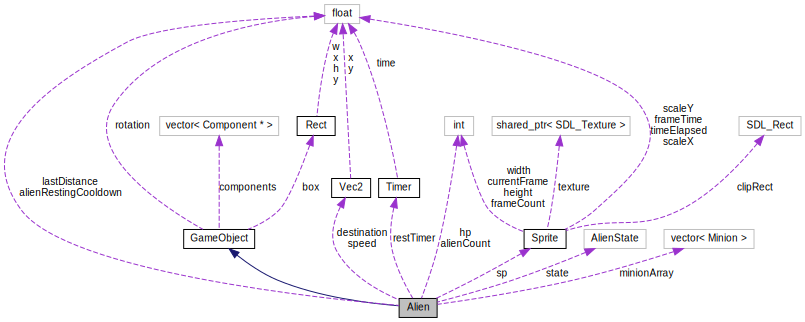
\includegraphics[width=350pt]{classAlien__coll__graph}
\end{center}
\end{figure}
\subsection*{Métodos Públicos}
\begin{DoxyCompactItemize}
\item 
\hyperlink{classAlien_ac5669bcecd6fb077cb7e6450a72105f4}{Alien} (float X, float y, int n\+Minions)
\item 
\hyperlink{classAlien_a2db6b66f06d32b6c8c689255e35e2f92}{$\sim$\+Alien} (void)
\item 
void \hyperlink{classAlien_a5bcca286b1a9d8f3fc56a2e8d5636b19}{Update} (float dt)
\item 
void \hyperlink{classAlien_a43e7b457eb4f8c41deae1a37aaf8622c}{Render} (void)
\item 
bool \hyperlink{classAlien_a27d2042c7097c2d37bb0268575ec8bad}{Is\+Dead} (void)
\item 
void \hyperlink{classAlien_a47baef9f1b44ad393b268812b752bd3a}{Notify\+Collision} (\hyperlink{classGameObject}{Game\+Object} \&other)
\item 
bool \hyperlink{classAlien_a9697e1dc132cc829d787c8bd586a01a2}{Is} (string type)
\end{DoxyCompactItemize}
\subsection*{Atributos Estáticos Públicos}
\begin{DoxyCompactItemize}
\item 
static int \hyperlink{classAlien_abde06bf01bdb2d9786b7815d0db5d17d}{alien\+Count} =0
\end{DoxyCompactItemize}
\subsection*{Tipos Privados}
\begin{DoxyCompactItemize}
\item 
enum \hyperlink{classAlien_ae23fef43ed399f4b117ccf0520173455}{Alien\+State} \{ \hyperlink{classAlien_ae23fef43ed399f4b117ccf0520173455afbdbebbbfd9cfe581a6934b67727c99b}{M\+O\+V\+I\+N\+G}, 
\hyperlink{classAlien_ae23fef43ed399f4b117ccf0520173455a2a5c16b3119d8a7466ca285159173710}{R\+E\+S\+T\+I\+N\+G}
 \}
\end{DoxyCompactItemize}
\subsection*{Métodos Privados}
\begin{DoxyCompactItemize}
\item 
int \hyperlink{classAlien_a1364c1ebddf1cebfdcee250a2b1f82f9}{Get\+Nearest\+Minion} (\hyperlink{classVec2}{Vec2} target\+Pos)
\item 
float \hyperlink{classAlien_a39926c487410c1604b7d4f330ead6adf}{Calculate\+Resting\+Cooldown} (void)
\end{DoxyCompactItemize}
\subsection*{Atributos Privados}
\begin{DoxyCompactItemize}
\item 
enum \hyperlink{classAlien_ae23fef43ed399f4b117ccf0520173455}{Alien\+::\+Alien\+State} \hyperlink{classAlien_a595501207125bf8bb67a2b07c6e580dd}{state}
\item 
\hyperlink{classSprite}{Sprite} \hyperlink{classAlien_a353c0cf8e9bb3b689b34866b3c3ac0f7}{sp}
\item 
\hyperlink{classVec2}{Vec2} \hyperlink{classAlien_a3acafe16e399a54c4d2511aad4f96cd4}{speed}
\item 
int \hyperlink{classAlien_ad88d130f8e4538ecbeede37e05f2bf32}{hp}
\item 
vector$<$ \hyperlink{classMinion}{Minion} $>$ \hyperlink{classAlien_a2ce0b76dc42b78ef26f1c524e428f682}{minion\+Array}
\item 
\hyperlink{classTimer}{Timer} \hyperlink{classAlien_a1045a69ebda8020e122db9021398098a}{rest\+Timer}
\item 
\hyperlink{classVec2}{Vec2} \hyperlink{classAlien_a9534c5cc95f08a23c91ffd8ea7fbc116}{destination}
\item 
float \hyperlink{classAlien_a61538503ff1bde408267d85464191fe4}{alien\+Resting\+Cooldown}
\item 
float \hyperlink{classAlien_a0f671a6a6f32d951a2406c87d9f18963}{last\+Distance}
\end{DoxyCompactItemize}
\subsection*{Additional Inherited Members}


\subsection{Enumerações}
\hypertarget{classAlien_ae23fef43ed399f4b117ccf0520173455}{\index{Alien@{Alien}!Alien\+State@{Alien\+State}}
\index{Alien\+State@{Alien\+State}!Alien@{Alien}}
\subsubsection[{Alien\+State}]{\setlength{\rightskip}{0pt plus 5cm}enum {\bf Alien\+::\+Alien\+State}\hspace{0.3cm}{\ttfamily [private]}}}\label{classAlien_ae23fef43ed399f4b117ccf0520173455}
\begin{Desc}
\item[Valores enumerados]\par
\begin{description}
\index{M\+O\+V\+I\+N\+G@{M\+O\+V\+I\+N\+G}!Alien@{Alien}}\index{Alien@{Alien}!M\+O\+V\+I\+N\+G@{M\+O\+V\+I\+N\+G}}\item[{\em 
\hypertarget{classAlien_ae23fef43ed399f4b117ccf0520173455afbdbebbbfd9cfe581a6934b67727c99b}{M\+O\+V\+I\+N\+G}\label{classAlien_ae23fef43ed399f4b117ccf0520173455afbdbebbbfd9cfe581a6934b67727c99b}
}]\index{R\+E\+S\+T\+I\+N\+G@{R\+E\+S\+T\+I\+N\+G}!Alien@{Alien}}\index{Alien@{Alien}!R\+E\+S\+T\+I\+N\+G@{R\+E\+S\+T\+I\+N\+G}}\item[{\em 
\hypertarget{classAlien_ae23fef43ed399f4b117ccf0520173455a2a5c16b3119d8a7466ca285159173710}{R\+E\+S\+T\+I\+N\+G}\label{classAlien_ae23fef43ed399f4b117ccf0520173455a2a5c16b3119d8a7466ca285159173710}
}]\end{description}
\end{Desc}


\subsection{Construtores \& Destrutores}
\hypertarget{classAlien_ac5669bcecd6fb077cb7e6450a72105f4}{\index{Alien@{Alien}!Alien@{Alien}}
\index{Alien@{Alien}!Alien@{Alien}}
\subsubsection[{Alien}]{\setlength{\rightskip}{0pt plus 5cm}Alien\+::\+Alien (
\begin{DoxyParamCaption}
\item[{float}]{X, }
\item[{float}]{y, }
\item[{int}]{n\+Minions}
\end{DoxyParamCaption}
)}}\label{classAlien_ac5669bcecd6fb077cb7e6450a72105f4}
\hypertarget{classAlien_a2db6b66f06d32b6c8c689255e35e2f92}{\index{Alien@{Alien}!````~Alien@{$\sim$\+Alien}}
\index{````~Alien@{$\sim$\+Alien}!Alien@{Alien}}
\subsubsection[{$\sim$\+Alien}]{\setlength{\rightskip}{0pt plus 5cm}Alien\+::$\sim$\+Alien (
\begin{DoxyParamCaption}
\item[{void}]{}
\end{DoxyParamCaption}
)}}\label{classAlien_a2db6b66f06d32b6c8c689255e35e2f92}


\subsection{Métodos}
\hypertarget{classAlien_a39926c487410c1604b7d4f330ead6adf}{\index{Alien@{Alien}!Calculate\+Resting\+Cooldown@{Calculate\+Resting\+Cooldown}}
\index{Calculate\+Resting\+Cooldown@{Calculate\+Resting\+Cooldown}!Alien@{Alien}}
\subsubsection[{Calculate\+Resting\+Cooldown}]{\setlength{\rightskip}{0pt plus 5cm}float Alien\+::\+Calculate\+Resting\+Cooldown (
\begin{DoxyParamCaption}
\item[{void}]{}
\end{DoxyParamCaption}
)\hspace{0.3cm}{\ttfamily [private]}}}\label{classAlien_a39926c487410c1604b7d4f330ead6adf}
\hypertarget{classAlien_a1364c1ebddf1cebfdcee250a2b1f82f9}{\index{Alien@{Alien}!Get\+Nearest\+Minion@{Get\+Nearest\+Minion}}
\index{Get\+Nearest\+Minion@{Get\+Nearest\+Minion}!Alien@{Alien}}
\subsubsection[{Get\+Nearest\+Minion}]{\setlength{\rightskip}{0pt plus 5cm}int Alien\+::\+Get\+Nearest\+Minion (
\begin{DoxyParamCaption}
\item[{{\bf Vec2}}]{target\+Pos}
\end{DoxyParamCaption}
)\hspace{0.3cm}{\ttfamily [private]}}}\label{classAlien_a1364c1ebddf1cebfdcee250a2b1f82f9}
\hypertarget{classAlien_a9697e1dc132cc829d787c8bd586a01a2}{\index{Alien@{Alien}!Is@{Is}}
\index{Is@{Is}!Alien@{Alien}}
\subsubsection[{Is}]{\setlength{\rightskip}{0pt plus 5cm}bool Alien\+::\+Is (
\begin{DoxyParamCaption}
\item[{string}]{type}
\end{DoxyParamCaption}
)\hspace{0.3cm}{\ttfamily [virtual]}}}\label{classAlien_a9697e1dc132cc829d787c8bd586a01a2}


Implementa \hyperlink{classGameObject_a3ddba599a800d774463c7082b7ef4801}{Game\+Object}.

\hypertarget{classAlien_a27d2042c7097c2d37bb0268575ec8bad}{\index{Alien@{Alien}!Is\+Dead@{Is\+Dead}}
\index{Is\+Dead@{Is\+Dead}!Alien@{Alien}}
\subsubsection[{Is\+Dead}]{\setlength{\rightskip}{0pt plus 5cm}bool Alien\+::\+Is\+Dead (
\begin{DoxyParamCaption}
\item[{void}]{}
\end{DoxyParamCaption}
)\hspace{0.3cm}{\ttfamily [virtual]}}}\label{classAlien_a27d2042c7097c2d37bb0268575ec8bad}


Implementa \hyperlink{classGameObject_a076afa2ea9190c49046f86a0946b4543}{Game\+Object}.

\hypertarget{classAlien_a47baef9f1b44ad393b268812b752bd3a}{\index{Alien@{Alien}!Notify\+Collision@{Notify\+Collision}}
\index{Notify\+Collision@{Notify\+Collision}!Alien@{Alien}}
\subsubsection[{Notify\+Collision}]{\setlength{\rightskip}{0pt plus 5cm}void Alien\+::\+Notify\+Collision (
\begin{DoxyParamCaption}
\item[{{\bf Game\+Object} \&}]{other}
\end{DoxyParamCaption}
)\hspace{0.3cm}{\ttfamily [virtual]}}}\label{classAlien_a47baef9f1b44ad393b268812b752bd3a}


Implementa \hyperlink{classGameObject_aa627e6c2913983fc5f108c1c4d303eb8}{Game\+Object}.

\hypertarget{classAlien_a43e7b457eb4f8c41deae1a37aaf8622c}{\index{Alien@{Alien}!Render@{Render}}
\index{Render@{Render}!Alien@{Alien}}
\subsubsection[{Render}]{\setlength{\rightskip}{0pt plus 5cm}void Alien\+::\+Render (
\begin{DoxyParamCaption}
\item[{void}]{}
\end{DoxyParamCaption}
)\hspace{0.3cm}{\ttfamily [virtual]}}}\label{classAlien_a43e7b457eb4f8c41deae1a37aaf8622c}


Implementa \hyperlink{classGameObject_a976b9c0d72212389603802f95b3f3424}{Game\+Object}.

\hypertarget{classAlien_a5bcca286b1a9d8f3fc56a2e8d5636b19}{\index{Alien@{Alien}!Update@{Update}}
\index{Update@{Update}!Alien@{Alien}}
\subsubsection[{Update}]{\setlength{\rightskip}{0pt plus 5cm}void Alien\+::\+Update (
\begin{DoxyParamCaption}
\item[{float}]{dt}
\end{DoxyParamCaption}
)\hspace{0.3cm}{\ttfamily [virtual]}}}\label{classAlien_a5bcca286b1a9d8f3fc56a2e8d5636b19}


Implementa \hyperlink{classGameObject_a93ed63df640deb516a020530e7f8e045}{Game\+Object}.



\subsection{Atributos}
\hypertarget{classAlien_abde06bf01bdb2d9786b7815d0db5d17d}{\index{Alien@{Alien}!alien\+Count@{alien\+Count}}
\index{alien\+Count@{alien\+Count}!Alien@{Alien}}
\subsubsection[{alien\+Count}]{\setlength{\rightskip}{0pt plus 5cm}int Alien\+::alien\+Count =0\hspace{0.3cm}{\ttfamily [static]}}}\label{classAlien_abde06bf01bdb2d9786b7815d0db5d17d}
\hypertarget{classAlien_a61538503ff1bde408267d85464191fe4}{\index{Alien@{Alien}!alien\+Resting\+Cooldown@{alien\+Resting\+Cooldown}}
\index{alien\+Resting\+Cooldown@{alien\+Resting\+Cooldown}!Alien@{Alien}}
\subsubsection[{alien\+Resting\+Cooldown}]{\setlength{\rightskip}{0pt plus 5cm}float Alien\+::alien\+Resting\+Cooldown\hspace{0.3cm}{\ttfamily [private]}}}\label{classAlien_a61538503ff1bde408267d85464191fe4}
\hypertarget{classAlien_a9534c5cc95f08a23c91ffd8ea7fbc116}{\index{Alien@{Alien}!destination@{destination}}
\index{destination@{destination}!Alien@{Alien}}
\subsubsection[{destination}]{\setlength{\rightskip}{0pt plus 5cm}{\bf Vec2} Alien\+::destination\hspace{0.3cm}{\ttfamily [private]}}}\label{classAlien_a9534c5cc95f08a23c91ffd8ea7fbc116}
\hypertarget{classAlien_ad88d130f8e4538ecbeede37e05f2bf32}{\index{Alien@{Alien}!hp@{hp}}
\index{hp@{hp}!Alien@{Alien}}
\subsubsection[{hp}]{\setlength{\rightskip}{0pt plus 5cm}int Alien\+::hp\hspace{0.3cm}{\ttfamily [private]}}}\label{classAlien_ad88d130f8e4538ecbeede37e05f2bf32}
\hypertarget{classAlien_a0f671a6a6f32d951a2406c87d9f18963}{\index{Alien@{Alien}!last\+Distance@{last\+Distance}}
\index{last\+Distance@{last\+Distance}!Alien@{Alien}}
\subsubsection[{last\+Distance}]{\setlength{\rightskip}{0pt plus 5cm}float Alien\+::last\+Distance\hspace{0.3cm}{\ttfamily [private]}}}\label{classAlien_a0f671a6a6f32d951a2406c87d9f18963}
\hypertarget{classAlien_a2ce0b76dc42b78ef26f1c524e428f682}{\index{Alien@{Alien}!minion\+Array@{minion\+Array}}
\index{minion\+Array@{minion\+Array}!Alien@{Alien}}
\subsubsection[{minion\+Array}]{\setlength{\rightskip}{0pt plus 5cm}vector$<${\bf Minion}$>$ Alien\+::minion\+Array\hspace{0.3cm}{\ttfamily [private]}}}\label{classAlien_a2ce0b76dc42b78ef26f1c524e428f682}
\hypertarget{classAlien_a1045a69ebda8020e122db9021398098a}{\index{Alien@{Alien}!rest\+Timer@{rest\+Timer}}
\index{rest\+Timer@{rest\+Timer}!Alien@{Alien}}
\subsubsection[{rest\+Timer}]{\setlength{\rightskip}{0pt plus 5cm}{\bf Timer} Alien\+::rest\+Timer\hspace{0.3cm}{\ttfamily [private]}}}\label{classAlien_a1045a69ebda8020e122db9021398098a}
\hypertarget{classAlien_a353c0cf8e9bb3b689b34866b3c3ac0f7}{\index{Alien@{Alien}!sp@{sp}}
\index{sp@{sp}!Alien@{Alien}}
\subsubsection[{sp}]{\setlength{\rightskip}{0pt plus 5cm}{\bf Sprite} Alien\+::sp\hspace{0.3cm}{\ttfamily [private]}}}\label{classAlien_a353c0cf8e9bb3b689b34866b3c3ac0f7}
\hypertarget{classAlien_a3acafe16e399a54c4d2511aad4f96cd4}{\index{Alien@{Alien}!speed@{speed}}
\index{speed@{speed}!Alien@{Alien}}
\subsubsection[{speed}]{\setlength{\rightskip}{0pt plus 5cm}{\bf Vec2} Alien\+::speed\hspace{0.3cm}{\ttfamily [private]}}}\label{classAlien_a3acafe16e399a54c4d2511aad4f96cd4}
\hypertarget{classAlien_a595501207125bf8bb67a2b07c6e580dd}{\index{Alien@{Alien}!state@{state}}
\index{state@{state}!Alien@{Alien}}
\subsubsection[{state}]{\setlength{\rightskip}{0pt plus 5cm}enum {\bf Alien\+::\+Alien\+State}  Alien\+::state\hspace{0.3cm}{\ttfamily [private]}}}\label{classAlien_a595501207125bf8bb67a2b07c6e580dd}


A documentação para esta classe foi gerada a partir dos seguintes arquivos\+:\begin{DoxyCompactItemize}
\item 
Game/include/\hyperlink{Alien_8h}{Alien.\+h}\item 
Game/src/\hyperlink{Alien_8cpp}{Alien.\+cpp}\end{DoxyCompactItemize}

\hypertarget{classAnimation}{\section{Referência da Classe Animation}
\label{classAnimation}\index{Animation@{Animation}}
}


{\ttfamily \#include $<$Animation.\+h$>$}



Diagrama de Hierarquia para Animation\+:\nopagebreak
\begin{figure}[H]
\begin{center}
\leavevmode
\includegraphics[width=151pt]{classAnimation__inherit__graph}
\end{center}
\end{figure}


Diagrama de colaboração para Animation\+:
\nopagebreak
\begin{figure}[H]
\begin{center}
\leavevmode
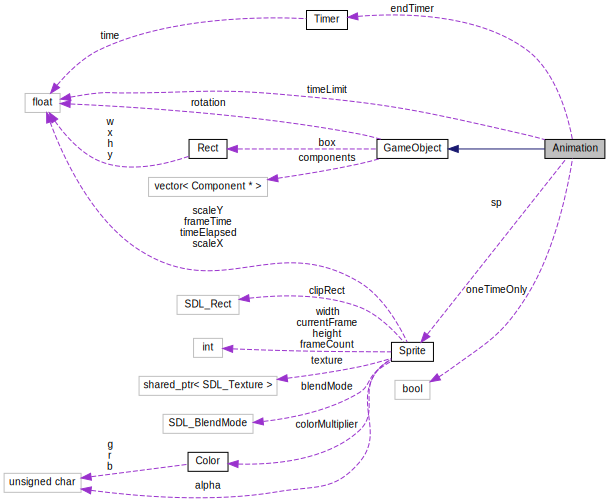
\includegraphics[width=350pt]{classAnimation__coll__graph}
\end{center}
\end{figure}
\subsection*{Métodos Públicos}
\begin{DoxyCompactItemize}
\item 
\hyperlink{classAnimation_a48d3ca5ecd4b4ca7f2f6fe10cf1f91d4}{Animation} (float x, float y, float \hyperlink{classGameObject_ac55f6ebdf4cfbab508680ad7290fb26c}{rotation}, string sprite, int frame\+Count, float frame\+Time, bool ends)
\item 
void \hyperlink{classAnimation_a1871db60d1fb351aeb77ada38dd4dd9c}{Update} (float dt)
\item 
void \hyperlink{classAnimation_a49749e3890cec3896e6f726323544c26}{Render} (void)
\item 
bool \hyperlink{classAnimation_ad1eaa9ff240cbcc114270ea174523702}{Is\+Dead} (void)
\item 
void \hyperlink{classAnimation_a611b21418311eb697ec4af1aaff92657}{Notify\+Collision} (\hyperlink{classGameObject}{Game\+Object} \&other)
\item 
bool \hyperlink{classAnimation_a166f36012f3092275648a74272e8ff0f}{Is} (string type)
\end{DoxyCompactItemize}
\subsection*{Atributos Privados}
\begin{DoxyCompactItemize}
\item 
\hyperlink{classTimer}{Timer} \hyperlink{classAnimation_ad4e2674025e4f91143e574c09e213e38}{end\+Timer}
\item 
float \hyperlink{classAnimation_ab8b4a075f8bf097b7af6e732949235c6}{time\+Limit}
\item 
bool \hyperlink{classAnimation_aa8be050af14ac86c2cce45908bae750d}{onetime\+Only}
\item 
\hyperlink{classSprite}{Sprite} \hyperlink{classAnimation_abf968c115c1d8c88da797215d58ad516}{sp}
\end{DoxyCompactItemize}
\subsection*{Additional Inherited Members}


\subsection{Construtores \& Destrutores}
\hypertarget{classAnimation_a48d3ca5ecd4b4ca7f2f6fe10cf1f91d4}{\index{Animation@{Animation}!Animation@{Animation}}
\index{Animation@{Animation}!Animation@{Animation}}
\subsubsection[{Animation}]{\setlength{\rightskip}{0pt plus 5cm}Animation\+::\+Animation (
\begin{DoxyParamCaption}
\item[{float}]{x, }
\item[{float}]{y, }
\item[{float}]{rotation, }
\item[{string}]{sprite, }
\item[{int}]{frame\+Count, }
\item[{float}]{frame\+Time, }
\item[{bool}]{ends}
\end{DoxyParamCaption}
)}}\label{classAnimation_a48d3ca5ecd4b4ca7f2f6fe10cf1f91d4}


\subsection{Métodos}
\hypertarget{classAnimation_a166f36012f3092275648a74272e8ff0f}{\index{Animation@{Animation}!Is@{Is}}
\index{Is@{Is}!Animation@{Animation}}
\subsubsection[{Is}]{\setlength{\rightskip}{0pt plus 5cm}bool Animation\+::\+Is (
\begin{DoxyParamCaption}
\item[{string}]{type}
\end{DoxyParamCaption}
)\hspace{0.3cm}{\ttfamily [virtual]}}}\label{classAnimation_a166f36012f3092275648a74272e8ff0f}


Implementa \hyperlink{classGameObject_a3ddba599a800d774463c7082b7ef4801}{Game\+Object}.

\hypertarget{classAnimation_ad1eaa9ff240cbcc114270ea174523702}{\index{Animation@{Animation}!Is\+Dead@{Is\+Dead}}
\index{Is\+Dead@{Is\+Dead}!Animation@{Animation}}
\subsubsection[{Is\+Dead}]{\setlength{\rightskip}{0pt plus 5cm}bool Animation\+::\+Is\+Dead (
\begin{DoxyParamCaption}
\item[{void}]{}
\end{DoxyParamCaption}
)\hspace{0.3cm}{\ttfamily [virtual]}}}\label{classAnimation_ad1eaa9ff240cbcc114270ea174523702}


Implementa \hyperlink{classGameObject_a076afa2ea9190c49046f86a0946b4543}{Game\+Object}.

\hypertarget{classAnimation_a611b21418311eb697ec4af1aaff92657}{\index{Animation@{Animation}!Notify\+Collision@{Notify\+Collision}}
\index{Notify\+Collision@{Notify\+Collision}!Animation@{Animation}}
\subsubsection[{Notify\+Collision}]{\setlength{\rightskip}{0pt plus 5cm}void Animation\+::\+Notify\+Collision (
\begin{DoxyParamCaption}
\item[{{\bf Game\+Object} \&}]{other}
\end{DoxyParamCaption}
)\hspace{0.3cm}{\ttfamily [virtual]}}}\label{classAnimation_a611b21418311eb697ec4af1aaff92657}


Implementa \hyperlink{classGameObject_aa627e6c2913983fc5f108c1c4d303eb8}{Game\+Object}.

\hypertarget{classAnimation_a49749e3890cec3896e6f726323544c26}{\index{Animation@{Animation}!Render@{Render}}
\index{Render@{Render}!Animation@{Animation}}
\subsubsection[{Render}]{\setlength{\rightskip}{0pt plus 5cm}void Animation\+::\+Render (
\begin{DoxyParamCaption}
\item[{void}]{}
\end{DoxyParamCaption}
)\hspace{0.3cm}{\ttfamily [virtual]}}}\label{classAnimation_a49749e3890cec3896e6f726323544c26}


Implementa \hyperlink{classGameObject_a976b9c0d72212389603802f95b3f3424}{Game\+Object}.

\hypertarget{classAnimation_a1871db60d1fb351aeb77ada38dd4dd9c}{\index{Animation@{Animation}!Update@{Update}}
\index{Update@{Update}!Animation@{Animation}}
\subsubsection[{Update}]{\setlength{\rightskip}{0pt plus 5cm}void Animation\+::\+Update (
\begin{DoxyParamCaption}
\item[{float}]{dt}
\end{DoxyParamCaption}
)\hspace{0.3cm}{\ttfamily [virtual]}}}\label{classAnimation_a1871db60d1fb351aeb77ada38dd4dd9c}


Implementa \hyperlink{classGameObject_a93ed63df640deb516a020530e7f8e045}{Game\+Object}.



\subsection{Atributos}
\hypertarget{classAnimation_ad4e2674025e4f91143e574c09e213e38}{\index{Animation@{Animation}!end\+Timer@{end\+Timer}}
\index{end\+Timer@{end\+Timer}!Animation@{Animation}}
\subsubsection[{end\+Timer}]{\setlength{\rightskip}{0pt plus 5cm}{\bf Timer} Animation\+::end\+Timer\hspace{0.3cm}{\ttfamily [private]}}}\label{classAnimation_ad4e2674025e4f91143e574c09e213e38}
\hypertarget{classAnimation_aa8be050af14ac86c2cce45908bae750d}{\index{Animation@{Animation}!onetime\+Only@{onetime\+Only}}
\index{onetime\+Only@{onetime\+Only}!Animation@{Animation}}
\subsubsection[{onetime\+Only}]{\setlength{\rightskip}{0pt plus 5cm}bool Animation\+::onetime\+Only\hspace{0.3cm}{\ttfamily [private]}}}\label{classAnimation_aa8be050af14ac86c2cce45908bae750d}
\hypertarget{classAnimation_abf968c115c1d8c88da797215d58ad516}{\index{Animation@{Animation}!sp@{sp}}
\index{sp@{sp}!Animation@{Animation}}
\subsubsection[{sp}]{\setlength{\rightskip}{0pt plus 5cm}{\bf Sprite} Animation\+::sp\hspace{0.3cm}{\ttfamily [private]}}}\label{classAnimation_abf968c115c1d8c88da797215d58ad516}
\hypertarget{classAnimation_ab8b4a075f8bf097b7af6e732949235c6}{\index{Animation@{Animation}!time\+Limit@{time\+Limit}}
\index{time\+Limit@{time\+Limit}!Animation@{Animation}}
\subsubsection[{time\+Limit}]{\setlength{\rightskip}{0pt plus 5cm}float Animation\+::time\+Limit\hspace{0.3cm}{\ttfamily [private]}}}\label{classAnimation_ab8b4a075f8bf097b7af6e732949235c6}


A documentação para esta classe foi gerada a partir dos seguintes arquivos\+:\begin{DoxyCompactItemize}
\item 
Engine/include/\hyperlink{Animation_8h}{Animation.\+h}\item 
Engine/src/\hyperlink{Animation_8cpp}{Animation.\+cpp}\end{DoxyCompactItemize}

\hypertarget{classBullet}{\section{Referência da Classe Bullet}
\label{classBullet}\index{Bullet@{Bullet}}
}


{\ttfamily \#include $<$Bullet.\+h$>$}



Diagrama de Hierarquia para Bullet\+:\nopagebreak
\begin{figure}[H]
\begin{center}
\leavevmode
\includegraphics[width=151pt]{classBullet__inherit__graph}
\end{center}
\end{figure}


Diagrama de colaboração para Bullet\+:
\nopagebreak
\begin{figure}[H]
\begin{center}
\leavevmode
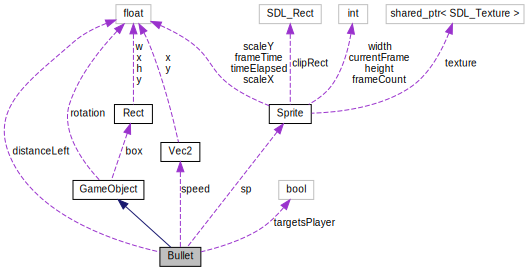
\includegraphics[width=350pt]{classBullet__coll__graph}
\end{center}
\end{figure}
\subsection*{Métodos Públicos}
\begin{DoxyCompactItemize}
\item 
\hyperlink{classBullet_a509f1d8e6f7629934574c15c835de0c8}{Bullet} (float x, float y, float angle, float \hyperlink{classBullet_a9674d36173dafc258455bbaa9b39b326}{speed}, float max\+Distance, float frame\+Time, int frame\+Count, string sprite, bool \hyperlink{classBullet_a57270bc61a381861bd548a7f2466bca2}{targets\+Player})
\item 
\hyperlink{classBullet_ab3c2b9c0b12c18aeace52bd289ddfce3}{$\sim$\+Bullet} (void)
\item 
void \hyperlink{classBullet_a5ca74d7990f25c518df1860b681079ea}{Update} (float dt)
\item 
void \hyperlink{classBullet_aace1e49986271afb6384d15bf40a0e92}{Render} (void)
\item 
bool \hyperlink{classBullet_a17cf15fdfa0c42931f21828feed2a77d}{Is\+Dead} (void)
\item 
void \hyperlink{classBullet_a272c1b019f46df9ad9bd45bd9ffb6e41}{Notify\+Collision} (\hyperlink{classGameObject}{Game\+Object} \&other)
\item 
bool \hyperlink{classBullet_aaa159cc9dcc3e7c780bbccc1ebc6d95a}{Is} (string type)
\item 
bool \hyperlink{classBullet_a293a665825d9e32c798d8fe669fcf695}{Targets\+Player} (void) const 
\end{DoxyCompactItemize}
\subsection*{Atributos Privados}
\begin{DoxyCompactItemize}
\item 
\hyperlink{classSprite}{Sprite} \hyperlink{classBullet_a3b796813022508f0f5f821c2a90ac863}{sp}
\item 
\hyperlink{classVec2}{Vec2} \hyperlink{classBullet_a9674d36173dafc258455bbaa9b39b326}{speed}
\item 
float \hyperlink{classBullet_ac24a38eea713d69e34c090416177b426}{distance\+Left}
\item 
bool \hyperlink{classBullet_a57270bc61a381861bd548a7f2466bca2}{targets\+Player}
\end{DoxyCompactItemize}
\subsection*{Additional Inherited Members}


\subsection{Construtores \& Destrutores}
\hypertarget{classBullet_a509f1d8e6f7629934574c15c835de0c8}{\index{Bullet@{Bullet}!Bullet@{Bullet}}
\index{Bullet@{Bullet}!Bullet@{Bullet}}
\subsubsection[{Bullet}]{\setlength{\rightskip}{0pt plus 5cm}Bullet\+::\+Bullet (
\begin{DoxyParamCaption}
\item[{float}]{x, }
\item[{float}]{y, }
\item[{float}]{angle, }
\item[{float}]{speed, }
\item[{float}]{max\+Distance, }
\item[{float}]{frame\+Time, }
\item[{int}]{frame\+Count, }
\item[{string}]{sprite, }
\item[{bool}]{targets\+Player}
\end{DoxyParamCaption}
)}}\label{classBullet_a509f1d8e6f7629934574c15c835de0c8}
\hypertarget{classBullet_ab3c2b9c0b12c18aeace52bd289ddfce3}{\index{Bullet@{Bullet}!````~Bullet@{$\sim$\+Bullet}}
\index{````~Bullet@{$\sim$\+Bullet}!Bullet@{Bullet}}
\subsubsection[{$\sim$\+Bullet}]{\setlength{\rightskip}{0pt plus 5cm}Bullet\+::$\sim$\+Bullet (
\begin{DoxyParamCaption}
\item[{void}]{}
\end{DoxyParamCaption}
)}}\label{classBullet_ab3c2b9c0b12c18aeace52bd289ddfce3}


\subsection{Métodos}
\hypertarget{classBullet_aaa159cc9dcc3e7c780bbccc1ebc6d95a}{\index{Bullet@{Bullet}!Is@{Is}}
\index{Is@{Is}!Bullet@{Bullet}}
\subsubsection[{Is}]{\setlength{\rightskip}{0pt plus 5cm}bool Bullet\+::\+Is (
\begin{DoxyParamCaption}
\item[{string}]{type}
\end{DoxyParamCaption}
)\hspace{0.3cm}{\ttfamily [virtual]}}}\label{classBullet_aaa159cc9dcc3e7c780bbccc1ebc6d95a}


Implementa \hyperlink{classGameObject_a3ddba599a800d774463c7082b7ef4801}{Game\+Object}.

\hypertarget{classBullet_a17cf15fdfa0c42931f21828feed2a77d}{\index{Bullet@{Bullet}!Is\+Dead@{Is\+Dead}}
\index{Is\+Dead@{Is\+Dead}!Bullet@{Bullet}}
\subsubsection[{Is\+Dead}]{\setlength{\rightskip}{0pt plus 5cm}bool Bullet\+::\+Is\+Dead (
\begin{DoxyParamCaption}
\item[{void}]{}
\end{DoxyParamCaption}
)\hspace{0.3cm}{\ttfamily [virtual]}}}\label{classBullet_a17cf15fdfa0c42931f21828feed2a77d}


Implementa \hyperlink{classGameObject_a076afa2ea9190c49046f86a0946b4543}{Game\+Object}.

\hypertarget{classBullet_a272c1b019f46df9ad9bd45bd9ffb6e41}{\index{Bullet@{Bullet}!Notify\+Collision@{Notify\+Collision}}
\index{Notify\+Collision@{Notify\+Collision}!Bullet@{Bullet}}
\subsubsection[{Notify\+Collision}]{\setlength{\rightskip}{0pt plus 5cm}void Bullet\+::\+Notify\+Collision (
\begin{DoxyParamCaption}
\item[{{\bf Game\+Object} \&}]{other}
\end{DoxyParamCaption}
)\hspace{0.3cm}{\ttfamily [virtual]}}}\label{classBullet_a272c1b019f46df9ad9bd45bd9ffb6e41}


Implementa \hyperlink{classGameObject_aa627e6c2913983fc5f108c1c4d303eb8}{Game\+Object}.

\hypertarget{classBullet_aace1e49986271afb6384d15bf40a0e92}{\index{Bullet@{Bullet}!Render@{Render}}
\index{Render@{Render}!Bullet@{Bullet}}
\subsubsection[{Render}]{\setlength{\rightskip}{0pt plus 5cm}void Bullet\+::\+Render (
\begin{DoxyParamCaption}
\item[{void}]{}
\end{DoxyParamCaption}
)\hspace{0.3cm}{\ttfamily [virtual]}}}\label{classBullet_aace1e49986271afb6384d15bf40a0e92}


Implementa \hyperlink{classGameObject_a976b9c0d72212389603802f95b3f3424}{Game\+Object}.

\hypertarget{classBullet_a293a665825d9e32c798d8fe669fcf695}{\index{Bullet@{Bullet}!Targets\+Player@{Targets\+Player}}
\index{Targets\+Player@{Targets\+Player}!Bullet@{Bullet}}
\subsubsection[{Targets\+Player}]{\setlength{\rightskip}{0pt plus 5cm}bool Bullet\+::\+Targets\+Player (
\begin{DoxyParamCaption}
\item[{void}]{}
\end{DoxyParamCaption}
) const}}\label{classBullet_a293a665825d9e32c798d8fe669fcf695}
\hypertarget{classBullet_a5ca74d7990f25c518df1860b681079ea}{\index{Bullet@{Bullet}!Update@{Update}}
\index{Update@{Update}!Bullet@{Bullet}}
\subsubsection[{Update}]{\setlength{\rightskip}{0pt plus 5cm}void Bullet\+::\+Update (
\begin{DoxyParamCaption}
\item[{float}]{dt}
\end{DoxyParamCaption}
)\hspace{0.3cm}{\ttfamily [virtual]}}}\label{classBullet_a5ca74d7990f25c518df1860b681079ea}


Implementa \hyperlink{classGameObject_a93ed63df640deb516a020530e7f8e045}{Game\+Object}.



\subsection{Atributos}
\hypertarget{classBullet_ac24a38eea713d69e34c090416177b426}{\index{Bullet@{Bullet}!distance\+Left@{distance\+Left}}
\index{distance\+Left@{distance\+Left}!Bullet@{Bullet}}
\subsubsection[{distance\+Left}]{\setlength{\rightskip}{0pt plus 5cm}float Bullet\+::distance\+Left\hspace{0.3cm}{\ttfamily [private]}}}\label{classBullet_ac24a38eea713d69e34c090416177b426}
\hypertarget{classBullet_a3b796813022508f0f5f821c2a90ac863}{\index{Bullet@{Bullet}!sp@{sp}}
\index{sp@{sp}!Bullet@{Bullet}}
\subsubsection[{sp}]{\setlength{\rightskip}{0pt plus 5cm}{\bf Sprite} Bullet\+::sp\hspace{0.3cm}{\ttfamily [private]}}}\label{classBullet_a3b796813022508f0f5f821c2a90ac863}
\hypertarget{classBullet_a9674d36173dafc258455bbaa9b39b326}{\index{Bullet@{Bullet}!speed@{speed}}
\index{speed@{speed}!Bullet@{Bullet}}
\subsubsection[{speed}]{\setlength{\rightskip}{0pt plus 5cm}{\bf Vec2} Bullet\+::speed\hspace{0.3cm}{\ttfamily [private]}}}\label{classBullet_a9674d36173dafc258455bbaa9b39b326}
\hypertarget{classBullet_a57270bc61a381861bd548a7f2466bca2}{\index{Bullet@{Bullet}!targets\+Player@{targets\+Player}}
\index{targets\+Player@{targets\+Player}!Bullet@{Bullet}}
\subsubsection[{targets\+Player}]{\setlength{\rightskip}{0pt plus 5cm}bool Bullet\+::targets\+Player\hspace{0.3cm}{\ttfamily [private]}}}\label{classBullet_a57270bc61a381861bd548a7f2466bca2}


A documentação para esta classe foi gerada a partir dos seguintes arquivos\+:\begin{DoxyCompactItemize}
\item 
Game/include/\hyperlink{Bullet_8h}{Bullet.\+h}\item 
Game/src/\hyperlink{Bullet_8cpp}{Bullet.\+cpp}\end{DoxyCompactItemize}

\hypertarget{classCamera}{\section{Referência da Classe Camera}
\label{classCamera}\index{Camera@{Camera}}
}


{\ttfamily \#include $<$Camera.\+h$>$}



Diagrama de colaboração para Camera\+:
\nopagebreak
\begin{figure}[H]
\begin{center}
\leavevmode
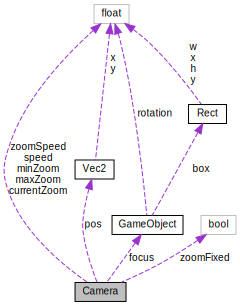
\includegraphics[width=317pt]{classCamera__coll__graph}
\end{center}
\end{figure}
\subsection*{Métodos Públicos Estáticos}
\begin{DoxyCompactItemize}
\item 
static void \hyperlink{classCamera_a4290d7e4815d2e0726d88b743d44e8df}{Follow} (\hyperlink{classGameObject}{Game\+Object} $\ast$new\+Focus)
\item 
static void \hyperlink{classCamera_aa9ca7decdebf7147c9d6dc747e7d59e9}{Unfollow} (void)
\item 
static void \hyperlink{classCamera_a3d528df411b986596b652b61120ff302}{Update} (float dt)
\item 
static void \hyperlink{classCamera_a7dc4b1fd7f5e03ffb25d306fe81ee4c0}{Force\+Zoom} (float new\+Zoom)
\item 
static void \hyperlink{classCamera_a2919142c206574be101efc1230eb3c8d}{Set\+Zoomnable} (bool zoomnable)
\item 
static void \hyperlink{classCamera_ad6638a961e2fefbe69d4d7d0a0591fb6}{Zoom} (float delta\+Zoom)
\item 
static void \hyperlink{classCamera_aa320e33bcbe395cdad9f63887ea15689}{Set\+Zoom\+Limits} (float \hyperlink{classCamera_a65d5a8e5533b568224d9fc488bfdcb28}{min\+Zoom}=0, float \hyperlink{classCamera_af418b7887d39c773d73cb179c497a8da}{max\+Zoom}=0)
\item 
static float \hyperlink{classCamera_af6fe062fcf5e1e31224d4dd9f6cafa51}{Get\+Zoom} (void)
\item 
static void \hyperlink{classCamera_a4373a9b1baa7b98e4fe5859e0645baed}{Set\+Zoom\+Speed} (float new\+Zoom\+Speed)
\end{DoxyCompactItemize}
\subsection*{Atributos Estáticos Públicos}
\begin{DoxyCompactItemize}
\item 
static \hyperlink{classVec2}{Vec2} \hyperlink{classCamera_a748c4e2867e34f45a431a1d2dcc6fee2}{pos}
\item 
static \hyperlink{classVec2}{Vec2} \hyperlink{classCamera_aa0d0a54eb56182723dbd0ce61e0b3e8d}{speed}
\end{DoxyCompactItemize}
\subsection*{Métodos Privados}
\begin{DoxyCompactItemize}
\item 
\hyperlink{classCamera_a01f94c3543f56ede7af49dc778f19331}{Camera} ()
\end{DoxyCompactItemize}
\subsection*{Atributos Privados Estáticos}
\begin{DoxyCompactItemize}
\item 
static \hyperlink{classGameObject}{Game\+Object} $\ast$ \hyperlink{classCamera_a266c767efbe18088d7f79880f7e98998}{focus} = nullptr
\item 
static float \hyperlink{classCamera_ac867d6d379c0d052ae65d57c7c313970}{current\+Zoom} = 1.\+0
\item 
static float \hyperlink{classCamera_a65d5a8e5533b568224d9fc488bfdcb28}{min\+Zoom} = \hyperlink{Camera_8h_a00bdac33db330ffa8021dc36c85506fe}{C\+A\+M\+E\+R\+A\+\_\+\+D\+E\+F\+A\+U\+L\+T\+\_\+\+M\+I\+N\+\_\+\+Z\+O\+O\+M}
\item 
static float \hyperlink{classCamera_af418b7887d39c773d73cb179c497a8da}{max\+Zoom} = \hyperlink{Camera_8h_a53a75501f4f47ca972ec050b09df05a3}{C\+A\+M\+E\+R\+A\+\_\+\+D\+E\+F\+A\+U\+L\+T\+\_\+\+M\+A\+X\+\_\+\+Z\+O\+O\+M}
\item 
static bool \hyperlink{classCamera_a7f235a90f57567a0012ed8f4a52634ce}{zoom\+Fixed} = !\hyperlink{Camera_8h_a719f5e3a817ca056a76495044f676277}{C\+A\+M\+E\+R\+A\+\_\+\+D\+E\+F\+A\+U\+L\+T\+\_\+\+Z\+O\+O\+M\+A\+B\+L\+E}
\item 
static float \hyperlink{classCamera_a7ec8dd2dcb2c3446ba88ad30e2e195d9}{zoom\+Speed} = \hyperlink{Camera_8h_a896eaf751ce7e99c97bfaa76ca33f150}{C\+A\+M\+E\+R\+A\+\_\+\+D\+E\+F\+A\+U\+L\+T\+\_\+\+Z\+O\+O\+M\+\_\+\+S\+P\+E\+E\+D}
\end{DoxyCompactItemize}


\subsection{Construtores \& Destrutores}
\hypertarget{classCamera_a01f94c3543f56ede7af49dc778f19331}{\index{Camera@{Camera}!Camera@{Camera}}
\index{Camera@{Camera}!Camera@{Camera}}
\subsubsection[{Camera}]{\setlength{\rightskip}{0pt plus 5cm}Camera\+::\+Camera (
\begin{DoxyParamCaption}
{}
\end{DoxyParamCaption}
)\hspace{0.3cm}{\ttfamily [private]}}}\label{classCamera_a01f94c3543f56ede7af49dc778f19331}


\subsection{Métodos}
\hypertarget{classCamera_a4290d7e4815d2e0726d88b743d44e8df}{\index{Camera@{Camera}!Follow@{Follow}}
\index{Follow@{Follow}!Camera@{Camera}}
\subsubsection[{Follow}]{\setlength{\rightskip}{0pt plus 5cm}void Camera\+::\+Follow (
\begin{DoxyParamCaption}
\item[{{\bf Game\+Object} $\ast$}]{new\+Focus}
\end{DoxyParamCaption}
)\hspace{0.3cm}{\ttfamily [static]}}}\label{classCamera_a4290d7e4815d2e0726d88b743d44e8df}
\hypertarget{classCamera_a7dc4b1fd7f5e03ffb25d306fe81ee4c0}{\index{Camera@{Camera}!Force\+Zoom@{Force\+Zoom}}
\index{Force\+Zoom@{Force\+Zoom}!Camera@{Camera}}
\subsubsection[{Force\+Zoom}]{\setlength{\rightskip}{0pt plus 5cm}void Camera\+::\+Force\+Zoom (
\begin{DoxyParamCaption}
\item[{float}]{new\+Zoom}
\end{DoxyParamCaption}
)\hspace{0.3cm}{\ttfamily [static]}}}\label{classCamera_a7dc4b1fd7f5e03ffb25d306fe81ee4c0}
\hypertarget{classCamera_af6fe062fcf5e1e31224d4dd9f6cafa51}{\index{Camera@{Camera}!Get\+Zoom@{Get\+Zoom}}
\index{Get\+Zoom@{Get\+Zoom}!Camera@{Camera}}
\subsubsection[{Get\+Zoom}]{\setlength{\rightskip}{0pt plus 5cm}float Camera\+::\+Get\+Zoom (
\begin{DoxyParamCaption}
\item[{void}]{}
\end{DoxyParamCaption}
)\hspace{0.3cm}{\ttfamily [static]}}}\label{classCamera_af6fe062fcf5e1e31224d4dd9f6cafa51}
\hypertarget{classCamera_aa320e33bcbe395cdad9f63887ea15689}{\index{Camera@{Camera}!Set\+Zoom\+Limits@{Set\+Zoom\+Limits}}
\index{Set\+Zoom\+Limits@{Set\+Zoom\+Limits}!Camera@{Camera}}
\subsubsection[{Set\+Zoom\+Limits}]{\setlength{\rightskip}{0pt plus 5cm}void Camera\+::\+Set\+Zoom\+Limits (
\begin{DoxyParamCaption}
\item[{float}]{min\+Zoom = {\ttfamily 0}, }
\item[{float}]{max\+Zoom = {\ttfamily 0}}
\end{DoxyParamCaption}
)\hspace{0.3cm}{\ttfamily [static]}}}\label{classCamera_aa320e33bcbe395cdad9f63887ea15689}
\hypertarget{classCamera_a2919142c206574be101efc1230eb3c8d}{\index{Camera@{Camera}!Set\+Zoomnable@{Set\+Zoomnable}}
\index{Set\+Zoomnable@{Set\+Zoomnable}!Camera@{Camera}}
\subsubsection[{Set\+Zoomnable}]{\setlength{\rightskip}{0pt plus 5cm}void Camera\+::\+Set\+Zoomnable (
\begin{DoxyParamCaption}
\item[{bool}]{zoomnable}
\end{DoxyParamCaption}
)\hspace{0.3cm}{\ttfamily [static]}}}\label{classCamera_a2919142c206574be101efc1230eb3c8d}
\hypertarget{classCamera_a4373a9b1baa7b98e4fe5859e0645baed}{\index{Camera@{Camera}!Set\+Zoom\+Speed@{Set\+Zoom\+Speed}}
\index{Set\+Zoom\+Speed@{Set\+Zoom\+Speed}!Camera@{Camera}}
\subsubsection[{Set\+Zoom\+Speed}]{\setlength{\rightskip}{0pt plus 5cm}void Camera\+::\+Set\+Zoom\+Speed (
\begin{DoxyParamCaption}
\item[{float}]{new\+Zoom\+Speed}
\end{DoxyParamCaption}
)\hspace{0.3cm}{\ttfamily [static]}}}\label{classCamera_a4373a9b1baa7b98e4fe5859e0645baed}
\hypertarget{classCamera_aa9ca7decdebf7147c9d6dc747e7d59e9}{\index{Camera@{Camera}!Unfollow@{Unfollow}}
\index{Unfollow@{Unfollow}!Camera@{Camera}}
\subsubsection[{Unfollow}]{\setlength{\rightskip}{0pt plus 5cm}void Camera\+::\+Unfollow (
\begin{DoxyParamCaption}
\item[{void}]{}
\end{DoxyParamCaption}
)\hspace{0.3cm}{\ttfamily [static]}}}\label{classCamera_aa9ca7decdebf7147c9d6dc747e7d59e9}
\hypertarget{classCamera_a3d528df411b986596b652b61120ff302}{\index{Camera@{Camera}!Update@{Update}}
\index{Update@{Update}!Camera@{Camera}}
\subsubsection[{Update}]{\setlength{\rightskip}{0pt plus 5cm}void Camera\+::\+Update (
\begin{DoxyParamCaption}
\item[{float}]{dt}
\end{DoxyParamCaption}
)\hspace{0.3cm}{\ttfamily [static]}}}\label{classCamera_a3d528df411b986596b652b61120ff302}
\hypertarget{classCamera_ad6638a961e2fefbe69d4d7d0a0591fb6}{\index{Camera@{Camera}!Zoom@{Zoom}}
\index{Zoom@{Zoom}!Camera@{Camera}}
\subsubsection[{Zoom}]{\setlength{\rightskip}{0pt plus 5cm}void Camera\+::\+Zoom (
\begin{DoxyParamCaption}
\item[{float}]{delta\+Zoom}
\end{DoxyParamCaption}
)\hspace{0.3cm}{\ttfamily [static]}}}\label{classCamera_ad6638a961e2fefbe69d4d7d0a0591fb6}


\subsection{Atributos}
\hypertarget{classCamera_ac867d6d379c0d052ae65d57c7c313970}{\index{Camera@{Camera}!current\+Zoom@{current\+Zoom}}
\index{current\+Zoom@{current\+Zoom}!Camera@{Camera}}
\subsubsection[{current\+Zoom}]{\setlength{\rightskip}{0pt plus 5cm}float Camera\+::current\+Zoom = 1.\+0\hspace{0.3cm}{\ttfamily [static]}, {\ttfamily [private]}}}\label{classCamera_ac867d6d379c0d052ae65d57c7c313970}
\hypertarget{classCamera_a266c767efbe18088d7f79880f7e98998}{\index{Camera@{Camera}!focus@{focus}}
\index{focus@{focus}!Camera@{Camera}}
\subsubsection[{focus}]{\setlength{\rightskip}{0pt plus 5cm}{\bf Game\+Object} $\ast$ Camera\+::focus = nullptr\hspace{0.3cm}{\ttfamily [static]}, {\ttfamily [private]}}}\label{classCamera_a266c767efbe18088d7f79880f7e98998}
\hypertarget{classCamera_af418b7887d39c773d73cb179c497a8da}{\index{Camera@{Camera}!max\+Zoom@{max\+Zoom}}
\index{max\+Zoom@{max\+Zoom}!Camera@{Camera}}
\subsubsection[{max\+Zoom}]{\setlength{\rightskip}{0pt plus 5cm}float Camera\+::max\+Zoom = {\bf C\+A\+M\+E\+R\+A\+\_\+\+D\+E\+F\+A\+U\+L\+T\+\_\+\+M\+A\+X\+\_\+\+Z\+O\+O\+M}\hspace{0.3cm}{\ttfamily [static]}, {\ttfamily [private]}}}\label{classCamera_af418b7887d39c773d73cb179c497a8da}
\hypertarget{classCamera_a65d5a8e5533b568224d9fc488bfdcb28}{\index{Camera@{Camera}!min\+Zoom@{min\+Zoom}}
\index{min\+Zoom@{min\+Zoom}!Camera@{Camera}}
\subsubsection[{min\+Zoom}]{\setlength{\rightskip}{0pt plus 5cm}float Camera\+::min\+Zoom = {\bf C\+A\+M\+E\+R\+A\+\_\+\+D\+E\+F\+A\+U\+L\+T\+\_\+\+M\+I\+N\+\_\+\+Z\+O\+O\+M}\hspace{0.3cm}{\ttfamily [static]}, {\ttfamily [private]}}}\label{classCamera_a65d5a8e5533b568224d9fc488bfdcb28}
\hypertarget{classCamera_a748c4e2867e34f45a431a1d2dcc6fee2}{\index{Camera@{Camera}!pos@{pos}}
\index{pos@{pos}!Camera@{Camera}}
\subsubsection[{pos}]{\setlength{\rightskip}{0pt plus 5cm}{\bf Vec2} Camera\+::pos\hspace{0.3cm}{\ttfamily [static]}}}\label{classCamera_a748c4e2867e34f45a431a1d2dcc6fee2}
\hypertarget{classCamera_aa0d0a54eb56182723dbd0ce61e0b3e8d}{\index{Camera@{Camera}!speed@{speed}}
\index{speed@{speed}!Camera@{Camera}}
\subsubsection[{speed}]{\setlength{\rightskip}{0pt plus 5cm}{\bf Vec2} Camera\+::speed\hspace{0.3cm}{\ttfamily [static]}}}\label{classCamera_aa0d0a54eb56182723dbd0ce61e0b3e8d}
\hypertarget{classCamera_a7f235a90f57567a0012ed8f4a52634ce}{\index{Camera@{Camera}!zoom\+Fixed@{zoom\+Fixed}}
\index{zoom\+Fixed@{zoom\+Fixed}!Camera@{Camera}}
\subsubsection[{zoom\+Fixed}]{\setlength{\rightskip}{0pt plus 5cm}bool Camera\+::zoom\+Fixed = !{\bf C\+A\+M\+E\+R\+A\+\_\+\+D\+E\+F\+A\+U\+L\+T\+\_\+\+Z\+O\+O\+M\+A\+B\+L\+E}\hspace{0.3cm}{\ttfamily [static]}, {\ttfamily [private]}}}\label{classCamera_a7f235a90f57567a0012ed8f4a52634ce}
\hypertarget{classCamera_a7ec8dd2dcb2c3446ba88ad30e2e195d9}{\index{Camera@{Camera}!zoom\+Speed@{zoom\+Speed}}
\index{zoom\+Speed@{zoom\+Speed}!Camera@{Camera}}
\subsubsection[{zoom\+Speed}]{\setlength{\rightskip}{0pt plus 5cm}float Camera\+::zoom\+Speed = {\bf C\+A\+M\+E\+R\+A\+\_\+\+D\+E\+F\+A\+U\+L\+T\+\_\+\+Z\+O\+O\+M\+\_\+\+S\+P\+E\+E\+D}\hspace{0.3cm}{\ttfamily [static]}, {\ttfamily [private]}}}\label{classCamera_a7ec8dd2dcb2c3446ba88ad30e2e195d9}


A documentação para esta classe foi gerada a partir dos seguintes arquivos\+:\begin{DoxyCompactItemize}
\item 
Engine/include/\hyperlink{Camera_8h}{Camera.\+h}\item 
Engine/src/\hyperlink{Camera_8cpp}{Camera.\+cpp}\end{DoxyCompactItemize}

\hypertarget{classCollision}{\section{Referência da Classe Collision}
\label{classCollision}\index{Collision@{Collision}}
}


{\ttfamily \#include $<$Collision.\+h$>$}

\subsection*{Métodos Públicos Estáticos}
\begin{DoxyCompactItemize}
\item 
static bool \hyperlink{classCollision_a8bfb131379c86c409bf38c68ef25fae6}{Is\+Colliding} (\hyperlink{classRect}{Rect} \&a, \hyperlink{classRect}{Rect} \&b, float angle\+Of\+A, float angle\+Of\+B)
\end{DoxyCompactItemize}
\subsection*{Métodos Privados Estáticos}
\begin{DoxyCompactItemize}
\item 
static float \hyperlink{classCollision_a0c594c1d2a6733d602c39c1d11e410ad}{Mag} (const \hyperlink{classVec2}{Vec2} \&p)
\item 
static \hyperlink{classVec2}{Vec2} \hyperlink{classCollision_ab739e01f1393b68b28cb8b45f42bf2d4}{Norm} (const \hyperlink{classVec2}{Vec2} \&p)
\item 
static float \hyperlink{classCollision_a8e858eea6ac033ac5e2a31946618c5c4}{Dot} (const \hyperlink{classVec2}{Vec2} \&a, const \hyperlink{classVec2}{Vec2} \&b)
\item 
static \hyperlink{classVec2}{Vec2} \hyperlink{classCollision_af6176da5535324240ccf1557910ac89e}{Rotate} (const \hyperlink{classVec2}{Vec2} \&p, float angle)
\end{DoxyCompactItemize}


\subsection{Métodos}
\hypertarget{classCollision_a8e858eea6ac033ac5e2a31946618c5c4}{\index{Collision@{Collision}!Dot@{Dot}}
\index{Dot@{Dot}!Collision@{Collision}}
\subsubsection[{Dot}]{\setlength{\rightskip}{0pt plus 5cm}static float Collision\+::\+Dot (
\begin{DoxyParamCaption}
\item[{const {\bf Vec2} \&}]{a, }
\item[{const {\bf Vec2} \&}]{b}
\end{DoxyParamCaption}
)\hspace{0.3cm}{\ttfamily [inline]}, {\ttfamily [static]}, {\ttfamily [private]}}}\label{classCollision_a8e858eea6ac033ac5e2a31946618c5c4}
\hypertarget{classCollision_a8bfb131379c86c409bf38c68ef25fae6}{\index{Collision@{Collision}!Is\+Colliding@{Is\+Colliding}}
\index{Is\+Colliding@{Is\+Colliding}!Collision@{Collision}}
\subsubsection[{Is\+Colliding}]{\setlength{\rightskip}{0pt plus 5cm}static bool Collision\+::\+Is\+Colliding (
\begin{DoxyParamCaption}
\item[{{\bf Rect} \&}]{a, }
\item[{{\bf Rect} \&}]{b, }
\item[{float}]{angle\+Of\+A, }
\item[{float}]{angle\+Of\+B}
\end{DoxyParamCaption}
)\hspace{0.3cm}{\ttfamily [inline]}, {\ttfamily [static]}}}\label{classCollision_a8bfb131379c86c409bf38c68ef25fae6}
\hypertarget{classCollision_a0c594c1d2a6733d602c39c1d11e410ad}{\index{Collision@{Collision}!Mag@{Mag}}
\index{Mag@{Mag}!Collision@{Collision}}
\subsubsection[{Mag}]{\setlength{\rightskip}{0pt plus 5cm}static float Collision\+::\+Mag (
\begin{DoxyParamCaption}
\item[{const {\bf Vec2} \&}]{p}
\end{DoxyParamCaption}
)\hspace{0.3cm}{\ttfamily [inline]}, {\ttfamily [static]}, {\ttfamily [private]}}}\label{classCollision_a0c594c1d2a6733d602c39c1d11e410ad}
\hypertarget{classCollision_ab739e01f1393b68b28cb8b45f42bf2d4}{\index{Collision@{Collision}!Norm@{Norm}}
\index{Norm@{Norm}!Collision@{Collision}}
\subsubsection[{Norm}]{\setlength{\rightskip}{0pt plus 5cm}static {\bf Vec2} Collision\+::\+Norm (
\begin{DoxyParamCaption}
\item[{const {\bf Vec2} \&}]{p}
\end{DoxyParamCaption}
)\hspace{0.3cm}{\ttfamily [inline]}, {\ttfamily [static]}, {\ttfamily [private]}}}\label{classCollision_ab739e01f1393b68b28cb8b45f42bf2d4}
\hypertarget{classCollision_af6176da5535324240ccf1557910ac89e}{\index{Collision@{Collision}!Rotate@{Rotate}}
\index{Rotate@{Rotate}!Collision@{Collision}}
\subsubsection[{Rotate}]{\setlength{\rightskip}{0pt plus 5cm}static {\bf Vec2} Collision\+::\+Rotate (
\begin{DoxyParamCaption}
\item[{const {\bf Vec2} \&}]{p, }
\item[{float}]{angle}
\end{DoxyParamCaption}
)\hspace{0.3cm}{\ttfamily [inline]}, {\ttfamily [static]}, {\ttfamily [private]}}}\label{classCollision_af6176da5535324240ccf1557910ac89e}


A documentação para esta classe foi gerada a partir do seguinte arquivo\+:\begin{DoxyCompactItemize}
\item 
Engine/include/\hyperlink{Collision_8h}{Collision.\+h}\end{DoxyCompactItemize}

\hypertarget{classEndState}{\section{Referência da Classe End\+State}
\label{classEndState}\index{End\+State@{End\+State}}
}


{\ttfamily \#include $<$End\+State.\+h$>$}



Diagrama de Hierarquia para End\+State\+:\nopagebreak
\begin{figure}[H]
\begin{center}
\leavevmode
\includegraphics[width=137pt]{classEndState__inherit__graph}
\end{center}
\end{figure}


Diagrama de colaboração para End\+State\+:\nopagebreak
\begin{figure}[H]
\begin{center}
\leavevmode
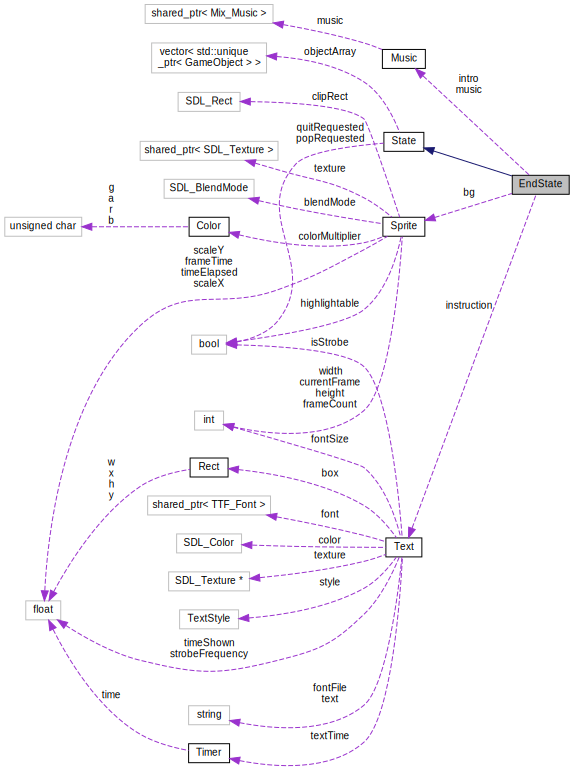
\includegraphics[width=350pt]{classEndState__coll__graph}
\end{center}
\end{figure}
\subsection*{Métodos Públicos}
\begin{DoxyCompactItemize}
\item 
\hyperlink{classEndState_a14303ccf71d755d28f5a0e79f40c69b4}{End\+State} (\hyperlink{classEndStateData}{End\+State\+Data} state\+Data)
\item 
void \hyperlink{classEndState_a0fabb275706a8324521ed1e88efda11d}{Update} (float dt)
\item 
void \hyperlink{classEndState_a1c876f3d062547988ac482f9c84d4b14}{Render} () const 
\item 
void \hyperlink{classEndState_ac0cc5426e529a4d8572b38e8a87d2d3e}{Pause} ()
\item 
void \hyperlink{classEndState_a27e54374f84da806d7bd8bfc985d41b9}{Resume} ()
\end{DoxyCompactItemize}
\subsection*{Atributos Privados}
\begin{DoxyCompactItemize}
\item 
\hyperlink{classSprite}{Sprite} \hyperlink{classEndState_aeb91899a27b89589e22685a888d4ba0a}{bg}
\item 
\hyperlink{classMusic}{Music} \hyperlink{classEndState_ad053a1cc844baf965edafc3607da6868}{music}
\item 
\hyperlink{classText}{Text} \hyperlink{classEndState_acbc4bcbbf722307b2ea222b5a85a0e8d}{instruction}
\end{DoxyCompactItemize}
\subsection*{Additional Inherited Members}


\subsection{Construtores \& Destrutores}
\hypertarget{classEndState_a14303ccf71d755d28f5a0e79f40c69b4}{\index{End\+State@{End\+State}!End\+State@{End\+State}}
\index{End\+State@{End\+State}!End\+State@{End\+State}}
\subsubsection[{End\+State}]{\setlength{\rightskip}{0pt plus 5cm}End\+State\+::\+End\+State (
\begin{DoxyParamCaption}
\item[{{\bf End\+State\+Data}}]{state\+Data}
\end{DoxyParamCaption}
)}}\label{classEndState_a14303ccf71d755d28f5a0e79f40c69b4}


\subsection{Métodos}
\hypertarget{classEndState_ac0cc5426e529a4d8572b38e8a87d2d3e}{\index{End\+State@{End\+State}!Pause@{Pause}}
\index{Pause@{Pause}!End\+State@{End\+State}}
\subsubsection[{Pause}]{\setlength{\rightskip}{0pt plus 5cm}void End\+State\+::\+Pause (
\begin{DoxyParamCaption}
\item[{void}]{}
\end{DoxyParamCaption}
)\hspace{0.3cm}{\ttfamily [virtual]}}}\label{classEndState_ac0cc5426e529a4d8572b38e8a87d2d3e}


Implementa \hyperlink{classState_ae9fa377b30f06fdd809a1557bfbc190a}{State}.

\hypertarget{classEndState_a1c876f3d062547988ac482f9c84d4b14}{\index{End\+State@{End\+State}!Render@{Render}}
\index{Render@{Render}!End\+State@{End\+State}}
\subsubsection[{Render}]{\setlength{\rightskip}{0pt plus 5cm}void End\+State\+::\+Render (
\begin{DoxyParamCaption}
\item[{void}]{}
\end{DoxyParamCaption}
) const\hspace{0.3cm}{\ttfamily [virtual]}}}\label{classEndState_a1c876f3d062547988ac482f9c84d4b14}


Implementa \hyperlink{classState_ad1f023e61676d0cef92afbaba48ec7ca}{State}.

\hypertarget{classEndState_a27e54374f84da806d7bd8bfc985d41b9}{\index{End\+State@{End\+State}!Resume@{Resume}}
\index{Resume@{Resume}!End\+State@{End\+State}}
\subsubsection[{Resume}]{\setlength{\rightskip}{0pt plus 5cm}void End\+State\+::\+Resume (
\begin{DoxyParamCaption}
\item[{void}]{}
\end{DoxyParamCaption}
)\hspace{0.3cm}{\ttfamily [virtual]}}}\label{classEndState_a27e54374f84da806d7bd8bfc985d41b9}


Implementa \hyperlink{classState_ac6d3f8b50530eec89e1344bab93f1006}{State}.

\hypertarget{classEndState_a0fabb275706a8324521ed1e88efda11d}{\index{End\+State@{End\+State}!Update@{Update}}
\index{Update@{Update}!End\+State@{End\+State}}
\subsubsection[{Update}]{\setlength{\rightskip}{0pt plus 5cm}void End\+State\+::\+Update (
\begin{DoxyParamCaption}
\item[{float}]{dt}
\end{DoxyParamCaption}
)\hspace{0.3cm}{\ttfamily [virtual]}}}\label{classEndState_a0fabb275706a8324521ed1e88efda11d}


Implementa \hyperlink{classState_ad79561dfb4e1a6b722a3d9c84b06e91c}{State}.



\subsection{Atributos}
\hypertarget{classEndState_aeb91899a27b89589e22685a888d4ba0a}{\index{End\+State@{End\+State}!bg@{bg}}
\index{bg@{bg}!End\+State@{End\+State}}
\subsubsection[{bg}]{\setlength{\rightskip}{0pt plus 5cm}{\bf Sprite} End\+State\+::bg\hspace{0.3cm}{\ttfamily [private]}}}\label{classEndState_aeb91899a27b89589e22685a888d4ba0a}
\hypertarget{classEndState_acbc4bcbbf722307b2ea222b5a85a0e8d}{\index{End\+State@{End\+State}!instruction@{instruction}}
\index{instruction@{instruction}!End\+State@{End\+State}}
\subsubsection[{instruction}]{\setlength{\rightskip}{0pt plus 5cm}{\bf Text} End\+State\+::instruction\hspace{0.3cm}{\ttfamily [private]}}}\label{classEndState_acbc4bcbbf722307b2ea222b5a85a0e8d}
\hypertarget{classEndState_ad053a1cc844baf965edafc3607da6868}{\index{End\+State@{End\+State}!music@{music}}
\index{music@{music}!End\+State@{End\+State}}
\subsubsection[{music}]{\setlength{\rightskip}{0pt plus 5cm}{\bf Music} End\+State\+::music\hspace{0.3cm}{\ttfamily [private]}}}\label{classEndState_ad053a1cc844baf965edafc3607da6868}


A documentação para esta classe foi gerada a partir dos seguintes arquivos\+:\begin{DoxyCompactItemize}
\item 
Game/include/\hyperlink{EndState_8h}{End\+State.\+h}\item 
Game/src/\hyperlink{EndState_8cpp}{End\+State.\+cpp}\end{DoxyCompactItemize}

\hypertarget{classEndStateData}{\section{Referência da Classe End\+State\+Data}
\label{classEndStateData}\index{End\+State\+Data@{End\+State\+Data}}
}


{\ttfamily \#include $<$End\+State\+Data.\+h$>$}



Diagrama de Hierarquia para End\+State\+Data\+:\nopagebreak
\begin{figure}[H]
\begin{center}
\leavevmode
\includegraphics[width=158pt]{classEndStateData__inherit__graph}
\end{center}
\end{figure}


Diagrama de colaboração para End\+State\+Data\+:\nopagebreak
\begin{figure}[H]
\begin{center}
\leavevmode
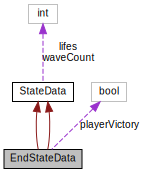
\includegraphics[width=216pt]{classEndStateData__coll__graph}
\end{center}
\end{figure}
\subsection*{Métodos Públicos}
\begin{DoxyCompactItemize}
\item 
bool \hyperlink{classEndStateData_abce01a73395040307914a4aa62741463}{Is} (\hyperlink{StateData_8h_a11e85d0fc3db733c13a8d9d030471c7d}{State\+Data\+Type} type\+To\+Check) const 
\item 
\hyperlink{classEndStateData_a3193e460f24f5cbd1098030864c75ddc}{End\+State\+Data} (bool \hyperlink{classEndStateData_aa26994b44ccac743a141c9709c526302}{player\+Victory})
\item 
bool \hyperlink{classEndStateData_abce01a73395040307914a4aa62741463}{Is} (\hyperlink{StateData_8h_a11e85d0fc3db733c13a8d9d030471c7d}{State\+Data\+Type} type\+To\+Check) const 
\item 
\hyperlink{classEndStateData_a3193e460f24f5cbd1098030864c75ddc}{End\+State\+Data} (bool \hyperlink{classEndStateData_aa26994b44ccac743a141c9709c526302}{player\+Victory})
\end{DoxyCompactItemize}
\subsection*{Atributos Públicos}
\begin{DoxyCompactItemize}
\item 
bool \hyperlink{classEndStateData_aa26994b44ccac743a141c9709c526302}{player\+Victory}
\end{DoxyCompactItemize}
\subsection*{Additional Inherited Members}


\subsection{Construtores \& Destrutores}
\hypertarget{classEndStateData_a3193e460f24f5cbd1098030864c75ddc}{\index{End\+State\+Data@{End\+State\+Data}!End\+State\+Data@{End\+State\+Data}}
\index{End\+State\+Data@{End\+State\+Data}!End\+State\+Data@{End\+State\+Data}}
\subsubsection[{End\+State\+Data}]{\setlength{\rightskip}{0pt plus 5cm}End\+State\+Data\+::\+End\+State\+Data (
\begin{DoxyParamCaption}
\item[{bool}]{player\+Victory}
\end{DoxyParamCaption}
)\hspace{0.3cm}{\ttfamily [inline]}}}\label{classEndStateData_a3193e460f24f5cbd1098030864c75ddc}
\hypertarget{classEndStateData_a3193e460f24f5cbd1098030864c75ddc}{\index{End\+State\+Data@{End\+State\+Data}!End\+State\+Data@{End\+State\+Data}}
\index{End\+State\+Data@{End\+State\+Data}!End\+State\+Data@{End\+State\+Data}}
\subsubsection[{End\+State\+Data}]{\setlength{\rightskip}{0pt plus 5cm}End\+State\+Data\+::\+End\+State\+Data (
\begin{DoxyParamCaption}
\item[{bool}]{player\+Victory}
\end{DoxyParamCaption}
)}}\label{classEndStateData_a3193e460f24f5cbd1098030864c75ddc}


\subsection{Métodos}
\hypertarget{classEndStateData_abce01a73395040307914a4aa62741463}{\index{End\+State\+Data@{End\+State\+Data}!Is@{Is}}
\index{Is@{Is}!End\+State\+Data@{End\+State\+Data}}
\subsubsection[{Is}]{\setlength{\rightskip}{0pt plus 5cm}bool End\+State\+Data\+::\+Is (
\begin{DoxyParamCaption}
\item[{{\bf State\+Data\+Type}}]{type\+To\+Check}
\end{DoxyParamCaption}
) const\hspace{0.3cm}{\ttfamily [inline]}, {\ttfamily [virtual]}}}\label{classEndStateData_abce01a73395040307914a4aa62741463}


Implementa \hyperlink{classStateData_a63b33546d704a06bf8f9df6b0590eae4}{State\+Data}.

\hypertarget{classEndStateData_abce01a73395040307914a4aa62741463}{\index{End\+State\+Data@{End\+State\+Data}!Is@{Is}}
\index{Is@{Is}!End\+State\+Data@{End\+State\+Data}}
\subsubsection[{Is}]{\setlength{\rightskip}{0pt plus 5cm}bool End\+State\+Data\+::\+Is (
\begin{DoxyParamCaption}
\item[{{\bf State\+Data\+Type}}]{type\+To\+Check}
\end{DoxyParamCaption}
) const\hspace{0.3cm}{\ttfamily [virtual]}}}\label{classEndStateData_abce01a73395040307914a4aa62741463}


Implementa \hyperlink{classStateData_a63b33546d704a06bf8f9df6b0590eae4}{State\+Data}.



\subsection{Atributos}
\hypertarget{classEndStateData_aa26994b44ccac743a141c9709c526302}{\index{End\+State\+Data@{End\+State\+Data}!player\+Victory@{player\+Victory}}
\index{player\+Victory@{player\+Victory}!End\+State\+Data@{End\+State\+Data}}
\subsubsection[{player\+Victory}]{\setlength{\rightskip}{0pt plus 5cm}bool End\+State\+Data\+::player\+Victory}}\label{classEndStateData_aa26994b44ccac743a141c9709c526302}


A documentação para esta classe foi gerada a partir dos seguintes arquivos\+:\begin{DoxyCompactItemize}
\item 
Game/include/\hyperlink{EndStateData_8h}{End\+State\+Data.\+h}\item 
Game/src/\hyperlink{EndStateData_8cpp}{End\+State\+Data.\+cpp}\end{DoxyCompactItemize}

\hypertarget{classGame}{\section{Referência da Classe Game}
\label{classGame}\index{Game@{Game}}
}


{\ttfamily \#include $<$Game.\+h$>$}



Diagrama de colaboração para Game\+:\nopagebreak
\begin{figure}[H]
\begin{center}
\leavevmode
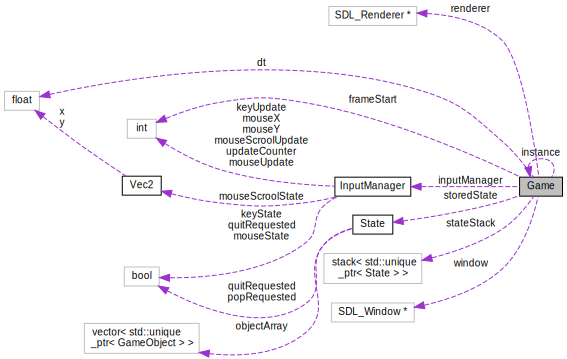
\includegraphics[width=350pt]{classGame__coll__graph}
\end{center}
\end{figure}
\subsection*{Métodos Públicos}
\begin{DoxyCompactItemize}
\item 
\hyperlink{classGame_acf1ee7a59d78a51832e8878cfca81c5a}{Game} (std\+::string title, int width, int height)
\item 
\hyperlink{classGame_ae3d112ca6e0e55150d2fdbc704474530}{$\sim$\+Game} ()
\item 
S\+D\+L\+\_\+\+Renderer $\ast$ \hyperlink{classGame_a5749c6fc2bf3c98a4dc9c11e33f96c8b}{Get\+Renderer} (void) const 
\item 
\hyperlink{classState}{State} \& \hyperlink{classGame_a1f9d6f97e969424844881dd7ad2e353e}{Get\+Current\+State} (void) const 
\item 
void \hyperlink{classGame_ab5637c16d9580f8ec08b5830baff35bd}{Push} (\hyperlink{classState}{State} $\ast$state)
\item 
void \hyperlink{classGame_a7415a437ef79fd22feb4d26f714f9c0f}{Run} (void)
\item 
float \hyperlink{classGame_aa2feacb19b45ff0ec0935ea1a6f9c9ab}{Get\+Delta\+Time} (void) const 
\item 
\hyperlink{classVec2}{Vec2} \hyperlink{classGame_adbeb87bbabcc73f936e149c2d83d9d33}{Get\+Window\+Dimensions} (void) const 
\end{DoxyCompactItemize}
\subsection*{Métodos Públicos Estáticos}
\begin{DoxyCompactItemize}
\item 
static \hyperlink{classGame}{Game} \& \hyperlink{classGame_a25d213802ed39215e3ab2cb04edf46c8}{Get\+Instance} (void)
\end{DoxyCompactItemize}
\subsection*{Métodos Privados}
\begin{DoxyCompactItemize}
\item 
void \hyperlink{classGame_afddce07e3e3d3ca05a6c2f2ca9e64940}{Calculate\+Delta\+Time} (void)
\item 
void \hyperlink{classGame_ae67b3fda973e4b05513d02c968b0ac17}{Update\+Stack} (void)
\end{DoxyCompactItemize}
\subsection*{Atributos Privados}
\begin{DoxyCompactItemize}
\item 
unsigned int \hyperlink{classGame_af21b5344d8b7796d5f425bdbe37a6c82}{frame\+Start}
\item 
float \hyperlink{classGame_a5184b0439c5cefb45050d0bfaca9ac97}{dt}
\item 
\hyperlink{classState}{State} $\ast$ \hyperlink{classGame_a46a38cae75b6557890d7c47ad8350a1d}{stored\+State}
\item 
S\+D\+L\+\_\+\+Window $\ast$ \hyperlink{classGame_adc376cc3011b5c8f1c3897626100174c}{window}
\item 
S\+D\+L\+\_\+\+Renderer $\ast$ \hyperlink{classGame_ae5164c37c0dc74cfb56041174017bf57}{renderer}
\item 
std\+::stack$<$ std\+::unique\+\_\+ptr\\*
$<$ \hyperlink{classState}{State} $>$ $>$ \hyperlink{classGame_a2706caaad0c60784a6671efc9ee147f8}{state\+Stack}
\item 
\hyperlink{classInputManager}{Input\+Manager} \& \hyperlink{classGame_a57010b9ce85884e0f4059d8d8474e610}{input\+Manager}
\end{DoxyCompactItemize}
\subsection*{Atributos Privados Estáticos}
\begin{DoxyCompactItemize}
\item 
static \hyperlink{classGame}{Game} $\ast$ \hyperlink{classGame_aa469cdc0a30f4fd2d6d99b23f4fbf257}{instance} = nullptr
\end{DoxyCompactItemize}


\subsection{Construtores \& Destrutores}
\hypertarget{classGame_acf1ee7a59d78a51832e8878cfca81c5a}{\index{Game@{Game}!Game@{Game}}
\index{Game@{Game}!Game@{Game}}
\subsubsection[{Game}]{\setlength{\rightskip}{0pt plus 5cm}Game\+::\+Game (
\begin{DoxyParamCaption}
\item[{std\+::string}]{title, }
\item[{int}]{width, }
\item[{int}]{height}
\end{DoxyParamCaption}
)}}\label{classGame_acf1ee7a59d78a51832e8878cfca81c5a}
\hypertarget{classGame_ae3d112ca6e0e55150d2fdbc704474530}{\index{Game@{Game}!````~Game@{$\sim$\+Game}}
\index{````~Game@{$\sim$\+Game}!Game@{Game}}
\subsubsection[{$\sim$\+Game}]{\setlength{\rightskip}{0pt plus 5cm}Game\+::$\sim$\+Game (
\begin{DoxyParamCaption}
{}
\end{DoxyParamCaption}
)}}\label{classGame_ae3d112ca6e0e55150d2fdbc704474530}


\subsection{Métodos}
\hypertarget{classGame_afddce07e3e3d3ca05a6c2f2ca9e64940}{\index{Game@{Game}!Calculate\+Delta\+Time@{Calculate\+Delta\+Time}}
\index{Calculate\+Delta\+Time@{Calculate\+Delta\+Time}!Game@{Game}}
\subsubsection[{Calculate\+Delta\+Time}]{\setlength{\rightskip}{0pt plus 5cm}void Game\+::\+Calculate\+Delta\+Time (
\begin{DoxyParamCaption}
\item[{void}]{}
\end{DoxyParamCaption}
)\hspace{0.3cm}{\ttfamily [private]}}}\label{classGame_afddce07e3e3d3ca05a6c2f2ca9e64940}
\hypertarget{classGame_a1f9d6f97e969424844881dd7ad2e353e}{\index{Game@{Game}!Get\+Current\+State@{Get\+Current\+State}}
\index{Get\+Current\+State@{Get\+Current\+State}!Game@{Game}}
\subsubsection[{Get\+Current\+State}]{\setlength{\rightskip}{0pt plus 5cm}{\bf State} \& Game\+::\+Get\+Current\+State (
\begin{DoxyParamCaption}
\item[{void}]{}
\end{DoxyParamCaption}
) const}}\label{classGame_a1f9d6f97e969424844881dd7ad2e353e}
\hypertarget{classGame_aa2feacb19b45ff0ec0935ea1a6f9c9ab}{\index{Game@{Game}!Get\+Delta\+Time@{Get\+Delta\+Time}}
\index{Get\+Delta\+Time@{Get\+Delta\+Time}!Game@{Game}}
\subsubsection[{Get\+Delta\+Time}]{\setlength{\rightskip}{0pt plus 5cm}float Game\+::\+Get\+Delta\+Time (
\begin{DoxyParamCaption}
\item[{void}]{}
\end{DoxyParamCaption}
) const}}\label{classGame_aa2feacb19b45ff0ec0935ea1a6f9c9ab}
\hypertarget{classGame_a25d213802ed39215e3ab2cb04edf46c8}{\index{Game@{Game}!Get\+Instance@{Get\+Instance}}
\index{Get\+Instance@{Get\+Instance}!Game@{Game}}
\subsubsection[{Get\+Instance}]{\setlength{\rightskip}{0pt plus 5cm}{\bf Game} \& Game\+::\+Get\+Instance (
\begin{DoxyParamCaption}
\item[{void}]{}
\end{DoxyParamCaption}
)\hspace{0.3cm}{\ttfamily [static]}}}\label{classGame_a25d213802ed39215e3ab2cb04edf46c8}
\hypertarget{classGame_a5749c6fc2bf3c98a4dc9c11e33f96c8b}{\index{Game@{Game}!Get\+Renderer@{Get\+Renderer}}
\index{Get\+Renderer@{Get\+Renderer}!Game@{Game}}
\subsubsection[{Get\+Renderer}]{\setlength{\rightskip}{0pt plus 5cm}S\+D\+L\+\_\+\+Renderer $\ast$ Game\+::\+Get\+Renderer (
\begin{DoxyParamCaption}
\item[{void}]{}
\end{DoxyParamCaption}
) const}}\label{classGame_a5749c6fc2bf3c98a4dc9c11e33f96c8b}
\hypertarget{classGame_adbeb87bbabcc73f936e149c2d83d9d33}{\index{Game@{Game}!Get\+Window\+Dimensions@{Get\+Window\+Dimensions}}
\index{Get\+Window\+Dimensions@{Get\+Window\+Dimensions}!Game@{Game}}
\subsubsection[{Get\+Window\+Dimensions}]{\setlength{\rightskip}{0pt plus 5cm}{\bf Vec2} Game\+::\+Get\+Window\+Dimensions (
\begin{DoxyParamCaption}
\item[{void}]{}
\end{DoxyParamCaption}
) const}}\label{classGame_adbeb87bbabcc73f936e149c2d83d9d33}
\hypertarget{classGame_ab5637c16d9580f8ec08b5830baff35bd}{\index{Game@{Game}!Push@{Push}}
\index{Push@{Push}!Game@{Game}}
\subsubsection[{Push}]{\setlength{\rightskip}{0pt plus 5cm}void Game\+::\+Push (
\begin{DoxyParamCaption}
\item[{{\bf State} $\ast$}]{state}
\end{DoxyParamCaption}
)}}\label{classGame_ab5637c16d9580f8ec08b5830baff35bd}
\hypertarget{classGame_a7415a437ef79fd22feb4d26f714f9c0f}{\index{Game@{Game}!Run@{Run}}
\index{Run@{Run}!Game@{Game}}
\subsubsection[{Run}]{\setlength{\rightskip}{0pt plus 5cm}void Game\+::\+Run (
\begin{DoxyParamCaption}
\item[{void}]{}
\end{DoxyParamCaption}
)}}\label{classGame_a7415a437ef79fd22feb4d26f714f9c0f}
\hypertarget{classGame_ae67b3fda973e4b05513d02c968b0ac17}{\index{Game@{Game}!Update\+Stack@{Update\+Stack}}
\index{Update\+Stack@{Update\+Stack}!Game@{Game}}
\subsubsection[{Update\+Stack}]{\setlength{\rightskip}{0pt plus 5cm}void Game\+::\+Update\+Stack (
\begin{DoxyParamCaption}
\item[{void}]{}
\end{DoxyParamCaption}
)\hspace{0.3cm}{\ttfamily [private]}}}\label{classGame_ae67b3fda973e4b05513d02c968b0ac17}


\subsection{Atributos}
\hypertarget{classGame_a5184b0439c5cefb45050d0bfaca9ac97}{\index{Game@{Game}!dt@{dt}}
\index{dt@{dt}!Game@{Game}}
\subsubsection[{dt}]{\setlength{\rightskip}{0pt plus 5cm}float Game\+::dt\hspace{0.3cm}{\ttfamily [private]}}}\label{classGame_a5184b0439c5cefb45050d0bfaca9ac97}
\hypertarget{classGame_af21b5344d8b7796d5f425bdbe37a6c82}{\index{Game@{Game}!frame\+Start@{frame\+Start}}
\index{frame\+Start@{frame\+Start}!Game@{Game}}
\subsubsection[{frame\+Start}]{\setlength{\rightskip}{0pt plus 5cm}unsigned int Game\+::frame\+Start\hspace{0.3cm}{\ttfamily [private]}}}\label{classGame_af21b5344d8b7796d5f425bdbe37a6c82}
\hypertarget{classGame_a57010b9ce85884e0f4059d8d8474e610}{\index{Game@{Game}!input\+Manager@{input\+Manager}}
\index{input\+Manager@{input\+Manager}!Game@{Game}}
\subsubsection[{input\+Manager}]{\setlength{\rightskip}{0pt plus 5cm}{\bf Input\+Manager}\& Game\+::input\+Manager\hspace{0.3cm}{\ttfamily [private]}}}\label{classGame_a57010b9ce85884e0f4059d8d8474e610}
\hypertarget{classGame_aa469cdc0a30f4fd2d6d99b23f4fbf257}{\index{Game@{Game}!instance@{instance}}
\index{instance@{instance}!Game@{Game}}
\subsubsection[{instance}]{\setlength{\rightskip}{0pt plus 5cm}{\bf Game} $\ast$ Game\+::instance = nullptr\hspace{0.3cm}{\ttfamily [static]}, {\ttfamily [private]}}}\label{classGame_aa469cdc0a30f4fd2d6d99b23f4fbf257}
\hypertarget{classGame_ae5164c37c0dc74cfb56041174017bf57}{\index{Game@{Game}!renderer@{renderer}}
\index{renderer@{renderer}!Game@{Game}}
\subsubsection[{renderer}]{\setlength{\rightskip}{0pt plus 5cm}S\+D\+L\+\_\+\+Renderer$\ast$ Game\+::renderer\hspace{0.3cm}{\ttfamily [private]}}}\label{classGame_ae5164c37c0dc74cfb56041174017bf57}
\hypertarget{classGame_a2706caaad0c60784a6671efc9ee147f8}{\index{Game@{Game}!state\+Stack@{state\+Stack}}
\index{state\+Stack@{state\+Stack}!Game@{Game}}
\subsubsection[{state\+Stack}]{\setlength{\rightskip}{0pt plus 5cm}std\+::stack$<$std\+::unique\+\_\+ptr$<${\bf State}$>$ $>$ Game\+::state\+Stack\hspace{0.3cm}{\ttfamily [private]}}}\label{classGame_a2706caaad0c60784a6671efc9ee147f8}
\hypertarget{classGame_a46a38cae75b6557890d7c47ad8350a1d}{\index{Game@{Game}!stored\+State@{stored\+State}}
\index{stored\+State@{stored\+State}!Game@{Game}}
\subsubsection[{stored\+State}]{\setlength{\rightskip}{0pt plus 5cm}{\bf State}$\ast$ Game\+::stored\+State\hspace{0.3cm}{\ttfamily [private]}}}\label{classGame_a46a38cae75b6557890d7c47ad8350a1d}
\hypertarget{classGame_adc376cc3011b5c8f1c3897626100174c}{\index{Game@{Game}!window@{window}}
\index{window@{window}!Game@{Game}}
\subsubsection[{window}]{\setlength{\rightskip}{0pt plus 5cm}S\+D\+L\+\_\+\+Window$\ast$ Game\+::window\hspace{0.3cm}{\ttfamily [private]}}}\label{classGame_adc376cc3011b5c8f1c3897626100174c}


A documentação para esta classe foi gerada a partir dos seguintes arquivos\+:\begin{DoxyCompactItemize}
\item 
Engine/include/\hyperlink{Game_8h}{Game.\+h}\item 
Engine/src/\hyperlink{Game_8cpp}{Game.\+cpp}\end{DoxyCompactItemize}

\hypertarget{classGameObject}{\section{Referência da Classe Game\+Object}
\label{classGameObject}\index{Game\+Object@{Game\+Object}}
}


{\ttfamily \#include $<$Gameobject.\+h$>$}



Diagrama de Hierarquia para Game\+Object\+:\nopagebreak
\begin{figure}[H]
\begin{center}
\leavevmode
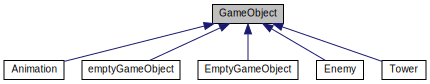
\includegraphics[width=350pt]{classGameObject__inherit__graph}
\end{center}
\end{figure}


Diagrama de colaboração para Game\+Object\+:\nopagebreak
\begin{figure}[H]
\begin{center}
\leavevmode
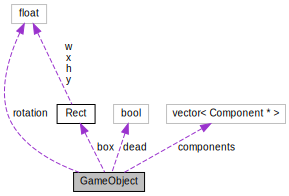
\includegraphics[width=182pt]{classGameObject__coll__graph}
\end{center}
\end{figure}
\subsection*{Métodos Públicos}
\begin{DoxyCompactItemize}
\item 
\hyperlink{classGameObject_a78da814b13c8bf344ba0c5f72cb22af3}{Game\+Object} (void)
\item 
virtual \hyperlink{classGameObject_a3b086987a48c14ebe80939bd66d5f1c8}{$\sim$\+Game\+Object} (void)
\item 
virtual void \hyperlink{classGameObject_a93ed63df640deb516a020530e7f8e045}{Update} (float dt)=0
\item 
virtual void \hyperlink{classGameObject_a976b9c0d72212389603802f95b3f3424}{Render} (void)=0
\item 
virtual bool \hyperlink{classGameObject_a076afa2ea9190c49046f86a0946b4543}{Is\+Dead} (void)=0
\item 
virtual void \hyperlink{classGameObject_aa627e6c2913983fc5f108c1c4d303eb8}{Notify\+Collision} (\hyperlink{classGameObject}{Game\+Object} \&other)=0
\item 
virtual bool \hyperlink{classGameObject_a3ddba599a800d774463c7082b7ef4801}{Is} (string type)=0
\end{DoxyCompactItemize}
\subsection*{Atributos Públicos}
\begin{DoxyCompactItemize}
\item 
\hyperlink{classRect}{Rect} \hyperlink{classGameObject_ac8df90f2a6d41693cd7938e392ff6d0b}{box}
\item 
float \hyperlink{classGameObject_ac55f6ebdf4cfbab508680ad7290fb26c}{rotation}
\end{DoxyCompactItemize}


\subsection{Construtores \& Destrutores}
\hypertarget{classGameObject_a78da814b13c8bf344ba0c5f72cb22af3}{\index{Game\+Object@{Game\+Object}!Game\+Object@{Game\+Object}}
\index{Game\+Object@{Game\+Object}!Game\+Object@{Game\+Object}}
\subsubsection[{Game\+Object}]{\setlength{\rightskip}{0pt plus 5cm}Game\+Object\+::\+Game\+Object (
\begin{DoxyParamCaption}
\item[{void}]{}
\end{DoxyParamCaption}
)}}\label{classGameObject_a78da814b13c8bf344ba0c5f72cb22af3}
\hypertarget{classGameObject_a3b086987a48c14ebe80939bd66d5f1c8}{\index{Game\+Object@{Game\+Object}!````~Game\+Object@{$\sim$\+Game\+Object}}
\index{````~Game\+Object@{$\sim$\+Game\+Object}!Game\+Object@{Game\+Object}}
\subsubsection[{$\sim$\+Game\+Object}]{\setlength{\rightskip}{0pt plus 5cm}Game\+Object\+::$\sim$\+Game\+Object (
\begin{DoxyParamCaption}
\item[{void}]{}
\end{DoxyParamCaption}
)\hspace{0.3cm}{\ttfamily [virtual]}}}\label{classGameObject_a3b086987a48c14ebe80939bd66d5f1c8}


\subsection{Métodos}
\hypertarget{classGameObject_a3ddba599a800d774463c7082b7ef4801}{\index{Game\+Object@{Game\+Object}!Is@{Is}}
\index{Is@{Is}!Game\+Object@{Game\+Object}}
\subsubsection[{Is}]{\setlength{\rightskip}{0pt plus 5cm}virtual bool Game\+Object\+::\+Is (
\begin{DoxyParamCaption}
\item[{string}]{type}
\end{DoxyParamCaption}
)\hspace{0.3cm}{\ttfamily [pure virtual]}}}\label{classGameObject_a3ddba599a800d774463c7082b7ef4801}


Implementado por \hyperlink{classBullet_aaa159cc9dcc3e7c780bbccc1ebc6d95a}{Bullet}, \hyperlink{classAlien_a9697e1dc132cc829d787c8bd586a01a2}{Alien}, \hyperlink{classAnimation_a166f36012f3092275648a74272e8ff0f}{Animation}, \hyperlink{classPenguins_a73a0c4f96de975d6219b4d6016fac29e}{Penguins} e \hyperlink{classMinion_a27b0afce19e3ab3e4c76615d5902207e}{Minion}.

\hypertarget{classGameObject_a076afa2ea9190c49046f86a0946b4543}{\index{Game\+Object@{Game\+Object}!Is\+Dead@{Is\+Dead}}
\index{Is\+Dead@{Is\+Dead}!Game\+Object@{Game\+Object}}
\subsubsection[{Is\+Dead}]{\setlength{\rightskip}{0pt plus 5cm}virtual bool Game\+Object\+::\+Is\+Dead (
\begin{DoxyParamCaption}
\item[{void}]{}
\end{DoxyParamCaption}
)\hspace{0.3cm}{\ttfamily [pure virtual]}}}\label{classGameObject_a076afa2ea9190c49046f86a0946b4543}


Implementado por \hyperlink{classBullet_a17cf15fdfa0c42931f21828feed2a77d}{Bullet}, \hyperlink{classAlien_a27d2042c7097c2d37bb0268575ec8bad}{Alien}, \hyperlink{classAnimation_ad1eaa9ff240cbcc114270ea174523702}{Animation}, \hyperlink{classPenguins_ab76c07904df3da2d768f08eb3da3d1e0}{Penguins} e \hyperlink{classMinion_a9743cf683c7860011c56523818cc14cb}{Minion}.

\hypertarget{classGameObject_aa627e6c2913983fc5f108c1c4d303eb8}{\index{Game\+Object@{Game\+Object}!Notify\+Collision@{Notify\+Collision}}
\index{Notify\+Collision@{Notify\+Collision}!Game\+Object@{Game\+Object}}
\subsubsection[{Notify\+Collision}]{\setlength{\rightskip}{0pt plus 5cm}virtual void Game\+Object\+::\+Notify\+Collision (
\begin{DoxyParamCaption}
\item[{{\bf Game\+Object} \&}]{other}
\end{DoxyParamCaption}
)\hspace{0.3cm}{\ttfamily [pure virtual]}}}\label{classGameObject_aa627e6c2913983fc5f108c1c4d303eb8}


Implementado por \hyperlink{classBullet_a272c1b019f46df9ad9bd45bd9ffb6e41}{Bullet}, \hyperlink{classAlien_a47baef9f1b44ad393b268812b752bd3a}{Alien}, \hyperlink{classAnimation_a611b21418311eb697ec4af1aaff92657}{Animation}, \hyperlink{classPenguins_aba0e8bc9309f056d196cd0fd267fbe78}{Penguins} e \hyperlink{classMinion_a908a2d009bad951df8bfd40067074059}{Minion}.

\hypertarget{classGameObject_a976b9c0d72212389603802f95b3f3424}{\index{Game\+Object@{Game\+Object}!Render@{Render}}
\index{Render@{Render}!Game\+Object@{Game\+Object}}
\subsubsection[{Render}]{\setlength{\rightskip}{0pt plus 5cm}virtual void Game\+Object\+::\+Render (
\begin{DoxyParamCaption}
\item[{void}]{}
\end{DoxyParamCaption}
)\hspace{0.3cm}{\ttfamily [pure virtual]}}}\label{classGameObject_a976b9c0d72212389603802f95b3f3424}


Implementado por \hyperlink{classBullet_aace1e49986271afb6384d15bf40a0e92}{Bullet}, \hyperlink{classAlien_a43e7b457eb4f8c41deae1a37aaf8622c}{Alien}, \hyperlink{classAnimation_a49749e3890cec3896e6f726323544c26}{Animation}, \hyperlink{classPenguins_a5af1c983add97265c7491d17d2dc019e}{Penguins} e \hyperlink{classMinion_af62874486a43cd5d4ecc84d9361c58dc}{Minion}.

\hypertarget{classGameObject_a93ed63df640deb516a020530e7f8e045}{\index{Game\+Object@{Game\+Object}!Update@{Update}}
\index{Update@{Update}!Game\+Object@{Game\+Object}}
\subsubsection[{Update}]{\setlength{\rightskip}{0pt plus 5cm}virtual void Game\+Object\+::\+Update (
\begin{DoxyParamCaption}
\item[{float}]{dt}
\end{DoxyParamCaption}
)\hspace{0.3cm}{\ttfamily [pure virtual]}}}\label{classGameObject_a93ed63df640deb516a020530e7f8e045}


Implementado por \hyperlink{classBullet_a5ca74d7990f25c518df1860b681079ea}{Bullet}, \hyperlink{classAlien_a5bcca286b1a9d8f3fc56a2e8d5636b19}{Alien}, \hyperlink{classAnimation_a1871db60d1fb351aeb77ada38dd4dd9c}{Animation}, \hyperlink{classPenguins_a63b378e640cd3a76cbe6afaf0c6578d7}{Penguins} e \hyperlink{classMinion_a5a9a53136ca0ee5fd5766410ff9acaa6}{Minion}.



\subsection{Atributos}
\hypertarget{classGameObject_ac8df90f2a6d41693cd7938e392ff6d0b}{\index{Game\+Object@{Game\+Object}!box@{box}}
\index{box@{box}!Game\+Object@{Game\+Object}}
\subsubsection[{box}]{\setlength{\rightskip}{0pt plus 5cm}{\bf Rect} Game\+Object\+::box}}\label{classGameObject_ac8df90f2a6d41693cd7938e392ff6d0b}
\hypertarget{classGameObject_ac55f6ebdf4cfbab508680ad7290fb26c}{\index{Game\+Object@{Game\+Object}!rotation@{rotation}}
\index{rotation@{rotation}!Game\+Object@{Game\+Object}}
\subsubsection[{rotation}]{\setlength{\rightskip}{0pt plus 5cm}float Game\+Object\+::rotation}}\label{classGameObject_ac55f6ebdf4cfbab508680ad7290fb26c}


A documentação para esta classe foi gerada a partir dos seguintes arquivos\+:\begin{DoxyCompactItemize}
\item 
Engine/include/\hyperlink{Gameobject_8h}{Gameobject.\+h}\item 
Engine/src/\hyperlink{Gameobject_8cpp}{Gameobject.\+cpp}\end{DoxyCompactItemize}

\hypertarget{classInputManager}{\section{Referência da Classe Input\+Manager}
\label{classInputManager}\index{Input\+Manager@{Input\+Manager}}
}


{\ttfamily \#include $<$Input\+Manager.\+h$>$}



Diagrama de colaboração para Input\+Manager\+:
\nopagebreak
\begin{figure}[H]
\begin{center}
\leavevmode
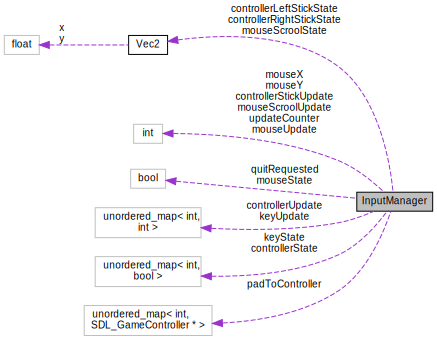
\includegraphics[width=350pt]{classInputManager__coll__graph}
\end{center}
\end{figure}
\subsection*{Métodos Públicos}
\begin{DoxyCompactItemize}
\item 
void \hyperlink{classInputManager_afc344b3b2e204cfb39ee17b33bcc5eab}{Update} (void)
\item 
bool \hyperlink{classInputManager_a6793bc63304cafeaf45151d083946f42}{Key\+Press} (int key) const 
\item 
bool \hyperlink{classInputManager_a161025491900d61e6090d6f6e576934f}{Key\+Release} (int key) const 
\item 
bool \hyperlink{classInputManager_a97d25d372ab28dbc119b5a0919e38244}{Is\+Key\+Down} (int key) const 
\item 
bool \hyperlink{classInputManager_ad07e913718fc94601dfccb5c3a6fb0ae}{Mouse\+Press} (int button) const 
\item 
bool \hyperlink{classInputManager_a0056b265c8790bf862f6bff283349985}{Mouse\+Release} (int button) const 
\item 
bool \hyperlink{classInputManager_a410c6f6a0fa13dfd938d6d26a524fc19}{Is\+Mouse\+Down} (int button) const 
\item 
bool \hyperlink{classInputManager_aeb81e9386db70d1cc204e45963ec9077}{Is\+Mouse\+Scrolling} (void) const 
\item 
int \hyperlink{classInputManager_aaa3f36152ef8fdec75c0e3f5307979fb}{Get\+Mouse\+X} (void) const 
\item 
int \hyperlink{classInputManager_a3883f6471f5d124fd51990af3fdff24d}{Get\+Mouse\+Y} (void) const 
\item 
\hyperlink{classVec2}{Vec2} \hyperlink{classInputManager_a8609a7850d6c037642539c19ab53a4e8}{Get\+Mouse\+Pos} (void) const 
\item 
\hyperlink{classVec2}{Vec2} \hyperlink{classInputManager_acfca74249b64db2cb2a3b67c0e944696}{Mouse\+Scroll} (void) const 
\item 
bool \hyperlink{classInputManager_a0c96a7ae70931d034a78a8e97b70dd27}{Quit\+Requested} (void) const 
\end{DoxyCompactItemize}
\subsection*{Métodos Públicos Estáticos}
\begin{DoxyCompactItemize}
\item 
static \hyperlink{classInputManager}{Input\+Manager} \& \hyperlink{classInputManager_a1f095ed502f0bd09390d05cdc0acdcd9}{Get\+Instance} (void)
\end{DoxyCompactItemize}
\subsection*{Métodos Privados}
\begin{DoxyCompactItemize}
\item 
\hyperlink{classInputManager_a8be46886da639b26d67181c29dab6d6c}{Input\+Manager} ()
\item 
\hyperlink{classInputManager_af518290877dd183606709d5852db5491}{$\sim$\+Input\+Manager} ()
\end{DoxyCompactItemize}
\subsection*{Atributos Privados}
\begin{DoxyCompactItemize}
\item 
bool \hyperlink{classInputManager_af0f48b36a7d8e0f2c0b24057143b29c7}{mouse\+State} \mbox{[}6\mbox{]}
\item 
int \hyperlink{classInputManager_a1226f8af91792ac5ac5adda5fa2f0db0}{mouse\+Update} \mbox{[}6\mbox{]}
\item 
bool \hyperlink{classInputManager_a078d1f2f8af5f17005f21f7407dbca57}{quit\+Requested}
\item 
int \hyperlink{classInputManager_a96541a9ebd43184f92449f9daf94724f}{update\+Counter}
\item 
int \hyperlink{classInputManager_a29fddcf9d741e4de04492ad76b7cb3af}{mouse\+X}
\item 
int \hyperlink{classInputManager_afb189c58dd5ee470a3202c685c5c7f1e}{mouse\+Y}
\item 
bool \hyperlink{classInputManager_a3c6b0a27b387bfb4b2fc669db0f68bad}{key\+State} \mbox{[}416\mbox{]}
\item 
int \hyperlink{classInputManager_ae8ce3bc2865693cbb548ef2f1603f991}{key\+Update} \mbox{[}416\mbox{]}
\item 
int \hyperlink{classInputManager_a646fc44d21853e1354aaacc6a27e79ca}{mouse\+Scrool\+Update}
\item 
\hyperlink{classVec2}{Vec2} \hyperlink{classInputManager_a9c9d5ed1da1b205d9311ec4a9bab06ea}{mouse\+Scrool\+State}
\end{DoxyCompactItemize}


\subsection{Construtores \& Destrutores}
\hypertarget{classInputManager_a8be46886da639b26d67181c29dab6d6c}{\index{Input\+Manager@{Input\+Manager}!Input\+Manager@{Input\+Manager}}
\index{Input\+Manager@{Input\+Manager}!Input\+Manager@{Input\+Manager}}
\subsubsection[{Input\+Manager}]{\setlength{\rightskip}{0pt plus 5cm}Input\+Manager\+::\+Input\+Manager (
\begin{DoxyParamCaption}
{}
\end{DoxyParamCaption}
)\hspace{0.3cm}{\ttfamily [private]}}}\label{classInputManager_a8be46886da639b26d67181c29dab6d6c}
\hypertarget{classInputManager_af518290877dd183606709d5852db5491}{\index{Input\+Manager@{Input\+Manager}!````~Input\+Manager@{$\sim$\+Input\+Manager}}
\index{````~Input\+Manager@{$\sim$\+Input\+Manager}!Input\+Manager@{Input\+Manager}}
\subsubsection[{$\sim$\+Input\+Manager}]{\setlength{\rightskip}{0pt plus 5cm}Input\+Manager\+::$\sim$\+Input\+Manager (
\begin{DoxyParamCaption}
{}
\end{DoxyParamCaption}
)\hspace{0.3cm}{\ttfamily [private]}}}\label{classInputManager_af518290877dd183606709d5852db5491}


\subsection{Métodos}
\hypertarget{classInputManager_a1f095ed502f0bd09390d05cdc0acdcd9}{\index{Input\+Manager@{Input\+Manager}!Get\+Instance@{Get\+Instance}}
\index{Get\+Instance@{Get\+Instance}!Input\+Manager@{Input\+Manager}}
\subsubsection[{Get\+Instance}]{\setlength{\rightskip}{0pt plus 5cm}{\bf Input\+Manager} \& Input\+Manager\+::\+Get\+Instance (
\begin{DoxyParamCaption}
\item[{void}]{}
\end{DoxyParamCaption}
)\hspace{0.3cm}{\ttfamily [static]}}}\label{classInputManager_a1f095ed502f0bd09390d05cdc0acdcd9}
\hypertarget{classInputManager_a8609a7850d6c037642539c19ab53a4e8}{\index{Input\+Manager@{Input\+Manager}!Get\+Mouse\+Pos@{Get\+Mouse\+Pos}}
\index{Get\+Mouse\+Pos@{Get\+Mouse\+Pos}!Input\+Manager@{Input\+Manager}}
\subsubsection[{Get\+Mouse\+Pos}]{\setlength{\rightskip}{0pt plus 5cm}{\bf Vec2} Input\+Manager\+::\+Get\+Mouse\+Pos (
\begin{DoxyParamCaption}
\item[{void}]{}
\end{DoxyParamCaption}
) const}}\label{classInputManager_a8609a7850d6c037642539c19ab53a4e8}
\hypertarget{classInputManager_aaa3f36152ef8fdec75c0e3f5307979fb}{\index{Input\+Manager@{Input\+Manager}!Get\+Mouse\+X@{Get\+Mouse\+X}}
\index{Get\+Mouse\+X@{Get\+Mouse\+X}!Input\+Manager@{Input\+Manager}}
\subsubsection[{Get\+Mouse\+X}]{\setlength{\rightskip}{0pt plus 5cm}int Input\+Manager\+::\+Get\+Mouse\+X (
\begin{DoxyParamCaption}
\item[{void}]{}
\end{DoxyParamCaption}
) const}}\label{classInputManager_aaa3f36152ef8fdec75c0e3f5307979fb}
\hypertarget{classInputManager_a3883f6471f5d124fd51990af3fdff24d}{\index{Input\+Manager@{Input\+Manager}!Get\+Mouse\+Y@{Get\+Mouse\+Y}}
\index{Get\+Mouse\+Y@{Get\+Mouse\+Y}!Input\+Manager@{Input\+Manager}}
\subsubsection[{Get\+Mouse\+Y}]{\setlength{\rightskip}{0pt plus 5cm}int Input\+Manager\+::\+Get\+Mouse\+Y (
\begin{DoxyParamCaption}
\item[{void}]{}
\end{DoxyParamCaption}
) const}}\label{classInputManager_a3883f6471f5d124fd51990af3fdff24d}
\hypertarget{classInputManager_a97d25d372ab28dbc119b5a0919e38244}{\index{Input\+Manager@{Input\+Manager}!Is\+Key\+Down@{Is\+Key\+Down}}
\index{Is\+Key\+Down@{Is\+Key\+Down}!Input\+Manager@{Input\+Manager}}
\subsubsection[{Is\+Key\+Down}]{\setlength{\rightskip}{0pt plus 5cm}bool Input\+Manager\+::\+Is\+Key\+Down (
\begin{DoxyParamCaption}
\item[{int}]{key}
\end{DoxyParamCaption}
) const}}\label{classInputManager_a97d25d372ab28dbc119b5a0919e38244}
\hypertarget{classInputManager_a410c6f6a0fa13dfd938d6d26a524fc19}{\index{Input\+Manager@{Input\+Manager}!Is\+Mouse\+Down@{Is\+Mouse\+Down}}
\index{Is\+Mouse\+Down@{Is\+Mouse\+Down}!Input\+Manager@{Input\+Manager}}
\subsubsection[{Is\+Mouse\+Down}]{\setlength{\rightskip}{0pt plus 5cm}bool Input\+Manager\+::\+Is\+Mouse\+Down (
\begin{DoxyParamCaption}
\item[{int}]{button}
\end{DoxyParamCaption}
) const}}\label{classInputManager_a410c6f6a0fa13dfd938d6d26a524fc19}
\hypertarget{classInputManager_aeb81e9386db70d1cc204e45963ec9077}{\index{Input\+Manager@{Input\+Manager}!Is\+Mouse\+Scrolling@{Is\+Mouse\+Scrolling}}
\index{Is\+Mouse\+Scrolling@{Is\+Mouse\+Scrolling}!Input\+Manager@{Input\+Manager}}
\subsubsection[{Is\+Mouse\+Scrolling}]{\setlength{\rightskip}{0pt plus 5cm}bool Input\+Manager\+::\+Is\+Mouse\+Scrolling (
\begin{DoxyParamCaption}
\item[{void}]{}
\end{DoxyParamCaption}
) const}}\label{classInputManager_aeb81e9386db70d1cc204e45963ec9077}
\hypertarget{classInputManager_a6793bc63304cafeaf45151d083946f42}{\index{Input\+Manager@{Input\+Manager}!Key\+Press@{Key\+Press}}
\index{Key\+Press@{Key\+Press}!Input\+Manager@{Input\+Manager}}
\subsubsection[{Key\+Press}]{\setlength{\rightskip}{0pt plus 5cm}bool Input\+Manager\+::\+Key\+Press (
\begin{DoxyParamCaption}
\item[{int}]{key}
\end{DoxyParamCaption}
) const}}\label{classInputManager_a6793bc63304cafeaf45151d083946f42}
\hypertarget{classInputManager_a161025491900d61e6090d6f6e576934f}{\index{Input\+Manager@{Input\+Manager}!Key\+Release@{Key\+Release}}
\index{Key\+Release@{Key\+Release}!Input\+Manager@{Input\+Manager}}
\subsubsection[{Key\+Release}]{\setlength{\rightskip}{0pt plus 5cm}bool Input\+Manager\+::\+Key\+Release (
\begin{DoxyParamCaption}
\item[{int}]{key}
\end{DoxyParamCaption}
) const}}\label{classInputManager_a161025491900d61e6090d6f6e576934f}
\hypertarget{classInputManager_ad07e913718fc94601dfccb5c3a6fb0ae}{\index{Input\+Manager@{Input\+Manager}!Mouse\+Press@{Mouse\+Press}}
\index{Mouse\+Press@{Mouse\+Press}!Input\+Manager@{Input\+Manager}}
\subsubsection[{Mouse\+Press}]{\setlength{\rightskip}{0pt plus 5cm}bool Input\+Manager\+::\+Mouse\+Press (
\begin{DoxyParamCaption}
\item[{int}]{button}
\end{DoxyParamCaption}
) const}}\label{classInputManager_ad07e913718fc94601dfccb5c3a6fb0ae}
\hypertarget{classInputManager_a0056b265c8790bf862f6bff283349985}{\index{Input\+Manager@{Input\+Manager}!Mouse\+Release@{Mouse\+Release}}
\index{Mouse\+Release@{Mouse\+Release}!Input\+Manager@{Input\+Manager}}
\subsubsection[{Mouse\+Release}]{\setlength{\rightskip}{0pt plus 5cm}bool Input\+Manager\+::\+Mouse\+Release (
\begin{DoxyParamCaption}
\item[{int}]{button}
\end{DoxyParamCaption}
) const}}\label{classInputManager_a0056b265c8790bf862f6bff283349985}
\hypertarget{classInputManager_acfca74249b64db2cb2a3b67c0e944696}{\index{Input\+Manager@{Input\+Manager}!Mouse\+Scroll@{Mouse\+Scroll}}
\index{Mouse\+Scroll@{Mouse\+Scroll}!Input\+Manager@{Input\+Manager}}
\subsubsection[{Mouse\+Scroll}]{\setlength{\rightskip}{0pt plus 5cm}{\bf Vec2} Input\+Manager\+::\+Mouse\+Scroll (
\begin{DoxyParamCaption}
\item[{void}]{}
\end{DoxyParamCaption}
) const}}\label{classInputManager_acfca74249b64db2cb2a3b67c0e944696}
\hypertarget{classInputManager_a0c96a7ae70931d034a78a8e97b70dd27}{\index{Input\+Manager@{Input\+Manager}!Quit\+Requested@{Quit\+Requested}}
\index{Quit\+Requested@{Quit\+Requested}!Input\+Manager@{Input\+Manager}}
\subsubsection[{Quit\+Requested}]{\setlength{\rightskip}{0pt plus 5cm}bool Input\+Manager\+::\+Quit\+Requested (
\begin{DoxyParamCaption}
\item[{void}]{}
\end{DoxyParamCaption}
) const}}\label{classInputManager_a0c96a7ae70931d034a78a8e97b70dd27}
\hypertarget{classInputManager_afc344b3b2e204cfb39ee17b33bcc5eab}{\index{Input\+Manager@{Input\+Manager}!Update@{Update}}
\index{Update@{Update}!Input\+Manager@{Input\+Manager}}
\subsubsection[{Update}]{\setlength{\rightskip}{0pt plus 5cm}void Input\+Manager\+::\+Update (
\begin{DoxyParamCaption}
\item[{void}]{}
\end{DoxyParamCaption}
)}}\label{classInputManager_afc344b3b2e204cfb39ee17b33bcc5eab}


\subsection{Atributos}
\hypertarget{classInputManager_a3c6b0a27b387bfb4b2fc669db0f68bad}{\index{Input\+Manager@{Input\+Manager}!key\+State@{key\+State}}
\index{key\+State@{key\+State}!Input\+Manager@{Input\+Manager}}
\subsubsection[{key\+State}]{\setlength{\rightskip}{0pt plus 5cm}bool Input\+Manager\+::key\+State\mbox{[}416\mbox{]}\hspace{0.3cm}{\ttfamily [private]}}}\label{classInputManager_a3c6b0a27b387bfb4b2fc669db0f68bad}
\hypertarget{classInputManager_ae8ce3bc2865693cbb548ef2f1603f991}{\index{Input\+Manager@{Input\+Manager}!key\+Update@{key\+Update}}
\index{key\+Update@{key\+Update}!Input\+Manager@{Input\+Manager}}
\subsubsection[{key\+Update}]{\setlength{\rightskip}{0pt plus 5cm}int Input\+Manager\+::key\+Update\mbox{[}416\mbox{]}\hspace{0.3cm}{\ttfamily [private]}}}\label{classInputManager_ae8ce3bc2865693cbb548ef2f1603f991}
\hypertarget{classInputManager_a9c9d5ed1da1b205d9311ec4a9bab06ea}{\index{Input\+Manager@{Input\+Manager}!mouse\+Scrool\+State@{mouse\+Scrool\+State}}
\index{mouse\+Scrool\+State@{mouse\+Scrool\+State}!Input\+Manager@{Input\+Manager}}
\subsubsection[{mouse\+Scrool\+State}]{\setlength{\rightskip}{0pt plus 5cm}{\bf Vec2} Input\+Manager\+::mouse\+Scrool\+State\hspace{0.3cm}{\ttfamily [private]}}}\label{classInputManager_a9c9d5ed1da1b205d9311ec4a9bab06ea}
\hypertarget{classInputManager_a646fc44d21853e1354aaacc6a27e79ca}{\index{Input\+Manager@{Input\+Manager}!mouse\+Scrool\+Update@{mouse\+Scrool\+Update}}
\index{mouse\+Scrool\+Update@{mouse\+Scrool\+Update}!Input\+Manager@{Input\+Manager}}
\subsubsection[{mouse\+Scrool\+Update}]{\setlength{\rightskip}{0pt plus 5cm}int Input\+Manager\+::mouse\+Scrool\+Update\hspace{0.3cm}{\ttfamily [private]}}}\label{classInputManager_a646fc44d21853e1354aaacc6a27e79ca}
\hypertarget{classInputManager_af0f48b36a7d8e0f2c0b24057143b29c7}{\index{Input\+Manager@{Input\+Manager}!mouse\+State@{mouse\+State}}
\index{mouse\+State@{mouse\+State}!Input\+Manager@{Input\+Manager}}
\subsubsection[{mouse\+State}]{\setlength{\rightskip}{0pt plus 5cm}bool Input\+Manager\+::mouse\+State\mbox{[}6\mbox{]}\hspace{0.3cm}{\ttfamily [private]}}}\label{classInputManager_af0f48b36a7d8e0f2c0b24057143b29c7}
\hypertarget{classInputManager_a1226f8af91792ac5ac5adda5fa2f0db0}{\index{Input\+Manager@{Input\+Manager}!mouse\+Update@{mouse\+Update}}
\index{mouse\+Update@{mouse\+Update}!Input\+Manager@{Input\+Manager}}
\subsubsection[{mouse\+Update}]{\setlength{\rightskip}{0pt plus 5cm}int Input\+Manager\+::mouse\+Update\mbox{[}6\mbox{]}\hspace{0.3cm}{\ttfamily [private]}}}\label{classInputManager_a1226f8af91792ac5ac5adda5fa2f0db0}
\hypertarget{classInputManager_a29fddcf9d741e4de04492ad76b7cb3af}{\index{Input\+Manager@{Input\+Manager}!mouse\+X@{mouse\+X}}
\index{mouse\+X@{mouse\+X}!Input\+Manager@{Input\+Manager}}
\subsubsection[{mouse\+X}]{\setlength{\rightskip}{0pt plus 5cm}int Input\+Manager\+::mouse\+X\hspace{0.3cm}{\ttfamily [private]}}}\label{classInputManager_a29fddcf9d741e4de04492ad76b7cb3af}
\hypertarget{classInputManager_afb189c58dd5ee470a3202c685c5c7f1e}{\index{Input\+Manager@{Input\+Manager}!mouse\+Y@{mouse\+Y}}
\index{mouse\+Y@{mouse\+Y}!Input\+Manager@{Input\+Manager}}
\subsubsection[{mouse\+Y}]{\setlength{\rightskip}{0pt plus 5cm}int Input\+Manager\+::mouse\+Y\hspace{0.3cm}{\ttfamily [private]}}}\label{classInputManager_afb189c58dd5ee470a3202c685c5c7f1e}
\hypertarget{classInputManager_a078d1f2f8af5f17005f21f7407dbca57}{\index{Input\+Manager@{Input\+Manager}!quit\+Requested@{quit\+Requested}}
\index{quit\+Requested@{quit\+Requested}!Input\+Manager@{Input\+Manager}}
\subsubsection[{quit\+Requested}]{\setlength{\rightskip}{0pt plus 5cm}bool Input\+Manager\+::quit\+Requested\hspace{0.3cm}{\ttfamily [private]}}}\label{classInputManager_a078d1f2f8af5f17005f21f7407dbca57}
\hypertarget{classInputManager_a96541a9ebd43184f92449f9daf94724f}{\index{Input\+Manager@{Input\+Manager}!update\+Counter@{update\+Counter}}
\index{update\+Counter@{update\+Counter}!Input\+Manager@{Input\+Manager}}
\subsubsection[{update\+Counter}]{\setlength{\rightskip}{0pt plus 5cm}int Input\+Manager\+::update\+Counter\hspace{0.3cm}{\ttfamily [private]}}}\label{classInputManager_a96541a9ebd43184f92449f9daf94724f}


A documentação para esta classe foi gerada a partir dos seguintes arquivos\+:\begin{DoxyCompactItemize}
\item 
Engine/include/\hyperlink{InputManager_8h}{Input\+Manager.\+h}\item 
Engine/src/\hyperlink{InputManager_8cpp}{Input\+Manager.\+cpp}\end{DoxyCompactItemize}

\hypertarget{classMinion}{\section{Referência da Classe Minion}
\label{classMinion}\index{Minion@{Minion}}
}


{\ttfamily \#include $<$Minion.\+h$>$}



Diagrama de Hierarquia para Minion\+:\nopagebreak
\begin{figure}[H]
\begin{center}
\leavevmode
\includegraphics[width=151pt]{classMinion__inherit__graph}
\end{center}
\end{figure}


Diagrama de colaboração para Minion\+:\nopagebreak
\begin{figure}[H]
\begin{center}
\leavevmode
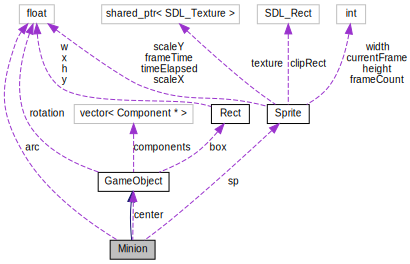
\includegraphics[width=350pt]{classMinion__coll__graph}
\end{center}
\end{figure}
\subsection*{Métodos Públicos}
\begin{DoxyCompactItemize}
\item 
\hyperlink{classMinion_a40ae7be8aa16177d2453b6102388c0f2}{Minion} (\hyperlink{classGameObject}{Game\+Object} $\ast$minion\+Center, float arc\+Offset=0)
\item 
void \hyperlink{classMinion_a5a9a53136ca0ee5fd5766410ff9acaa6}{Update} (float dt)
\item 
void \hyperlink{classMinion_af62874486a43cd5d4ecc84d9361c58dc}{Render} (void)
\item 
bool \hyperlink{classMinion_a9743cf683c7860011c56523818cc14cb}{Is\+Dead} (void)
\item 
void \hyperlink{classMinion_a43716aa99bb6afef3c40590a259de6b3}{Shoot} (\hyperlink{classVec2}{Vec2} pos)
\item 
void \hyperlink{classMinion_a908a2d009bad951df8bfd40067074059}{Notify\+Collision} (\hyperlink{classGameObject}{Game\+Object} \&other)
\item 
bool \hyperlink{classMinion_a27b0afce19e3ab3e4c76615d5902207e}{Is} (string type)
\end{DoxyCompactItemize}
\subsection*{Atributos Privados}
\begin{DoxyCompactItemize}
\item 
\hyperlink{classGameObject}{Game\+Object} $\ast$ \hyperlink{classMinion_aec145adaab9c6ecfb35b7ec1624ab111}{center}
\item 
\hyperlink{classSprite}{Sprite} \hyperlink{classMinion_a691b1b9f494fcd1f0b8c04c28ab3fa36}{sp}
\item 
float \hyperlink{classMinion_a32bbf5d39ca2f909c19c0ff9141336be}{arc}
\end{DoxyCompactItemize}
\subsection*{Additional Inherited Members}


\subsection{Construtores \& Destrutores}
\hypertarget{classMinion_a40ae7be8aa16177d2453b6102388c0f2}{\index{Minion@{Minion}!Minion@{Minion}}
\index{Minion@{Minion}!Minion@{Minion}}
\subsubsection[{Minion}]{\setlength{\rightskip}{0pt plus 5cm}Minion\+::\+Minion (
\begin{DoxyParamCaption}
\item[{{\bf Game\+Object} $\ast$}]{minion\+Center, }
\item[{float}]{arc\+Offset = {\ttfamily 0}}
\end{DoxyParamCaption}
)}}\label{classMinion_a40ae7be8aa16177d2453b6102388c0f2}


\subsection{Métodos}
\hypertarget{classMinion_a27b0afce19e3ab3e4c76615d5902207e}{\index{Minion@{Minion}!Is@{Is}}
\index{Is@{Is}!Minion@{Minion}}
\subsubsection[{Is}]{\setlength{\rightskip}{0pt plus 5cm}bool Minion\+::\+Is (
\begin{DoxyParamCaption}
\item[{string}]{type}
\end{DoxyParamCaption}
)\hspace{0.3cm}{\ttfamily [virtual]}}}\label{classMinion_a27b0afce19e3ab3e4c76615d5902207e}


Implementa \hyperlink{classGameObject_a3ddba599a800d774463c7082b7ef4801}{Game\+Object}.

\hypertarget{classMinion_a9743cf683c7860011c56523818cc14cb}{\index{Minion@{Minion}!Is\+Dead@{Is\+Dead}}
\index{Is\+Dead@{Is\+Dead}!Minion@{Minion}}
\subsubsection[{Is\+Dead}]{\setlength{\rightskip}{0pt plus 5cm}bool Minion\+::\+Is\+Dead (
\begin{DoxyParamCaption}
\item[{void}]{}
\end{DoxyParamCaption}
)\hspace{0.3cm}{\ttfamily [virtual]}}}\label{classMinion_a9743cf683c7860011c56523818cc14cb}


Implementa \hyperlink{classGameObject_a076afa2ea9190c49046f86a0946b4543}{Game\+Object}.

\hypertarget{classMinion_a908a2d009bad951df8bfd40067074059}{\index{Minion@{Minion}!Notify\+Collision@{Notify\+Collision}}
\index{Notify\+Collision@{Notify\+Collision}!Minion@{Minion}}
\subsubsection[{Notify\+Collision}]{\setlength{\rightskip}{0pt plus 5cm}void Minion\+::\+Notify\+Collision (
\begin{DoxyParamCaption}
\item[{{\bf Game\+Object} \&}]{other}
\end{DoxyParamCaption}
)\hspace{0.3cm}{\ttfamily [virtual]}}}\label{classMinion_a908a2d009bad951df8bfd40067074059}


Implementa \hyperlink{classGameObject_aa627e6c2913983fc5f108c1c4d303eb8}{Game\+Object}.

\hypertarget{classMinion_af62874486a43cd5d4ecc84d9361c58dc}{\index{Minion@{Minion}!Render@{Render}}
\index{Render@{Render}!Minion@{Minion}}
\subsubsection[{Render}]{\setlength{\rightskip}{0pt plus 5cm}void Minion\+::\+Render (
\begin{DoxyParamCaption}
\item[{void}]{}
\end{DoxyParamCaption}
)\hspace{0.3cm}{\ttfamily [virtual]}}}\label{classMinion_af62874486a43cd5d4ecc84d9361c58dc}


Implementa \hyperlink{classGameObject_a976b9c0d72212389603802f95b3f3424}{Game\+Object}.

\hypertarget{classMinion_a43716aa99bb6afef3c40590a259de6b3}{\index{Minion@{Minion}!Shoot@{Shoot}}
\index{Shoot@{Shoot}!Minion@{Minion}}
\subsubsection[{Shoot}]{\setlength{\rightskip}{0pt plus 5cm}void Minion\+::\+Shoot (
\begin{DoxyParamCaption}
\item[{{\bf Vec2}}]{pos}
\end{DoxyParamCaption}
)}}\label{classMinion_a43716aa99bb6afef3c40590a259de6b3}
\hypertarget{classMinion_a5a9a53136ca0ee5fd5766410ff9acaa6}{\index{Minion@{Minion}!Update@{Update}}
\index{Update@{Update}!Minion@{Minion}}
\subsubsection[{Update}]{\setlength{\rightskip}{0pt plus 5cm}void Minion\+::\+Update (
\begin{DoxyParamCaption}
\item[{float}]{dt}
\end{DoxyParamCaption}
)\hspace{0.3cm}{\ttfamily [virtual]}}}\label{classMinion_a5a9a53136ca0ee5fd5766410ff9acaa6}


Implementa \hyperlink{classGameObject_a93ed63df640deb516a020530e7f8e045}{Game\+Object}.



\subsection{Atributos}
\hypertarget{classMinion_a32bbf5d39ca2f909c19c0ff9141336be}{\index{Minion@{Minion}!arc@{arc}}
\index{arc@{arc}!Minion@{Minion}}
\subsubsection[{arc}]{\setlength{\rightskip}{0pt plus 5cm}float Minion\+::arc\hspace{0.3cm}{\ttfamily [private]}}}\label{classMinion_a32bbf5d39ca2f909c19c0ff9141336be}
\hypertarget{classMinion_aec145adaab9c6ecfb35b7ec1624ab111}{\index{Minion@{Minion}!center@{center}}
\index{center@{center}!Minion@{Minion}}
\subsubsection[{center}]{\setlength{\rightskip}{0pt plus 5cm}{\bf Game\+Object}$\ast$ Minion\+::center\hspace{0.3cm}{\ttfamily [private]}}}\label{classMinion_aec145adaab9c6ecfb35b7ec1624ab111}
\hypertarget{classMinion_a691b1b9f494fcd1f0b8c04c28ab3fa36}{\index{Minion@{Minion}!sp@{sp}}
\index{sp@{sp}!Minion@{Minion}}
\subsubsection[{sp}]{\setlength{\rightskip}{0pt plus 5cm}{\bf Sprite} Minion\+::sp\hspace{0.3cm}{\ttfamily [private]}}}\label{classMinion_a691b1b9f494fcd1f0b8c04c28ab3fa36}


A documentação para esta classe foi gerada a partir dos seguintes arquivos\+:\begin{DoxyCompactItemize}
\item 
Game/include/\hyperlink{Minion_8h}{Minion.\+h}\item 
Game/src/\hyperlink{Minion_8cpp}{Minion.\+cpp}\end{DoxyCompactItemize}

\hypertarget{classMusic}{\section{Referência da Classe Music}
\label{classMusic}\index{Music@{Music}}
}


{\ttfamily \#include $<$Music.\+h$>$}



Diagrama de colaboração para Music\+:\nopagebreak
\begin{figure}[H]
\begin{center}
\leavevmode
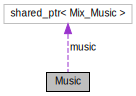
\includegraphics[width=208pt]{classMusic__coll__graph}
\end{center}
\end{figure}
\subsection*{Métodos Públicos}
\begin{DoxyCompactItemize}
\item 
\hyperlink{classMusic_ab5143f67c021bc77894c8e91de2b916b}{Music} ()
\item 
\hyperlink{classMusic_a769113513e796dd408b4deb7e758074d}{Music} (string file)
\item 
void \hyperlink{classMusic_a0b0eeff26dedfaab92bd127bce028b9a}{Play} (int times)
\item 
void \hyperlink{classMusic_a76ee0c7654f3048045e1f1b7fde334c3}{Stop} (void)
\item 
void \hyperlink{classMusic_ae13bd9609c4bb402a04f53ec07890aa3}{Open} (string file)
\item 
bool \hyperlink{classMusic_a7dd0d191e358d600f0ea8a1db75f833d}{Is\+Open} (void) const 
\end{DoxyCompactItemize}
\subsection*{Atributos Privados}
\begin{DoxyCompactItemize}
\item 
std\+::shared\+\_\+ptr$<$ Mix\+\_\+\+Music $>$ \hyperlink{classMusic_a6cddb36711f395497d2daf3e3c955912}{music}
\end{DoxyCompactItemize}


\subsection{Construtores \& Destrutores}
\hypertarget{classMusic_ab5143f67c021bc77894c8e91de2b916b}{\index{Music@{Music}!Music@{Music}}
\index{Music@{Music}!Music@{Music}}
\subsubsection[{Music}]{\setlength{\rightskip}{0pt plus 5cm}Music\+::\+Music (
\begin{DoxyParamCaption}
{}
\end{DoxyParamCaption}
)}}\label{classMusic_ab5143f67c021bc77894c8e91de2b916b}
\hypertarget{classMusic_a769113513e796dd408b4deb7e758074d}{\index{Music@{Music}!Music@{Music}}
\index{Music@{Music}!Music@{Music}}
\subsubsection[{Music}]{\setlength{\rightskip}{0pt plus 5cm}Music\+::\+Music (
\begin{DoxyParamCaption}
\item[{string}]{file}
\end{DoxyParamCaption}
)}}\label{classMusic_a769113513e796dd408b4deb7e758074d}


\subsection{Métodos}
\hypertarget{classMusic_a7dd0d191e358d600f0ea8a1db75f833d}{\index{Music@{Music}!Is\+Open@{Is\+Open}}
\index{Is\+Open@{Is\+Open}!Music@{Music}}
\subsubsection[{Is\+Open}]{\setlength{\rightskip}{0pt plus 5cm}bool Music\+::\+Is\+Open (
\begin{DoxyParamCaption}
\item[{void}]{}
\end{DoxyParamCaption}
) const}}\label{classMusic_a7dd0d191e358d600f0ea8a1db75f833d}
\hypertarget{classMusic_ae13bd9609c4bb402a04f53ec07890aa3}{\index{Music@{Music}!Open@{Open}}
\index{Open@{Open}!Music@{Music}}
\subsubsection[{Open}]{\setlength{\rightskip}{0pt plus 5cm}void Music\+::\+Open (
\begin{DoxyParamCaption}
\item[{string}]{file}
\end{DoxyParamCaption}
)}}\label{classMusic_ae13bd9609c4bb402a04f53ec07890aa3}
\hypertarget{classMusic_a0b0eeff26dedfaab92bd127bce028b9a}{\index{Music@{Music}!Play@{Play}}
\index{Play@{Play}!Music@{Music}}
\subsubsection[{Play}]{\setlength{\rightskip}{0pt plus 5cm}void Music\+::\+Play (
\begin{DoxyParamCaption}
\item[{int}]{times}
\end{DoxyParamCaption}
)}}\label{classMusic_a0b0eeff26dedfaab92bd127bce028b9a}
\hypertarget{classMusic_a76ee0c7654f3048045e1f1b7fde334c3}{\index{Music@{Music}!Stop@{Stop}}
\index{Stop@{Stop}!Music@{Music}}
\subsubsection[{Stop}]{\setlength{\rightskip}{0pt plus 5cm}void Music\+::\+Stop (
\begin{DoxyParamCaption}
\item[{void}]{}
\end{DoxyParamCaption}
)}}\label{classMusic_a76ee0c7654f3048045e1f1b7fde334c3}


\subsection{Atributos}
\hypertarget{classMusic_a6cddb36711f395497d2daf3e3c955912}{\index{Music@{Music}!music@{music}}
\index{music@{music}!Music@{Music}}
\subsubsection[{music}]{\setlength{\rightskip}{0pt plus 5cm}std\+::shared\+\_\+ptr$<$Mix\+\_\+\+Music$>$ Music\+::music\hspace{0.3cm}{\ttfamily [private]}}}\label{classMusic_a6cddb36711f395497d2daf3e3c955912}


A documentação para esta classe foi gerada a partir dos seguintes arquivos\+:\begin{DoxyCompactItemize}
\item 
Engine/include/\hyperlink{Music_8h}{Music.\+h}\item 
Engine/src/\hyperlink{Music_8cpp}{Music.\+cpp}\end{DoxyCompactItemize}

\hypertarget{classPenguins}{\section{Referência da Classe Penguins}
\label{classPenguins}\index{Penguins@{Penguins}}
}


{\ttfamily \#include $<$Penguins.\+h$>$}



Diagrama de Hierarquia para Penguins\+:\nopagebreak
\begin{figure}[H]
\begin{center}
\leavevmode
\includegraphics[width=151pt]{classPenguins__inherit__graph}
\end{center}
\end{figure}


Diagrama de colaboração para Penguins\+:
\nopagebreak
\begin{figure}[H]
\begin{center}
\leavevmode
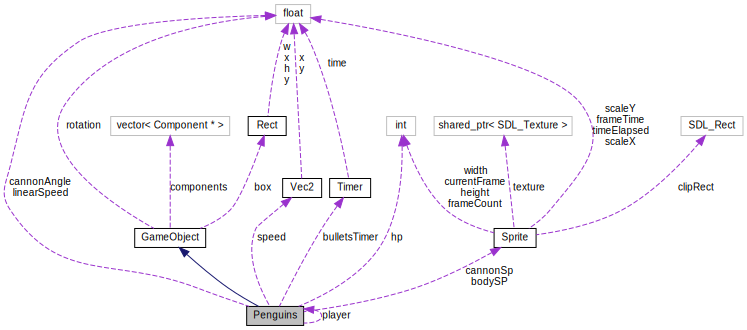
\includegraphics[width=350pt]{classPenguins__coll__graph}
\end{center}
\end{figure}
\subsection*{Métodos Públicos}
\begin{DoxyCompactItemize}
\item 
\hyperlink{classPenguins_ac87a9d6a759c4870594a167e005aae9e}{Penguins} (float x, float y)
\item 
\hyperlink{classPenguins_a685a9c6e30a94476d4dadc8bcf845211}{$\sim$\+Penguins} ()
\item 
void \hyperlink{classPenguins_a63b378e640cd3a76cbe6afaf0c6578d7}{Update} (float dt)
\item 
void \hyperlink{classPenguins_a5af1c983add97265c7491d17d2dc019e}{Render} (void)
\item 
bool \hyperlink{classPenguins_ab76c07904df3da2d768f08eb3da3d1e0}{Is\+Dead} (void)
\item 
void \hyperlink{classPenguins_a20b86d9efb0eee5169658bc57f6fc61b}{Shoot} (void)
\item 
void \hyperlink{classPenguins_aba0e8bc9309f056d196cd0fd267fbe78}{Notify\+Collision} (\hyperlink{classGameObject}{Game\+Object} \&other)
\item 
bool \hyperlink{classPenguins_a73a0c4f96de975d6219b4d6016fac29e}{Is} (string type)
\end{DoxyCompactItemize}
\subsection*{Atributos Estáticos Públicos}
\begin{DoxyCompactItemize}
\item 
static \hyperlink{classPenguins}{Penguins} $\ast$ \hyperlink{classPenguins_a7d530cec6ba98b902c6120a90d574c0f}{player} = nullptr
\end{DoxyCompactItemize}
\subsection*{Métodos Privados}
\begin{DoxyCompactItemize}
\item 
void \hyperlink{classPenguins_a5f1be8c9d5de19d15b3bbcf12e224956}{Check\+Map\+Limits} (void)
\end{DoxyCompactItemize}
\subsection*{Atributos Privados}
\begin{DoxyCompactItemize}
\item 
\hyperlink{classSprite}{Sprite} \hyperlink{classPenguins_a8073784e6c016a2bd44a306cdc0d0027}{body\+S\+P}
\item 
\hyperlink{classSprite}{Sprite} \hyperlink{classPenguins_a7e2ee1ab898ff561288c79882862e6c0}{cannon\+Sp}
\item 
\hyperlink{classVec2}{Vec2} \hyperlink{classPenguins_a7465442ffa391ddbe59486cf8475abcb}{speed}
\item 
float \hyperlink{classPenguins_a43abb7eaf4714f886be6c25babcdcb30}{linear\+Speed}
\item 
float \hyperlink{classPenguins_a71d44d99bbac380b45df64501523ab45}{cannon\+Angle}
\item 
int \hyperlink{classPenguins_a1d82db553867d4b84d2ce30c037c5882}{hp}
\item 
\hyperlink{classTimer}{Timer} \hyperlink{classPenguins_a8067358ae8be93b771475815b9c9d8d4}{bullets\+Timer}
\end{DoxyCompactItemize}
\subsection*{Additional Inherited Members}


\subsection{Construtores \& Destrutores}
\hypertarget{classPenguins_ac87a9d6a759c4870594a167e005aae9e}{\index{Penguins@{Penguins}!Penguins@{Penguins}}
\index{Penguins@{Penguins}!Penguins@{Penguins}}
\subsubsection[{Penguins}]{\setlength{\rightskip}{0pt plus 5cm}Penguins\+::\+Penguins (
\begin{DoxyParamCaption}
\item[{float}]{x, }
\item[{float}]{y}
\end{DoxyParamCaption}
)}}\label{classPenguins_ac87a9d6a759c4870594a167e005aae9e}
\hypertarget{classPenguins_a685a9c6e30a94476d4dadc8bcf845211}{\index{Penguins@{Penguins}!````~Penguins@{$\sim$\+Penguins}}
\index{````~Penguins@{$\sim$\+Penguins}!Penguins@{Penguins}}
\subsubsection[{$\sim$\+Penguins}]{\setlength{\rightskip}{0pt plus 5cm}Penguins\+::$\sim$\+Penguins (
\begin{DoxyParamCaption}
{}
\end{DoxyParamCaption}
)}}\label{classPenguins_a685a9c6e30a94476d4dadc8bcf845211}


\subsection{Métodos}
\hypertarget{classPenguins_a5f1be8c9d5de19d15b3bbcf12e224956}{\index{Penguins@{Penguins}!Check\+Map\+Limits@{Check\+Map\+Limits}}
\index{Check\+Map\+Limits@{Check\+Map\+Limits}!Penguins@{Penguins}}
\subsubsection[{Check\+Map\+Limits}]{\setlength{\rightskip}{0pt plus 5cm}void Penguins\+::\+Check\+Map\+Limits (
\begin{DoxyParamCaption}
\item[{void}]{}
\end{DoxyParamCaption}
)\hspace{0.3cm}{\ttfamily [private]}}}\label{classPenguins_a5f1be8c9d5de19d15b3bbcf12e224956}
\hypertarget{classPenguins_a73a0c4f96de975d6219b4d6016fac29e}{\index{Penguins@{Penguins}!Is@{Is}}
\index{Is@{Is}!Penguins@{Penguins}}
\subsubsection[{Is}]{\setlength{\rightskip}{0pt plus 5cm}bool Penguins\+::\+Is (
\begin{DoxyParamCaption}
\item[{string}]{type}
\end{DoxyParamCaption}
)\hspace{0.3cm}{\ttfamily [virtual]}}}\label{classPenguins_a73a0c4f96de975d6219b4d6016fac29e}


Implementa \hyperlink{classGameObject_a3ddba599a800d774463c7082b7ef4801}{Game\+Object}.

\hypertarget{classPenguins_ab76c07904df3da2d768f08eb3da3d1e0}{\index{Penguins@{Penguins}!Is\+Dead@{Is\+Dead}}
\index{Is\+Dead@{Is\+Dead}!Penguins@{Penguins}}
\subsubsection[{Is\+Dead}]{\setlength{\rightskip}{0pt plus 5cm}bool Penguins\+::\+Is\+Dead (
\begin{DoxyParamCaption}
\item[{void}]{}
\end{DoxyParamCaption}
)\hspace{0.3cm}{\ttfamily [virtual]}}}\label{classPenguins_ab76c07904df3da2d768f08eb3da3d1e0}


Implementa \hyperlink{classGameObject_a076afa2ea9190c49046f86a0946b4543}{Game\+Object}.

\hypertarget{classPenguins_aba0e8bc9309f056d196cd0fd267fbe78}{\index{Penguins@{Penguins}!Notify\+Collision@{Notify\+Collision}}
\index{Notify\+Collision@{Notify\+Collision}!Penguins@{Penguins}}
\subsubsection[{Notify\+Collision}]{\setlength{\rightskip}{0pt plus 5cm}void Penguins\+::\+Notify\+Collision (
\begin{DoxyParamCaption}
\item[{{\bf Game\+Object} \&}]{other}
\end{DoxyParamCaption}
)\hspace{0.3cm}{\ttfamily [virtual]}}}\label{classPenguins_aba0e8bc9309f056d196cd0fd267fbe78}


Implementa \hyperlink{classGameObject_aa627e6c2913983fc5f108c1c4d303eb8}{Game\+Object}.

\hypertarget{classPenguins_a5af1c983add97265c7491d17d2dc019e}{\index{Penguins@{Penguins}!Render@{Render}}
\index{Render@{Render}!Penguins@{Penguins}}
\subsubsection[{Render}]{\setlength{\rightskip}{0pt plus 5cm}void Penguins\+::\+Render (
\begin{DoxyParamCaption}
\item[{void}]{}
\end{DoxyParamCaption}
)\hspace{0.3cm}{\ttfamily [virtual]}}}\label{classPenguins_a5af1c983add97265c7491d17d2dc019e}


Implementa \hyperlink{classGameObject_a976b9c0d72212389603802f95b3f3424}{Game\+Object}.

\hypertarget{classPenguins_a20b86d9efb0eee5169658bc57f6fc61b}{\index{Penguins@{Penguins}!Shoot@{Shoot}}
\index{Shoot@{Shoot}!Penguins@{Penguins}}
\subsubsection[{Shoot}]{\setlength{\rightskip}{0pt plus 5cm}void Penguins\+::\+Shoot (
\begin{DoxyParamCaption}
\item[{void}]{}
\end{DoxyParamCaption}
)}}\label{classPenguins_a20b86d9efb0eee5169658bc57f6fc61b}
\hypertarget{classPenguins_a63b378e640cd3a76cbe6afaf0c6578d7}{\index{Penguins@{Penguins}!Update@{Update}}
\index{Update@{Update}!Penguins@{Penguins}}
\subsubsection[{Update}]{\setlength{\rightskip}{0pt plus 5cm}void Penguins\+::\+Update (
\begin{DoxyParamCaption}
\item[{float}]{dt}
\end{DoxyParamCaption}
)\hspace{0.3cm}{\ttfamily [virtual]}}}\label{classPenguins_a63b378e640cd3a76cbe6afaf0c6578d7}


Implementa \hyperlink{classGameObject_a93ed63df640deb516a020530e7f8e045}{Game\+Object}.



\subsection{Atributos}
\hypertarget{classPenguins_a8073784e6c016a2bd44a306cdc0d0027}{\index{Penguins@{Penguins}!body\+S\+P@{body\+S\+P}}
\index{body\+S\+P@{body\+S\+P}!Penguins@{Penguins}}
\subsubsection[{body\+S\+P}]{\setlength{\rightskip}{0pt plus 5cm}{\bf Sprite} Penguins\+::body\+S\+P\hspace{0.3cm}{\ttfamily [private]}}}\label{classPenguins_a8073784e6c016a2bd44a306cdc0d0027}
\hypertarget{classPenguins_a8067358ae8be93b771475815b9c9d8d4}{\index{Penguins@{Penguins}!bullets\+Timer@{bullets\+Timer}}
\index{bullets\+Timer@{bullets\+Timer}!Penguins@{Penguins}}
\subsubsection[{bullets\+Timer}]{\setlength{\rightskip}{0pt plus 5cm}{\bf Timer} Penguins\+::bullets\+Timer\hspace{0.3cm}{\ttfamily [private]}}}\label{classPenguins_a8067358ae8be93b771475815b9c9d8d4}
\hypertarget{classPenguins_a71d44d99bbac380b45df64501523ab45}{\index{Penguins@{Penguins}!cannon\+Angle@{cannon\+Angle}}
\index{cannon\+Angle@{cannon\+Angle}!Penguins@{Penguins}}
\subsubsection[{cannon\+Angle}]{\setlength{\rightskip}{0pt plus 5cm}float Penguins\+::cannon\+Angle\hspace{0.3cm}{\ttfamily [private]}}}\label{classPenguins_a71d44d99bbac380b45df64501523ab45}
\hypertarget{classPenguins_a7e2ee1ab898ff561288c79882862e6c0}{\index{Penguins@{Penguins}!cannon\+Sp@{cannon\+Sp}}
\index{cannon\+Sp@{cannon\+Sp}!Penguins@{Penguins}}
\subsubsection[{cannon\+Sp}]{\setlength{\rightskip}{0pt plus 5cm}{\bf Sprite} Penguins\+::cannon\+Sp\hspace{0.3cm}{\ttfamily [private]}}}\label{classPenguins_a7e2ee1ab898ff561288c79882862e6c0}
\hypertarget{classPenguins_a1d82db553867d4b84d2ce30c037c5882}{\index{Penguins@{Penguins}!hp@{hp}}
\index{hp@{hp}!Penguins@{Penguins}}
\subsubsection[{hp}]{\setlength{\rightskip}{0pt plus 5cm}int Penguins\+::hp\hspace{0.3cm}{\ttfamily [private]}}}\label{classPenguins_a1d82db553867d4b84d2ce30c037c5882}
\hypertarget{classPenguins_a43abb7eaf4714f886be6c25babcdcb30}{\index{Penguins@{Penguins}!linear\+Speed@{linear\+Speed}}
\index{linear\+Speed@{linear\+Speed}!Penguins@{Penguins}}
\subsubsection[{linear\+Speed}]{\setlength{\rightskip}{0pt plus 5cm}float Penguins\+::linear\+Speed\hspace{0.3cm}{\ttfamily [private]}}}\label{classPenguins_a43abb7eaf4714f886be6c25babcdcb30}
\hypertarget{classPenguins_a7d530cec6ba98b902c6120a90d574c0f}{\index{Penguins@{Penguins}!player@{player}}
\index{player@{player}!Penguins@{Penguins}}
\subsubsection[{player}]{\setlength{\rightskip}{0pt plus 5cm}{\bf Penguins} $\ast$ Penguins\+::player = nullptr\hspace{0.3cm}{\ttfamily [static]}}}\label{classPenguins_a7d530cec6ba98b902c6120a90d574c0f}
\hypertarget{classPenguins_a7465442ffa391ddbe59486cf8475abcb}{\index{Penguins@{Penguins}!speed@{speed}}
\index{speed@{speed}!Penguins@{Penguins}}
\subsubsection[{speed}]{\setlength{\rightskip}{0pt plus 5cm}{\bf Vec2} Penguins\+::speed\hspace{0.3cm}{\ttfamily [private]}}}\label{classPenguins_a7465442ffa391ddbe59486cf8475abcb}


A documentação para esta classe foi gerada a partir dos seguintes arquivos\+:\begin{DoxyCompactItemize}
\item 
Game/include/\hyperlink{Penguins_8h}{Penguins.\+h}\item 
Game/src/\hyperlink{Penguins_8cpp}{Penguins.\+cpp}\end{DoxyCompactItemize}

\hypertarget{classRect}{\section{Referência da Classe Rect}
\label{classRect}\index{Rect@{Rect}}
}


{\ttfamily \#include $<$Rect.\+h$>$}



Diagrama de colaboração para Rect\+:\nopagebreak
\begin{figure}[H]
\begin{center}
\leavevmode
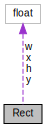
\includegraphics[width=118pt]{classRect__coll__graph}
\end{center}
\end{figure}
\subsection*{Métodos Públicos}
\begin{DoxyCompactItemize}
\item 
\hyperlink{classRect_a62fb6094640e8a5a9969382d404e9d5e}{Rect} (void)
\item 
\hyperlink{classRect_a21e3f21b1579b6aea19ea88d89c019ef}{Rect} (float \hyperlink{classRect_a29bc9b88a8c5537620f05ac7069f48cc}{x}, float \hyperlink{classRect_a4ea33d8210fa0b8b0d6ef3f7e06e6b27}{y}, float \hyperlink{classRect_a049f7ee5e7eb0475229bf3ed9b3bad44}{w}, float \hyperlink{classRect_aa10c9b8950c6b23a0b2bf0d39f2be904}{h})
\item 
\hyperlink{classRect_a9a0dccb457b32573b281e1ce7a076c8d}{operator S\+D\+L\+\_\+\+Rect} () const 
\item 
\hyperlink{classRect_a8649d07c49ee8f230b362a223fa0f5e9}{operator Vec2} () const 
\item 
\hyperlink{classRect}{Rect} \hyperlink{classRect_af3213bdcfa1920ab6b5fed108ac5c374}{operator+} (\hyperlink{classVec2}{Vec2} const \&a) const 
\item 
\hyperlink{classRect}{Rect} \hyperlink{classRect_af033df220edef5de3488e18c163b2b39}{operator-\/} (\hyperlink{classVec2}{Vec2} const \&a) const 
\item 
\hyperlink{classRect}{Rect} \hyperlink{classRect_aca144c3e9d36600106932e22a5659513}{operator=} (\hyperlink{classVec2}{Vec2} const \&a)
\item 
\hyperlink{classRect}{Rect} \hyperlink{classRect_a42a400642b9e5d2895a6c432ff11a168}{operator$\ast$} (float const zoom) const 
\item 
\hyperlink{classVec2}{Vec2} \hyperlink{classRect_ac42ead7988bf077364ce61231980bff2}{Center} (void) const 
\item 
void \hyperlink{classRect_a5751026840c842f72e1f79cb82d9554c}{Set\+Width\+And\+Height} (\hyperlink{classVec2}{Vec2} const \&vec)
\end{DoxyCompactItemize}
\subsection*{Atributos Públicos}
\begin{DoxyCompactItemize}
\item 
float \hyperlink{classRect_a29bc9b88a8c5537620f05ac7069f48cc}{x}
\item 
float \hyperlink{classRect_a4ea33d8210fa0b8b0d6ef3f7e06e6b27}{y}
\item 
float \hyperlink{classRect_a049f7ee5e7eb0475229bf3ed9b3bad44}{w}
\item 
float \hyperlink{classRect_aa10c9b8950c6b23a0b2bf0d39f2be904}{h}
\end{DoxyCompactItemize}


\subsection{Construtores \& Destrutores}
\hypertarget{classRect_a62fb6094640e8a5a9969382d404e9d5e}{\index{Rect@{Rect}!Rect@{Rect}}
\index{Rect@{Rect}!Rect@{Rect}}
\subsubsection[{Rect}]{\setlength{\rightskip}{0pt plus 5cm}Rect\+::\+Rect (
\begin{DoxyParamCaption}
\item[{void}]{}
\end{DoxyParamCaption}
)}}\label{classRect_a62fb6094640e8a5a9969382d404e9d5e}
\hypertarget{classRect_a21e3f21b1579b6aea19ea88d89c019ef}{\index{Rect@{Rect}!Rect@{Rect}}
\index{Rect@{Rect}!Rect@{Rect}}
\subsubsection[{Rect}]{\setlength{\rightskip}{0pt plus 5cm}Rect\+::\+Rect (
\begin{DoxyParamCaption}
\item[{float}]{x, }
\item[{float}]{y, }
\item[{float}]{w, }
\item[{float}]{h}
\end{DoxyParamCaption}
)}}\label{classRect_a21e3f21b1579b6aea19ea88d89c019ef}


\subsection{Métodos}
\hypertarget{classRect_ac42ead7988bf077364ce61231980bff2}{\index{Rect@{Rect}!Center@{Center}}
\index{Center@{Center}!Rect@{Rect}}
\subsubsection[{Center}]{\setlength{\rightskip}{0pt plus 5cm}{\bf Vec2} Rect\+::\+Center (
\begin{DoxyParamCaption}
\item[{void}]{}
\end{DoxyParamCaption}
) const}}\label{classRect_ac42ead7988bf077364ce61231980bff2}
\hypertarget{classRect_a9a0dccb457b32573b281e1ce7a076c8d}{\index{Rect@{Rect}!operator S\+D\+L\+\_\+\+Rect@{operator S\+D\+L\+\_\+\+Rect}}
\index{operator S\+D\+L\+\_\+\+Rect@{operator S\+D\+L\+\_\+\+Rect}!Rect@{Rect}}
\subsubsection[{operator S\+D\+L\+\_\+\+Rect}]{\setlength{\rightskip}{0pt plus 5cm}Rect\+::operator S\+D\+L\+\_\+\+Rect (
\begin{DoxyParamCaption}
{}
\end{DoxyParamCaption}
) const}}\label{classRect_a9a0dccb457b32573b281e1ce7a076c8d}
\hypertarget{classRect_a8649d07c49ee8f230b362a223fa0f5e9}{\index{Rect@{Rect}!operator Vec2@{operator Vec2}}
\index{operator Vec2@{operator Vec2}!Rect@{Rect}}
\subsubsection[{operator Vec2}]{\setlength{\rightskip}{0pt plus 5cm}Rect\+::operator {\bf Vec2} (
\begin{DoxyParamCaption}
{}
\end{DoxyParamCaption}
) const}}\label{classRect_a8649d07c49ee8f230b362a223fa0f5e9}
\hypertarget{classRect_a42a400642b9e5d2895a6c432ff11a168}{\index{Rect@{Rect}!operator$\ast$@{operator$\ast$}}
\index{operator$\ast$@{operator$\ast$}!Rect@{Rect}}
\subsubsection[{operator$\ast$}]{\setlength{\rightskip}{0pt plus 5cm}{\bf Rect} Rect\+::operator$\ast$ (
\begin{DoxyParamCaption}
\item[{float const}]{zoom}
\end{DoxyParamCaption}
) const}}\label{classRect_a42a400642b9e5d2895a6c432ff11a168}
\hypertarget{classRect_af3213bdcfa1920ab6b5fed108ac5c374}{\index{Rect@{Rect}!operator+@{operator+}}
\index{operator+@{operator+}!Rect@{Rect}}
\subsubsection[{operator+}]{\setlength{\rightskip}{0pt plus 5cm}{\bf Rect} Rect\+::operator+ (
\begin{DoxyParamCaption}
\item[{{\bf Vec2} const \&}]{a}
\end{DoxyParamCaption}
) const}}\label{classRect_af3213bdcfa1920ab6b5fed108ac5c374}
\hypertarget{classRect_af033df220edef5de3488e18c163b2b39}{\index{Rect@{Rect}!operator-\/@{operator-\/}}
\index{operator-\/@{operator-\/}!Rect@{Rect}}
\subsubsection[{operator-\/}]{\setlength{\rightskip}{0pt plus 5cm}{\bf Rect} Rect\+::operator-\/ (
\begin{DoxyParamCaption}
\item[{{\bf Vec2} const \&}]{a}
\end{DoxyParamCaption}
) const}}\label{classRect_af033df220edef5de3488e18c163b2b39}
\hypertarget{classRect_aca144c3e9d36600106932e22a5659513}{\index{Rect@{Rect}!operator=@{operator=}}
\index{operator=@{operator=}!Rect@{Rect}}
\subsubsection[{operator=}]{\setlength{\rightskip}{0pt plus 5cm}{\bf Rect} Rect\+::operator= (
\begin{DoxyParamCaption}
\item[{{\bf Vec2} const \&}]{a}
\end{DoxyParamCaption}
)}}\label{classRect_aca144c3e9d36600106932e22a5659513}
\hypertarget{classRect_a5751026840c842f72e1f79cb82d9554c}{\index{Rect@{Rect}!Set\+Width\+And\+Height@{Set\+Width\+And\+Height}}
\index{Set\+Width\+And\+Height@{Set\+Width\+And\+Height}!Rect@{Rect}}
\subsubsection[{Set\+Width\+And\+Height}]{\setlength{\rightskip}{0pt plus 5cm}void Rect\+::\+Set\+Width\+And\+Height (
\begin{DoxyParamCaption}
\item[{{\bf Vec2} const \&}]{vec}
\end{DoxyParamCaption}
)}}\label{classRect_a5751026840c842f72e1f79cb82d9554c}


\subsection{Atributos}
\hypertarget{classRect_aa10c9b8950c6b23a0b2bf0d39f2be904}{\index{Rect@{Rect}!h@{h}}
\index{h@{h}!Rect@{Rect}}
\subsubsection[{h}]{\setlength{\rightskip}{0pt plus 5cm}float Rect\+::h}}\label{classRect_aa10c9b8950c6b23a0b2bf0d39f2be904}
\hypertarget{classRect_a049f7ee5e7eb0475229bf3ed9b3bad44}{\index{Rect@{Rect}!w@{w}}
\index{w@{w}!Rect@{Rect}}
\subsubsection[{w}]{\setlength{\rightskip}{0pt plus 5cm}float Rect\+::w}}\label{classRect_a049f7ee5e7eb0475229bf3ed9b3bad44}
\hypertarget{classRect_a29bc9b88a8c5537620f05ac7069f48cc}{\index{Rect@{Rect}!x@{x}}
\index{x@{x}!Rect@{Rect}}
\subsubsection[{x}]{\setlength{\rightskip}{0pt plus 5cm}float Rect\+::x}}\label{classRect_a29bc9b88a8c5537620f05ac7069f48cc}
\hypertarget{classRect_a4ea33d8210fa0b8b0d6ef3f7e06e6b27}{\index{Rect@{Rect}!y@{y}}
\index{y@{y}!Rect@{Rect}}
\subsubsection[{y}]{\setlength{\rightskip}{0pt plus 5cm}float Rect\+::y}}\label{classRect_a4ea33d8210fa0b8b0d6ef3f7e06e6b27}


A documentação para esta classe foi gerada a partir dos seguintes arquivos\+:\begin{DoxyCompactItemize}
\item 
Engine/include/\hyperlink{Rect_8h}{Rect.\+h}\item 
Engine/src/\hyperlink{Rect_8cpp}{Rect.\+cpp}\end{DoxyCompactItemize}

\hypertarget{classResources}{\section{Referência da Classe Resources}
\label{classResources}\index{Resources@{Resources}}
}


{\ttfamily \#include $<$Resources.\+h$>$}



Diagrama de colaboração para Resources\+:\nopagebreak
\begin{figure}[H]
\begin{center}
\leavevmode
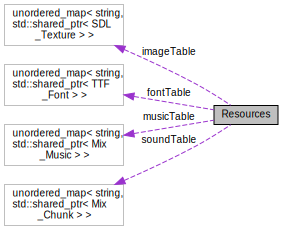
\includegraphics[width=350pt]{classResources__coll__graph}
\end{center}
\end{figure}
\subsection*{Métodos Públicos Estáticos}
\begin{DoxyCompactItemize}
\item 
static std\+::shared\+\_\+ptr\\*
$<$ S\+D\+L\+\_\+\+Texture $>$ \hyperlink{classResources_a557aa346c974a8bce80017dbabd653d9}{Get\+Image} (string file)
\item 
static std\+::shared\+\_\+ptr$<$ Mix\+\_\+\+Music $>$ \hyperlink{classResources_a9ed99125bc4d75514e1175fab6f9badf}{Get\+Music} (string file)
\item 
static std\+::shared\+\_\+ptr$<$ Mix\+\_\+\+Chunk $>$ \hyperlink{classResources_ae6e4e0202dec020da8f6654f685e8b98}{Get\+Sound} (string file)
\item 
static std\+::shared\+\_\+ptr$<$ T\+T\+F\+\_\+\+Font $>$ \hyperlink{classResources_a661a92ea82fb73e31092059d6fc383c3}{Get\+Font} (string file, int font\+Size)
\item 
static void \hyperlink{classResources_a6a704f9988d9189d2d028ab5dcc64496}{Clear\+Resources} (void)
\end{DoxyCompactItemize}
\subsection*{Métodos Privados}
\begin{DoxyCompactItemize}
\item 
\hyperlink{classResources_ab09435991b8c485f92e0aa1fd00828b9}{Resources} ()
\end{DoxyCompactItemize}
\subsection*{Métodos Privados Estáticos}
\begin{DoxyCompactItemize}
\item 
static void \hyperlink{classResources_a6f83b82e64c61691b60e6aed70b6ab68}{Clear\+Images} (void)
\item 
static void \hyperlink{classResources_a37aa5ada5adf925b8862f65d207244d1}{Clear\+Music} (void)
\item 
static void \hyperlink{classResources_a07885930484a8dd953c2e144ac8be6c5}{Clear\+Sound} (void)
\item 
static void \hyperlink{classResources_abfa5ce49b74cb81a0f3c7a47d94e0eda}{Clear\+Fonts} (void)
\end{DoxyCompactItemize}
\subsection*{Atributos Privados Estáticos}
\begin{DoxyCompactItemize}
\item 
static std\+::unordered\+\_\+map\\*
$<$ string, std\+::shared\+\_\+ptr\\*
$<$ S\+D\+L\+\_\+\+Texture $>$ $>$ \hyperlink{classResources_abb18128c6fd91ee3afe41c1947c42b02}{image\+Table}
\item 
static std\+::unordered\+\_\+map\\*
$<$ string, std\+::shared\+\_\+ptr\\*
$<$ Mix\+\_\+\+Music $>$ $>$ \hyperlink{classResources_a6fa55a3d59924e7fbbcf734e01cfaa46}{music\+Table}
\item 
static std\+::unordered\+\_\+map\\*
$<$ string, std\+::shared\+\_\+ptr\\*
$<$ Mix\+\_\+\+Chunk $>$ $>$ \hyperlink{classResources_abbd116a3bc870ba6578a89b4aa08908c}{sound\+Table}
\item 
static std\+::unordered\+\_\+map\\*
$<$ string, std\+::shared\+\_\+ptr\\*
$<$ T\+T\+F\+\_\+\+Font $>$ $>$ \hyperlink{classResources_ab3665e0c725cd7f4dbf65b128f87d0d5}{font\+Table}
\end{DoxyCompactItemize}


\subsection{Construtores \& Destrutores}
\hypertarget{classResources_ab09435991b8c485f92e0aa1fd00828b9}{\index{Resources@{Resources}!Resources@{Resources}}
\index{Resources@{Resources}!Resources@{Resources}}
\subsubsection[{Resources}]{\setlength{\rightskip}{0pt plus 5cm}Resources\+::\+Resources (
\begin{DoxyParamCaption}
{}
\end{DoxyParamCaption}
)\hspace{0.3cm}{\ttfamily [private]}}}\label{classResources_ab09435991b8c485f92e0aa1fd00828b9}


\subsection{Métodos}
\hypertarget{classResources_abfa5ce49b74cb81a0f3c7a47d94e0eda}{\index{Resources@{Resources}!Clear\+Fonts@{Clear\+Fonts}}
\index{Clear\+Fonts@{Clear\+Fonts}!Resources@{Resources}}
\subsubsection[{Clear\+Fonts}]{\setlength{\rightskip}{0pt plus 5cm}void Resources\+::\+Clear\+Fonts (
\begin{DoxyParamCaption}
\item[{void}]{}
\end{DoxyParamCaption}
)\hspace{0.3cm}{\ttfamily [static]}, {\ttfamily [private]}}}\label{classResources_abfa5ce49b74cb81a0f3c7a47d94e0eda}
\hypertarget{classResources_a6f83b82e64c61691b60e6aed70b6ab68}{\index{Resources@{Resources}!Clear\+Images@{Clear\+Images}}
\index{Clear\+Images@{Clear\+Images}!Resources@{Resources}}
\subsubsection[{Clear\+Images}]{\setlength{\rightskip}{0pt plus 5cm}void Resources\+::\+Clear\+Images (
\begin{DoxyParamCaption}
\item[{void}]{}
\end{DoxyParamCaption}
)\hspace{0.3cm}{\ttfamily [static]}, {\ttfamily [private]}}}\label{classResources_a6f83b82e64c61691b60e6aed70b6ab68}
\hypertarget{classResources_a37aa5ada5adf925b8862f65d207244d1}{\index{Resources@{Resources}!Clear\+Music@{Clear\+Music}}
\index{Clear\+Music@{Clear\+Music}!Resources@{Resources}}
\subsubsection[{Clear\+Music}]{\setlength{\rightskip}{0pt plus 5cm}void Resources\+::\+Clear\+Music (
\begin{DoxyParamCaption}
\item[{void}]{}
\end{DoxyParamCaption}
)\hspace{0.3cm}{\ttfamily [static]}, {\ttfamily [private]}}}\label{classResources_a37aa5ada5adf925b8862f65d207244d1}
\hypertarget{classResources_a6a704f9988d9189d2d028ab5dcc64496}{\index{Resources@{Resources}!Clear\+Resources@{Clear\+Resources}}
\index{Clear\+Resources@{Clear\+Resources}!Resources@{Resources}}
\subsubsection[{Clear\+Resources}]{\setlength{\rightskip}{0pt plus 5cm}void Resources\+::\+Clear\+Resources (
\begin{DoxyParamCaption}
\item[{void}]{}
\end{DoxyParamCaption}
)\hspace{0.3cm}{\ttfamily [static]}}}\label{classResources_a6a704f9988d9189d2d028ab5dcc64496}
\hypertarget{classResources_a07885930484a8dd953c2e144ac8be6c5}{\index{Resources@{Resources}!Clear\+Sound@{Clear\+Sound}}
\index{Clear\+Sound@{Clear\+Sound}!Resources@{Resources}}
\subsubsection[{Clear\+Sound}]{\setlength{\rightskip}{0pt plus 5cm}void Resources\+::\+Clear\+Sound (
\begin{DoxyParamCaption}
\item[{void}]{}
\end{DoxyParamCaption}
)\hspace{0.3cm}{\ttfamily [static]}, {\ttfamily [private]}}}\label{classResources_a07885930484a8dd953c2e144ac8be6c5}
\hypertarget{classResources_a661a92ea82fb73e31092059d6fc383c3}{\index{Resources@{Resources}!Get\+Font@{Get\+Font}}
\index{Get\+Font@{Get\+Font}!Resources@{Resources}}
\subsubsection[{Get\+Font}]{\setlength{\rightskip}{0pt plus 5cm}std\+::shared\+\_\+ptr$<$ T\+T\+F\+\_\+\+Font $>$ Resources\+::\+Get\+Font (
\begin{DoxyParamCaption}
\item[{string}]{file, }
\item[{int}]{font\+Size}
\end{DoxyParamCaption}
)\hspace{0.3cm}{\ttfamily [static]}}}\label{classResources_a661a92ea82fb73e31092059d6fc383c3}
\hypertarget{classResources_a557aa346c974a8bce80017dbabd653d9}{\index{Resources@{Resources}!Get\+Image@{Get\+Image}}
\index{Get\+Image@{Get\+Image}!Resources@{Resources}}
\subsubsection[{Get\+Image}]{\setlength{\rightskip}{0pt plus 5cm}std\+::shared\+\_\+ptr$<$ S\+D\+L\+\_\+\+Texture $>$ Resources\+::\+Get\+Image (
\begin{DoxyParamCaption}
\item[{string}]{file}
\end{DoxyParamCaption}
)\hspace{0.3cm}{\ttfamily [static]}}}\label{classResources_a557aa346c974a8bce80017dbabd653d9}
\hypertarget{classResources_a9ed99125bc4d75514e1175fab6f9badf}{\index{Resources@{Resources}!Get\+Music@{Get\+Music}}
\index{Get\+Music@{Get\+Music}!Resources@{Resources}}
\subsubsection[{Get\+Music}]{\setlength{\rightskip}{0pt plus 5cm}std\+::shared\+\_\+ptr$<$ Mix\+\_\+\+Music $>$ Resources\+::\+Get\+Music (
\begin{DoxyParamCaption}
\item[{string}]{file}
\end{DoxyParamCaption}
)\hspace{0.3cm}{\ttfamily [static]}}}\label{classResources_a9ed99125bc4d75514e1175fab6f9badf}
\hypertarget{classResources_ae6e4e0202dec020da8f6654f685e8b98}{\index{Resources@{Resources}!Get\+Sound@{Get\+Sound}}
\index{Get\+Sound@{Get\+Sound}!Resources@{Resources}}
\subsubsection[{Get\+Sound}]{\setlength{\rightskip}{0pt plus 5cm}std\+::shared\+\_\+ptr$<$ Mix\+\_\+\+Chunk $>$ Resources\+::\+Get\+Sound (
\begin{DoxyParamCaption}
\item[{string}]{file}
\end{DoxyParamCaption}
)\hspace{0.3cm}{\ttfamily [static]}}}\label{classResources_ae6e4e0202dec020da8f6654f685e8b98}


\subsection{Atributos}
\hypertarget{classResources_ab3665e0c725cd7f4dbf65b128f87d0d5}{\index{Resources@{Resources}!font\+Table@{font\+Table}}
\index{font\+Table@{font\+Table}!Resources@{Resources}}
\subsubsection[{font\+Table}]{\setlength{\rightskip}{0pt plus 5cm}std\+::unordered\+\_\+map$<$ string, std\+::shared\+\_\+ptr$<$ T\+T\+F\+\_\+\+Font $>$ $>$ Resources\+::font\+Table\hspace{0.3cm}{\ttfamily [static]}, {\ttfamily [private]}}}\label{classResources_ab3665e0c725cd7f4dbf65b128f87d0d5}
\hypertarget{classResources_abb18128c6fd91ee3afe41c1947c42b02}{\index{Resources@{Resources}!image\+Table@{image\+Table}}
\index{image\+Table@{image\+Table}!Resources@{Resources}}
\subsubsection[{image\+Table}]{\setlength{\rightskip}{0pt plus 5cm}std\+::unordered\+\_\+map$<$ string, std\+::shared\+\_\+ptr$<$ S\+D\+L\+\_\+\+Texture $>$ $>$ Resources\+::image\+Table\hspace{0.3cm}{\ttfamily [static]}, {\ttfamily [private]}}}\label{classResources_abb18128c6fd91ee3afe41c1947c42b02}
\hypertarget{classResources_a6fa55a3d59924e7fbbcf734e01cfaa46}{\index{Resources@{Resources}!music\+Table@{music\+Table}}
\index{music\+Table@{music\+Table}!Resources@{Resources}}
\subsubsection[{music\+Table}]{\setlength{\rightskip}{0pt plus 5cm}std\+::unordered\+\_\+map$<$ string, std\+::shared\+\_\+ptr$<$ Mix\+\_\+\+Music $>$ $>$ Resources\+::music\+Table\hspace{0.3cm}{\ttfamily [static]}, {\ttfamily [private]}}}\label{classResources_a6fa55a3d59924e7fbbcf734e01cfaa46}
\hypertarget{classResources_abbd116a3bc870ba6578a89b4aa08908c}{\index{Resources@{Resources}!sound\+Table@{sound\+Table}}
\index{sound\+Table@{sound\+Table}!Resources@{Resources}}
\subsubsection[{sound\+Table}]{\setlength{\rightskip}{0pt plus 5cm}std\+::unordered\+\_\+map$<$ string, std\+::shared\+\_\+ptr$<$ Mix\+\_\+\+Chunk $>$ $>$ Resources\+::sound\+Table\hspace{0.3cm}{\ttfamily [static]}, {\ttfamily [private]}}}\label{classResources_abbd116a3bc870ba6578a89b4aa08908c}


A documentação para esta classe foi gerada a partir dos seguintes arquivos\+:\begin{DoxyCompactItemize}
\item 
Engine/include/\hyperlink{Resources_8h}{Resources.\+h}\item 
Engine/src/\hyperlink{Resources_8cpp}{Resources.\+cpp}\end{DoxyCompactItemize}

\hypertarget{classSound}{\section{Referência da Classe Sound}
\label{classSound}\index{Sound@{Sound}}
}


{\ttfamily \#include $<$Sound.\+h$>$}



Diagrama de colaboração para Sound\+:
\nopagebreak
\begin{figure}[H]
\begin{center}
\leavevmode
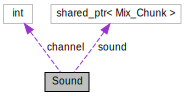
\includegraphics[width=258pt]{classSound__coll__graph}
\end{center}
\end{figure}
\subsection*{Métodos Públicos}
\begin{DoxyCompactItemize}
\item 
\hyperlink{classSound_a539c205cdf06fe2c621fd77c37bcfac9}{Sound} ()
\item 
\hyperlink{classSound_af2c277cdc12b7df1de53e5b855e4f09c}{Sound} (string file)
\item 
void \hyperlink{classSound_a2719199f31d8abfc0bd9a6814e4e169d}{Play} (int times)
\item 
void \hyperlink{classSound_ae391c15fe26a0091e601be32eef0bce5}{Stop} (void)
\item 
void \hyperlink{classSound_afa261d68708b917bf60d704238b56f87}{Open} (string file)
\item 
bool \hyperlink{classSound_a9e67e48d34d9ca3d31f0da846ada923b}{Is\+Open} (void)
\end{DoxyCompactItemize}
\subsection*{Atributos Privados}
\begin{DoxyCompactItemize}
\item 
std\+::shared\+\_\+ptr$<$ Mix\+\_\+\+Chunk $>$ \hyperlink{classSound_a44bbda770ac76c7455b60d3d63b663a7}{sound}
\item 
int \hyperlink{classSound_af3895edf5a39772f1de32cfbfff90909}{channel}
\end{DoxyCompactItemize}


\subsection{Construtores \& Destrutores}
\hypertarget{classSound_a539c205cdf06fe2c621fd77c37bcfac9}{\index{Sound@{Sound}!Sound@{Sound}}
\index{Sound@{Sound}!Sound@{Sound}}
\subsubsection[{Sound}]{\setlength{\rightskip}{0pt plus 5cm}Sound\+::\+Sound (
\begin{DoxyParamCaption}
{}
\end{DoxyParamCaption}
)}}\label{classSound_a539c205cdf06fe2c621fd77c37bcfac9}
\hypertarget{classSound_af2c277cdc12b7df1de53e5b855e4f09c}{\index{Sound@{Sound}!Sound@{Sound}}
\index{Sound@{Sound}!Sound@{Sound}}
\subsubsection[{Sound}]{\setlength{\rightskip}{0pt plus 5cm}Sound\+::\+Sound (
\begin{DoxyParamCaption}
\item[{string}]{file}
\end{DoxyParamCaption}
)}}\label{classSound_af2c277cdc12b7df1de53e5b855e4f09c}


\subsection{Métodos}
\hypertarget{classSound_a9e67e48d34d9ca3d31f0da846ada923b}{\index{Sound@{Sound}!Is\+Open@{Is\+Open}}
\index{Is\+Open@{Is\+Open}!Sound@{Sound}}
\subsubsection[{Is\+Open}]{\setlength{\rightskip}{0pt plus 5cm}bool Sound\+::\+Is\+Open (
\begin{DoxyParamCaption}
\item[{void}]{}
\end{DoxyParamCaption}
)}}\label{classSound_a9e67e48d34d9ca3d31f0da846ada923b}
\hypertarget{classSound_afa261d68708b917bf60d704238b56f87}{\index{Sound@{Sound}!Open@{Open}}
\index{Open@{Open}!Sound@{Sound}}
\subsubsection[{Open}]{\setlength{\rightskip}{0pt plus 5cm}void Sound\+::\+Open (
\begin{DoxyParamCaption}
\item[{string}]{file}
\end{DoxyParamCaption}
)}}\label{classSound_afa261d68708b917bf60d704238b56f87}
\hypertarget{classSound_a2719199f31d8abfc0bd9a6814e4e169d}{\index{Sound@{Sound}!Play@{Play}}
\index{Play@{Play}!Sound@{Sound}}
\subsubsection[{Play}]{\setlength{\rightskip}{0pt plus 5cm}void Sound\+::\+Play (
\begin{DoxyParamCaption}
\item[{int}]{times}
\end{DoxyParamCaption}
)}}\label{classSound_a2719199f31d8abfc0bd9a6814e4e169d}
\hypertarget{classSound_ae391c15fe26a0091e601be32eef0bce5}{\index{Sound@{Sound}!Stop@{Stop}}
\index{Stop@{Stop}!Sound@{Sound}}
\subsubsection[{Stop}]{\setlength{\rightskip}{0pt plus 5cm}void Sound\+::\+Stop (
\begin{DoxyParamCaption}
\item[{void}]{}
\end{DoxyParamCaption}
)}}\label{classSound_ae391c15fe26a0091e601be32eef0bce5}


\subsection{Atributos}
\hypertarget{classSound_af3895edf5a39772f1de32cfbfff90909}{\index{Sound@{Sound}!channel@{channel}}
\index{channel@{channel}!Sound@{Sound}}
\subsubsection[{channel}]{\setlength{\rightskip}{0pt plus 5cm}int Sound\+::channel\hspace{0.3cm}{\ttfamily [private]}}}\label{classSound_af3895edf5a39772f1de32cfbfff90909}
\hypertarget{classSound_a44bbda770ac76c7455b60d3d63b663a7}{\index{Sound@{Sound}!sound@{sound}}
\index{sound@{sound}!Sound@{Sound}}
\subsubsection[{sound}]{\setlength{\rightskip}{0pt plus 5cm}std\+::shared\+\_\+ptr$<$Mix\+\_\+\+Chunk$>$ Sound\+::sound\hspace{0.3cm}{\ttfamily [private]}}}\label{classSound_a44bbda770ac76c7455b60d3d63b663a7}


A documentação para esta classe foi gerada a partir dos seguintes arquivos\+:\begin{DoxyCompactItemize}
\item 
Engine/include/\hyperlink{Sound_8h}{Sound.\+h}\item 
Engine/src/\hyperlink{Sound_8cpp}{Sound.\+cpp}\end{DoxyCompactItemize}

\hypertarget{classSprite}{\section{Referência da Classe Sprite}
\label{classSprite}\index{Sprite@{Sprite}}
}


{\ttfamily \#include $<$Sprite.\+h$>$}



Diagrama de colaboração para Sprite\+:
\nopagebreak
\begin{figure}[H]
\begin{center}
\leavevmode
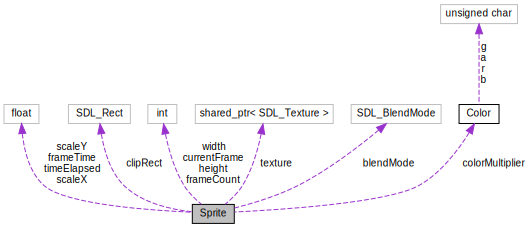
\includegraphics[width=350pt]{classSprite__coll__graph}
\end{center}
\end{figure}
\subsection*{Métodos Públicos}
\begin{DoxyCompactItemize}
\item 
\hyperlink{classSprite_abee3d268d8e467d9e23bfe0693e64144}{Sprite} (void)
\item 
\hyperlink{classSprite_a5b32e7b8aede63b8a2720ecfa670d0e3}{Sprite} (std\+::string file, float \hyperlink{classSprite_a5d41b63da1b5ee4a734ce060ab876878}{frame\+Time}=1, int \hyperlink{classSprite_a8dc8d5c9530bad6113d37fe5e53e4668}{frame\+Count}=1)
\item 
\hyperlink{classSprite_a8accab430f9d90ae5117b57d67e32b84}{$\sim$\+Sprite} ()
\item 
void \hyperlink{classSprite_a0528ea8ae39cdf864e01e2b4aaca8dca}{Open} (std\+::string file)
\item 
void \hyperlink{classSprite_a3ad46a400f83d41eaba2c2df77e0cf7c}{Set\+Clip} (int x, int y, int w, int h)
\item 
void \hyperlink{classSprite_a42afe1ad83085fb323e388f5854d9b01}{Render} (int x, int y, float angle=0, bool zoom=false) const 
\item 
int \hyperlink{classSprite_ad3d43826d2f41185964ec4a1eb492248}{Get\+Width} (void) const 
\item 
int \hyperlink{classSprite_a2a5a7c73dd94f822b0a248de3621e5eb}{Get\+Height} (void) const 
\item 
std\+::shared\+\_\+ptr$<$ S\+D\+L\+\_\+\+Texture $>$ \hyperlink{classSprite_a27148c9990eeb0efa187ec41de2d3db0}{Get\+Texture} (void) const 
\item 
bool \hyperlink{classSprite_a9f1e62573dd91cb03dbad7aa54807b8c}{Is\+Open} (void) const 
\item 
void \hyperlink{classSprite_a1f5ac7fbd3e6efeca11cedb6b822df43}{Update} (float dt)
\item 
void \hyperlink{classSprite_a351dd54dac6cadbbdec48f9e1d8a36c0}{Set\+Frame} (int frame)
\item 
void \hyperlink{classSprite_adf5254476a027570a0112cf48979f3a5}{Set\+Frame\+Count} (int \hyperlink{classSprite_a8dc8d5c9530bad6113d37fe5e53e4668}{frame\+Count})
\item 
void \hyperlink{classSprite_a8ebb93cd7485a51ccc635819ded6349b}{Set\+Frame\+Time} (float \hyperlink{classSprite_a5d41b63da1b5ee4a734ce060ab876878}{frame\+Time})
\item 
void \hyperlink{classSprite_aad7bb29fc017ac2197dffec177c17e15}{Set\+Scale\+X} (float scale)
\item 
void \hyperlink{classSprite_a2853ee7687dc906b9be791d197a1b1b6}{Set\+Scale\+Y} (float scale)
\item 
void \hyperlink{classSprite_a54d18a18383575b04f397f5bec3113d0}{Set\+Scale} (float scale)
\item 
void \hyperlink{classSprite_a42b3a6ed82560c5b97085cc127984cf4}{Scale\+X} (float scale)
\item 
void \hyperlink{classSprite_ad4a9b4df6061cf7391403a4d03286ff0}{Scale\+Y} (float scale)
\item 
void \hyperlink{classSprite_aa8b31cd4deebedbbdf8ca3923a3064c6}{Scale} (float scale)
\end{DoxyCompactItemize}
\subsection*{Atributos Privados}
\begin{DoxyCompactItemize}
\item 
std\+::shared\+\_\+ptr$<$ S\+D\+L\+\_\+\+Texture $>$ \hyperlink{classSprite_a9f90b14f1a69209da8babfa6745dc1fe}{texture}
\item 
int \hyperlink{classSprite_a0a3364944c5e361fc9e7ae406224d682}{width}
\item 
int \hyperlink{classSprite_a1f07c8f2080c193759aec0e13503d7ab}{height}
\item 
int \hyperlink{classSprite_a8dc8d5c9530bad6113d37fe5e53e4668}{frame\+Count}
\item 
int \hyperlink{classSprite_a556cfc67b1b98691aa2e5b41f076fded}{current\+Frame}
\item 
float \hyperlink{classSprite_ab19d07e81660346ed85d92e518cd8399}{time\+Elapsed}
\item 
float \hyperlink{classSprite_a5d41b63da1b5ee4a734ce060ab876878}{frame\+Time}
\item 
S\+D\+L\+\_\+\+Rect \hyperlink{classSprite_a3451a65b4cd1b2ff3c11448dbdde43ac}{clip\+Rect}
\item 
float \hyperlink{classSprite_af76ca5d25866a3107bcec1d2e59f8bcb}{scale\+X}
\item 
float \hyperlink{classSprite_ac4085b0144253c09bc94151a53079104}{scale\+Y}
\end{DoxyCompactItemize}


\subsection{Construtores \& Destrutores}
\hypertarget{classSprite_abee3d268d8e467d9e23bfe0693e64144}{\index{Sprite@{Sprite}!Sprite@{Sprite}}
\index{Sprite@{Sprite}!Sprite@{Sprite}}
\subsubsection[{Sprite}]{\setlength{\rightskip}{0pt plus 5cm}Sprite\+::\+Sprite (
\begin{DoxyParamCaption}
\item[{void}]{}
\end{DoxyParamCaption}
)}}\label{classSprite_abee3d268d8e467d9e23bfe0693e64144}
\hypertarget{classSprite_a5b32e7b8aede63b8a2720ecfa670d0e3}{\index{Sprite@{Sprite}!Sprite@{Sprite}}
\index{Sprite@{Sprite}!Sprite@{Sprite}}
\subsubsection[{Sprite}]{\setlength{\rightskip}{0pt plus 5cm}Sprite\+::\+Sprite (
\begin{DoxyParamCaption}
\item[{std\+::string}]{file, }
\item[{float}]{frame\+Time = {\ttfamily 1}, }
\item[{int}]{frame\+Count = {\ttfamily 1}}
\end{DoxyParamCaption}
)}}\label{classSprite_a5b32e7b8aede63b8a2720ecfa670d0e3}
\hypertarget{classSprite_a8accab430f9d90ae5117b57d67e32b84}{\index{Sprite@{Sprite}!````~Sprite@{$\sim$\+Sprite}}
\index{````~Sprite@{$\sim$\+Sprite}!Sprite@{Sprite}}
\subsubsection[{$\sim$\+Sprite}]{\setlength{\rightskip}{0pt plus 5cm}Sprite\+::$\sim$\+Sprite (
\begin{DoxyParamCaption}
{}
\end{DoxyParamCaption}
)}}\label{classSprite_a8accab430f9d90ae5117b57d67e32b84}


\subsection{Métodos}
\hypertarget{classSprite_a2a5a7c73dd94f822b0a248de3621e5eb}{\index{Sprite@{Sprite}!Get\+Height@{Get\+Height}}
\index{Get\+Height@{Get\+Height}!Sprite@{Sprite}}
\subsubsection[{Get\+Height}]{\setlength{\rightskip}{0pt plus 5cm}int Sprite\+::\+Get\+Height (
\begin{DoxyParamCaption}
\item[{void}]{}
\end{DoxyParamCaption}
) const}}\label{classSprite_a2a5a7c73dd94f822b0a248de3621e5eb}
\hypertarget{classSprite_a27148c9990eeb0efa187ec41de2d3db0}{\index{Sprite@{Sprite}!Get\+Texture@{Get\+Texture}}
\index{Get\+Texture@{Get\+Texture}!Sprite@{Sprite}}
\subsubsection[{Get\+Texture}]{\setlength{\rightskip}{0pt plus 5cm}std\+::shared\+\_\+ptr$<$ S\+D\+L\+\_\+\+Texture $>$ Sprite\+::\+Get\+Texture (
\begin{DoxyParamCaption}
\item[{void}]{}
\end{DoxyParamCaption}
) const}}\label{classSprite_a27148c9990eeb0efa187ec41de2d3db0}
\hypertarget{classSprite_ad3d43826d2f41185964ec4a1eb492248}{\index{Sprite@{Sprite}!Get\+Width@{Get\+Width}}
\index{Get\+Width@{Get\+Width}!Sprite@{Sprite}}
\subsubsection[{Get\+Width}]{\setlength{\rightskip}{0pt plus 5cm}int Sprite\+::\+Get\+Width (
\begin{DoxyParamCaption}
\item[{void}]{}
\end{DoxyParamCaption}
) const}}\label{classSprite_ad3d43826d2f41185964ec4a1eb492248}
\hypertarget{classSprite_a9f1e62573dd91cb03dbad7aa54807b8c}{\index{Sprite@{Sprite}!Is\+Open@{Is\+Open}}
\index{Is\+Open@{Is\+Open}!Sprite@{Sprite}}
\subsubsection[{Is\+Open}]{\setlength{\rightskip}{0pt plus 5cm}bool Sprite\+::\+Is\+Open (
\begin{DoxyParamCaption}
\item[{void}]{}
\end{DoxyParamCaption}
) const}}\label{classSprite_a9f1e62573dd91cb03dbad7aa54807b8c}
\hypertarget{classSprite_a0528ea8ae39cdf864e01e2b4aaca8dca}{\index{Sprite@{Sprite}!Open@{Open}}
\index{Open@{Open}!Sprite@{Sprite}}
\subsubsection[{Open}]{\setlength{\rightskip}{0pt plus 5cm}void Sprite\+::\+Open (
\begin{DoxyParamCaption}
\item[{std\+::string}]{file}
\end{DoxyParamCaption}
)}}\label{classSprite_a0528ea8ae39cdf864e01e2b4aaca8dca}
\hypertarget{classSprite_a42afe1ad83085fb323e388f5854d9b01}{\index{Sprite@{Sprite}!Render@{Render}}
\index{Render@{Render}!Sprite@{Sprite}}
\subsubsection[{Render}]{\setlength{\rightskip}{0pt plus 5cm}void Sprite\+::\+Render (
\begin{DoxyParamCaption}
\item[{int}]{x, }
\item[{int}]{y, }
\item[{float}]{angle = {\ttfamily 0}, }
\item[{bool}]{zoom = {\ttfamily false}}
\end{DoxyParamCaption}
) const}}\label{classSprite_a42afe1ad83085fb323e388f5854d9b01}
\hypertarget{classSprite_aa8b31cd4deebedbbdf8ca3923a3064c6}{\index{Sprite@{Sprite}!Scale@{Scale}}
\index{Scale@{Scale}!Sprite@{Sprite}}
\subsubsection[{Scale}]{\setlength{\rightskip}{0pt plus 5cm}void Sprite\+::\+Scale (
\begin{DoxyParamCaption}
\item[{float}]{scale}
\end{DoxyParamCaption}
)}}\label{classSprite_aa8b31cd4deebedbbdf8ca3923a3064c6}
\hypertarget{classSprite_a42b3a6ed82560c5b97085cc127984cf4}{\index{Sprite@{Sprite}!Scale\+X@{Scale\+X}}
\index{Scale\+X@{Scale\+X}!Sprite@{Sprite}}
\subsubsection[{Scale\+X}]{\setlength{\rightskip}{0pt plus 5cm}void Sprite\+::\+Scale\+X (
\begin{DoxyParamCaption}
\item[{float}]{scale}
\end{DoxyParamCaption}
)}}\label{classSprite_a42b3a6ed82560c5b97085cc127984cf4}
\hypertarget{classSprite_ad4a9b4df6061cf7391403a4d03286ff0}{\index{Sprite@{Sprite}!Scale\+Y@{Scale\+Y}}
\index{Scale\+Y@{Scale\+Y}!Sprite@{Sprite}}
\subsubsection[{Scale\+Y}]{\setlength{\rightskip}{0pt plus 5cm}void Sprite\+::\+Scale\+Y (
\begin{DoxyParamCaption}
\item[{float}]{scale}
\end{DoxyParamCaption}
)}}\label{classSprite_ad4a9b4df6061cf7391403a4d03286ff0}
\hypertarget{classSprite_a3ad46a400f83d41eaba2c2df77e0cf7c}{\index{Sprite@{Sprite}!Set\+Clip@{Set\+Clip}}
\index{Set\+Clip@{Set\+Clip}!Sprite@{Sprite}}
\subsubsection[{Set\+Clip}]{\setlength{\rightskip}{0pt plus 5cm}void Sprite\+::\+Set\+Clip (
\begin{DoxyParamCaption}
\item[{int}]{x, }
\item[{int}]{y, }
\item[{int}]{w, }
\item[{int}]{h}
\end{DoxyParamCaption}
)}}\label{classSprite_a3ad46a400f83d41eaba2c2df77e0cf7c}
\hypertarget{classSprite_a351dd54dac6cadbbdec48f9e1d8a36c0}{\index{Sprite@{Sprite}!Set\+Frame@{Set\+Frame}}
\index{Set\+Frame@{Set\+Frame}!Sprite@{Sprite}}
\subsubsection[{Set\+Frame}]{\setlength{\rightskip}{0pt plus 5cm}void Sprite\+::\+Set\+Frame (
\begin{DoxyParamCaption}
\item[{int}]{frame}
\end{DoxyParamCaption}
)}}\label{classSprite_a351dd54dac6cadbbdec48f9e1d8a36c0}
\hypertarget{classSprite_adf5254476a027570a0112cf48979f3a5}{\index{Sprite@{Sprite}!Set\+Frame\+Count@{Set\+Frame\+Count}}
\index{Set\+Frame\+Count@{Set\+Frame\+Count}!Sprite@{Sprite}}
\subsubsection[{Set\+Frame\+Count}]{\setlength{\rightskip}{0pt plus 5cm}void Sprite\+::\+Set\+Frame\+Count (
\begin{DoxyParamCaption}
\item[{int}]{frame\+Count}
\end{DoxyParamCaption}
)}}\label{classSprite_adf5254476a027570a0112cf48979f3a5}
\hypertarget{classSprite_a8ebb93cd7485a51ccc635819ded6349b}{\index{Sprite@{Sprite}!Set\+Frame\+Time@{Set\+Frame\+Time}}
\index{Set\+Frame\+Time@{Set\+Frame\+Time}!Sprite@{Sprite}}
\subsubsection[{Set\+Frame\+Time}]{\setlength{\rightskip}{0pt plus 5cm}void Sprite\+::\+Set\+Frame\+Time (
\begin{DoxyParamCaption}
\item[{float}]{frame\+Time}
\end{DoxyParamCaption}
)}}\label{classSprite_a8ebb93cd7485a51ccc635819ded6349b}
\hypertarget{classSprite_a54d18a18383575b04f397f5bec3113d0}{\index{Sprite@{Sprite}!Set\+Scale@{Set\+Scale}}
\index{Set\+Scale@{Set\+Scale}!Sprite@{Sprite}}
\subsubsection[{Set\+Scale}]{\setlength{\rightskip}{0pt plus 5cm}void Sprite\+::\+Set\+Scale (
\begin{DoxyParamCaption}
\item[{float}]{scale}
\end{DoxyParamCaption}
)}}\label{classSprite_a54d18a18383575b04f397f5bec3113d0}
\hypertarget{classSprite_aad7bb29fc017ac2197dffec177c17e15}{\index{Sprite@{Sprite}!Set\+Scale\+X@{Set\+Scale\+X}}
\index{Set\+Scale\+X@{Set\+Scale\+X}!Sprite@{Sprite}}
\subsubsection[{Set\+Scale\+X}]{\setlength{\rightskip}{0pt plus 5cm}void Sprite\+::\+Set\+Scale\+X (
\begin{DoxyParamCaption}
\item[{float}]{scale}
\end{DoxyParamCaption}
)}}\label{classSprite_aad7bb29fc017ac2197dffec177c17e15}
\hypertarget{classSprite_a2853ee7687dc906b9be791d197a1b1b6}{\index{Sprite@{Sprite}!Set\+Scale\+Y@{Set\+Scale\+Y}}
\index{Set\+Scale\+Y@{Set\+Scale\+Y}!Sprite@{Sprite}}
\subsubsection[{Set\+Scale\+Y}]{\setlength{\rightskip}{0pt plus 5cm}void Sprite\+::\+Set\+Scale\+Y (
\begin{DoxyParamCaption}
\item[{float}]{scale}
\end{DoxyParamCaption}
)}}\label{classSprite_a2853ee7687dc906b9be791d197a1b1b6}
\hypertarget{classSprite_a1f5ac7fbd3e6efeca11cedb6b822df43}{\index{Sprite@{Sprite}!Update@{Update}}
\index{Update@{Update}!Sprite@{Sprite}}
\subsubsection[{Update}]{\setlength{\rightskip}{0pt plus 5cm}void Sprite\+::\+Update (
\begin{DoxyParamCaption}
\item[{float}]{dt}
\end{DoxyParamCaption}
)}}\label{classSprite_a1f5ac7fbd3e6efeca11cedb6b822df43}


\subsection{Atributos}
\hypertarget{classSprite_a3451a65b4cd1b2ff3c11448dbdde43ac}{\index{Sprite@{Sprite}!clip\+Rect@{clip\+Rect}}
\index{clip\+Rect@{clip\+Rect}!Sprite@{Sprite}}
\subsubsection[{clip\+Rect}]{\setlength{\rightskip}{0pt plus 5cm}S\+D\+L\+\_\+\+Rect Sprite\+::clip\+Rect\hspace{0.3cm}{\ttfamily [private]}}}\label{classSprite_a3451a65b4cd1b2ff3c11448dbdde43ac}
\hypertarget{classSprite_a556cfc67b1b98691aa2e5b41f076fded}{\index{Sprite@{Sprite}!current\+Frame@{current\+Frame}}
\index{current\+Frame@{current\+Frame}!Sprite@{Sprite}}
\subsubsection[{current\+Frame}]{\setlength{\rightskip}{0pt plus 5cm}int Sprite\+::current\+Frame\hspace{0.3cm}{\ttfamily [private]}}}\label{classSprite_a556cfc67b1b98691aa2e5b41f076fded}
\hypertarget{classSprite_a8dc8d5c9530bad6113d37fe5e53e4668}{\index{Sprite@{Sprite}!frame\+Count@{frame\+Count}}
\index{frame\+Count@{frame\+Count}!Sprite@{Sprite}}
\subsubsection[{frame\+Count}]{\setlength{\rightskip}{0pt plus 5cm}int Sprite\+::frame\+Count\hspace{0.3cm}{\ttfamily [private]}}}\label{classSprite_a8dc8d5c9530bad6113d37fe5e53e4668}
\hypertarget{classSprite_a5d41b63da1b5ee4a734ce060ab876878}{\index{Sprite@{Sprite}!frame\+Time@{frame\+Time}}
\index{frame\+Time@{frame\+Time}!Sprite@{Sprite}}
\subsubsection[{frame\+Time}]{\setlength{\rightskip}{0pt plus 5cm}float Sprite\+::frame\+Time\hspace{0.3cm}{\ttfamily [private]}}}\label{classSprite_a5d41b63da1b5ee4a734ce060ab876878}
\hypertarget{classSprite_a1f07c8f2080c193759aec0e13503d7ab}{\index{Sprite@{Sprite}!height@{height}}
\index{height@{height}!Sprite@{Sprite}}
\subsubsection[{height}]{\setlength{\rightskip}{0pt plus 5cm}int Sprite\+::height\hspace{0.3cm}{\ttfamily [private]}}}\label{classSprite_a1f07c8f2080c193759aec0e13503d7ab}
\hypertarget{classSprite_af76ca5d25866a3107bcec1d2e59f8bcb}{\index{Sprite@{Sprite}!scale\+X@{scale\+X}}
\index{scale\+X@{scale\+X}!Sprite@{Sprite}}
\subsubsection[{scale\+X}]{\setlength{\rightskip}{0pt plus 5cm}float Sprite\+::scale\+X\hspace{0.3cm}{\ttfamily [private]}}}\label{classSprite_af76ca5d25866a3107bcec1d2e59f8bcb}
\hypertarget{classSprite_ac4085b0144253c09bc94151a53079104}{\index{Sprite@{Sprite}!scale\+Y@{scale\+Y}}
\index{scale\+Y@{scale\+Y}!Sprite@{Sprite}}
\subsubsection[{scale\+Y}]{\setlength{\rightskip}{0pt plus 5cm}float Sprite\+::scale\+Y\hspace{0.3cm}{\ttfamily [private]}}}\label{classSprite_ac4085b0144253c09bc94151a53079104}
\hypertarget{classSprite_a9f90b14f1a69209da8babfa6745dc1fe}{\index{Sprite@{Sprite}!texture@{texture}}
\index{texture@{texture}!Sprite@{Sprite}}
\subsubsection[{texture}]{\setlength{\rightskip}{0pt plus 5cm}std\+::shared\+\_\+ptr$<$S\+D\+L\+\_\+\+Texture$>$ Sprite\+::texture\hspace{0.3cm}{\ttfamily [private]}}}\label{classSprite_a9f90b14f1a69209da8babfa6745dc1fe}
\hypertarget{classSprite_ab19d07e81660346ed85d92e518cd8399}{\index{Sprite@{Sprite}!time\+Elapsed@{time\+Elapsed}}
\index{time\+Elapsed@{time\+Elapsed}!Sprite@{Sprite}}
\subsubsection[{time\+Elapsed}]{\setlength{\rightskip}{0pt plus 5cm}float Sprite\+::time\+Elapsed\hspace{0.3cm}{\ttfamily [private]}}}\label{classSprite_ab19d07e81660346ed85d92e518cd8399}
\hypertarget{classSprite_a0a3364944c5e361fc9e7ae406224d682}{\index{Sprite@{Sprite}!width@{width}}
\index{width@{width}!Sprite@{Sprite}}
\subsubsection[{width}]{\setlength{\rightskip}{0pt plus 5cm}int Sprite\+::width\hspace{0.3cm}{\ttfamily [private]}}}\label{classSprite_a0a3364944c5e361fc9e7ae406224d682}


A documentação para esta classe foi gerada a partir dos seguintes arquivos\+:\begin{DoxyCompactItemize}
\item 
Engine/include/\hyperlink{Sprite_8h}{Sprite.\+h}\item 
Engine/src/\hyperlink{Sprite_8cpp}{Sprite.\+cpp}\end{DoxyCompactItemize}

\hypertarget{classStageState}{\section{Referência da Classe Stage\+State}
\label{classStageState}\index{Stage\+State@{Stage\+State}}
}


{\ttfamily \#include $<$Stage\+State.\+h$>$}



Diagrama de Hierarquia para Stage\+State\+:\nopagebreak
\begin{figure}[H]
\begin{center}
\leavevmode
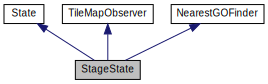
\includegraphics[width=145pt]{classStageState__inherit__graph}
\end{center}
\end{figure}


Diagrama de colaboração para Stage\+State\+:\nopagebreak
\begin{figure}[H]
\begin{center}
\leavevmode
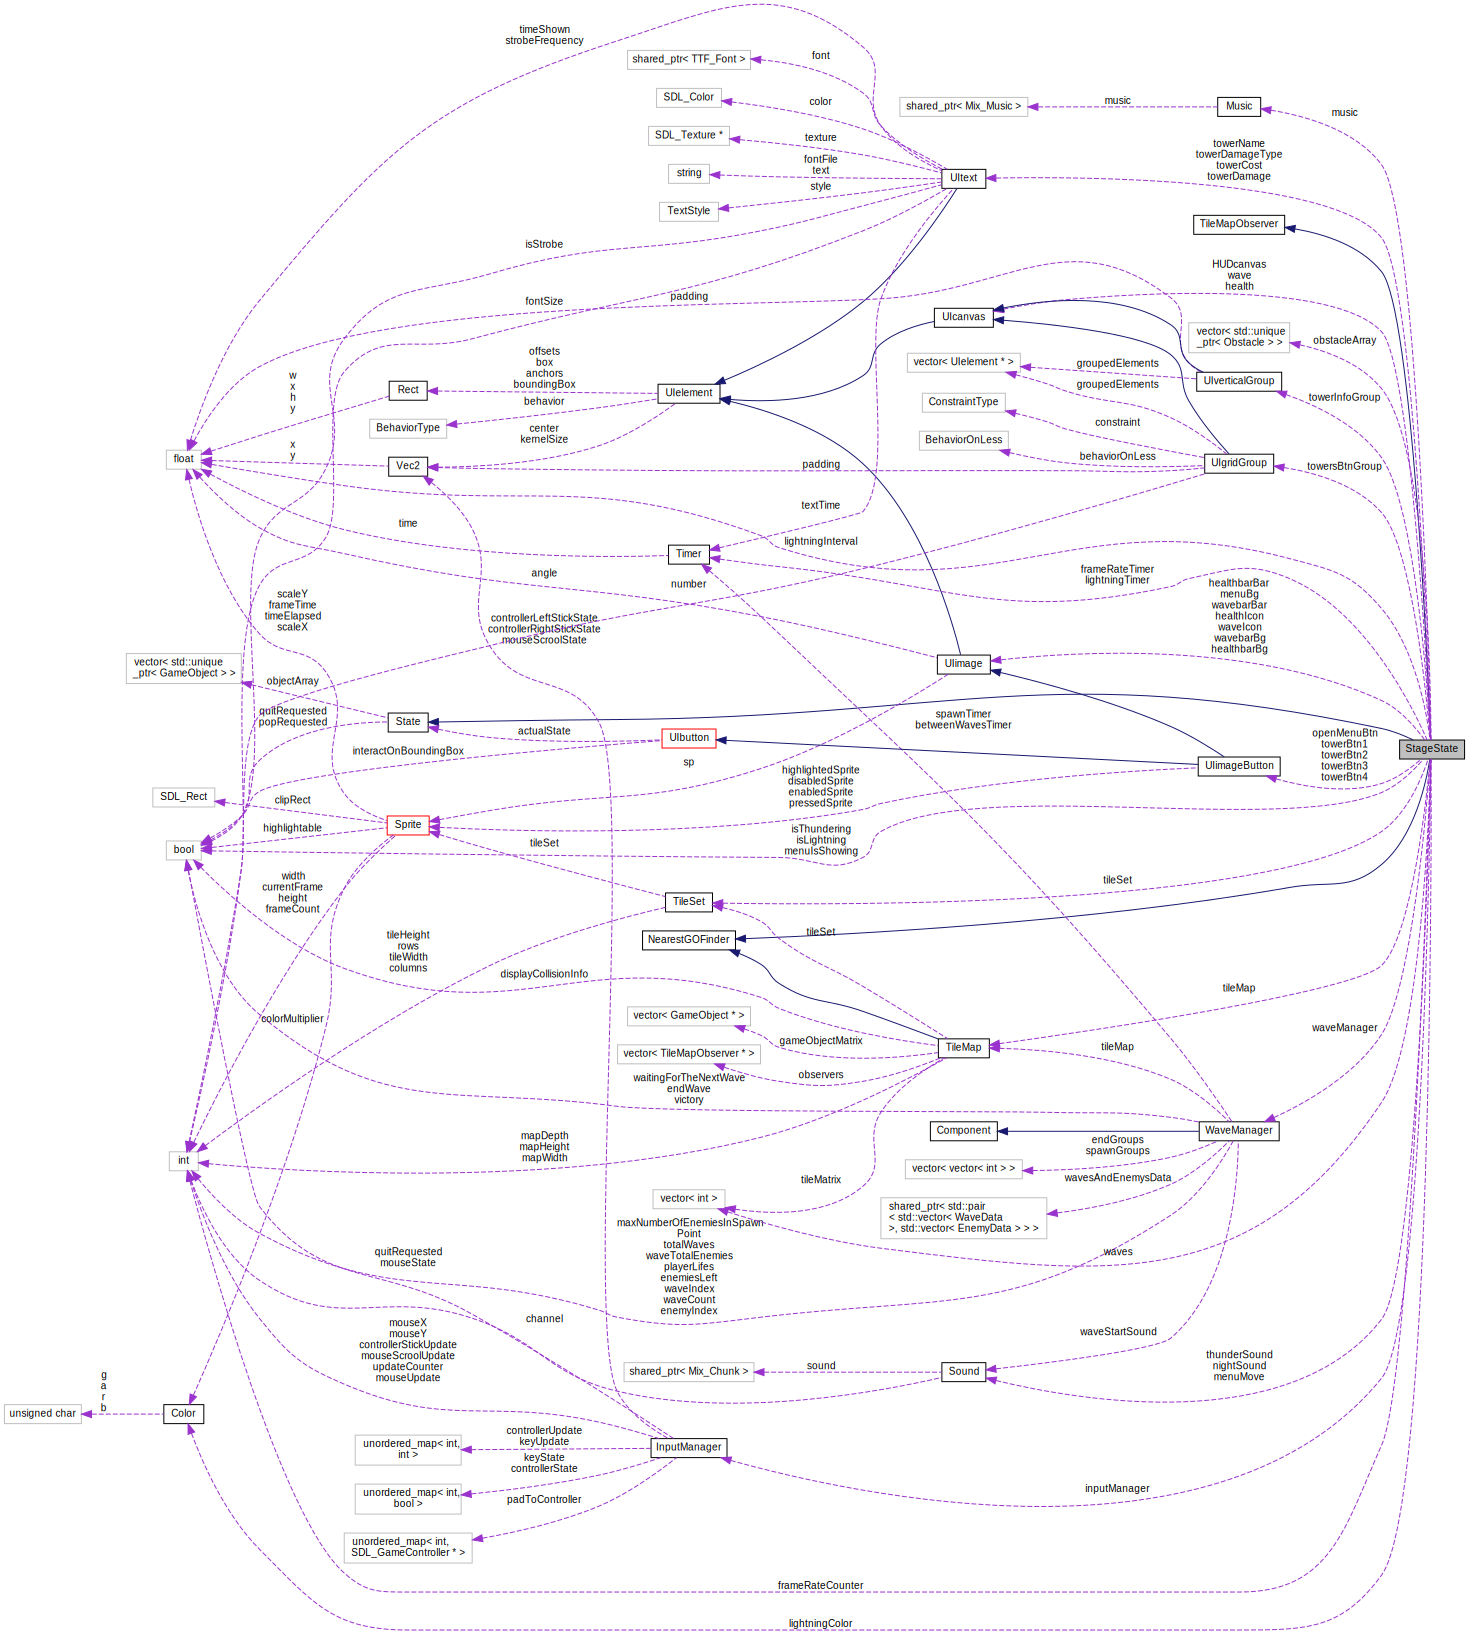
\includegraphics[width=350pt]{classStageState__coll__graph}
\end{center}
\end{figure}
\subsection*{Métodos Públicos}
\begin{DoxyCompactItemize}
\item 
\hyperlink{classStageState_a83447a9a485bd3cf9f2c0d293343ec42}{Stage\+State} (void)
\item 
\hyperlink{classStageState_aaf42c9072c4d2503c8566135ef2a10da}{$\sim$\+Stage\+State} (void)
\item 
void \hyperlink{classStageState_ae77d7d804ee36c434faf52ace163e85a}{Update} (float dt)
\item 
void \hyperlink{classStageState_a6539a58d85b9367d6c027c3348f1b538}{Render} (void) const 
\item 
void \hyperlink{classStageState_a7551ce8a236840e075f6f38f44140e59}{Pause} (void)
\item 
void \hyperlink{classStageState_a1ca42c08929c560284b04a08362e0c8c}{Resume} (void)
\end{DoxyCompactItemize}
\subsection*{Métodos Privados}
\begin{DoxyCompactItemize}
\item 
void \hyperlink{classStageState_a4d8a6aaeb5c87f9cd829ad10825ce06f}{Create\+Alien} ()
\end{DoxyCompactItemize}
\subsection*{Atributos Privados}
\begin{DoxyCompactItemize}
\item 
\hyperlink{classSprite}{Sprite} \hyperlink{classStageState_aa52c55dee219d1bbd1690e8c3c8e34f6}{bg}
\item 
\hyperlink{classTileMap}{Tile\+Map} $\ast$ \hyperlink{classStageState_a1c795e4b3e5c0522709a6060e52291e4}{tile\+Map}
\item 
\hyperlink{classTileSet}{Tile\+Set} \hyperlink{classStageState_ac1ef17645d0585767eaf96693a88d9bb}{tile\+Set}
\item 
\hyperlink{classInputManager}{Input\+Manager} \& \hyperlink{classStageState_acbf7ba483ee1ae6fe7d20f22b5c721b3}{input\+Manager}
\item 
\hyperlink{classMusic}{Music} \hyperlink{classStageState_a60c8325a1df466aff9f24ea167178350}{music}
\end{DoxyCompactItemize}
\subsection*{Additional Inherited Members}


\subsection{Construtores \& Destrutores}
\hypertarget{classStageState_a83447a9a485bd3cf9f2c0d293343ec42}{\index{Stage\+State@{Stage\+State}!Stage\+State@{Stage\+State}}
\index{Stage\+State@{Stage\+State}!Stage\+State@{Stage\+State}}
\subsubsection[{Stage\+State}]{\setlength{\rightskip}{0pt plus 5cm}Stage\+State\+::\+Stage\+State (
\begin{DoxyParamCaption}
\item[{void}]{}
\end{DoxyParamCaption}
)}}\label{classStageState_a83447a9a485bd3cf9f2c0d293343ec42}
\hypertarget{classStageState_aaf42c9072c4d2503c8566135ef2a10da}{\index{Stage\+State@{Stage\+State}!````~Stage\+State@{$\sim$\+Stage\+State}}
\index{````~Stage\+State@{$\sim$\+Stage\+State}!Stage\+State@{Stage\+State}}
\subsubsection[{$\sim$\+Stage\+State}]{\setlength{\rightskip}{0pt plus 5cm}Stage\+State\+::$\sim$\+Stage\+State (
\begin{DoxyParamCaption}
\item[{void}]{}
\end{DoxyParamCaption}
)}}\label{classStageState_aaf42c9072c4d2503c8566135ef2a10da}


\subsection{Métodos}
\hypertarget{classStageState_a4d8a6aaeb5c87f9cd829ad10825ce06f}{\index{Stage\+State@{Stage\+State}!Create\+Alien@{Create\+Alien}}
\index{Create\+Alien@{Create\+Alien}!Stage\+State@{Stage\+State}}
\subsubsection[{Create\+Alien}]{\setlength{\rightskip}{0pt plus 5cm}void Stage\+State\+::\+Create\+Alien (
\begin{DoxyParamCaption}
\item[{void}]{}
\end{DoxyParamCaption}
)\hspace{0.3cm}{\ttfamily [private]}}}\label{classStageState_a4d8a6aaeb5c87f9cd829ad10825ce06f}
\hypertarget{classStageState_a7551ce8a236840e075f6f38f44140e59}{\index{Stage\+State@{Stage\+State}!Pause@{Pause}}
\index{Pause@{Pause}!Stage\+State@{Stage\+State}}
\subsubsection[{Pause}]{\setlength{\rightskip}{0pt plus 5cm}void Stage\+State\+::\+Pause (
\begin{DoxyParamCaption}
\item[{void}]{}
\end{DoxyParamCaption}
)\hspace{0.3cm}{\ttfamily [virtual]}}}\label{classStageState_a7551ce8a236840e075f6f38f44140e59}


Implementa \hyperlink{classState_ae9fa377b30f06fdd809a1557bfbc190a}{State}.

\hypertarget{classStageState_a6539a58d85b9367d6c027c3348f1b538}{\index{Stage\+State@{Stage\+State}!Render@{Render}}
\index{Render@{Render}!Stage\+State@{Stage\+State}}
\subsubsection[{Render}]{\setlength{\rightskip}{0pt plus 5cm}void Stage\+State\+::\+Render (
\begin{DoxyParamCaption}
\item[{void}]{}
\end{DoxyParamCaption}
) const\hspace{0.3cm}{\ttfamily [virtual]}}}\label{classStageState_a6539a58d85b9367d6c027c3348f1b538}


Implementa \hyperlink{classState_ad1f023e61676d0cef92afbaba48ec7ca}{State}.

\hypertarget{classStageState_a1ca42c08929c560284b04a08362e0c8c}{\index{Stage\+State@{Stage\+State}!Resume@{Resume}}
\index{Resume@{Resume}!Stage\+State@{Stage\+State}}
\subsubsection[{Resume}]{\setlength{\rightskip}{0pt plus 5cm}void Stage\+State\+::\+Resume (
\begin{DoxyParamCaption}
\item[{void}]{}
\end{DoxyParamCaption}
)\hspace{0.3cm}{\ttfamily [virtual]}}}\label{classStageState_a1ca42c08929c560284b04a08362e0c8c}


Implementa \hyperlink{classState_ac6d3f8b50530eec89e1344bab93f1006}{State}.

\hypertarget{classStageState_ae77d7d804ee36c434faf52ace163e85a}{\index{Stage\+State@{Stage\+State}!Update@{Update}}
\index{Update@{Update}!Stage\+State@{Stage\+State}}
\subsubsection[{Update}]{\setlength{\rightskip}{0pt plus 5cm}void Stage\+State\+::\+Update (
\begin{DoxyParamCaption}
\item[{float}]{dt}
\end{DoxyParamCaption}
)\hspace{0.3cm}{\ttfamily [virtual]}}}\label{classStageState_ae77d7d804ee36c434faf52ace163e85a}


Implementa \hyperlink{classState_ad79561dfb4e1a6b722a3d9c84b06e91c}{State}.



\subsection{Atributos}
\hypertarget{classStageState_aa52c55dee219d1bbd1690e8c3c8e34f6}{\index{Stage\+State@{Stage\+State}!bg@{bg}}
\index{bg@{bg}!Stage\+State@{Stage\+State}}
\subsubsection[{bg}]{\setlength{\rightskip}{0pt plus 5cm}{\bf Sprite} Stage\+State\+::bg\hspace{0.3cm}{\ttfamily [private]}}}\label{classStageState_aa52c55dee219d1bbd1690e8c3c8e34f6}
\hypertarget{classStageState_acbf7ba483ee1ae6fe7d20f22b5c721b3}{\index{Stage\+State@{Stage\+State}!input\+Manager@{input\+Manager}}
\index{input\+Manager@{input\+Manager}!Stage\+State@{Stage\+State}}
\subsubsection[{input\+Manager}]{\setlength{\rightskip}{0pt plus 5cm}{\bf Input\+Manager}\& Stage\+State\+::input\+Manager\hspace{0.3cm}{\ttfamily [private]}}}\label{classStageState_acbf7ba483ee1ae6fe7d20f22b5c721b3}
\hypertarget{classStageState_a60c8325a1df466aff9f24ea167178350}{\index{Stage\+State@{Stage\+State}!music@{music}}
\index{music@{music}!Stage\+State@{Stage\+State}}
\subsubsection[{music}]{\setlength{\rightskip}{0pt plus 5cm}{\bf Music} Stage\+State\+::music\hspace{0.3cm}{\ttfamily [private]}}}\label{classStageState_a60c8325a1df466aff9f24ea167178350}
\hypertarget{classStageState_a1c795e4b3e5c0522709a6060e52291e4}{\index{Stage\+State@{Stage\+State}!tile\+Map@{tile\+Map}}
\index{tile\+Map@{tile\+Map}!Stage\+State@{Stage\+State}}
\subsubsection[{tile\+Map}]{\setlength{\rightskip}{0pt plus 5cm}{\bf Tile\+Map}$\ast$ Stage\+State\+::tile\+Map\hspace{0.3cm}{\ttfamily [private]}}}\label{classStageState_a1c795e4b3e5c0522709a6060e52291e4}
\hypertarget{classStageState_ac1ef17645d0585767eaf96693a88d9bb}{\index{Stage\+State@{Stage\+State}!tile\+Set@{tile\+Set}}
\index{tile\+Set@{tile\+Set}!Stage\+State@{Stage\+State}}
\subsubsection[{tile\+Set}]{\setlength{\rightskip}{0pt plus 5cm}{\bf Tile\+Set} Stage\+State\+::tile\+Set\hspace{0.3cm}{\ttfamily [private]}}}\label{classStageState_ac1ef17645d0585767eaf96693a88d9bb}


A documentação para esta classe foi gerada a partir dos seguintes arquivos\+:\begin{DoxyCompactItemize}
\item 
Game/include/\hyperlink{StageState_8h}{Stage\+State.\+h}\item 
Game/src/\hyperlink{StageState_8cpp}{Stage\+State.\+cpp}\end{DoxyCompactItemize}

\hypertarget{classState}{\section{Referência da Classe State}
\label{classState}\index{State@{State}}
}


{\ttfamily \#include $<$State.\+h$>$}



Diagrama de Hierarquia para State\+:\nopagebreak
\begin{figure}[H]
\begin{center}
\leavevmode
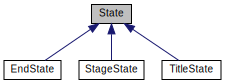
\includegraphics[width=297pt]{classState__inherit__graph}
\end{center}
\end{figure}


Diagrama de colaboração para State\+:
\nopagebreak
\begin{figure}[H]
\begin{center}
\leavevmode
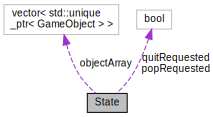
\includegraphics[width=286pt]{classState__coll__graph}
\end{center}
\end{figure}
\subsection*{Métodos Públicos}
\begin{DoxyCompactItemize}
\item 
\hyperlink{classState_aef73d18751fc737c6b4f0893660a0d81}{State} (void)
\item 
virtual \hyperlink{classState_a42d951e307f5b6d1966e15f417cc4101}{$\sim$\+State} (void)
\item 
virtual void \hyperlink{classState_ad79561dfb4e1a6b722a3d9c84b06e91c}{Update} (float dt)=0
\item 
virtual void \hyperlink{classState_ad1f023e61676d0cef92afbaba48ec7ca}{Render} (void) const =0
\item 
virtual void \hyperlink{classState_ae9fa377b30f06fdd809a1557bfbc190a}{Pause} (void)=0
\item 
virtual void \hyperlink{classState_ac6d3f8b50530eec89e1344bab93f1006}{Resume} (void)=0
\item 
virtual void \hyperlink{classState_a431d5f711e028c788a9fdccaf99ff74e}{Add\+Object} (\hyperlink{classGameObject}{Game\+Object} $\ast$object)
\item 
bool \hyperlink{classState_af898168550c4a26b71e4f9ddb0e1f338}{Pop\+Requested} (void)
\item 
bool \hyperlink{classState_a1645048aadaadad50404ff1868e11bb2}{Quit\+Requested} (void)
\end{DoxyCompactItemize}
\subsection*{Métodos Protegidos}
\begin{DoxyCompactItemize}
\item 
virtual void \hyperlink{classState_abb605ec5fe585d227fbf267e0e6c80a9}{Update\+Array} (float dt)
\item 
virtual void \hyperlink{classState_a9a7458d8c801f4d02fd1732a300c8b97}{Render\+Array} (void)
\end{DoxyCompactItemize}
\subsection*{Atributos Protegidos}
\begin{DoxyCompactItemize}
\item 
bool \hyperlink{classState_a9d7c1082cc6592646acec05a6e46f145}{pop\+Requested}
\item 
bool \hyperlink{classState_aa96884ddc05e8f23841298af662ae733}{quit\+Requested}
\item 
std\+::vector$<$ std\+::unique\+\_\+ptr\\*
$<$ \hyperlink{classGameObject}{Game\+Object} $>$ $>$ \hyperlink{classState_a08eaf3c9720d7f90ce579630ca938687}{object\+Array}
\end{DoxyCompactItemize}


\subsection{Construtores \& Destrutores}
\hypertarget{classState_aef73d18751fc737c6b4f0893660a0d81}{\index{State@{State}!State@{State}}
\index{State@{State}!State@{State}}
\subsubsection[{State}]{\setlength{\rightskip}{0pt plus 5cm}State\+::\+State (
\begin{DoxyParamCaption}
\item[{void}]{}
\end{DoxyParamCaption}
)}}\label{classState_aef73d18751fc737c6b4f0893660a0d81}
\hypertarget{classState_a42d951e307f5b6d1966e15f417cc4101}{\index{State@{State}!````~State@{$\sim$\+State}}
\index{````~State@{$\sim$\+State}!State@{State}}
\subsubsection[{$\sim$\+State}]{\setlength{\rightskip}{0pt plus 5cm}State\+::$\sim$\+State (
\begin{DoxyParamCaption}
\item[{void}]{}
\end{DoxyParamCaption}
)\hspace{0.3cm}{\ttfamily [virtual]}}}\label{classState_a42d951e307f5b6d1966e15f417cc4101}


\subsection{Métodos}
\hypertarget{classState_a431d5f711e028c788a9fdccaf99ff74e}{\index{State@{State}!Add\+Object@{Add\+Object}}
\index{Add\+Object@{Add\+Object}!State@{State}}
\subsubsection[{Add\+Object}]{\setlength{\rightskip}{0pt plus 5cm}void State\+::\+Add\+Object (
\begin{DoxyParamCaption}
\item[{{\bf Game\+Object} $\ast$}]{object}
\end{DoxyParamCaption}
)\hspace{0.3cm}{\ttfamily [virtual]}}}\label{classState_a431d5f711e028c788a9fdccaf99ff74e}
\hypertarget{classState_ae9fa377b30f06fdd809a1557bfbc190a}{\index{State@{State}!Pause@{Pause}}
\index{Pause@{Pause}!State@{State}}
\subsubsection[{Pause}]{\setlength{\rightskip}{0pt plus 5cm}virtual void State\+::\+Pause (
\begin{DoxyParamCaption}
\item[{void}]{}
\end{DoxyParamCaption}
)\hspace{0.3cm}{\ttfamily [pure virtual]}}}\label{classState_ae9fa377b30f06fdd809a1557bfbc190a}


Implementado por \hyperlink{classStageState_a7551ce8a236840e075f6f38f44140e59}{Stage\+State}, \hyperlink{classEndState_ac0cc5426e529a4d8572b38e8a87d2d3e}{End\+State} e \hyperlink{classTitleState_acd67f9c5e70d8aba7cccb6449fa6f383}{Title\+State}.

\hypertarget{classState_af898168550c4a26b71e4f9ddb0e1f338}{\index{State@{State}!Pop\+Requested@{Pop\+Requested}}
\index{Pop\+Requested@{Pop\+Requested}!State@{State}}
\subsubsection[{Pop\+Requested}]{\setlength{\rightskip}{0pt plus 5cm}bool State\+::\+Pop\+Requested (
\begin{DoxyParamCaption}
\item[{void}]{}
\end{DoxyParamCaption}
)}}\label{classState_af898168550c4a26b71e4f9ddb0e1f338}
\hypertarget{classState_a1645048aadaadad50404ff1868e11bb2}{\index{State@{State}!Quit\+Requested@{Quit\+Requested}}
\index{Quit\+Requested@{Quit\+Requested}!State@{State}}
\subsubsection[{Quit\+Requested}]{\setlength{\rightskip}{0pt plus 5cm}bool State\+::\+Quit\+Requested (
\begin{DoxyParamCaption}
\item[{void}]{}
\end{DoxyParamCaption}
)}}\label{classState_a1645048aadaadad50404ff1868e11bb2}
\hypertarget{classState_ad1f023e61676d0cef92afbaba48ec7ca}{\index{State@{State}!Render@{Render}}
\index{Render@{Render}!State@{State}}
\subsubsection[{Render}]{\setlength{\rightskip}{0pt plus 5cm}virtual void State\+::\+Render (
\begin{DoxyParamCaption}
\item[{void}]{}
\end{DoxyParamCaption}
) const\hspace{0.3cm}{\ttfamily [pure virtual]}}}\label{classState_ad1f023e61676d0cef92afbaba48ec7ca}


Implementado por \hyperlink{classStageState_a6539a58d85b9367d6c027c3348f1b538}{Stage\+State}, \hyperlink{classEndState_a1c876f3d062547988ac482f9c84d4b14}{End\+State} e \hyperlink{classTitleState_a5b7c34e4f33459f93e2b9f4bc95d83cf}{Title\+State}.

\hypertarget{classState_a9a7458d8c801f4d02fd1732a300c8b97}{\index{State@{State}!Render\+Array@{Render\+Array}}
\index{Render\+Array@{Render\+Array}!State@{State}}
\subsubsection[{Render\+Array}]{\setlength{\rightskip}{0pt plus 5cm}void State\+::\+Render\+Array (
\begin{DoxyParamCaption}
\item[{void}]{}
\end{DoxyParamCaption}
)\hspace{0.3cm}{\ttfamily [protected]}, {\ttfamily [virtual]}}}\label{classState_a9a7458d8c801f4d02fd1732a300c8b97}
\hypertarget{classState_ac6d3f8b50530eec89e1344bab93f1006}{\index{State@{State}!Resume@{Resume}}
\index{Resume@{Resume}!State@{State}}
\subsubsection[{Resume}]{\setlength{\rightskip}{0pt plus 5cm}virtual void State\+::\+Resume (
\begin{DoxyParamCaption}
\item[{void}]{}
\end{DoxyParamCaption}
)\hspace{0.3cm}{\ttfamily [pure virtual]}}}\label{classState_ac6d3f8b50530eec89e1344bab93f1006}


Implementado por \hyperlink{classStageState_a1ca42c08929c560284b04a08362e0c8c}{Stage\+State}, \hyperlink{classEndState_a27e54374f84da806d7bd8bfc985d41b9}{End\+State} e \hyperlink{classTitleState_a97e07af49ceb37c838f435f8f12f0ce1}{Title\+State}.

\hypertarget{classState_ad79561dfb4e1a6b722a3d9c84b06e91c}{\index{State@{State}!Update@{Update}}
\index{Update@{Update}!State@{State}}
\subsubsection[{Update}]{\setlength{\rightskip}{0pt plus 5cm}virtual void State\+::\+Update (
\begin{DoxyParamCaption}
\item[{float}]{dt}
\end{DoxyParamCaption}
)\hspace{0.3cm}{\ttfamily [pure virtual]}}}\label{classState_ad79561dfb4e1a6b722a3d9c84b06e91c}


Implementado por \hyperlink{classStageState_ae77d7d804ee36c434faf52ace163e85a}{Stage\+State}, \hyperlink{classEndState_a0fabb275706a8324521ed1e88efda11d}{End\+State} e \hyperlink{classTitleState_a11c14c15e072eff738fd48f3f0b7c1bf}{Title\+State}.

\hypertarget{classState_abb605ec5fe585d227fbf267e0e6c80a9}{\index{State@{State}!Update\+Array@{Update\+Array}}
\index{Update\+Array@{Update\+Array}!State@{State}}
\subsubsection[{Update\+Array}]{\setlength{\rightskip}{0pt plus 5cm}void State\+::\+Update\+Array (
\begin{DoxyParamCaption}
\item[{float}]{dt}
\end{DoxyParamCaption}
)\hspace{0.3cm}{\ttfamily [protected]}, {\ttfamily [virtual]}}}\label{classState_abb605ec5fe585d227fbf267e0e6c80a9}


\subsection{Atributos}
\hypertarget{classState_a08eaf3c9720d7f90ce579630ca938687}{\index{State@{State}!object\+Array@{object\+Array}}
\index{object\+Array@{object\+Array}!State@{State}}
\subsubsection[{object\+Array}]{\setlength{\rightskip}{0pt plus 5cm}std\+::vector$<$std\+::unique\+\_\+ptr$<${\bf Game\+Object}$>$ $>$ State\+::object\+Array\hspace{0.3cm}{\ttfamily [protected]}}}\label{classState_a08eaf3c9720d7f90ce579630ca938687}
\hypertarget{classState_a9d7c1082cc6592646acec05a6e46f145}{\index{State@{State}!pop\+Requested@{pop\+Requested}}
\index{pop\+Requested@{pop\+Requested}!State@{State}}
\subsubsection[{pop\+Requested}]{\setlength{\rightskip}{0pt plus 5cm}bool State\+::pop\+Requested\hspace{0.3cm}{\ttfamily [protected]}}}\label{classState_a9d7c1082cc6592646acec05a6e46f145}
\hypertarget{classState_aa96884ddc05e8f23841298af662ae733}{\index{State@{State}!quit\+Requested@{quit\+Requested}}
\index{quit\+Requested@{quit\+Requested}!State@{State}}
\subsubsection[{quit\+Requested}]{\setlength{\rightskip}{0pt plus 5cm}bool State\+::quit\+Requested\hspace{0.3cm}{\ttfamily [protected]}}}\label{classState_aa96884ddc05e8f23841298af662ae733}


A documentação para esta classe foi gerada a partir dos seguintes arquivos\+:\begin{DoxyCompactItemize}
\item 
Engine/include/\hyperlink{State_8h}{State.\+h}\item 
Engine/src/\hyperlink{State_8cpp}{State.\+cpp}\end{DoxyCompactItemize}

\hypertarget{classStateData}{\section{Referência da Classe State\+Data}
\label{classStateData}\index{State\+Data@{State\+Data}}
}


{\ttfamily \#include $<$State\+Data.\+h$>$}



Diagrama de Hierarquia para State\+Data\+:\nopagebreak
\begin{figure}[H]
\begin{center}
\leavevmode
\includegraphics[width=158pt]{classStateData__inherit__graph}
\end{center}
\end{figure}
\subsection*{Métodos Públicos}
\begin{DoxyCompactItemize}
\item 
virtual bool \hyperlink{classStateData_a63b33546d704a06bf8f9df6b0590eae4}{Is} (\hyperlink{StateData_8h_a11e85d0fc3db733c13a8d9d030471c7d}{State\+Data\+Type} type\+To\+Check) const =0
\end{DoxyCompactItemize}


\subsection{Métodos}
\hypertarget{classStateData_a63b33546d704a06bf8f9df6b0590eae4}{\index{State\+Data@{State\+Data}!Is@{Is}}
\index{Is@{Is}!State\+Data@{State\+Data}}
\subsubsection[{Is}]{\setlength{\rightskip}{0pt plus 5cm}virtual bool State\+Data\+::\+Is (
\begin{DoxyParamCaption}
\item[{{\bf State\+Data\+Type}}]{type\+To\+Check}
\end{DoxyParamCaption}
) const\hspace{0.3cm}{\ttfamily [pure virtual]}}}\label{classStateData_a63b33546d704a06bf8f9df6b0590eae4}


Implementado por \hyperlink{classEndStateData_abce01a73395040307914a4aa62741463}{End\+State\+Data} e \hyperlink{classEndStateData_abce01a73395040307914a4aa62741463}{End\+State\+Data}.



A documentação para esta classe foi gerada a partir do seguinte arquivo\+:\begin{DoxyCompactItemize}
\item 
Engine/include/\hyperlink{StateData_8h}{State\+Data.\+h}\end{DoxyCompactItemize}

\hypertarget{classText}{\section{Referência da Classe Text}
\label{classText}\index{Text@{Text}}
}


{\ttfamily \#include $<$Text.\+h$>$}



Diagrama de colaboração para Text\+:\nopagebreak
\begin{figure}[H]
\begin{center}
\leavevmode
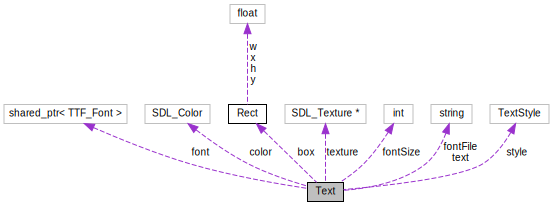
\includegraphics[width=350pt]{classText__coll__graph}
\end{center}
\end{figure}
\subsection*{Métodos Públicos}
\begin{DoxyCompactItemize}
\item 
\hyperlink{classText_ab9d958002beef60e08b0e932267401d0}{Text} (string font\+File, int \hyperlink{classText_af1b0c4c5d94f1a5338398f37e7b9ebbe}{font\+Size}, \hyperlink{Text_8h_ad5957a553b7d89d4921c39cc3ad6bc45}{Text\+Style} \hyperlink{classText_aaf6b429b30c8e7b380aa2433cf1296ea}{style}, S\+D\+L\+\_\+\+Color \hyperlink{classText_ab0f771bd18d8e968f7aaee4a4e26e385}{color}, int x=0, int y=0)
\item 
\hyperlink{classText_a2d49e5c280e205125b149f7777ae30c7}{$\sim$\+Text} ()
\item 
void \hyperlink{classText_af32d96322e20f25f1a4ee99369d08a95}{Render} (int Camera\+X=0, int camera\+Y=0) const 
\item 
void \hyperlink{classText_a8c1865b3d0971b3611ae82e9ad85acb1}{Set\+Pos} (int x, int y, bool center\+X=false, bool center\+Y=false)
\item 
void \hyperlink{classText_abffaafcd871424690014ca0a74c45989}{Set\+Text} (string \hyperlink{classText_a7da8331e2da684bb0485a3ee7893b415}{text})
\item 
void \hyperlink{classText_a16b351605f583b6ece8c93fc8c4df279}{Set\+Color} (S\+D\+L\+\_\+\+Color \hyperlink{classText_ab0f771bd18d8e968f7aaee4a4e26e385}{color})
\item 
void \hyperlink{classText_acd7cd539df681365587e86144cc3c352}{Set\+Style} (\hyperlink{Text_8h_ad5957a553b7d89d4921c39cc3ad6bc45}{Text\+Style} \hyperlink{classText_aaf6b429b30c8e7b380aa2433cf1296ea}{style})
\item 
void \hyperlink{classText_a0d37b9c067e62e10ebd1f0f74dbb5e66}{Set\+Font\+Size} (int \hyperlink{classText_af1b0c4c5d94f1a5338398f37e7b9ebbe}{font\+Size})
\item 
\hyperlink{classVec2}{Vec2} \hyperlink{classText_aa2a449375e15e6abb2911fff0af26c66}{Get\+Size} (void) const 
\end{DoxyCompactItemize}
\subsection*{Métodos Privados}
\begin{DoxyCompactItemize}
\item 
void \hyperlink{classText_a5c794eef4ba7e0bd09a3039835f30e48}{Remake\+Texture} (void)
\end{DoxyCompactItemize}
\subsection*{Atributos Privados}
\begin{DoxyCompactItemize}
\item 
std\+::shared\+\_\+ptr$<$ T\+T\+F\+\_\+\+Font $>$ \hyperlink{classText_a7c89817e7e1d08584cf1b51106ce5ba4}{font}
\item 
S\+D\+L\+\_\+\+Texture $\ast$ \hyperlink{classText_aea2a82ef1d8b4d448b6b3e524bce2cc2}{texture}
\item 
string \hyperlink{classText_a7da8331e2da684bb0485a3ee7893b415}{text}
\item 
\hyperlink{Text_8h_ad5957a553b7d89d4921c39cc3ad6bc45}{Text\+Style} \hyperlink{classText_aaf6b429b30c8e7b380aa2433cf1296ea}{style}
\item 
int \hyperlink{classText_af1b0c4c5d94f1a5338398f37e7b9ebbe}{font\+Size}
\item 
S\+D\+L\+\_\+\+Color \hyperlink{classText_ab0f771bd18d8e968f7aaee4a4e26e385}{color}
\item 
\hyperlink{classRect}{Rect} \hyperlink{classText_a1a2dd837322b9adcd3a2a98f68e633c9}{box}
\end{DoxyCompactItemize}


\subsection{Construtores \& Destrutores}
\hypertarget{classText_ab9d958002beef60e08b0e932267401d0}{\index{Text@{Text}!Text@{Text}}
\index{Text@{Text}!Text@{Text}}
\subsubsection[{Text}]{\setlength{\rightskip}{0pt plus 5cm}Text\+::\+Text (
\begin{DoxyParamCaption}
\item[{string}]{font\+File, }
\item[{int}]{font\+Size, }
\item[{{\bf Text\+Style}}]{style, }
\item[{S\+D\+L\+\_\+\+Color}]{color, }
\item[{int}]{x = {\ttfamily 0}, }
\item[{int}]{y = {\ttfamily 0}}
\end{DoxyParamCaption}
)}}\label{classText_ab9d958002beef60e08b0e932267401d0}
\hypertarget{classText_a2d49e5c280e205125b149f7777ae30c7}{\index{Text@{Text}!````~Text@{$\sim$\+Text}}
\index{````~Text@{$\sim$\+Text}!Text@{Text}}
\subsubsection[{$\sim$\+Text}]{\setlength{\rightskip}{0pt plus 5cm}Text\+::$\sim$\+Text (
\begin{DoxyParamCaption}
{}
\end{DoxyParamCaption}
)}}\label{classText_a2d49e5c280e205125b149f7777ae30c7}


\subsection{Métodos}
\hypertarget{classText_aa2a449375e15e6abb2911fff0af26c66}{\index{Text@{Text}!Get\+Size@{Get\+Size}}
\index{Get\+Size@{Get\+Size}!Text@{Text}}
\subsubsection[{Get\+Size}]{\setlength{\rightskip}{0pt plus 5cm}{\bf Vec2} Text\+::\+Get\+Size (
\begin{DoxyParamCaption}
\item[{void}]{}
\end{DoxyParamCaption}
) const}}\label{classText_aa2a449375e15e6abb2911fff0af26c66}
\hypertarget{classText_a5c794eef4ba7e0bd09a3039835f30e48}{\index{Text@{Text}!Remake\+Texture@{Remake\+Texture}}
\index{Remake\+Texture@{Remake\+Texture}!Text@{Text}}
\subsubsection[{Remake\+Texture}]{\setlength{\rightskip}{0pt plus 5cm}void Text\+::\+Remake\+Texture (
\begin{DoxyParamCaption}
\item[{void}]{}
\end{DoxyParamCaption}
)\hspace{0.3cm}{\ttfamily [private]}}}\label{classText_a5c794eef4ba7e0bd09a3039835f30e48}
\hypertarget{classText_af32d96322e20f25f1a4ee99369d08a95}{\index{Text@{Text}!Render@{Render}}
\index{Render@{Render}!Text@{Text}}
\subsubsection[{Render}]{\setlength{\rightskip}{0pt plus 5cm}void Text\+::\+Render (
\begin{DoxyParamCaption}
\item[{int}]{Camera\+X = {\ttfamily 0}, }
\item[{int}]{camera\+Y = {\ttfamily 0}}
\end{DoxyParamCaption}
) const}}\label{classText_af32d96322e20f25f1a4ee99369d08a95}
\hypertarget{classText_a16b351605f583b6ece8c93fc8c4df279}{\index{Text@{Text}!Set\+Color@{Set\+Color}}
\index{Set\+Color@{Set\+Color}!Text@{Text}}
\subsubsection[{Set\+Color}]{\setlength{\rightskip}{0pt plus 5cm}void Text\+::\+Set\+Color (
\begin{DoxyParamCaption}
\item[{S\+D\+L\+\_\+\+Color}]{color}
\end{DoxyParamCaption}
)}}\label{classText_a16b351605f583b6ece8c93fc8c4df279}
\hypertarget{classText_a0d37b9c067e62e10ebd1f0f74dbb5e66}{\index{Text@{Text}!Set\+Font\+Size@{Set\+Font\+Size}}
\index{Set\+Font\+Size@{Set\+Font\+Size}!Text@{Text}}
\subsubsection[{Set\+Font\+Size}]{\setlength{\rightskip}{0pt plus 5cm}void Text\+::\+Set\+Font\+Size (
\begin{DoxyParamCaption}
\item[{int}]{font\+Size}
\end{DoxyParamCaption}
)}}\label{classText_a0d37b9c067e62e10ebd1f0f74dbb5e66}
\hypertarget{classText_a8c1865b3d0971b3611ae82e9ad85acb1}{\index{Text@{Text}!Set\+Pos@{Set\+Pos}}
\index{Set\+Pos@{Set\+Pos}!Text@{Text}}
\subsubsection[{Set\+Pos}]{\setlength{\rightskip}{0pt plus 5cm}void Text\+::\+Set\+Pos (
\begin{DoxyParamCaption}
\item[{int}]{x, }
\item[{int}]{y, }
\item[{bool}]{center\+X = {\ttfamily false}, }
\item[{bool}]{center\+Y = {\ttfamily false}}
\end{DoxyParamCaption}
)}}\label{classText_a8c1865b3d0971b3611ae82e9ad85acb1}
\hypertarget{classText_acd7cd539df681365587e86144cc3c352}{\index{Text@{Text}!Set\+Style@{Set\+Style}}
\index{Set\+Style@{Set\+Style}!Text@{Text}}
\subsubsection[{Set\+Style}]{\setlength{\rightskip}{0pt plus 5cm}void Text\+::\+Set\+Style (
\begin{DoxyParamCaption}
\item[{{\bf Text\+Style}}]{style}
\end{DoxyParamCaption}
)}}\label{classText_acd7cd539df681365587e86144cc3c352}
\hypertarget{classText_abffaafcd871424690014ca0a74c45989}{\index{Text@{Text}!Set\+Text@{Set\+Text}}
\index{Set\+Text@{Set\+Text}!Text@{Text}}
\subsubsection[{Set\+Text}]{\setlength{\rightskip}{0pt plus 5cm}void Text\+::\+Set\+Text (
\begin{DoxyParamCaption}
\item[{string}]{text}
\end{DoxyParamCaption}
)}}\label{classText_abffaafcd871424690014ca0a74c45989}


\subsection{Atributos}
\hypertarget{classText_a1a2dd837322b9adcd3a2a98f68e633c9}{\index{Text@{Text}!box@{box}}
\index{box@{box}!Text@{Text}}
\subsubsection[{box}]{\setlength{\rightskip}{0pt plus 5cm}{\bf Rect} Text\+::box\hspace{0.3cm}{\ttfamily [private]}}}\label{classText_a1a2dd837322b9adcd3a2a98f68e633c9}
\hypertarget{classText_ab0f771bd18d8e968f7aaee4a4e26e385}{\index{Text@{Text}!color@{color}}
\index{color@{color}!Text@{Text}}
\subsubsection[{color}]{\setlength{\rightskip}{0pt plus 5cm}S\+D\+L\+\_\+\+Color Text\+::color\hspace{0.3cm}{\ttfamily [private]}}}\label{classText_ab0f771bd18d8e968f7aaee4a4e26e385}
\hypertarget{classText_a7c89817e7e1d08584cf1b51106ce5ba4}{\index{Text@{Text}!font@{font}}
\index{font@{font}!Text@{Text}}
\subsubsection[{font}]{\setlength{\rightskip}{0pt plus 5cm}std\+::shared\+\_\+ptr$<$T\+T\+F\+\_\+\+Font$>$ Text\+::font\hspace{0.3cm}{\ttfamily [private]}}}\label{classText_a7c89817e7e1d08584cf1b51106ce5ba4}
\hypertarget{classText_af1b0c4c5d94f1a5338398f37e7b9ebbe}{\index{Text@{Text}!font\+Size@{font\+Size}}
\index{font\+Size@{font\+Size}!Text@{Text}}
\subsubsection[{font\+Size}]{\setlength{\rightskip}{0pt plus 5cm}int Text\+::font\+Size\hspace{0.3cm}{\ttfamily [private]}}}\label{classText_af1b0c4c5d94f1a5338398f37e7b9ebbe}
\hypertarget{classText_aaf6b429b30c8e7b380aa2433cf1296ea}{\index{Text@{Text}!style@{style}}
\index{style@{style}!Text@{Text}}
\subsubsection[{style}]{\setlength{\rightskip}{0pt plus 5cm}{\bf Text\+Style} Text\+::style\hspace{0.3cm}{\ttfamily [private]}}}\label{classText_aaf6b429b30c8e7b380aa2433cf1296ea}
\hypertarget{classText_a7da8331e2da684bb0485a3ee7893b415}{\index{Text@{Text}!text@{text}}
\index{text@{text}!Text@{Text}}
\subsubsection[{text}]{\setlength{\rightskip}{0pt plus 5cm}string Text\+::text\hspace{0.3cm}{\ttfamily [private]}}}\label{classText_a7da8331e2da684bb0485a3ee7893b415}
\hypertarget{classText_aea2a82ef1d8b4d448b6b3e524bce2cc2}{\index{Text@{Text}!texture@{texture}}
\index{texture@{texture}!Text@{Text}}
\subsubsection[{texture}]{\setlength{\rightskip}{0pt plus 5cm}S\+D\+L\+\_\+\+Texture$\ast$ Text\+::texture\hspace{0.3cm}{\ttfamily [private]}}}\label{classText_aea2a82ef1d8b4d448b6b3e524bce2cc2}


A documentação para esta classe foi gerada a partir dos seguintes arquivos\+:\begin{DoxyCompactItemize}
\item 
Engine/include/\hyperlink{Text_8h}{Text.\+h}\item 
Engine/src/\hyperlink{Text_8cpp}{Text.\+cpp}\end{DoxyCompactItemize}

\hypertarget{classTileMap}{\section{Referência da Classe Tile\+Map}
\label{classTileMap}\index{Tile\+Map@{Tile\+Map}}
}


{\ttfamily \#include $<$Tile\+Map.\+h$>$}



Diagrama de colaboração para Tile\+Map\+:
\nopagebreak
\begin{figure}[H]
\begin{center}
\leavevmode
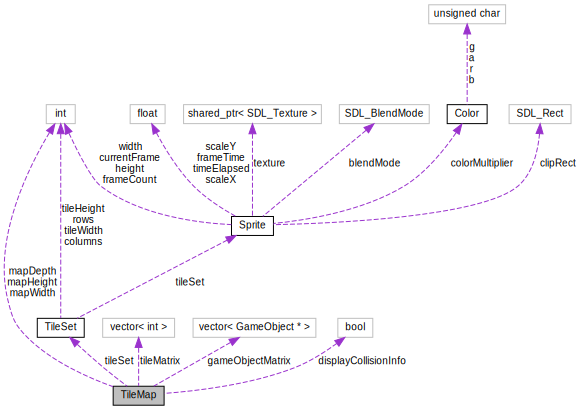
\includegraphics[width=350pt]{classTileMap__coll__graph}
\end{center}
\end{figure}
\subsection*{Métodos Públicos}
\begin{DoxyCompactItemize}
\item 
\hyperlink{classTileMap_acf6fe3a182047153ec9c25fadc55056c}{Tile\+Map} (string file, \hyperlink{classTileSet}{Tile\+Set} $\ast$\hyperlink{classTileMap_a24b2ea7aecfd795f1e13dfa9b0b3cb76}{tile\+Set})
\item 
int \& \hyperlink{classTileMap_a3b8dec192ee9ccca2b4476821235cc0a}{At} (int x, int y, int z=0) const 
\item 
void \hyperlink{classTileMap_a7ec4f6245f0e772c256f5b9240ce67ee}{Render} (int camera\+X=0, int camera\+Y=0) const 
\item 
void \hyperlink{classTileMap_a08748800b6fb6bd307acd3693a39d679}{Render\+Layer} (int layer, int camera\+X=0, int camera\+Y=0) const 
\item 
int \hyperlink{classTileMap_a072dbe1dbd793712baefe154c3058ab2}{Get\+Width} (void) const 
\item 
int \hyperlink{classTileMap_a9fe48260088655aa252b4d40e60f1390}{Get\+Height} (void) const 
\item 
int \hyperlink{classTileMap_aeb8c6a4101e449c33d963041345d918e}{Get\+Depth} (void) const 
\end{DoxyCompactItemize}
\subsection*{Métodos Privados}
\begin{DoxyCompactItemize}
\item 
void \hyperlink{classTileMap_af79b1c89448feb571b799a3642dab5f9}{Load} (string file)
\item 
void \hyperlink{classTileMap_aeaeb5ed2cc7e621ab2fe9f5ee26b2b69}{Set\+Tile\+Set} (\hyperlink{classTileSet}{Tile\+Set} $\ast$\hyperlink{classTileMap_a24b2ea7aecfd795f1e13dfa9b0b3cb76}{tile\+Set})
\item 
int \hyperlink{classTileMap_adda18b2c09dbcc6cfb91b39ae9bee271}{Calculate\+Parallax\+Scrolling} (int num, int camera, int layer) const 
\end{DoxyCompactItemize}
\subsection*{Atributos Privados}
\begin{DoxyCompactItemize}
\item 
std\+::vector$<$ int $>$ \hyperlink{classTileMap_ac1d3ce0587c4e615682b71fd96295e0e}{tile\+Matrix}
\item 
\hyperlink{classTileSet}{Tile\+Set} $\ast$ \hyperlink{classTileMap_a24b2ea7aecfd795f1e13dfa9b0b3cb76}{tile\+Set}
\item 
int \hyperlink{classTileMap_ae2361e840eacaebbbbc91541ded00655}{map\+Width}
\item 
int \hyperlink{classTileMap_a8fec89ca278b51de7f3e38831d9fb161}{map\+Height}
\item 
int \hyperlink{classTileMap_a9f9975834cc5f1acad95d72828858862}{map\+Depth}
\end{DoxyCompactItemize}


\subsection{Construtores \& Destrutores}
\hypertarget{classTileMap_acf6fe3a182047153ec9c25fadc55056c}{\index{Tile\+Map@{Tile\+Map}!Tile\+Map@{Tile\+Map}}
\index{Tile\+Map@{Tile\+Map}!Tile\+Map@{Tile\+Map}}
\subsubsection[{Tile\+Map}]{\setlength{\rightskip}{0pt plus 5cm}Tile\+Map\+::\+Tile\+Map (
\begin{DoxyParamCaption}
\item[{string}]{file, }
\item[{{\bf Tile\+Set} $\ast$}]{tile\+Set}
\end{DoxyParamCaption}
)}}\label{classTileMap_acf6fe3a182047153ec9c25fadc55056c}


\subsection{Métodos}
\hypertarget{classTileMap_a3b8dec192ee9ccca2b4476821235cc0a}{\index{Tile\+Map@{Tile\+Map}!At@{At}}
\index{At@{At}!Tile\+Map@{Tile\+Map}}
\subsubsection[{At}]{\setlength{\rightskip}{0pt plus 5cm}int \& Tile\+Map\+::\+At (
\begin{DoxyParamCaption}
\item[{int}]{x, }
\item[{int}]{y, }
\item[{int}]{z = {\ttfamily 0}}
\end{DoxyParamCaption}
) const}}\label{classTileMap_a3b8dec192ee9ccca2b4476821235cc0a}
\hypertarget{classTileMap_adda18b2c09dbcc6cfb91b39ae9bee271}{\index{Tile\+Map@{Tile\+Map}!Calculate\+Parallax\+Scrolling@{Calculate\+Parallax\+Scrolling}}
\index{Calculate\+Parallax\+Scrolling@{Calculate\+Parallax\+Scrolling}!Tile\+Map@{Tile\+Map}}
\subsubsection[{Calculate\+Parallax\+Scrolling}]{\setlength{\rightskip}{0pt plus 5cm}int Tile\+Map\+::\+Calculate\+Parallax\+Scrolling (
\begin{DoxyParamCaption}
\item[{int}]{num, }
\item[{int}]{camera, }
\item[{int}]{layer}
\end{DoxyParamCaption}
) const\hspace{0.3cm}{\ttfamily [private]}}}\label{classTileMap_adda18b2c09dbcc6cfb91b39ae9bee271}
\hypertarget{classTileMap_aeb8c6a4101e449c33d963041345d918e}{\index{Tile\+Map@{Tile\+Map}!Get\+Depth@{Get\+Depth}}
\index{Get\+Depth@{Get\+Depth}!Tile\+Map@{Tile\+Map}}
\subsubsection[{Get\+Depth}]{\setlength{\rightskip}{0pt plus 5cm}int Tile\+Map\+::\+Get\+Depth (
\begin{DoxyParamCaption}
\item[{void}]{}
\end{DoxyParamCaption}
) const}}\label{classTileMap_aeb8c6a4101e449c33d963041345d918e}
\hypertarget{classTileMap_a9fe48260088655aa252b4d40e60f1390}{\index{Tile\+Map@{Tile\+Map}!Get\+Height@{Get\+Height}}
\index{Get\+Height@{Get\+Height}!Tile\+Map@{Tile\+Map}}
\subsubsection[{Get\+Height}]{\setlength{\rightskip}{0pt plus 5cm}int Tile\+Map\+::\+Get\+Height (
\begin{DoxyParamCaption}
\item[{void}]{}
\end{DoxyParamCaption}
) const}}\label{classTileMap_a9fe48260088655aa252b4d40e60f1390}
\hypertarget{classTileMap_a072dbe1dbd793712baefe154c3058ab2}{\index{Tile\+Map@{Tile\+Map}!Get\+Width@{Get\+Width}}
\index{Get\+Width@{Get\+Width}!Tile\+Map@{Tile\+Map}}
\subsubsection[{Get\+Width}]{\setlength{\rightskip}{0pt plus 5cm}int Tile\+Map\+::\+Get\+Width (
\begin{DoxyParamCaption}
\item[{void}]{}
\end{DoxyParamCaption}
) const}}\label{classTileMap_a072dbe1dbd793712baefe154c3058ab2}
\hypertarget{classTileMap_af79b1c89448feb571b799a3642dab5f9}{\index{Tile\+Map@{Tile\+Map}!Load@{Load}}
\index{Load@{Load}!Tile\+Map@{Tile\+Map}}
\subsubsection[{Load}]{\setlength{\rightskip}{0pt plus 5cm}void Tile\+Map\+::\+Load (
\begin{DoxyParamCaption}
\item[{string}]{file}
\end{DoxyParamCaption}
)\hspace{0.3cm}{\ttfamily [private]}}}\label{classTileMap_af79b1c89448feb571b799a3642dab5f9}
\hypertarget{classTileMap_a7ec4f6245f0e772c256f5b9240ce67ee}{\index{Tile\+Map@{Tile\+Map}!Render@{Render}}
\index{Render@{Render}!Tile\+Map@{Tile\+Map}}
\subsubsection[{Render}]{\setlength{\rightskip}{0pt plus 5cm}void Tile\+Map\+::\+Render (
\begin{DoxyParamCaption}
\item[{int}]{camera\+X = {\ttfamily 0}, }
\item[{int}]{camera\+Y = {\ttfamily 0}}
\end{DoxyParamCaption}
) const}}\label{classTileMap_a7ec4f6245f0e772c256f5b9240ce67ee}
\hypertarget{classTileMap_a08748800b6fb6bd307acd3693a39d679}{\index{Tile\+Map@{Tile\+Map}!Render\+Layer@{Render\+Layer}}
\index{Render\+Layer@{Render\+Layer}!Tile\+Map@{Tile\+Map}}
\subsubsection[{Render\+Layer}]{\setlength{\rightskip}{0pt plus 5cm}void Tile\+Map\+::\+Render\+Layer (
\begin{DoxyParamCaption}
\item[{int}]{layer, }
\item[{int}]{camera\+X = {\ttfamily 0}, }
\item[{int}]{camera\+Y = {\ttfamily 0}}
\end{DoxyParamCaption}
) const}}\label{classTileMap_a08748800b6fb6bd307acd3693a39d679}
\hypertarget{classTileMap_aeaeb5ed2cc7e621ab2fe9f5ee26b2b69}{\index{Tile\+Map@{Tile\+Map}!Set\+Tile\+Set@{Set\+Tile\+Set}}
\index{Set\+Tile\+Set@{Set\+Tile\+Set}!Tile\+Map@{Tile\+Map}}
\subsubsection[{Set\+Tile\+Set}]{\setlength{\rightskip}{0pt plus 5cm}void Tile\+Map\+::\+Set\+Tile\+Set (
\begin{DoxyParamCaption}
\item[{{\bf Tile\+Set} $\ast$}]{tile\+Set}
\end{DoxyParamCaption}
)\hspace{0.3cm}{\ttfamily [private]}}}\label{classTileMap_aeaeb5ed2cc7e621ab2fe9f5ee26b2b69}


\subsection{Atributos}
\hypertarget{classTileMap_a9f9975834cc5f1acad95d72828858862}{\index{Tile\+Map@{Tile\+Map}!map\+Depth@{map\+Depth}}
\index{map\+Depth@{map\+Depth}!Tile\+Map@{Tile\+Map}}
\subsubsection[{map\+Depth}]{\setlength{\rightskip}{0pt plus 5cm}int Tile\+Map\+::map\+Depth\hspace{0.3cm}{\ttfamily [private]}}}\label{classTileMap_a9f9975834cc5f1acad95d72828858862}
\hypertarget{classTileMap_a8fec89ca278b51de7f3e38831d9fb161}{\index{Tile\+Map@{Tile\+Map}!map\+Height@{map\+Height}}
\index{map\+Height@{map\+Height}!Tile\+Map@{Tile\+Map}}
\subsubsection[{map\+Height}]{\setlength{\rightskip}{0pt plus 5cm}int Tile\+Map\+::map\+Height\hspace{0.3cm}{\ttfamily [private]}}}\label{classTileMap_a8fec89ca278b51de7f3e38831d9fb161}
\hypertarget{classTileMap_ae2361e840eacaebbbbc91541ded00655}{\index{Tile\+Map@{Tile\+Map}!map\+Width@{map\+Width}}
\index{map\+Width@{map\+Width}!Tile\+Map@{Tile\+Map}}
\subsubsection[{map\+Width}]{\setlength{\rightskip}{0pt plus 5cm}int Tile\+Map\+::map\+Width\hspace{0.3cm}{\ttfamily [private]}}}\label{classTileMap_ae2361e840eacaebbbbc91541ded00655}
\hypertarget{classTileMap_ac1d3ce0587c4e615682b71fd96295e0e}{\index{Tile\+Map@{Tile\+Map}!tile\+Matrix@{tile\+Matrix}}
\index{tile\+Matrix@{tile\+Matrix}!Tile\+Map@{Tile\+Map}}
\subsubsection[{tile\+Matrix}]{\setlength{\rightskip}{0pt plus 5cm}std\+::vector$<$int$>$ Tile\+Map\+::tile\+Matrix\hspace{0.3cm}{\ttfamily [private]}}}\label{classTileMap_ac1d3ce0587c4e615682b71fd96295e0e}
\hypertarget{classTileMap_a24b2ea7aecfd795f1e13dfa9b0b3cb76}{\index{Tile\+Map@{Tile\+Map}!tile\+Set@{tile\+Set}}
\index{tile\+Set@{tile\+Set}!Tile\+Map@{Tile\+Map}}
\subsubsection[{tile\+Set}]{\setlength{\rightskip}{0pt plus 5cm}{\bf Tile\+Set}$\ast$ Tile\+Map\+::tile\+Set\hspace{0.3cm}{\ttfamily [private]}}}\label{classTileMap_a24b2ea7aecfd795f1e13dfa9b0b3cb76}


A documentação para esta classe foi gerada a partir dos seguintes arquivos\+:\begin{DoxyCompactItemize}
\item 
Engine/include/\hyperlink{TileMap_8h}{Tile\+Map.\+h}\item 
Engine/src/\hyperlink{TileMap_8cpp}{Tile\+Map.\+cpp}\end{DoxyCompactItemize}

\hypertarget{classTileSet}{\section{Referência da Classe Tile\+Set}
\label{classTileSet}\index{Tile\+Set@{Tile\+Set}}
}


{\ttfamily \#include $<$Tileset.\+h$>$}



Diagrama de colaboração para Tile\+Set\+:\nopagebreak
\begin{figure}[H]
\begin{center}
\leavevmode
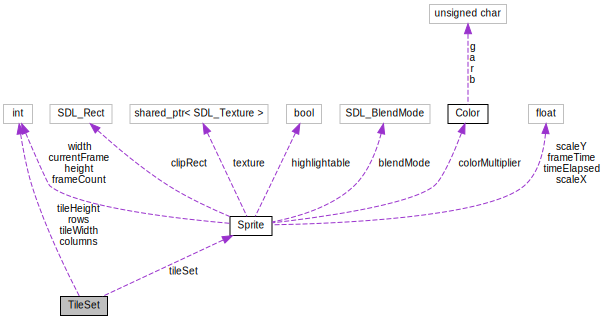
\includegraphics[width=350pt]{classTileSet__coll__graph}
\end{center}
\end{figure}
\subsection*{Métodos Públicos}
\begin{DoxyCompactItemize}
\item 
\hyperlink{classTileSet_a671a1040ef1ba7600a6ea21faa950819}{Tile\+Set} (int \hyperlink{classTileSet_a9ba9087a6da877f78af6cdf9afb0af7c}{tile\+Width}, int \hyperlink{classTileSet_a9409211e1c5560f969b737714be977c0}{tile\+Height}, string file)
\item 
void \hyperlink{classTileSet_a110acfa6e07aa9e5af1798065f23b0f1}{Render} (unsigned int index, float x, float y, bool zoom=true)
\item 
int \hyperlink{classTileSet_a4114a74c06ab5241d904cce67538ae17}{Get\+Tile\+Width} (void)
\item 
int \hyperlink{classTileSet_a965e951eb3ccfd6e318b27c710d973a0}{Get\+Tile\+Height} (void)
\end{DoxyCompactItemize}
\subsection*{Atributos Privados}
\begin{DoxyCompactItemize}
\item 
\hyperlink{classSprite}{Sprite} \hyperlink{classTileSet_adbd7ac102ce306e4f367c32cfa576979}{tile\+Set}
\item 
int \hyperlink{classTileSet_abdfce26ff299e8904107edc22529e28f}{rows}
\item 
int \hyperlink{classTileSet_a47ae11f9d04f9da3fbaba834fdbc62cf}{columns}
\item 
int \hyperlink{classTileSet_a9ba9087a6da877f78af6cdf9afb0af7c}{tile\+Width}
\item 
int \hyperlink{classTileSet_a9409211e1c5560f969b737714be977c0}{tile\+Height}
\end{DoxyCompactItemize}


\subsection{Construtores \& Destrutores}
\hypertarget{classTileSet_a671a1040ef1ba7600a6ea21faa950819}{\index{Tile\+Set@{Tile\+Set}!Tile\+Set@{Tile\+Set}}
\index{Tile\+Set@{Tile\+Set}!Tile\+Set@{Tile\+Set}}
\subsubsection[{Tile\+Set}]{\setlength{\rightskip}{0pt plus 5cm}Tile\+Set\+::\+Tile\+Set (
\begin{DoxyParamCaption}
\item[{int}]{tile\+Width, }
\item[{int}]{tile\+Height, }
\item[{string}]{file}
\end{DoxyParamCaption}
)}}\label{classTileSet_a671a1040ef1ba7600a6ea21faa950819}


\subsection{Métodos}
\hypertarget{classTileSet_a965e951eb3ccfd6e318b27c710d973a0}{\index{Tile\+Set@{Tile\+Set}!Get\+Tile\+Height@{Get\+Tile\+Height}}
\index{Get\+Tile\+Height@{Get\+Tile\+Height}!Tile\+Set@{Tile\+Set}}
\subsubsection[{Get\+Tile\+Height}]{\setlength{\rightskip}{0pt plus 5cm}int Tile\+Set\+::\+Get\+Tile\+Height (
\begin{DoxyParamCaption}
\item[{void}]{}
\end{DoxyParamCaption}
)}}\label{classTileSet_a965e951eb3ccfd6e318b27c710d973a0}
\hypertarget{classTileSet_a4114a74c06ab5241d904cce67538ae17}{\index{Tile\+Set@{Tile\+Set}!Get\+Tile\+Width@{Get\+Tile\+Width}}
\index{Get\+Tile\+Width@{Get\+Tile\+Width}!Tile\+Set@{Tile\+Set}}
\subsubsection[{Get\+Tile\+Width}]{\setlength{\rightskip}{0pt plus 5cm}int Tile\+Set\+::\+Get\+Tile\+Width (
\begin{DoxyParamCaption}
\item[{void}]{}
\end{DoxyParamCaption}
)}}\label{classTileSet_a4114a74c06ab5241d904cce67538ae17}
\hypertarget{classTileSet_a110acfa6e07aa9e5af1798065f23b0f1}{\index{Tile\+Set@{Tile\+Set}!Render@{Render}}
\index{Render@{Render}!Tile\+Set@{Tile\+Set}}
\subsubsection[{Render}]{\setlength{\rightskip}{0pt plus 5cm}void Tile\+Set\+::\+Render (
\begin{DoxyParamCaption}
\item[{unsigned int}]{index, }
\item[{float}]{x, }
\item[{float}]{y, }
\item[{bool}]{zoom = {\ttfamily true}}
\end{DoxyParamCaption}
)}}\label{classTileSet_a110acfa6e07aa9e5af1798065f23b0f1}


\subsection{Atributos}
\hypertarget{classTileSet_a47ae11f9d04f9da3fbaba834fdbc62cf}{\index{Tile\+Set@{Tile\+Set}!columns@{columns}}
\index{columns@{columns}!Tile\+Set@{Tile\+Set}}
\subsubsection[{columns}]{\setlength{\rightskip}{0pt plus 5cm}int Tile\+Set\+::columns\hspace{0.3cm}{\ttfamily [private]}}}\label{classTileSet_a47ae11f9d04f9da3fbaba834fdbc62cf}
\hypertarget{classTileSet_abdfce26ff299e8904107edc22529e28f}{\index{Tile\+Set@{Tile\+Set}!rows@{rows}}
\index{rows@{rows}!Tile\+Set@{Tile\+Set}}
\subsubsection[{rows}]{\setlength{\rightskip}{0pt plus 5cm}int Tile\+Set\+::rows\hspace{0.3cm}{\ttfamily [private]}}}\label{classTileSet_abdfce26ff299e8904107edc22529e28f}
\hypertarget{classTileSet_a9409211e1c5560f969b737714be977c0}{\index{Tile\+Set@{Tile\+Set}!tile\+Height@{tile\+Height}}
\index{tile\+Height@{tile\+Height}!Tile\+Set@{Tile\+Set}}
\subsubsection[{tile\+Height}]{\setlength{\rightskip}{0pt plus 5cm}int Tile\+Set\+::tile\+Height\hspace{0.3cm}{\ttfamily [private]}}}\label{classTileSet_a9409211e1c5560f969b737714be977c0}
\hypertarget{classTileSet_adbd7ac102ce306e4f367c32cfa576979}{\index{Tile\+Set@{Tile\+Set}!tile\+Set@{tile\+Set}}
\index{tile\+Set@{tile\+Set}!Tile\+Set@{Tile\+Set}}
\subsubsection[{tile\+Set}]{\setlength{\rightskip}{0pt plus 5cm}{\bf Sprite} Tile\+Set\+::tile\+Set\hspace{0.3cm}{\ttfamily [private]}}}\label{classTileSet_adbd7ac102ce306e4f367c32cfa576979}
\hypertarget{classTileSet_a9ba9087a6da877f78af6cdf9afb0af7c}{\index{Tile\+Set@{Tile\+Set}!tile\+Width@{tile\+Width}}
\index{tile\+Width@{tile\+Width}!Tile\+Set@{Tile\+Set}}
\subsubsection[{tile\+Width}]{\setlength{\rightskip}{0pt plus 5cm}int Tile\+Set\+::tile\+Width\hspace{0.3cm}{\ttfamily [private]}}}\label{classTileSet_a9ba9087a6da877f78af6cdf9afb0af7c}


A documentação para esta classe foi gerada a partir dos seguintes arquivos\+:\begin{DoxyCompactItemize}
\item 
Engine/include/\hyperlink{Tileset_8h}{Tileset.\+h}\item 
Engine/src/\hyperlink{Tileset_8cpp}{Tileset.\+cpp}\end{DoxyCompactItemize}

\hypertarget{classTimer}{\section{Referência da Classe Timer}
\label{classTimer}\index{Timer@{Timer}}
}


{\ttfamily \#include $<$Timer.\+h$>$}



Diagrama de colaboração para Timer\+:
\nopagebreak
\begin{figure}[H]
\begin{center}
\leavevmode
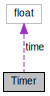
\includegraphics[width=123pt]{classTimer__coll__graph}
\end{center}
\end{figure}
\subsection*{Métodos Públicos}
\begin{DoxyCompactItemize}
\item 
\hyperlink{classTimer_af866f8d58d5ed1da7a0c61df4975be3e}{Timer} (void)
\item 
void \hyperlink{classTimer_aaf9c3b63c5934eb6338f846788262987}{Update} (float dt)
\item 
void \hyperlink{classTimer_abd8c2f405fff4f81f39e651a362b4f60}{Restart} (void)
\item 
float \hyperlink{classTimer_a7d41db026caef9bb0a0a22ddec49dd4c}{Get} (void)
\end{DoxyCompactItemize}
\subsection*{Atributos Privados}
\begin{DoxyCompactItemize}
\item 
float \hyperlink{classTimer_a6c45df1d084a18e41e3a35f6a43df0be}{time}
\end{DoxyCompactItemize}


\subsection{Construtores \& Destrutores}
\hypertarget{classTimer_af866f8d58d5ed1da7a0c61df4975be3e}{\index{Timer@{Timer}!Timer@{Timer}}
\index{Timer@{Timer}!Timer@{Timer}}
\subsubsection[{Timer}]{\setlength{\rightskip}{0pt plus 5cm}Timer\+::\+Timer (
\begin{DoxyParamCaption}
\item[{void}]{}
\end{DoxyParamCaption}
)}}\label{classTimer_af866f8d58d5ed1da7a0c61df4975be3e}


\subsection{Métodos}
\hypertarget{classTimer_a7d41db026caef9bb0a0a22ddec49dd4c}{\index{Timer@{Timer}!Get@{Get}}
\index{Get@{Get}!Timer@{Timer}}
\subsubsection[{Get}]{\setlength{\rightskip}{0pt plus 5cm}float Timer\+::\+Get (
\begin{DoxyParamCaption}
\item[{void}]{}
\end{DoxyParamCaption}
)}}\label{classTimer_a7d41db026caef9bb0a0a22ddec49dd4c}
\hypertarget{classTimer_abd8c2f405fff4f81f39e651a362b4f60}{\index{Timer@{Timer}!Restart@{Restart}}
\index{Restart@{Restart}!Timer@{Timer}}
\subsubsection[{Restart}]{\setlength{\rightskip}{0pt plus 5cm}void Timer\+::\+Restart (
\begin{DoxyParamCaption}
\item[{void}]{}
\end{DoxyParamCaption}
)}}\label{classTimer_abd8c2f405fff4f81f39e651a362b4f60}
\hypertarget{classTimer_aaf9c3b63c5934eb6338f846788262987}{\index{Timer@{Timer}!Update@{Update}}
\index{Update@{Update}!Timer@{Timer}}
\subsubsection[{Update}]{\setlength{\rightskip}{0pt plus 5cm}void Timer\+::\+Update (
\begin{DoxyParamCaption}
\item[{float}]{dt}
\end{DoxyParamCaption}
)}}\label{classTimer_aaf9c3b63c5934eb6338f846788262987}


\subsection{Atributos}
\hypertarget{classTimer_a6c45df1d084a18e41e3a35f6a43df0be}{\index{Timer@{Timer}!time@{time}}
\index{time@{time}!Timer@{Timer}}
\subsubsection[{time}]{\setlength{\rightskip}{0pt plus 5cm}float Timer\+::time\hspace{0.3cm}{\ttfamily [private]}}}\label{classTimer_a6c45df1d084a18e41e3a35f6a43df0be}


A documentação para esta classe foi gerada a partir dos seguintes arquivos\+:\begin{DoxyCompactItemize}
\item 
Engine/include/\hyperlink{Timer_8h}{Timer.\+h}\item 
Engine/src/\hyperlink{Timer_8cpp}{Timer.\+cpp}\end{DoxyCompactItemize}

\hypertarget{classTitleState}{\section{Referência da Classe Title\+State}
\label{classTitleState}\index{Title\+State@{Title\+State}}
}


{\ttfamily \#include $<$Title\+State.\+h$>$}



Diagrama de Hierarquia para Title\+State\+:\nopagebreak
\begin{figure}[H]
\begin{center}
\leavevmode
\includegraphics[width=139pt]{classTitleState__inherit__graph}
\end{center}
\end{figure}


Diagrama de colaboração para Title\+State\+:
\nopagebreak
\begin{figure}[H]
\begin{center}
\leavevmode
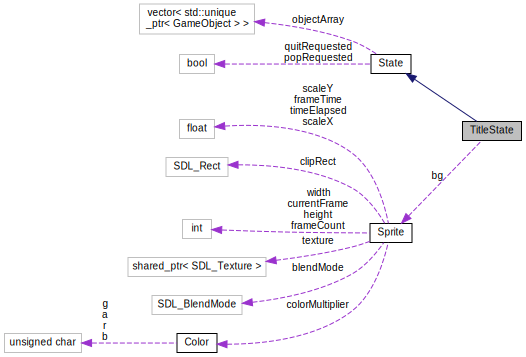
\includegraphics[width=350pt]{classTitleState__coll__graph}
\end{center}
\end{figure}
\subsection*{Métodos Públicos}
\begin{DoxyCompactItemize}
\item 
\hyperlink{classTitleState_a0694f4ac042f6baf1516c26e7385a570}{Title\+State} (void)
\item 
void \hyperlink{classTitleState_a11c14c15e072eff738fd48f3f0b7c1bf}{Update} (float dt)
\item 
void \hyperlink{classTitleState_a5b7c34e4f33459f93e2b9f4bc95d83cf}{Render} (void) const 
\item 
void \hyperlink{classTitleState_acd67f9c5e70d8aba7cccb6449fa6f383}{Pause} (void)
\item 
void \hyperlink{classTitleState_a97e07af49ceb37c838f435f8f12f0ce1}{Resume} (void)
\end{DoxyCompactItemize}
\subsection*{Atributos Privados}
\begin{DoxyCompactItemize}
\item 
\hyperlink{classSprite}{Sprite} \hyperlink{classTitleState_acecffd14c654d7b19636d926579cbe44}{bg}
\end{DoxyCompactItemize}
\subsection*{Additional Inherited Members}


\subsection{Construtores \& Destrutores}
\hypertarget{classTitleState_a0694f4ac042f6baf1516c26e7385a570}{\index{Title\+State@{Title\+State}!Title\+State@{Title\+State}}
\index{Title\+State@{Title\+State}!Title\+State@{Title\+State}}
\subsubsection[{Title\+State}]{\setlength{\rightskip}{0pt plus 5cm}Title\+State\+::\+Title\+State (
\begin{DoxyParamCaption}
\item[{void}]{}
\end{DoxyParamCaption}
)}}\label{classTitleState_a0694f4ac042f6baf1516c26e7385a570}


\subsection{Métodos}
\hypertarget{classTitleState_acd67f9c5e70d8aba7cccb6449fa6f383}{\index{Title\+State@{Title\+State}!Pause@{Pause}}
\index{Pause@{Pause}!Title\+State@{Title\+State}}
\subsubsection[{Pause}]{\setlength{\rightskip}{0pt plus 5cm}void Title\+State\+::\+Pause (
\begin{DoxyParamCaption}
\item[{void}]{}
\end{DoxyParamCaption}
)\hspace{0.3cm}{\ttfamily [virtual]}}}\label{classTitleState_acd67f9c5e70d8aba7cccb6449fa6f383}


Implementa \hyperlink{classState_ae9fa377b30f06fdd809a1557bfbc190a}{State}.

\hypertarget{classTitleState_a5b7c34e4f33459f93e2b9f4bc95d83cf}{\index{Title\+State@{Title\+State}!Render@{Render}}
\index{Render@{Render}!Title\+State@{Title\+State}}
\subsubsection[{Render}]{\setlength{\rightskip}{0pt plus 5cm}void Title\+State\+::\+Render (
\begin{DoxyParamCaption}
\item[{void}]{}
\end{DoxyParamCaption}
) const\hspace{0.3cm}{\ttfamily [virtual]}}}\label{classTitleState_a5b7c34e4f33459f93e2b9f4bc95d83cf}


Implementa \hyperlink{classState_ad1f023e61676d0cef92afbaba48ec7ca}{State}.

\hypertarget{classTitleState_a97e07af49ceb37c838f435f8f12f0ce1}{\index{Title\+State@{Title\+State}!Resume@{Resume}}
\index{Resume@{Resume}!Title\+State@{Title\+State}}
\subsubsection[{Resume}]{\setlength{\rightskip}{0pt plus 5cm}void Title\+State\+::\+Resume (
\begin{DoxyParamCaption}
\item[{void}]{}
\end{DoxyParamCaption}
)\hspace{0.3cm}{\ttfamily [virtual]}}}\label{classTitleState_a97e07af49ceb37c838f435f8f12f0ce1}


Implementa \hyperlink{classState_ac6d3f8b50530eec89e1344bab93f1006}{State}.

\hypertarget{classTitleState_a11c14c15e072eff738fd48f3f0b7c1bf}{\index{Title\+State@{Title\+State}!Update@{Update}}
\index{Update@{Update}!Title\+State@{Title\+State}}
\subsubsection[{Update}]{\setlength{\rightskip}{0pt plus 5cm}void Title\+State\+::\+Update (
\begin{DoxyParamCaption}
\item[{float}]{dt}
\end{DoxyParamCaption}
)\hspace{0.3cm}{\ttfamily [virtual]}}}\label{classTitleState_a11c14c15e072eff738fd48f3f0b7c1bf}


Implementa \hyperlink{classState_ad79561dfb4e1a6b722a3d9c84b06e91c}{State}.



\subsection{Atributos}
\hypertarget{classTitleState_acecffd14c654d7b19636d926579cbe44}{\index{Title\+State@{Title\+State}!bg@{bg}}
\index{bg@{bg}!Title\+State@{Title\+State}}
\subsubsection[{bg}]{\setlength{\rightskip}{0pt plus 5cm}{\bf Sprite} Title\+State\+::bg\hspace{0.3cm}{\ttfamily [private]}}}\label{classTitleState_acecffd14c654d7b19636d926579cbe44}


A documentação para esta classe foi gerada a partir dos seguintes arquivos\+:\begin{DoxyCompactItemize}
\item 
Game/include/\hyperlink{TitleState_8h}{Title\+State.\+h}\item 
Game/src/\hyperlink{TitleState_8cpp}{Title\+State.\+cpp}\end{DoxyCompactItemize}

\hypertarget{classVec2}{\section{Referência da Classe Vec2}
\label{classVec2}\index{Vec2@{Vec2}}
}


{\ttfamily \#include $<$Vec2.\+h$>$}



Diagrama de colaboração para Vec2\+:
\nopagebreak
\begin{figure}[H]
\begin{center}
\leavevmode
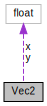
\includegraphics[width=119pt]{classVec2__coll__graph}
\end{center}
\end{figure}
\subsection*{Métodos Públicos}
\begin{DoxyCompactItemize}
\item 
\hyperlink{classVec2_a4e240b8f078ee238e6be681c8d34d759}{Vec2} (void)
\item 
\hyperlink{classVec2_a6256fecebf5a43b14d5d5341c58cfdc4}{Vec2} (float \hyperlink{classVec2_adf8ee322d4b4bcc04146762c018d731f}{x}, float \hyperlink{classVec2_a30543787e62f6d915543cf1dfb04c094}{y})
\item 
\hyperlink{classVec2_ad8309ba4db7467af8c8934e5e0d5751a}{Vec2} (\hyperlink{classVec2}{Vec2} const \&b)
\item 
\hyperlink{classVec2}{Vec2} \hyperlink{classVec2_ac7d3e5daad85a1883eeabb5f6f37fa2c}{operator+} (\hyperlink{classVec2}{Vec2} const \&b) const 
\item 
\hyperlink{classVec2}{Vec2} \hyperlink{classVec2_a5943a96d245b622f13849906296872e8}{operator-\/} (\hyperlink{classVec2}{Vec2} const \&b) const 
\item 
\hyperlink{classVec2}{Vec2} \hyperlink{classVec2_ab8024729f0ff93341ef1826ab264c278}{operator$\ast$} (float b) const 
\item 
\hyperlink{classVec2}{Vec2} \& \hyperlink{classVec2_a5f11bf2c956c09d90d515bbbf46337ec}{operator=} (\hyperlink{classVec2}{Vec2} const \&b)
\item 
\hyperlink{classVec2}{Vec2} \& \hyperlink{classVec2_ae7aa55c56ed024029ee6f450b014dcee}{operator+=} (\hyperlink{classVec2}{Vec2} const \&b)
\item 
\hyperlink{classVec2}{Vec2} \& \hyperlink{classVec2_a04202314b5513694ea805e43bdd754f6}{operator-\/=} (\hyperlink{classVec2}{Vec2} const \&b)
\item 
bool \hyperlink{classVec2_a01d41260f16f9be282347f50f621224b}{operator==} (\hyperlink{classVec2}{Vec2} const \&b) const 
\item 
bool \hyperlink{classVec2_a34b74d6e6cb70aea725c5dc27310eb4a}{operator!=} (\hyperlink{classVec2}{Vec2} const \&b) const 
\item 
\hyperlink{classVec2}{Vec2} \hyperlink{classVec2_a0af80a4efc933b61b2885a815a15a77f}{Member\+Mult} (float const \&b) const 
\item 
float \hyperlink{classVec2_af904886a3658709196f6b171b517f593}{Magnitude} (void) const 
\item 
void \hyperlink{classVec2_ab37a161e393133ba7083d3f9386c0173}{Normalize} (void)
\item 
\hyperlink{classVec2}{Vec2} \hyperlink{classVec2_abb4f9b393a08a4d19c5139a6ba5f5409}{Rotate} (float angle) const 
\item 
float \hyperlink{classVec2_aaf7c998a9f97f4a79e3900289ac566e0}{Distance\+To} (\hyperlink{classVec2}{Vec2} const \&b) const 
\item 
float \hyperlink{classVec2_a416d5d762750e1392139242fdcedb952}{Inclination} (void) const 
\item 
float \hyperlink{classVec2_afdc96d9f65aa822008b9cabc1f571747}{Inclination} (\hyperlink{classVec2}{Vec2} const \&b) const 
\item 
bool \hyperlink{classVec2_a788dc85f57e20be80e85543e6996a4f1}{Is\+In\+Rect} (S\+D\+L\+\_\+\+Rect const \&rect) const 
\item 
void \hyperlink{classVec2_a782588fd0ba59659df8b2a221b58896d}{Set\+Width\+And\+Height} (\hyperlink{classVec2}{Vec2} const \&vec)
\end{DoxyCompactItemize}
\subsection*{Métodos Públicos Estáticos}
\begin{DoxyCompactItemize}
\item 
static \hyperlink{classVec2}{Vec2} \hyperlink{classVec2_ac794548df48539be24dd1e8ebebf8038}{From\+Polar\+Coord} (float magentude, float angle)
\end{DoxyCompactItemize}
\subsection*{Atributos Públicos}
\begin{DoxyCompactItemize}
\item 
float \hyperlink{classVec2_adf8ee322d4b4bcc04146762c018d731f}{x}
\item 
float \hyperlink{classVec2_a30543787e62f6d915543cf1dfb04c094}{y}
\end{DoxyCompactItemize}


\subsection{Construtores \& Destrutores}
\hypertarget{classVec2_a4e240b8f078ee238e6be681c8d34d759}{\index{Vec2@{Vec2}!Vec2@{Vec2}}
\index{Vec2@{Vec2}!Vec2@{Vec2}}
\subsubsection[{Vec2}]{\setlength{\rightskip}{0pt plus 5cm}Vec2\+::\+Vec2 (
\begin{DoxyParamCaption}
\item[{void}]{}
\end{DoxyParamCaption}
)}}\label{classVec2_a4e240b8f078ee238e6be681c8d34d759}
\hypertarget{classVec2_a6256fecebf5a43b14d5d5341c58cfdc4}{\index{Vec2@{Vec2}!Vec2@{Vec2}}
\index{Vec2@{Vec2}!Vec2@{Vec2}}
\subsubsection[{Vec2}]{\setlength{\rightskip}{0pt plus 5cm}Vec2\+::\+Vec2 (
\begin{DoxyParamCaption}
\item[{float}]{x, }
\item[{float}]{y}
\end{DoxyParamCaption}
)}}\label{classVec2_a6256fecebf5a43b14d5d5341c58cfdc4}
\hypertarget{classVec2_ad8309ba4db7467af8c8934e5e0d5751a}{\index{Vec2@{Vec2}!Vec2@{Vec2}}
\index{Vec2@{Vec2}!Vec2@{Vec2}}
\subsubsection[{Vec2}]{\setlength{\rightskip}{0pt plus 5cm}Vec2\+::\+Vec2 (
\begin{DoxyParamCaption}
\item[{{\bf Vec2} const \&}]{b}
\end{DoxyParamCaption}
)}}\label{classVec2_ad8309ba4db7467af8c8934e5e0d5751a}


\subsection{Métodos}
\hypertarget{classVec2_aaf7c998a9f97f4a79e3900289ac566e0}{\index{Vec2@{Vec2}!Distance\+To@{Distance\+To}}
\index{Distance\+To@{Distance\+To}!Vec2@{Vec2}}
\subsubsection[{Distance\+To}]{\setlength{\rightskip}{0pt plus 5cm}float Vec2\+::\+Distance\+To (
\begin{DoxyParamCaption}
\item[{{\bf Vec2} const \&}]{b}
\end{DoxyParamCaption}
) const}}\label{classVec2_aaf7c998a9f97f4a79e3900289ac566e0}
\hypertarget{classVec2_ac794548df48539be24dd1e8ebebf8038}{\index{Vec2@{Vec2}!From\+Polar\+Coord@{From\+Polar\+Coord}}
\index{From\+Polar\+Coord@{From\+Polar\+Coord}!Vec2@{Vec2}}
\subsubsection[{From\+Polar\+Coord}]{\setlength{\rightskip}{0pt plus 5cm}{\bf Vec2} Vec2\+::\+From\+Polar\+Coord (
\begin{DoxyParamCaption}
\item[{float}]{magentude, }
\item[{float}]{angle}
\end{DoxyParamCaption}
)\hspace{0.3cm}{\ttfamily [static]}}}\label{classVec2_ac794548df48539be24dd1e8ebebf8038}
\hypertarget{classVec2_a416d5d762750e1392139242fdcedb952}{\index{Vec2@{Vec2}!Inclination@{Inclination}}
\index{Inclination@{Inclination}!Vec2@{Vec2}}
\subsubsection[{Inclination}]{\setlength{\rightskip}{0pt plus 5cm}float Vec2\+::\+Inclination (
\begin{DoxyParamCaption}
\item[{void}]{}
\end{DoxyParamCaption}
) const}}\label{classVec2_a416d5d762750e1392139242fdcedb952}
\hypertarget{classVec2_afdc96d9f65aa822008b9cabc1f571747}{\index{Vec2@{Vec2}!Inclination@{Inclination}}
\index{Inclination@{Inclination}!Vec2@{Vec2}}
\subsubsection[{Inclination}]{\setlength{\rightskip}{0pt plus 5cm}float Vec2\+::\+Inclination (
\begin{DoxyParamCaption}
\item[{{\bf Vec2} const \&}]{b}
\end{DoxyParamCaption}
) const}}\label{classVec2_afdc96d9f65aa822008b9cabc1f571747}
\hypertarget{classVec2_a788dc85f57e20be80e85543e6996a4f1}{\index{Vec2@{Vec2}!Is\+In\+Rect@{Is\+In\+Rect}}
\index{Is\+In\+Rect@{Is\+In\+Rect}!Vec2@{Vec2}}
\subsubsection[{Is\+In\+Rect}]{\setlength{\rightskip}{0pt plus 5cm}bool Vec2\+::\+Is\+In\+Rect (
\begin{DoxyParamCaption}
\item[{S\+D\+L\+\_\+\+Rect const \&}]{rect}
\end{DoxyParamCaption}
) const}}\label{classVec2_a788dc85f57e20be80e85543e6996a4f1}
\hypertarget{classVec2_af904886a3658709196f6b171b517f593}{\index{Vec2@{Vec2}!Magnitude@{Magnitude}}
\index{Magnitude@{Magnitude}!Vec2@{Vec2}}
\subsubsection[{Magnitude}]{\setlength{\rightskip}{0pt plus 5cm}float Vec2\+::\+Magnitude (
\begin{DoxyParamCaption}
\item[{void}]{}
\end{DoxyParamCaption}
) const}}\label{classVec2_af904886a3658709196f6b171b517f593}
\hypertarget{classVec2_a0af80a4efc933b61b2885a815a15a77f}{\index{Vec2@{Vec2}!Member\+Mult@{Member\+Mult}}
\index{Member\+Mult@{Member\+Mult}!Vec2@{Vec2}}
\subsubsection[{Member\+Mult}]{\setlength{\rightskip}{0pt plus 5cm}{\bf Vec2} Vec2\+::\+Member\+Mult (
\begin{DoxyParamCaption}
\item[{float const \&}]{b}
\end{DoxyParamCaption}
) const}}\label{classVec2_a0af80a4efc933b61b2885a815a15a77f}
\hypertarget{classVec2_ab37a161e393133ba7083d3f9386c0173}{\index{Vec2@{Vec2}!Normalize@{Normalize}}
\index{Normalize@{Normalize}!Vec2@{Vec2}}
\subsubsection[{Normalize}]{\setlength{\rightskip}{0pt plus 5cm}void Vec2\+::\+Normalize (
\begin{DoxyParamCaption}
\item[{void}]{}
\end{DoxyParamCaption}
)}}\label{classVec2_ab37a161e393133ba7083d3f9386c0173}
\hypertarget{classVec2_a34b74d6e6cb70aea725c5dc27310eb4a}{\index{Vec2@{Vec2}!operator"!=@{operator"!=}}
\index{operator"!=@{operator"!=}!Vec2@{Vec2}}
\subsubsection[{operator"!=}]{\setlength{\rightskip}{0pt plus 5cm}bool Vec2\+::operator!= (
\begin{DoxyParamCaption}
\item[{{\bf Vec2} const \&}]{b}
\end{DoxyParamCaption}
) const}}\label{classVec2_a34b74d6e6cb70aea725c5dc27310eb4a}
\hypertarget{classVec2_ab8024729f0ff93341ef1826ab264c278}{\index{Vec2@{Vec2}!operator$\ast$@{operator$\ast$}}
\index{operator$\ast$@{operator$\ast$}!Vec2@{Vec2}}
\subsubsection[{operator$\ast$}]{\setlength{\rightskip}{0pt plus 5cm}{\bf Vec2} Vec2\+::operator$\ast$ (
\begin{DoxyParamCaption}
\item[{float}]{b}
\end{DoxyParamCaption}
) const}}\label{classVec2_ab8024729f0ff93341ef1826ab264c278}
\hypertarget{classVec2_ac7d3e5daad85a1883eeabb5f6f37fa2c}{\index{Vec2@{Vec2}!operator+@{operator+}}
\index{operator+@{operator+}!Vec2@{Vec2}}
\subsubsection[{operator+}]{\setlength{\rightskip}{0pt plus 5cm}{\bf Vec2} Vec2\+::operator+ (
\begin{DoxyParamCaption}
\item[{{\bf Vec2} const \&}]{b}
\end{DoxyParamCaption}
) const}}\label{classVec2_ac7d3e5daad85a1883eeabb5f6f37fa2c}
\hypertarget{classVec2_ae7aa55c56ed024029ee6f450b014dcee}{\index{Vec2@{Vec2}!operator+=@{operator+=}}
\index{operator+=@{operator+=}!Vec2@{Vec2}}
\subsubsection[{operator+=}]{\setlength{\rightskip}{0pt plus 5cm}{\bf Vec2} \& Vec2\+::operator+= (
\begin{DoxyParamCaption}
\item[{{\bf Vec2} const \&}]{b}
\end{DoxyParamCaption}
)}}\label{classVec2_ae7aa55c56ed024029ee6f450b014dcee}
\hypertarget{classVec2_a5943a96d245b622f13849906296872e8}{\index{Vec2@{Vec2}!operator-\/@{operator-\/}}
\index{operator-\/@{operator-\/}!Vec2@{Vec2}}
\subsubsection[{operator-\/}]{\setlength{\rightskip}{0pt plus 5cm}{\bf Vec2} Vec2\+::operator-\/ (
\begin{DoxyParamCaption}
\item[{{\bf Vec2} const \&}]{b}
\end{DoxyParamCaption}
) const}}\label{classVec2_a5943a96d245b622f13849906296872e8}
\hypertarget{classVec2_a04202314b5513694ea805e43bdd754f6}{\index{Vec2@{Vec2}!operator-\/=@{operator-\/=}}
\index{operator-\/=@{operator-\/=}!Vec2@{Vec2}}
\subsubsection[{operator-\/=}]{\setlength{\rightskip}{0pt plus 5cm}{\bf Vec2} \& Vec2\+::operator-\/= (
\begin{DoxyParamCaption}
\item[{{\bf Vec2} const \&}]{b}
\end{DoxyParamCaption}
)}}\label{classVec2_a04202314b5513694ea805e43bdd754f6}
\hypertarget{classVec2_a5f11bf2c956c09d90d515bbbf46337ec}{\index{Vec2@{Vec2}!operator=@{operator=}}
\index{operator=@{operator=}!Vec2@{Vec2}}
\subsubsection[{operator=}]{\setlength{\rightskip}{0pt plus 5cm}{\bf Vec2} \& Vec2\+::operator= (
\begin{DoxyParamCaption}
\item[{{\bf Vec2} const \&}]{b}
\end{DoxyParamCaption}
)}}\label{classVec2_a5f11bf2c956c09d90d515bbbf46337ec}
\hypertarget{classVec2_a01d41260f16f9be282347f50f621224b}{\index{Vec2@{Vec2}!operator==@{operator==}}
\index{operator==@{operator==}!Vec2@{Vec2}}
\subsubsection[{operator==}]{\setlength{\rightskip}{0pt plus 5cm}bool Vec2\+::operator== (
\begin{DoxyParamCaption}
\item[{{\bf Vec2} const \&}]{b}
\end{DoxyParamCaption}
) const}}\label{classVec2_a01d41260f16f9be282347f50f621224b}
\hypertarget{classVec2_abb4f9b393a08a4d19c5139a6ba5f5409}{\index{Vec2@{Vec2}!Rotate@{Rotate}}
\index{Rotate@{Rotate}!Vec2@{Vec2}}
\subsubsection[{Rotate}]{\setlength{\rightskip}{0pt plus 5cm}{\bf Vec2} Vec2\+::\+Rotate (
\begin{DoxyParamCaption}
\item[{float}]{angle}
\end{DoxyParamCaption}
) const}}\label{classVec2_abb4f9b393a08a4d19c5139a6ba5f5409}
\hypertarget{classVec2_a782588fd0ba59659df8b2a221b58896d}{\index{Vec2@{Vec2}!Set\+Width\+And\+Height@{Set\+Width\+And\+Height}}
\index{Set\+Width\+And\+Height@{Set\+Width\+And\+Height}!Vec2@{Vec2}}
\subsubsection[{Set\+Width\+And\+Height}]{\setlength{\rightskip}{0pt plus 5cm}void Vec2\+::\+Set\+Width\+And\+Height (
\begin{DoxyParamCaption}
\item[{{\bf Vec2} const \&}]{vec}
\end{DoxyParamCaption}
)}}\label{classVec2_a782588fd0ba59659df8b2a221b58896d}


\subsection{Atributos}
\hypertarget{classVec2_adf8ee322d4b4bcc04146762c018d731f}{\index{Vec2@{Vec2}!x@{x}}
\index{x@{x}!Vec2@{Vec2}}
\subsubsection[{x}]{\setlength{\rightskip}{0pt plus 5cm}float Vec2\+::x}}\label{classVec2_adf8ee322d4b4bcc04146762c018d731f}
\hypertarget{classVec2_a30543787e62f6d915543cf1dfb04c094}{\index{Vec2@{Vec2}!y@{y}}
\index{y@{y}!Vec2@{Vec2}}
\subsubsection[{y}]{\setlength{\rightskip}{0pt plus 5cm}float Vec2\+::y}}\label{classVec2_a30543787e62f6d915543cf1dfb04c094}


A documentação para esta classe foi gerada a partir dos seguintes arquivos\+:\begin{DoxyCompactItemize}
\item 
Engine/include/\hyperlink{Vec2_8h}{Vec2.\+h}\item 
Engine/src/\hyperlink{Vec2_8cpp}{Vec2.\+cpp}\end{DoxyCompactItemize}

\chapter{Arquivos}
\hypertarget{Animation_8h}{\section{Referência do Arquivo Engine/include/\+Animation.h}
\label{Animation_8h}\index{Engine/include/\+Animation.\+h@{Engine/include/\+Animation.\+h}}
}
{\ttfamily \#include \char`\"{}Gameobject.\+h\char`\"{}}\\*
{\ttfamily \#include \char`\"{}Timer.\+h\char`\"{}}\\*
{\ttfamily \#include \char`\"{}Sprite.\+h\char`\"{}}\\*
Gráfico de dependência de inclusões para Animation.\+h\+:\nopagebreak
\begin{figure}[H]
\begin{center}
\leavevmode
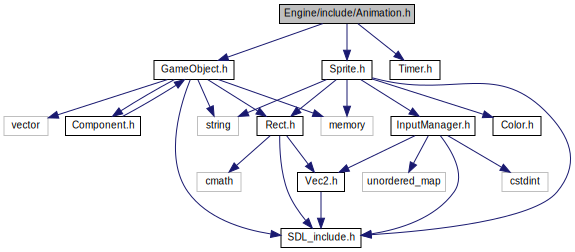
\includegraphics[width=312pt]{Animation_8h__incl}
\end{center}
\end{figure}
Este grafo mostra quais arquivos estão direta ou indiretamente relacionados com este arquivo\+:\nopagebreak
\begin{figure}[H]
\begin{center}
\leavevmode
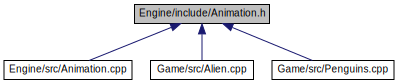
\includegraphics[width=350pt]{Animation_8h__dep__incl}
\end{center}
\end{figure}
\subsection*{Componentes}
\begin{DoxyCompactItemize}
\item 
class \hyperlink{classAnimation}{Animation}
\end{DoxyCompactItemize}

\hypertarget{Camera_8h}{\section{Referência do Arquivo Engine/include/\+Camera.h}
\label{Camera_8h}\index{Engine/include/\+Camera.\+h@{Engine/include/\+Camera.\+h}}
}
{\ttfamily \#include \char`\"{}Gameobject.\+h\char`\"{}}\\*
{\ttfamily \#include \char`\"{}Vec2.\+h\char`\"{}}\\*
Gráfico de dependência de inclusões para Camera.\+h\+:\nopagebreak
\begin{figure}[H]
\begin{center}
\leavevmode
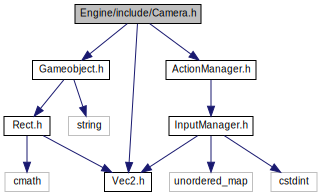
\includegraphics[width=243pt]{Camera_8h__incl}
\end{center}
\end{figure}
Este grafo mostra quais arquivos estão direta ou indiretamente relacionados com este arquivo\+:\nopagebreak
\begin{figure}[H]
\begin{center}
\leavevmode
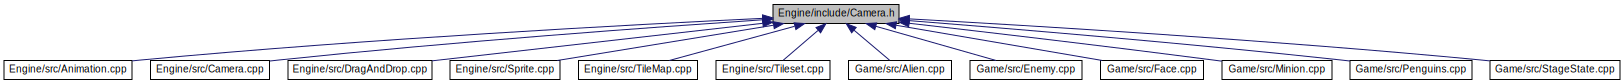
\includegraphics[width=350pt]{Camera_8h__dep__incl}
\end{center}
\end{figure}
\subsection*{Componentes}
\begin{DoxyCompactItemize}
\item 
class \hyperlink{classCamera}{Camera}
\end{DoxyCompactItemize}
\subsection*{Definições e Macros}
\begin{DoxyCompactItemize}
\item 
\#define \hyperlink{Camera_8h_a00bdac33db330ffa8021dc36c85506fe}{C\+A\+M\+E\+R\+A\+\_\+\+D\+E\+F\+A\+U\+L\+T\+\_\+\+M\+I\+N\+\_\+\+Z\+O\+O\+M}~(0.\+7)
\item 
\#define \hyperlink{Camera_8h_a53a75501f4f47ca972ec050b09df05a3}{C\+A\+M\+E\+R\+A\+\_\+\+D\+E\+F\+A\+U\+L\+T\+\_\+\+M\+A\+X\+\_\+\+Z\+O\+O\+M}~(1.\+5)
\item 
\#define \hyperlink{Camera_8h_a719f5e3a817ca056a76495044f676277}{C\+A\+M\+E\+R\+A\+\_\+\+D\+E\+F\+A\+U\+L\+T\+\_\+\+Z\+O\+O\+M\+A\+B\+L\+E}~(true)
\item 
\#define \hyperlink{Camera_8h_a896eaf751ce7e99c97bfaa76ca33f150}{C\+A\+M\+E\+R\+A\+\_\+\+D\+E\+F\+A\+U\+L\+T\+\_\+\+Z\+O\+O\+M\+\_\+\+S\+P\+E\+E\+D}~(5.\+0)
\end{DoxyCompactItemize}


\subsection{Definições e macros}
\hypertarget{Camera_8h_a53a75501f4f47ca972ec050b09df05a3}{\index{Camera.\+h@{Camera.\+h}!C\+A\+M\+E\+R\+A\+\_\+\+D\+E\+F\+A\+U\+L\+T\+\_\+\+M\+A\+X\+\_\+\+Z\+O\+O\+M@{C\+A\+M\+E\+R\+A\+\_\+\+D\+E\+F\+A\+U\+L\+T\+\_\+\+M\+A\+X\+\_\+\+Z\+O\+O\+M}}
\index{C\+A\+M\+E\+R\+A\+\_\+\+D\+E\+F\+A\+U\+L\+T\+\_\+\+M\+A\+X\+\_\+\+Z\+O\+O\+M@{C\+A\+M\+E\+R\+A\+\_\+\+D\+E\+F\+A\+U\+L\+T\+\_\+\+M\+A\+X\+\_\+\+Z\+O\+O\+M}!Camera.\+h@{Camera.\+h}}
\subsubsection[{C\+A\+M\+E\+R\+A\+\_\+\+D\+E\+F\+A\+U\+L\+T\+\_\+\+M\+A\+X\+\_\+\+Z\+O\+O\+M}]{\setlength{\rightskip}{0pt plus 5cm}\#define C\+A\+M\+E\+R\+A\+\_\+\+D\+E\+F\+A\+U\+L\+T\+\_\+\+M\+A\+X\+\_\+\+Z\+O\+O\+M~(1.\+5)}}\label{Camera_8h_a53a75501f4f47ca972ec050b09df05a3}
\hypertarget{Camera_8h_a00bdac33db330ffa8021dc36c85506fe}{\index{Camera.\+h@{Camera.\+h}!C\+A\+M\+E\+R\+A\+\_\+\+D\+E\+F\+A\+U\+L\+T\+\_\+\+M\+I\+N\+\_\+\+Z\+O\+O\+M@{C\+A\+M\+E\+R\+A\+\_\+\+D\+E\+F\+A\+U\+L\+T\+\_\+\+M\+I\+N\+\_\+\+Z\+O\+O\+M}}
\index{C\+A\+M\+E\+R\+A\+\_\+\+D\+E\+F\+A\+U\+L\+T\+\_\+\+M\+I\+N\+\_\+\+Z\+O\+O\+M@{C\+A\+M\+E\+R\+A\+\_\+\+D\+E\+F\+A\+U\+L\+T\+\_\+\+M\+I\+N\+\_\+\+Z\+O\+O\+M}!Camera.\+h@{Camera.\+h}}
\subsubsection[{C\+A\+M\+E\+R\+A\+\_\+\+D\+E\+F\+A\+U\+L\+T\+\_\+\+M\+I\+N\+\_\+\+Z\+O\+O\+M}]{\setlength{\rightskip}{0pt plus 5cm}\#define C\+A\+M\+E\+R\+A\+\_\+\+D\+E\+F\+A\+U\+L\+T\+\_\+\+M\+I\+N\+\_\+\+Z\+O\+O\+M~(0.\+7)}}\label{Camera_8h_a00bdac33db330ffa8021dc36c85506fe}
\hypertarget{Camera_8h_a896eaf751ce7e99c97bfaa76ca33f150}{\index{Camera.\+h@{Camera.\+h}!C\+A\+M\+E\+R\+A\+\_\+\+D\+E\+F\+A\+U\+L\+T\+\_\+\+Z\+O\+O\+M\+\_\+\+S\+P\+E\+E\+D@{C\+A\+M\+E\+R\+A\+\_\+\+D\+E\+F\+A\+U\+L\+T\+\_\+\+Z\+O\+O\+M\+\_\+\+S\+P\+E\+E\+D}}
\index{C\+A\+M\+E\+R\+A\+\_\+\+D\+E\+F\+A\+U\+L\+T\+\_\+\+Z\+O\+O\+M\+\_\+\+S\+P\+E\+E\+D@{C\+A\+M\+E\+R\+A\+\_\+\+D\+E\+F\+A\+U\+L\+T\+\_\+\+Z\+O\+O\+M\+\_\+\+S\+P\+E\+E\+D}!Camera.\+h@{Camera.\+h}}
\subsubsection[{C\+A\+M\+E\+R\+A\+\_\+\+D\+E\+F\+A\+U\+L\+T\+\_\+\+Z\+O\+O\+M\+\_\+\+S\+P\+E\+E\+D}]{\setlength{\rightskip}{0pt plus 5cm}\#define C\+A\+M\+E\+R\+A\+\_\+\+D\+E\+F\+A\+U\+L\+T\+\_\+\+Z\+O\+O\+M\+\_\+\+S\+P\+E\+E\+D~(5.\+0)}}\label{Camera_8h_a896eaf751ce7e99c97bfaa76ca33f150}
\hypertarget{Camera_8h_a719f5e3a817ca056a76495044f676277}{\index{Camera.\+h@{Camera.\+h}!C\+A\+M\+E\+R\+A\+\_\+\+D\+E\+F\+A\+U\+L\+T\+\_\+\+Z\+O\+O\+M\+A\+B\+L\+E@{C\+A\+M\+E\+R\+A\+\_\+\+D\+E\+F\+A\+U\+L\+T\+\_\+\+Z\+O\+O\+M\+A\+B\+L\+E}}
\index{C\+A\+M\+E\+R\+A\+\_\+\+D\+E\+F\+A\+U\+L\+T\+\_\+\+Z\+O\+O\+M\+A\+B\+L\+E@{C\+A\+M\+E\+R\+A\+\_\+\+D\+E\+F\+A\+U\+L\+T\+\_\+\+Z\+O\+O\+M\+A\+B\+L\+E}!Camera.\+h@{Camera.\+h}}
\subsubsection[{C\+A\+M\+E\+R\+A\+\_\+\+D\+E\+F\+A\+U\+L\+T\+\_\+\+Z\+O\+O\+M\+A\+B\+L\+E}]{\setlength{\rightskip}{0pt plus 5cm}\#define C\+A\+M\+E\+R\+A\+\_\+\+D\+E\+F\+A\+U\+L\+T\+\_\+\+Z\+O\+O\+M\+A\+B\+L\+E~(true)}}\label{Camera_8h_a719f5e3a817ca056a76495044f676277}

\hypertarget{Collision_8h}{\section{Referência do Arquivo Engine/include/\+Collision.h}
\label{Collision_8h}\index{Engine/include/\+Collision.\+h@{Engine/include/\+Collision.\+h}}
}
{\ttfamily \#include $<$algorithm$>$}\\*
{\ttfamily \#include \char`\"{}Rect.\+h\char`\"{}}\\*
Gráfico de dependência de inclusões para Collision.\+h\+:\nopagebreak
\begin{figure}[H]
\begin{center}
\leavevmode
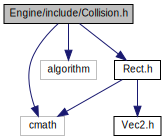
\includegraphics[width=234pt]{Collision_8h__incl}
\end{center}
\end{figure}
Este grafo mostra quais arquivos estão direta ou indiretamente relacionados com este arquivo\+:\nopagebreak
\begin{figure}[H]
\begin{center}
\leavevmode
\includegraphics[width=210pt]{Collision_8h__dep__incl}
\end{center}
\end{figure}
\subsection*{Componentes}
\begin{DoxyCompactItemize}
\item 
class \hyperlink{classCollision}{Collision}
\end{DoxyCompactItemize}

\hypertarget{Error_8h}{\section{Referência do Arquivo Engine/include/\+Error.h}
\label{Error_8h}\index{Engine/include/\+Error.\+h@{Engine/include/\+Error.\+h}}
}
{\ttfamily \#include $<$iostream$>$}\\*
{\ttfamily \#include \char`\"{}stdlib.\+h\char`\"{}}\\*
Gráfico de dependência de inclusões para Error.\+h\+:\nopagebreak
\begin{figure}[H]
\begin{center}
\leavevmode
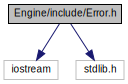
\includegraphics[width=200pt]{Error_8h__incl}
\end{center}
\end{figure}
Este grafo mostra quais arquivos estão direta ou indiretamente relacionados com este arquivo\+:\nopagebreak
\begin{figure}[H]
\begin{center}
\leavevmode
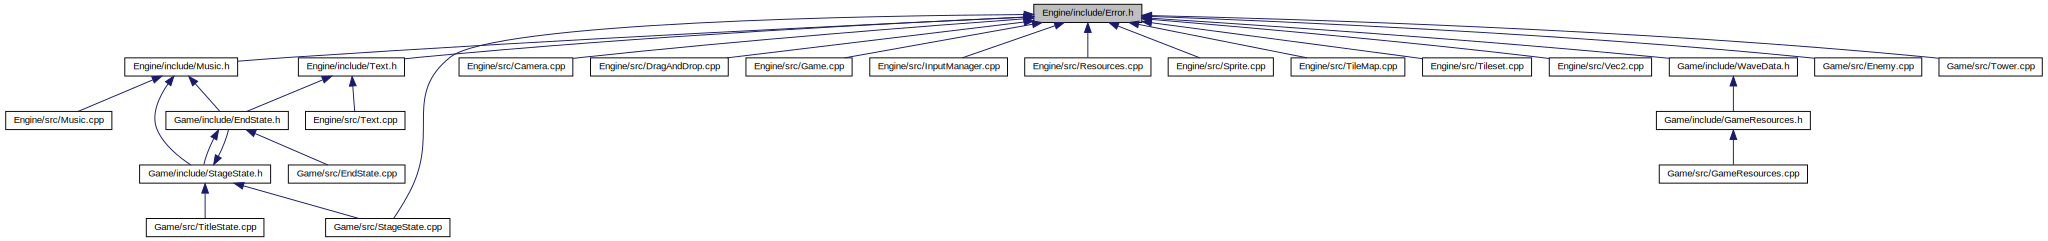
\includegraphics[width=350pt]{Error_8h__dep__incl}
\end{center}
\end{figure}
\subsection*{Definições e Macros}
\begin{DoxyCompactItemize}
\item 
\#define \hyperlink{Error_8h_a6fd2b788cc016acd19820ddb30e78c1f}{E\+N\+D\+\_\+\+L\+I\+N\+E}~\char`\"{}\textbackslash{}n\char`\"{}
\item 
\#define \hyperlink{Error_8h_ad72dbcf6d0153db1b8d8a58001feed83}{D\+E\+B\+U\+G}~0
\item 
\#define \hyperlink{Error_8h_ad7ac4f59c7725b4921af49f74536de8c}{C\+O\+N\+V\+E\+R\+S\+A\+O\+\_\+\+G\+R\+A\+U\+S\+\_\+\+R\+A\+D\+I\+A\+N\+O\+S}~57.\+324840764
\item 
\#define \hyperlink{Error_8h_a787bf097960f03921a9b9e0195d27831}{Error}(msg)~std\+::cerr$<$$<$\char`\"{}\mbox{[}E\+R\+R\+O\+R\mbox{]} \char`\"{}$<$$<$\+\_\+\+\_\+\+F\+I\+L\+E\+\_\+\+\_\+$<$$<$\char`\"{} $\vert$ \char`\"{}$<$$<$\+\_\+\+\_\+func\+\_\+\+\_\+$<$$<$\char`\"{}\+:\char`\"{}$<$$<$\+\_\+\+\_\+\+L\+I\+N\+E\+\_\+\+\_\+$<$$<$\char`\"{}\textbackslash{}t\textbackslash{}t\char`\"{}$<$$<$msg$<$$<$ \char`\"{}\textbackslash{}n\char`\"{};exit(1);
\item 
\#define \hyperlink{Error_8h_a092bd7bb2cb7fd9f483b6995cee61bc0}{A\+S\+S\+E\+R\+T}(exp)~if(!(exp))\{std\+::cerr$<$$<$\char`\"{}\mbox{[}E\+R\+R\+O\+R\mbox{]} \char`\"{}$<$$<$\+\_\+\+\_\+\+F\+I\+L\+E\+\_\+\+\_\+$<$$<$\char`\"{} $\vert$ \char`\"{}$<$$<$\+\_\+\+\_\+func\+\_\+\+\_\+$<$$<$\char`\"{}\+:\char`\"{}$<$$<$\+\_\+\+\_\+\+L\+I\+N\+E\+\_\+\+\_\+$<$$<$\char`\"{}\textbackslash{}t\textbackslash{}t\+Assertion Failed.\char`\"{}$<$$<$ \char`\"{}\textbackslash{}n\char`\"{};exit(1);\}
\item 
\#define \hyperlink{Error_8h_a5e03114cdb9780c937e89ed7cb527ae1}{S\+D\+L\+\_\+\+A\+S\+S\+E\+R\+T}(exp)~if(!(exp))\{std\+::cerr$<$$<$\char`\"{}\mbox{[}E\+R\+R\+O\+R\mbox{]} \char`\"{}$<$$<$\+\_\+\+\_\+\+F\+I\+L\+E\+\_\+\+\_\+$<$$<$\char`\"{} $\vert$ \char`\"{}$<$$<$\+\_\+\+\_\+func\+\_\+\+\_\+$<$$<$\char`\"{}\+:\char`\"{}$<$$<$\+\_\+\+\_\+\+L\+I\+N\+E\+\_\+\+\_\+$<$$<$\char`\"{}\textbackslash{}t\textbackslash{}t\+Assertion Failed\+:\char`\"{} $<$$<$ S\+D\+L\+\_\+\+Get\+Error()$<$$<$ \char`\"{}\textbackslash{}n\char`\"{};exit(1);\}
\item 
\#define \hyperlink{Error_8h_acd4a2dee55f5359c0389baab37c2f468}{W\+H\+E\+R\+E}~\+\_\+\+\_\+\+F\+I\+L\+E\+\_\+\+\_\+$<$$<$\char`\"{} $\vert$ \char`\"{}$<$$<$\+\_\+\+\_\+func\+\_\+\+\_\+$<$$<$\char`\"{}\+:\char`\"{}$<$$<$\+\_\+\+\_\+\+L\+I\+N\+E\+\_\+\+\_\+
\item 
\#define \hyperlink{Error_8h_ae8a1602ad06ce181163389d874118387}{C\+H\+E\+C\+K\+\_\+\+S\+D\+L\+\_\+\+E\+R\+R\+O\+R}~std\+::cerr$<$$<$\char`\"{}\mbox{[}E\+R\+R\+O\+R\mbox{]} \char`\"{}$<$$<$\+\_\+\+\_\+\+F\+I\+L\+E\+\_\+\+\_\+$<$$<$\char`\"{} $\vert$ \char`\"{}$<$$<$\+\_\+\+\_\+func\+\_\+\+\_\+$<$$<$\char`\"{}\+:\char`\"{}$<$$<$\+\_\+\+\_\+\+L\+I\+N\+E\+\_\+\+\_\+$<$$<$\char`\"{}\textbackslash{}t\textbackslash{}t\char`\"{}$<$$<$S\+D\+L\+\_\+\+Get\+Error()$<$$<$ \char`\"{}\textbackslash{}n\char`\"{}
\item 
\#define \hyperlink{Error_8h_a15a48a3e28c4eb425e3340eae40894c5}{R\+E\+P\+O\+R\+T\+\_\+\+I\+\_\+\+W\+A\+S\+\_\+\+H\+E\+R\+E}~if(\hyperlink{Error_8h_ad72dbcf6d0153db1b8d8a58001feed83}{D\+E\+B\+U\+G})\{std\+::cout $<$$<$\char`\"{}\mbox{[}D\+E\+B\+U\+G\mbox{]} I was here!\textbackslash{}t\char`\"{}$<$$<$\+\_\+\+\_\+\+F\+I\+L\+E\+\_\+\+\_\+$<$$<$\char`\"{} $\vert$ \char`\"{}$<$$<$\+\_\+\+\_\+func\+\_\+\+\_\+$<$$<$\char`\"{}\+:\char`\"{}$<$$<$\+\_\+\+\_\+\+L\+I\+N\+E\+\_\+\+\_\+$<$$<$\char`\"{}\textbackslash{}n\char`\"{};\}
\item 
\#define \hyperlink{Error_8h_a460a42aaa4200700dfb4a73f852e93b8}{T\+E\+M\+P\+\_\+\+R\+E\+P\+O\+R\+T\+\_\+\+I\+\_\+\+W\+A\+S\+\_\+\+H\+E\+R\+E}~if(1)\{std\+::cout $<$$<$\char`\"{}\mbox{[}D\+E\+B\+U\+G\mbox{]} I was here!\textbackslash{}t\char`\"{}$<$$<$\+\_\+\+\_\+\+F\+I\+L\+E\+\_\+\+\_\+$<$$<$\char`\"{} $\vert$ \char`\"{}$<$$<$\+\_\+\+\_\+func\+\_\+\+\_\+$<$$<$\char`\"{}\+:\char`\"{}$<$$<$\+\_\+\+\_\+\+L\+I\+N\+E\+\_\+\+\_\+$<$$<$\char`\"{}\textbackslash{}n\char`\"{};\}
\end{DoxyCompactItemize}


\subsection{Definições e macros}
\hypertarget{Error_8h_a092bd7bb2cb7fd9f483b6995cee61bc0}{\index{Error.\+h@{Error.\+h}!A\+S\+S\+E\+R\+T@{A\+S\+S\+E\+R\+T}}
\index{A\+S\+S\+E\+R\+T@{A\+S\+S\+E\+R\+T}!Error.\+h@{Error.\+h}}
\subsubsection[{A\+S\+S\+E\+R\+T}]{\setlength{\rightskip}{0pt plus 5cm}\#define A\+S\+S\+E\+R\+T(
\begin{DoxyParamCaption}
\item[{}]{exp}
\end{DoxyParamCaption}
)~if(!(exp))\{std\+::cerr$<$$<$\char`\"{}\mbox{[}E\+R\+R\+O\+R\mbox{]} \char`\"{}$<$$<$\+\_\+\+\_\+\+F\+I\+L\+E\+\_\+\+\_\+$<$$<$\char`\"{} $\vert$ \char`\"{}$<$$<$\+\_\+\+\_\+func\+\_\+\+\_\+$<$$<$\char`\"{}\+:\char`\"{}$<$$<$\+\_\+\+\_\+\+L\+I\+N\+E\+\_\+\+\_\+$<$$<$\char`\"{}\textbackslash{}t\textbackslash{}t\+Assertion Failed.\char`\"{}$<$$<$ \char`\"{}\textbackslash{}n\char`\"{};exit(1);\}}}\label{Error_8h_a092bd7bb2cb7fd9f483b6995cee61bc0}
\hypertarget{Error_8h_ae8a1602ad06ce181163389d874118387}{\index{Error.\+h@{Error.\+h}!C\+H\+E\+C\+K\+\_\+\+S\+D\+L\+\_\+\+E\+R\+R\+O\+R@{C\+H\+E\+C\+K\+\_\+\+S\+D\+L\+\_\+\+E\+R\+R\+O\+R}}
\index{C\+H\+E\+C\+K\+\_\+\+S\+D\+L\+\_\+\+E\+R\+R\+O\+R@{C\+H\+E\+C\+K\+\_\+\+S\+D\+L\+\_\+\+E\+R\+R\+O\+R}!Error.\+h@{Error.\+h}}
\subsubsection[{C\+H\+E\+C\+K\+\_\+\+S\+D\+L\+\_\+\+E\+R\+R\+O\+R}]{\setlength{\rightskip}{0pt plus 5cm}\#define C\+H\+E\+C\+K\+\_\+\+S\+D\+L\+\_\+\+E\+R\+R\+O\+R~std\+::cerr$<$$<$\char`\"{}\mbox{[}E\+R\+R\+O\+R\mbox{]} \char`\"{}$<$$<$\+\_\+\+\_\+\+F\+I\+L\+E\+\_\+\+\_\+$<$$<$\char`\"{} $\vert$ \char`\"{}$<$$<$\+\_\+\+\_\+func\+\_\+\+\_\+$<$$<$\char`\"{}\+:\char`\"{}$<$$<$\+\_\+\+\_\+\+L\+I\+N\+E\+\_\+\+\_\+$<$$<$\char`\"{}\textbackslash{}t\textbackslash{}t\char`\"{}$<$$<$S\+D\+L\+\_\+\+Get\+Error()$<$$<$ \char`\"{}\textbackslash{}n\char`\"{}}}\label{Error_8h_ae8a1602ad06ce181163389d874118387}
\hypertarget{Error_8h_ad7ac4f59c7725b4921af49f74536de8c}{\index{Error.\+h@{Error.\+h}!C\+O\+N\+V\+E\+R\+S\+A\+O\+\_\+\+G\+R\+A\+U\+S\+\_\+\+R\+A\+D\+I\+A\+N\+O\+S@{C\+O\+N\+V\+E\+R\+S\+A\+O\+\_\+\+G\+R\+A\+U\+S\+\_\+\+R\+A\+D\+I\+A\+N\+O\+S}}
\index{C\+O\+N\+V\+E\+R\+S\+A\+O\+\_\+\+G\+R\+A\+U\+S\+\_\+\+R\+A\+D\+I\+A\+N\+O\+S@{C\+O\+N\+V\+E\+R\+S\+A\+O\+\_\+\+G\+R\+A\+U\+S\+\_\+\+R\+A\+D\+I\+A\+N\+O\+S}!Error.\+h@{Error.\+h}}
\subsubsection[{C\+O\+N\+V\+E\+R\+S\+A\+O\+\_\+\+G\+R\+A\+U\+S\+\_\+\+R\+A\+D\+I\+A\+N\+O\+S}]{\setlength{\rightskip}{0pt plus 5cm}\#define C\+O\+N\+V\+E\+R\+S\+A\+O\+\_\+\+G\+R\+A\+U\+S\+\_\+\+R\+A\+D\+I\+A\+N\+O\+S~57.\+324840764}}\label{Error_8h_ad7ac4f59c7725b4921af49f74536de8c}
\hypertarget{Error_8h_ad72dbcf6d0153db1b8d8a58001feed83}{\index{Error.\+h@{Error.\+h}!D\+E\+B\+U\+G@{D\+E\+B\+U\+G}}
\index{D\+E\+B\+U\+G@{D\+E\+B\+U\+G}!Error.\+h@{Error.\+h}}
\subsubsection[{D\+E\+B\+U\+G}]{\setlength{\rightskip}{0pt plus 5cm}\#define D\+E\+B\+U\+G~0}}\label{Error_8h_ad72dbcf6d0153db1b8d8a58001feed83}
\hypertarget{Error_8h_a6fd2b788cc016acd19820ddb30e78c1f}{\index{Error.\+h@{Error.\+h}!E\+N\+D\+\_\+\+L\+I\+N\+E@{E\+N\+D\+\_\+\+L\+I\+N\+E}}
\index{E\+N\+D\+\_\+\+L\+I\+N\+E@{E\+N\+D\+\_\+\+L\+I\+N\+E}!Error.\+h@{Error.\+h}}
\subsubsection[{E\+N\+D\+\_\+\+L\+I\+N\+E}]{\setlength{\rightskip}{0pt plus 5cm}\#define E\+N\+D\+\_\+\+L\+I\+N\+E~\char`\"{}\textbackslash{}n\char`\"{}}}\label{Error_8h_a6fd2b788cc016acd19820ddb30e78c1f}
\hypertarget{Error_8h_a787bf097960f03921a9b9e0195d27831}{\index{Error.\+h@{Error.\+h}!Error@{Error}}
\index{Error@{Error}!Error.\+h@{Error.\+h}}
\subsubsection[{Error}]{\setlength{\rightskip}{0pt plus 5cm}\#define Error(
\begin{DoxyParamCaption}
\item[{}]{msg}
\end{DoxyParamCaption}
)~std\+::cerr$<$$<$\char`\"{}\mbox{[}E\+R\+R\+O\+R\mbox{]} \char`\"{}$<$$<$\+\_\+\+\_\+\+F\+I\+L\+E\+\_\+\+\_\+$<$$<$\char`\"{} $\vert$ \char`\"{}$<$$<$\+\_\+\+\_\+func\+\_\+\+\_\+$<$$<$\char`\"{}\+:\char`\"{}$<$$<$\+\_\+\+\_\+\+L\+I\+N\+E\+\_\+\+\_\+$<$$<$\char`\"{}\textbackslash{}t\textbackslash{}t\char`\"{}$<$$<$msg$<$$<$ \char`\"{}\textbackslash{}n\char`\"{};exit(1);}}\label{Error_8h_a787bf097960f03921a9b9e0195d27831}
\hypertarget{Error_8h_a15a48a3e28c4eb425e3340eae40894c5}{\index{Error.\+h@{Error.\+h}!R\+E\+P\+O\+R\+T\+\_\+\+I\+\_\+\+W\+A\+S\+\_\+\+H\+E\+R\+E@{R\+E\+P\+O\+R\+T\+\_\+\+I\+\_\+\+W\+A\+S\+\_\+\+H\+E\+R\+E}}
\index{R\+E\+P\+O\+R\+T\+\_\+\+I\+\_\+\+W\+A\+S\+\_\+\+H\+E\+R\+E@{R\+E\+P\+O\+R\+T\+\_\+\+I\+\_\+\+W\+A\+S\+\_\+\+H\+E\+R\+E}!Error.\+h@{Error.\+h}}
\subsubsection[{R\+E\+P\+O\+R\+T\+\_\+\+I\+\_\+\+W\+A\+S\+\_\+\+H\+E\+R\+E}]{\setlength{\rightskip}{0pt plus 5cm}\#define R\+E\+P\+O\+R\+T\+\_\+\+I\+\_\+\+W\+A\+S\+\_\+\+H\+E\+R\+E~if({\bf D\+E\+B\+U\+G})\{std\+::cout $<$$<$\char`\"{}\mbox{[}D\+E\+B\+U\+G\mbox{]} I was here!\textbackslash{}t\char`\"{}$<$$<$\+\_\+\+\_\+\+F\+I\+L\+E\+\_\+\+\_\+$<$$<$\char`\"{} $\vert$ \char`\"{}$<$$<$\+\_\+\+\_\+func\+\_\+\+\_\+$<$$<$\char`\"{}\+:\char`\"{}$<$$<$\+\_\+\+\_\+\+L\+I\+N\+E\+\_\+\+\_\+$<$$<$\char`\"{}\textbackslash{}n\char`\"{};\}}}\label{Error_8h_a15a48a3e28c4eb425e3340eae40894c5}
\hypertarget{Error_8h_a5e03114cdb9780c937e89ed7cb527ae1}{\index{Error.\+h@{Error.\+h}!S\+D\+L\+\_\+\+A\+S\+S\+E\+R\+T@{S\+D\+L\+\_\+\+A\+S\+S\+E\+R\+T}}
\index{S\+D\+L\+\_\+\+A\+S\+S\+E\+R\+T@{S\+D\+L\+\_\+\+A\+S\+S\+E\+R\+T}!Error.\+h@{Error.\+h}}
\subsubsection[{S\+D\+L\+\_\+\+A\+S\+S\+E\+R\+T}]{\setlength{\rightskip}{0pt plus 5cm}\#define S\+D\+L\+\_\+\+A\+S\+S\+E\+R\+T(
\begin{DoxyParamCaption}
\item[{}]{exp}
\end{DoxyParamCaption}
)~if(!(exp))\{std\+::cerr$<$$<$\char`\"{}\mbox{[}E\+R\+R\+O\+R\mbox{]} \char`\"{}$<$$<$\+\_\+\+\_\+\+F\+I\+L\+E\+\_\+\+\_\+$<$$<$\char`\"{} $\vert$ \char`\"{}$<$$<$\+\_\+\+\_\+func\+\_\+\+\_\+$<$$<$\char`\"{}\+:\char`\"{}$<$$<$\+\_\+\+\_\+\+L\+I\+N\+E\+\_\+\+\_\+$<$$<$\char`\"{}\textbackslash{}t\textbackslash{}t\+Assertion Failed\+:\char`\"{} $<$$<$ S\+D\+L\+\_\+\+Get\+Error()$<$$<$ \char`\"{}\textbackslash{}n\char`\"{};exit(1);\}}}\label{Error_8h_a5e03114cdb9780c937e89ed7cb527ae1}
\hypertarget{Error_8h_a460a42aaa4200700dfb4a73f852e93b8}{\index{Error.\+h@{Error.\+h}!T\+E\+M\+P\+\_\+\+R\+E\+P\+O\+R\+T\+\_\+\+I\+\_\+\+W\+A\+S\+\_\+\+H\+E\+R\+E@{T\+E\+M\+P\+\_\+\+R\+E\+P\+O\+R\+T\+\_\+\+I\+\_\+\+W\+A\+S\+\_\+\+H\+E\+R\+E}}
\index{T\+E\+M\+P\+\_\+\+R\+E\+P\+O\+R\+T\+\_\+\+I\+\_\+\+W\+A\+S\+\_\+\+H\+E\+R\+E@{T\+E\+M\+P\+\_\+\+R\+E\+P\+O\+R\+T\+\_\+\+I\+\_\+\+W\+A\+S\+\_\+\+H\+E\+R\+E}!Error.\+h@{Error.\+h}}
\subsubsection[{T\+E\+M\+P\+\_\+\+R\+E\+P\+O\+R\+T\+\_\+\+I\+\_\+\+W\+A\+S\+\_\+\+H\+E\+R\+E}]{\setlength{\rightskip}{0pt plus 5cm}\#define T\+E\+M\+P\+\_\+\+R\+E\+P\+O\+R\+T\+\_\+\+I\+\_\+\+W\+A\+S\+\_\+\+H\+E\+R\+E~if(1)\{std\+::cout $<$$<$\char`\"{}\mbox{[}D\+E\+B\+U\+G\mbox{]} I was here!\textbackslash{}t\char`\"{}$<$$<$\+\_\+\+\_\+\+F\+I\+L\+E\+\_\+\+\_\+$<$$<$\char`\"{} $\vert$ \char`\"{}$<$$<$\+\_\+\+\_\+func\+\_\+\+\_\+$<$$<$\char`\"{}\+:\char`\"{}$<$$<$\+\_\+\+\_\+\+L\+I\+N\+E\+\_\+\+\_\+$<$$<$\char`\"{}\textbackslash{}n\char`\"{};\}}}\label{Error_8h_a460a42aaa4200700dfb4a73f852e93b8}
\hypertarget{Error_8h_acd4a2dee55f5359c0389baab37c2f468}{\index{Error.\+h@{Error.\+h}!W\+H\+E\+R\+E@{W\+H\+E\+R\+E}}
\index{W\+H\+E\+R\+E@{W\+H\+E\+R\+E}!Error.\+h@{Error.\+h}}
\subsubsection[{W\+H\+E\+R\+E}]{\setlength{\rightskip}{0pt plus 5cm}\#define W\+H\+E\+R\+E~\+\_\+\+\_\+\+F\+I\+L\+E\+\_\+\+\_\+$<$$<$\char`\"{} $\vert$ \char`\"{}$<$$<$\+\_\+\+\_\+func\+\_\+\+\_\+$<$$<$\char`\"{}\+:\char`\"{}$<$$<$\+\_\+\+\_\+\+L\+I\+N\+E\+\_\+\+\_\+}}\label{Error_8h_acd4a2dee55f5359c0389baab37c2f468}

\hypertarget{Game_8h}{\section{Referência do Arquivo Engine/include/\+Game.h}
\label{Game_8h}\index{Engine/include/\+Game.\+h@{Engine/include/\+Game.\+h}}
}
{\ttfamily \#include $<$string$>$}\\*
{\ttfamily \#include $<$stack$>$}\\*
{\ttfamily \#include \char`\"{}State.\+h\char`\"{}}\\*
{\ttfamily \#include \char`\"{}Input\+Manager.\+h\char`\"{}}\\*
{\ttfamily \#include \char`\"{}Vec2.\+h\char`\"{}}\\*
Gráfico de dependência de inclusões para Game.\+h\+:\nopagebreak
\begin{figure}[H]
\begin{center}
\leavevmode
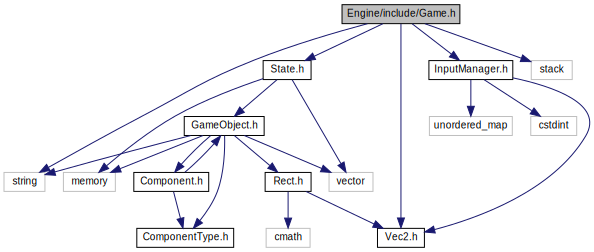
\includegraphics[width=350pt]{Game_8h__incl}
\end{center}
\end{figure}
Este grafo mostra quais arquivos estão direta ou indiretamente relacionados com este arquivo\+:\nopagebreak
\begin{figure}[H]
\begin{center}
\leavevmode
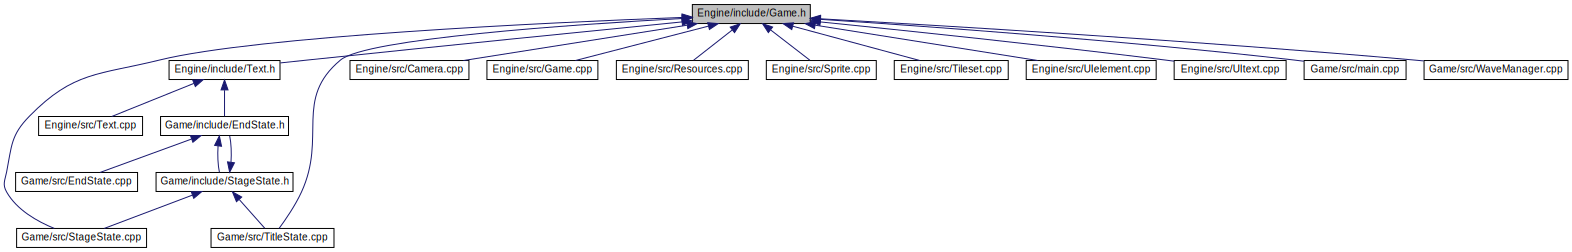
\includegraphics[width=350pt]{Game_8h__dep__incl}
\end{center}
\end{figure}
\subsection*{Componentes}
\begin{DoxyCompactItemize}
\item 
class \hyperlink{classGame}{Game}
\end{DoxyCompactItemize}
\subsection*{Definições e Macros}
\begin{DoxyCompactItemize}
\item 
\#define \hyperlink{Game_8h_aa464e7a29fa5110de8238c0cfb4458a2}{M\+I\+X\+E\+R\+\_\+\+C\+H\+U\+C\+K\+\_\+\+S\+I\+Z\+E}~1024
\end{DoxyCompactItemize}


\subsection{Definições e macros}
\hypertarget{Game_8h_aa464e7a29fa5110de8238c0cfb4458a2}{\index{Game.\+h@{Game.\+h}!M\+I\+X\+E\+R\+\_\+\+C\+H\+U\+C\+K\+\_\+\+S\+I\+Z\+E@{M\+I\+X\+E\+R\+\_\+\+C\+H\+U\+C\+K\+\_\+\+S\+I\+Z\+E}}
\index{M\+I\+X\+E\+R\+\_\+\+C\+H\+U\+C\+K\+\_\+\+S\+I\+Z\+E@{M\+I\+X\+E\+R\+\_\+\+C\+H\+U\+C\+K\+\_\+\+S\+I\+Z\+E}!Game.\+h@{Game.\+h}}
\subsubsection[{M\+I\+X\+E\+R\+\_\+\+C\+H\+U\+C\+K\+\_\+\+S\+I\+Z\+E}]{\setlength{\rightskip}{0pt plus 5cm}\#define M\+I\+X\+E\+R\+\_\+\+C\+H\+U\+C\+K\+\_\+\+S\+I\+Z\+E~1024}}\label{Game_8h_aa464e7a29fa5110de8238c0cfb4458a2}

\hypertarget{Gameobject_8h}{\section{Referência do Arquivo Engine/include/\+Gameobject.h}
\label{Gameobject_8h}\index{Engine/include/\+Gameobject.\+h@{Engine/include/\+Gameobject.\+h}}
}
{\ttfamily \#include \char`\"{}Rect.\+h\char`\"{}}\\*
{\ttfamily \#include \char`\"{}string\char`\"{}}\\*
Gráfico de dependência de inclusões para Gameobject.\+h\+:\nopagebreak
\begin{figure}[H]
\begin{center}
\leavevmode
\includegraphics[width=239pt]{Gameobject_8h__incl}
\end{center}
\end{figure}
Este grafo mostra quais arquivos estão direta ou indiretamente relacionados com este arquivo\+:\nopagebreak
\begin{figure}[H]
\begin{center}
\leavevmode
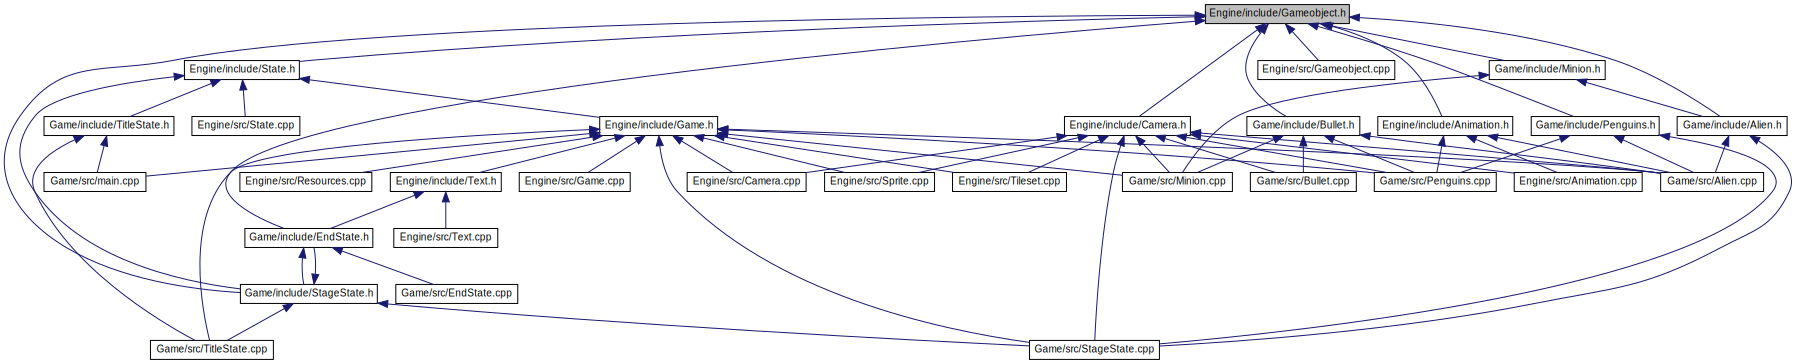
\includegraphics[width=350pt]{Gameobject_8h__dep__incl}
\end{center}
\end{figure}
\subsection*{Componentes}
\begin{DoxyCompactItemize}
\item 
class \hyperlink{classGameObject}{Game\+Object}
\end{DoxyCompactItemize}

\hypertarget{InputManager_8h}{\section{Referência do Arquivo Engine/include/\+Input\+Manager.h}
\label{InputManager_8h}\index{Engine/include/\+Input\+Manager.\+h@{Engine/include/\+Input\+Manager.\+h}}
}
{\ttfamily \#include \char`\"{}Vec2.\+h\char`\"{}}\\*
Gráfico de dependência de inclusões para Input\+Manager.\+h\+:\nopagebreak
\begin{figure}[H]
\begin{center}
\leavevmode
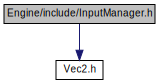
\includegraphics[width=231pt]{InputManager_8h__incl}
\end{center}
\end{figure}
Este grafo mostra quais arquivos estão direta ou indiretamente relacionados com este arquivo\+:\nopagebreak
\begin{figure}[H]
\begin{center}
\leavevmode
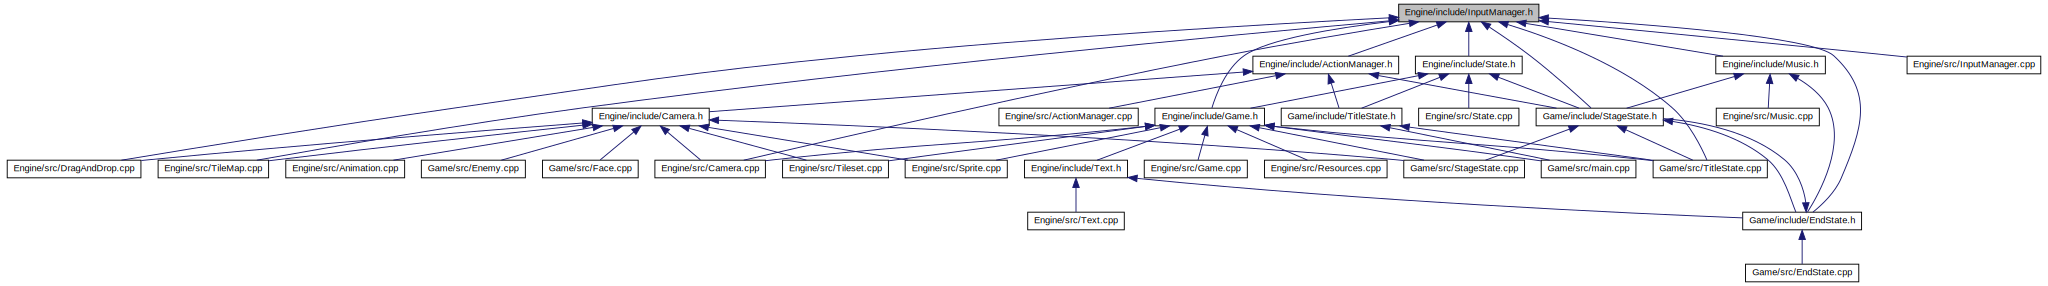
\includegraphics[width=350pt]{InputManager_8h__dep__incl}
\end{center}
\end{figure}
\subsection*{Componentes}
\begin{DoxyCompactItemize}
\item 
class \hyperlink{classInputManager}{Input\+Manager}
\end{DoxyCompactItemize}
\subsection*{Definições e Macros}
\begin{DoxyCompactItemize}
\item 
\#define \hyperlink{InputManager_8h_aea108a18c2f4dbd3bcfb53d5ec9c3e57}{L\+E\+F\+T\+\_\+\+A\+R\+R\+O\+W\+\_\+\+K\+E\+Y}~S\+D\+L\+K\+\_\+\+L\+E\+F\+T
\item 
\#define \hyperlink{InputManager_8h_ad0c8af7976bcbad226a5227851560eeb}{R\+I\+G\+H\+T\+\_\+\+A\+R\+R\+O\+W\+\_\+\+K\+E\+Y}~S\+D\+L\+K\+\_\+\+R\+I\+G\+H\+T
\item 
\#define \hyperlink{InputManager_8h_ad411242de334297d01bdadac8f47e90b}{U\+P\+\_\+\+A\+R\+R\+O\+W\+\_\+\+K\+E\+Y}~S\+D\+L\+K\+\_\+\+U\+P
\item 
\#define \hyperlink{InputManager_8h_af2292687de6b9256a2664a7dacf9ae4a}{D\+O\+W\+N\+\_\+\+A\+R\+R\+O\+W\+\_\+\+K\+E\+Y}~S\+D\+L\+K\+\_\+\+D\+O\+W\+N
\item 
\#define \hyperlink{InputManager_8h_a4c2609b38a3373c688d3888fd50808a6}{E\+S\+C\+A\+P\+E\+\_\+\+K\+E\+Y}~S\+D\+L\+K\+\_\+\+E\+S\+C\+A\+P\+E
\item 
\#define \hyperlink{InputManager_8h_a885b690ded6ea1375860b20e055d38d0}{L\+E\+F\+T\+\_\+\+A\+L\+T\+\_\+\+K\+E\+Y}~S\+D\+L\+K\+\_\+\+L\+A\+L\+T
\item 
\#define \hyperlink{InputManager_8h_ae63706b323513ebd991753c428ef13d1}{L\+E\+F\+T\+\_\+\+C\+T\+R\+L\+\_\+\+K\+E\+Y}~S\+D\+L\+K\+\_\+\+L\+C\+T\+R\+L
\item 
\#define \hyperlink{InputManager_8h_a829da24333df37749342d584fc2ba123}{L\+E\+F\+T\+\_\+\+S\+H\+I\+F\+T\+\_\+\+K\+E\+Y}~S\+D\+L\+K\+\_\+\+L\+S\+H\+I\+F\+T
\item 
\#define \hyperlink{InputManager_8h_a0d0c61d1e55887fd9a927e7f81e2deb8}{E\+S\+P\+A\+C\+E\+\_\+\+K\+E\+Y}~S\+D\+L\+K\+\_\+\+S\+P\+A\+C\+E
\item 
\#define \hyperlink{InputManager_8h_a5b4fc4bb24d4e600730ff30aaaff7323}{L\+E\+F\+T\+\_\+\+M\+O\+U\+S\+E\+\_\+\+B\+U\+T\+T\+O\+N}~S\+D\+L\+\_\+\+B\+U\+T\+T\+O\+N\+\_\+\+L\+E\+F\+T
\item 
\#define \hyperlink{InputManager_8h_a752bf1e116b4c25c5543855013c8c6eb}{R\+I\+G\+H\+T\+\_\+\+M\+O\+U\+S\+E\+\_\+\+B\+U\+T\+T\+O\+N}~S\+D\+L\+\_\+\+B\+U\+T\+T\+O\+N\+\_\+\+R\+I\+G\+H\+T
\item 
\#define \hyperlink{InputManager_8h_a0f26b1a0dee82337d947288c4ebcee16}{M\+I\+D\+D\+L\+E\+\_\+\+M\+O\+U\+S\+E\+\_\+\+B\+U\+T\+T\+O\+N}~S\+D\+L\+\_\+\+B\+U\+T\+T\+O\+N\+\_\+\+M\+I\+D\+D\+L\+E
\end{DoxyCompactItemize}


\subsection{Definições e macros}
\hypertarget{InputManager_8h_af2292687de6b9256a2664a7dacf9ae4a}{\index{Input\+Manager.\+h@{Input\+Manager.\+h}!D\+O\+W\+N\+\_\+\+A\+R\+R\+O\+W\+\_\+\+K\+E\+Y@{D\+O\+W\+N\+\_\+\+A\+R\+R\+O\+W\+\_\+\+K\+E\+Y}}
\index{D\+O\+W\+N\+\_\+\+A\+R\+R\+O\+W\+\_\+\+K\+E\+Y@{D\+O\+W\+N\+\_\+\+A\+R\+R\+O\+W\+\_\+\+K\+E\+Y}!Input\+Manager.\+h@{Input\+Manager.\+h}}
\subsubsection[{D\+O\+W\+N\+\_\+\+A\+R\+R\+O\+W\+\_\+\+K\+E\+Y}]{\setlength{\rightskip}{0pt plus 5cm}\#define D\+O\+W\+N\+\_\+\+A\+R\+R\+O\+W\+\_\+\+K\+E\+Y~S\+D\+L\+K\+\_\+\+D\+O\+W\+N}}\label{InputManager_8h_af2292687de6b9256a2664a7dacf9ae4a}
\hypertarget{InputManager_8h_a4c2609b38a3373c688d3888fd50808a6}{\index{Input\+Manager.\+h@{Input\+Manager.\+h}!E\+S\+C\+A\+P\+E\+\_\+\+K\+E\+Y@{E\+S\+C\+A\+P\+E\+\_\+\+K\+E\+Y}}
\index{E\+S\+C\+A\+P\+E\+\_\+\+K\+E\+Y@{E\+S\+C\+A\+P\+E\+\_\+\+K\+E\+Y}!Input\+Manager.\+h@{Input\+Manager.\+h}}
\subsubsection[{E\+S\+C\+A\+P\+E\+\_\+\+K\+E\+Y}]{\setlength{\rightskip}{0pt plus 5cm}\#define E\+S\+C\+A\+P\+E\+\_\+\+K\+E\+Y~S\+D\+L\+K\+\_\+\+E\+S\+C\+A\+P\+E}}\label{InputManager_8h_a4c2609b38a3373c688d3888fd50808a6}
\hypertarget{InputManager_8h_a0d0c61d1e55887fd9a927e7f81e2deb8}{\index{Input\+Manager.\+h@{Input\+Manager.\+h}!E\+S\+P\+A\+C\+E\+\_\+\+K\+E\+Y@{E\+S\+P\+A\+C\+E\+\_\+\+K\+E\+Y}}
\index{E\+S\+P\+A\+C\+E\+\_\+\+K\+E\+Y@{E\+S\+P\+A\+C\+E\+\_\+\+K\+E\+Y}!Input\+Manager.\+h@{Input\+Manager.\+h}}
\subsubsection[{E\+S\+P\+A\+C\+E\+\_\+\+K\+E\+Y}]{\setlength{\rightskip}{0pt plus 5cm}\#define E\+S\+P\+A\+C\+E\+\_\+\+K\+E\+Y~S\+D\+L\+K\+\_\+\+S\+P\+A\+C\+E}}\label{InputManager_8h_a0d0c61d1e55887fd9a927e7f81e2deb8}
\hypertarget{InputManager_8h_a885b690ded6ea1375860b20e055d38d0}{\index{Input\+Manager.\+h@{Input\+Manager.\+h}!L\+E\+F\+T\+\_\+\+A\+L\+T\+\_\+\+K\+E\+Y@{L\+E\+F\+T\+\_\+\+A\+L\+T\+\_\+\+K\+E\+Y}}
\index{L\+E\+F\+T\+\_\+\+A\+L\+T\+\_\+\+K\+E\+Y@{L\+E\+F\+T\+\_\+\+A\+L\+T\+\_\+\+K\+E\+Y}!Input\+Manager.\+h@{Input\+Manager.\+h}}
\subsubsection[{L\+E\+F\+T\+\_\+\+A\+L\+T\+\_\+\+K\+E\+Y}]{\setlength{\rightskip}{0pt plus 5cm}\#define L\+E\+F\+T\+\_\+\+A\+L\+T\+\_\+\+K\+E\+Y~S\+D\+L\+K\+\_\+\+L\+A\+L\+T}}\label{InputManager_8h_a885b690ded6ea1375860b20e055d38d0}
\hypertarget{InputManager_8h_aea108a18c2f4dbd3bcfb53d5ec9c3e57}{\index{Input\+Manager.\+h@{Input\+Manager.\+h}!L\+E\+F\+T\+\_\+\+A\+R\+R\+O\+W\+\_\+\+K\+E\+Y@{L\+E\+F\+T\+\_\+\+A\+R\+R\+O\+W\+\_\+\+K\+E\+Y}}
\index{L\+E\+F\+T\+\_\+\+A\+R\+R\+O\+W\+\_\+\+K\+E\+Y@{L\+E\+F\+T\+\_\+\+A\+R\+R\+O\+W\+\_\+\+K\+E\+Y}!Input\+Manager.\+h@{Input\+Manager.\+h}}
\subsubsection[{L\+E\+F\+T\+\_\+\+A\+R\+R\+O\+W\+\_\+\+K\+E\+Y}]{\setlength{\rightskip}{0pt plus 5cm}\#define L\+E\+F\+T\+\_\+\+A\+R\+R\+O\+W\+\_\+\+K\+E\+Y~S\+D\+L\+K\+\_\+\+L\+E\+F\+T}}\label{InputManager_8h_aea108a18c2f4dbd3bcfb53d5ec9c3e57}
\hypertarget{InputManager_8h_ae63706b323513ebd991753c428ef13d1}{\index{Input\+Manager.\+h@{Input\+Manager.\+h}!L\+E\+F\+T\+\_\+\+C\+T\+R\+L\+\_\+\+K\+E\+Y@{L\+E\+F\+T\+\_\+\+C\+T\+R\+L\+\_\+\+K\+E\+Y}}
\index{L\+E\+F\+T\+\_\+\+C\+T\+R\+L\+\_\+\+K\+E\+Y@{L\+E\+F\+T\+\_\+\+C\+T\+R\+L\+\_\+\+K\+E\+Y}!Input\+Manager.\+h@{Input\+Manager.\+h}}
\subsubsection[{L\+E\+F\+T\+\_\+\+C\+T\+R\+L\+\_\+\+K\+E\+Y}]{\setlength{\rightskip}{0pt plus 5cm}\#define L\+E\+F\+T\+\_\+\+C\+T\+R\+L\+\_\+\+K\+E\+Y~S\+D\+L\+K\+\_\+\+L\+C\+T\+R\+L}}\label{InputManager_8h_ae63706b323513ebd991753c428ef13d1}
\hypertarget{InputManager_8h_a5b4fc4bb24d4e600730ff30aaaff7323}{\index{Input\+Manager.\+h@{Input\+Manager.\+h}!L\+E\+F\+T\+\_\+\+M\+O\+U\+S\+E\+\_\+\+B\+U\+T\+T\+O\+N@{L\+E\+F\+T\+\_\+\+M\+O\+U\+S\+E\+\_\+\+B\+U\+T\+T\+O\+N}}
\index{L\+E\+F\+T\+\_\+\+M\+O\+U\+S\+E\+\_\+\+B\+U\+T\+T\+O\+N@{L\+E\+F\+T\+\_\+\+M\+O\+U\+S\+E\+\_\+\+B\+U\+T\+T\+O\+N}!Input\+Manager.\+h@{Input\+Manager.\+h}}
\subsubsection[{L\+E\+F\+T\+\_\+\+M\+O\+U\+S\+E\+\_\+\+B\+U\+T\+T\+O\+N}]{\setlength{\rightskip}{0pt plus 5cm}\#define L\+E\+F\+T\+\_\+\+M\+O\+U\+S\+E\+\_\+\+B\+U\+T\+T\+O\+N~S\+D\+L\+\_\+\+B\+U\+T\+T\+O\+N\+\_\+\+L\+E\+F\+T}}\label{InputManager_8h_a5b4fc4bb24d4e600730ff30aaaff7323}
\hypertarget{InputManager_8h_a829da24333df37749342d584fc2ba123}{\index{Input\+Manager.\+h@{Input\+Manager.\+h}!L\+E\+F\+T\+\_\+\+S\+H\+I\+F\+T\+\_\+\+K\+E\+Y@{L\+E\+F\+T\+\_\+\+S\+H\+I\+F\+T\+\_\+\+K\+E\+Y}}
\index{L\+E\+F\+T\+\_\+\+S\+H\+I\+F\+T\+\_\+\+K\+E\+Y@{L\+E\+F\+T\+\_\+\+S\+H\+I\+F\+T\+\_\+\+K\+E\+Y}!Input\+Manager.\+h@{Input\+Manager.\+h}}
\subsubsection[{L\+E\+F\+T\+\_\+\+S\+H\+I\+F\+T\+\_\+\+K\+E\+Y}]{\setlength{\rightskip}{0pt plus 5cm}\#define L\+E\+F\+T\+\_\+\+S\+H\+I\+F\+T\+\_\+\+K\+E\+Y~S\+D\+L\+K\+\_\+\+L\+S\+H\+I\+F\+T}}\label{InputManager_8h_a829da24333df37749342d584fc2ba123}
\hypertarget{InputManager_8h_a0f26b1a0dee82337d947288c4ebcee16}{\index{Input\+Manager.\+h@{Input\+Manager.\+h}!M\+I\+D\+D\+L\+E\+\_\+\+M\+O\+U\+S\+E\+\_\+\+B\+U\+T\+T\+O\+N@{M\+I\+D\+D\+L\+E\+\_\+\+M\+O\+U\+S\+E\+\_\+\+B\+U\+T\+T\+O\+N}}
\index{M\+I\+D\+D\+L\+E\+\_\+\+M\+O\+U\+S\+E\+\_\+\+B\+U\+T\+T\+O\+N@{M\+I\+D\+D\+L\+E\+\_\+\+M\+O\+U\+S\+E\+\_\+\+B\+U\+T\+T\+O\+N}!Input\+Manager.\+h@{Input\+Manager.\+h}}
\subsubsection[{M\+I\+D\+D\+L\+E\+\_\+\+M\+O\+U\+S\+E\+\_\+\+B\+U\+T\+T\+O\+N}]{\setlength{\rightskip}{0pt plus 5cm}\#define M\+I\+D\+D\+L\+E\+\_\+\+M\+O\+U\+S\+E\+\_\+\+B\+U\+T\+T\+O\+N~S\+D\+L\+\_\+\+B\+U\+T\+T\+O\+N\+\_\+\+M\+I\+D\+D\+L\+E}}\label{InputManager_8h_a0f26b1a0dee82337d947288c4ebcee16}
\hypertarget{InputManager_8h_ad0c8af7976bcbad226a5227851560eeb}{\index{Input\+Manager.\+h@{Input\+Manager.\+h}!R\+I\+G\+H\+T\+\_\+\+A\+R\+R\+O\+W\+\_\+\+K\+E\+Y@{R\+I\+G\+H\+T\+\_\+\+A\+R\+R\+O\+W\+\_\+\+K\+E\+Y}}
\index{R\+I\+G\+H\+T\+\_\+\+A\+R\+R\+O\+W\+\_\+\+K\+E\+Y@{R\+I\+G\+H\+T\+\_\+\+A\+R\+R\+O\+W\+\_\+\+K\+E\+Y}!Input\+Manager.\+h@{Input\+Manager.\+h}}
\subsubsection[{R\+I\+G\+H\+T\+\_\+\+A\+R\+R\+O\+W\+\_\+\+K\+E\+Y}]{\setlength{\rightskip}{0pt plus 5cm}\#define R\+I\+G\+H\+T\+\_\+\+A\+R\+R\+O\+W\+\_\+\+K\+E\+Y~S\+D\+L\+K\+\_\+\+R\+I\+G\+H\+T}}\label{InputManager_8h_ad0c8af7976bcbad226a5227851560eeb}
\hypertarget{InputManager_8h_a752bf1e116b4c25c5543855013c8c6eb}{\index{Input\+Manager.\+h@{Input\+Manager.\+h}!R\+I\+G\+H\+T\+\_\+\+M\+O\+U\+S\+E\+\_\+\+B\+U\+T\+T\+O\+N@{R\+I\+G\+H\+T\+\_\+\+M\+O\+U\+S\+E\+\_\+\+B\+U\+T\+T\+O\+N}}
\index{R\+I\+G\+H\+T\+\_\+\+M\+O\+U\+S\+E\+\_\+\+B\+U\+T\+T\+O\+N@{R\+I\+G\+H\+T\+\_\+\+M\+O\+U\+S\+E\+\_\+\+B\+U\+T\+T\+O\+N}!Input\+Manager.\+h@{Input\+Manager.\+h}}
\subsubsection[{R\+I\+G\+H\+T\+\_\+\+M\+O\+U\+S\+E\+\_\+\+B\+U\+T\+T\+O\+N}]{\setlength{\rightskip}{0pt plus 5cm}\#define R\+I\+G\+H\+T\+\_\+\+M\+O\+U\+S\+E\+\_\+\+B\+U\+T\+T\+O\+N~S\+D\+L\+\_\+\+B\+U\+T\+T\+O\+N\+\_\+\+R\+I\+G\+H\+T}}\label{InputManager_8h_a752bf1e116b4c25c5543855013c8c6eb}
\hypertarget{InputManager_8h_ad411242de334297d01bdadac8f47e90b}{\index{Input\+Manager.\+h@{Input\+Manager.\+h}!U\+P\+\_\+\+A\+R\+R\+O\+W\+\_\+\+K\+E\+Y@{U\+P\+\_\+\+A\+R\+R\+O\+W\+\_\+\+K\+E\+Y}}
\index{U\+P\+\_\+\+A\+R\+R\+O\+W\+\_\+\+K\+E\+Y@{U\+P\+\_\+\+A\+R\+R\+O\+W\+\_\+\+K\+E\+Y}!Input\+Manager.\+h@{Input\+Manager.\+h}}
\subsubsection[{U\+P\+\_\+\+A\+R\+R\+O\+W\+\_\+\+K\+E\+Y}]{\setlength{\rightskip}{0pt plus 5cm}\#define U\+P\+\_\+\+A\+R\+R\+O\+W\+\_\+\+K\+E\+Y~S\+D\+L\+K\+\_\+\+U\+P}}\label{InputManager_8h_ad411242de334297d01bdadac8f47e90b}

\hypertarget{Music_8h}{\section{Referência do Arquivo Engine/include/\+Music.h}
\label{Music_8h}\index{Engine/include/\+Music.\+h@{Engine/include/\+Music.\+h}}
}
{\ttfamily \#include $<$string$>$}\\*
{\ttfamily \#include \char`\"{}Resources.\+h\char`\"{}}\\*
{\ttfamily \#include \char`\"{}Error.\+h\char`\"{}}\\*
Gráfico de dependência de inclusões para Music.\+h\+:\nopagebreak
\begin{figure}[H]
\begin{center}
\leavevmode
\includegraphics[width=350pt]{Music_8h__incl}
\end{center}
\end{figure}
Este grafo mostra quais arquivos estão direta ou indiretamente relacionados com este arquivo\+:\nopagebreak
\begin{figure}[H]
\begin{center}
\leavevmode
\includegraphics[width=350pt]{Music_8h__dep__incl}
\end{center}
\end{figure}
\subsection*{Componentes}
\begin{DoxyCompactItemize}
\item 
class \hyperlink{classMusic}{Music}
\end{DoxyCompactItemize}
\subsection*{Definições e Macros}
\begin{DoxyCompactItemize}
\item 
\#define \hyperlink{Music_8h_a56d75cf0fabf795cc2ec85cdfa487bf2}{M\+U\+S\+I\+C\+\_\+\+F\+A\+D\+E\+\_\+\+O\+U\+T\+\_\+\+T\+I\+M\+E\+\_\+\+M\+S\+E\+C}~(2000)
\end{DoxyCompactItemize}


\subsection{Definições e macros}
\hypertarget{Music_8h_a56d75cf0fabf795cc2ec85cdfa487bf2}{\index{Music.\+h@{Music.\+h}!M\+U\+S\+I\+C\+\_\+\+F\+A\+D\+E\+\_\+\+O\+U\+T\+\_\+\+T\+I\+M\+E\+\_\+\+M\+S\+E\+C@{M\+U\+S\+I\+C\+\_\+\+F\+A\+D\+E\+\_\+\+O\+U\+T\+\_\+\+T\+I\+M\+E\+\_\+\+M\+S\+E\+C}}
\index{M\+U\+S\+I\+C\+\_\+\+F\+A\+D\+E\+\_\+\+O\+U\+T\+\_\+\+T\+I\+M\+E\+\_\+\+M\+S\+E\+C@{M\+U\+S\+I\+C\+\_\+\+F\+A\+D\+E\+\_\+\+O\+U\+T\+\_\+\+T\+I\+M\+E\+\_\+\+M\+S\+E\+C}!Music.\+h@{Music.\+h}}
\subsubsection[{M\+U\+S\+I\+C\+\_\+\+F\+A\+D\+E\+\_\+\+O\+U\+T\+\_\+\+T\+I\+M\+E\+\_\+\+M\+S\+E\+C}]{\setlength{\rightskip}{0pt plus 5cm}\#define M\+U\+S\+I\+C\+\_\+\+F\+A\+D\+E\+\_\+\+O\+U\+T\+\_\+\+T\+I\+M\+E\+\_\+\+M\+S\+E\+C~(2000)}}\label{Music_8h_a56d75cf0fabf795cc2ec85cdfa487bf2}

\hypertarget{Rect_8h}{\section{Referência do Arquivo Engine/include/\+Rect.h}
\label{Rect_8h}\index{Engine/include/\+Rect.\+h@{Engine/include/\+Rect.\+h}}
}
{\ttfamily \#include \char`\"{}Vec2.\+h\char`\"{}}\\*
{\ttfamily \#include $<$cmath$>$}\\*
Gráfico de dependência de inclusões para Rect.\+h\+:\nopagebreak
\begin{figure}[H]
\begin{center}
\leavevmode
\includegraphics[width=193pt]{Rect_8h__incl}
\end{center}
\end{figure}
Este grafo mostra quais arquivos estão direta ou indiretamente relacionados com este arquivo\+:\nopagebreak
\begin{figure}[H]
\begin{center}
\leavevmode
\includegraphics[width=350pt]{Rect_8h__dep__incl}
\end{center}
\end{figure}
\subsection*{Componentes}
\begin{DoxyCompactItemize}
\item 
class \hyperlink{classRect}{Rect}
\end{DoxyCompactItemize}

\hypertarget{Resources_8h}{\section{Referência do Arquivo Engine/include/\+Resources.h}
\label{Resources_8h}\index{Engine/include/\+Resources.\+h@{Engine/include/\+Resources.\+h}}
}
{\ttfamily \#include $<$string$>$}\\*
{\ttfamily \#include $<$unordered\+\_\+map$>$}\\*
{\ttfamily \#include $<$memory$>$}\\*
Gráfico de dependência de inclusões para Resources.\+h\+:\nopagebreak
\begin{figure}[H]
\begin{center}
\leavevmode
\includegraphics[width=293pt]{Resources_8h__incl}
\end{center}
\end{figure}
Este grafo mostra quais arquivos estão direta ou indiretamente relacionados com este arquivo\+:\nopagebreak
\begin{figure}[H]
\begin{center}
\leavevmode
\includegraphics[width=350pt]{Resources_8h__dep__incl}
\end{center}
\end{figure}
\subsection*{Componentes}
\begin{DoxyCompactItemize}
\item 
class \hyperlink{classResources}{Resources}
\end{DoxyCompactItemize}

\hypertarget{Sound_8h}{\section{Referência do Arquivo Engine/include/\+Sound.h}
\label{Sound_8h}\index{Engine/include/\+Sound.\+h@{Engine/include/\+Sound.\+h}}
}
{\ttfamily \#include $<$memory$>$}\\*
{\ttfamily \#include $<$string$>$}\\*
Gráfico de dependência de inclusões para Sound.\+h\+:\nopagebreak
\begin{figure}[H]
\begin{center}
\leavevmode
\includegraphics[width=199pt]{Sound_8h__incl}
\end{center}
\end{figure}
Este grafo mostra quais arquivos estão direta ou indiretamente relacionados com este arquivo\+:\nopagebreak
\begin{figure}[H]
\begin{center}
\leavevmode
\includegraphics[width=350pt]{Sound_8h__dep__incl}
\end{center}
\end{figure}
\subsection*{Componentes}
\begin{DoxyCompactItemize}
\item 
class \hyperlink{classSound}{Sound}
\end{DoxyCompactItemize}

\hypertarget{Sprite_8h}{\section{Referência do Arquivo Engine/include/\+Sprite.h}
\label{Sprite_8h}\index{Engine/include/\+Sprite.\+h@{Engine/include/\+Sprite.\+h}}
}
{\ttfamily \#include $<$string$>$}\\*
{\ttfamily \#include $<$memory$>$}\\*
Gráfico de dependência de inclusões para Sprite.\+h\+:\nopagebreak
\begin{figure}[H]
\begin{center}
\leavevmode
\includegraphics[width=198pt]{Sprite_8h__incl}
\end{center}
\end{figure}
Este grafo mostra quais arquivos estão direta ou indiretamente relacionados com este arquivo\+:\nopagebreak
\begin{figure}[H]
\begin{center}
\leavevmode
\includegraphics[width=350pt]{Sprite_8h__dep__incl}
\end{center}
\end{figure}
\subsection*{Componentes}
\begin{DoxyCompactItemize}
\item 
class \hyperlink{classSprite}{Sprite}
\end{DoxyCompactItemize}

\hypertarget{State_8h}{\section{Referência do Arquivo Engine/include/\+State.h}
\label{State_8h}\index{Engine/include/\+State.\+h@{Engine/include/\+State.\+h}}
}
{\ttfamily \#include \char`\"{}Gameobject.\+h\char`\"{}}\\*
{\ttfamily \#include $<$vector$>$}\\*
{\ttfamily \#include $<$memory$>$}\\*
Gráfico de dependência de inclusões para State.\+h\+:\nopagebreak
\begin{figure}[H]
\begin{center}
\leavevmode
\includegraphics[width=338pt]{State_8h__incl}
\end{center}
\end{figure}
Este grafo mostra quais arquivos estão direta ou indiretamente relacionados com este arquivo\+:\nopagebreak
\begin{figure}[H]
\begin{center}
\leavevmode
\includegraphics[width=350pt]{State_8h__dep__incl}
\end{center}
\end{figure}
\subsection*{Componentes}
\begin{DoxyCompactItemize}
\item 
class \hyperlink{classState}{State}
\end{DoxyCompactItemize}

\hypertarget{StateData_8h}{\section{Referência do Arquivo Engine/include/\+State\+Data.h}
\label{StateData_8h}\index{Engine/include/\+State\+Data.\+h@{Engine/include/\+State\+Data.\+h}}
}
Este grafo mostra quais arquivos estão direta ou indiretamente relacionados com este arquivo\+:\nopagebreak
\begin{figure}[H]
\begin{center}
\leavevmode
\includegraphics[width=350pt]{StateData_8h__dep__incl}
\end{center}
\end{figure}
\subsection*{Componentes}
\begin{DoxyCompactItemize}
\item 
class \hyperlink{classStateData}{State\+Data}
\end{DoxyCompactItemize}
\subsection*{Definições de Tipos}
\begin{DoxyCompactItemize}
\item 
typedef int \hyperlink{StateData_8h_a11e85d0fc3db733c13a8d9d030471c7d}{State\+Data\+Type}
\end{DoxyCompactItemize}


\subsection{Definições dos tipos}
\hypertarget{StateData_8h_a11e85d0fc3db733c13a8d9d030471c7d}{\index{State\+Data.\+h@{State\+Data.\+h}!State\+Data\+Type@{State\+Data\+Type}}
\index{State\+Data\+Type@{State\+Data\+Type}!State\+Data.\+h@{State\+Data.\+h}}
\subsubsection[{State\+Data\+Type}]{\setlength{\rightskip}{0pt plus 5cm}typedef int {\bf State\+Data\+Type}}}\label{StateData_8h_a11e85d0fc3db733c13a8d9d030471c7d}

\hypertarget{Text_8h}{\section{Referência do Arquivo Engine/include/\+Text.h}
\label{Text_8h}\index{Engine/include/\+Text.\+h@{Engine/include/\+Text.\+h}}
}
{\ttfamily \#include \char`\"{}Rect.\+h\char`\"{}}\\*
{\ttfamily \#include $<$memory$>$}\\*
{\ttfamily \#include $<$string$>$}\\*
{\ttfamily \#include \char`\"{}Resources.\+h\char`\"{}}\\*
{\ttfamily \#include \char`\"{}Game.\+h\char`\"{}}\\*
{\ttfamily \#include \char`\"{}Error.\+h\char`\"{}}\\*
Gráfico de dependência de inclusões para Text.\+h\+:\nopagebreak
\begin{figure}[H]
\begin{center}
\leavevmode
\includegraphics[width=350pt]{Text_8h__incl}
\end{center}
\end{figure}
Este grafo mostra quais arquivos estão direta ou indiretamente relacionados com este arquivo\+:\nopagebreak
\begin{figure}[H]
\begin{center}
\leavevmode
\includegraphics[width=350pt]{Text_8h__dep__incl}
\end{center}
\end{figure}
\subsection*{Componentes}
\begin{DoxyCompactItemize}
\item 
class \hyperlink{classText}{Text}
\end{DoxyCompactItemize}
\subsection*{Enumerações}
\begin{DoxyCompactItemize}
\item 
enum \hyperlink{Text_8h_ad5957a553b7d89d4921c39cc3ad6bc45}{Text\+Style} \{ \hyperlink{Text_8h_ad5957a553b7d89d4921c39cc3ad6bc45a1b45f84e1f6603b52e5ef442836df9af}{S\+O\+L\+I\+D}, 
\hyperlink{Text_8h_ad5957a553b7d89d4921c39cc3ad6bc45a9c46e16a4ab019339596acadeefc8c53}{S\+H\+A\+R\+E\+D}, 
\hyperlink{Text_8h_ad5957a553b7d89d4921c39cc3ad6bc45a2dddf3d92f4ebca37b63bfd88f337f3a}{B\+L\+E\+N\+D\+E\+D}
 \}
\end{DoxyCompactItemize}


\subsection{Enumerações}
\hypertarget{Text_8h_ad5957a553b7d89d4921c39cc3ad6bc45}{\index{Text.\+h@{Text.\+h}!Text\+Style@{Text\+Style}}
\index{Text\+Style@{Text\+Style}!Text.\+h@{Text.\+h}}
\subsubsection[{Text\+Style}]{\setlength{\rightskip}{0pt plus 5cm}enum {\bf Text\+Style}}}\label{Text_8h_ad5957a553b7d89d4921c39cc3ad6bc45}
\begin{Desc}
\item[Valores enumerados]\par
\begin{description}
\index{S\+O\+L\+I\+D@{S\+O\+L\+I\+D}!Text.\+h@{Text.\+h}}\index{Text.\+h@{Text.\+h}!S\+O\+L\+I\+D@{S\+O\+L\+I\+D}}\item[{\em 
\hypertarget{Text_8h_ad5957a553b7d89d4921c39cc3ad6bc45a1b45f84e1f6603b52e5ef442836df9af}{S\+O\+L\+I\+D}\label{Text_8h_ad5957a553b7d89d4921c39cc3ad6bc45a1b45f84e1f6603b52e5ef442836df9af}
}]\index{S\+H\+A\+R\+E\+D@{S\+H\+A\+R\+E\+D}!Text.\+h@{Text.\+h}}\index{Text.\+h@{Text.\+h}!S\+H\+A\+R\+E\+D@{S\+H\+A\+R\+E\+D}}\item[{\em 
\hypertarget{Text_8h_ad5957a553b7d89d4921c39cc3ad6bc45a9c46e16a4ab019339596acadeefc8c53}{S\+H\+A\+R\+E\+D}\label{Text_8h_ad5957a553b7d89d4921c39cc3ad6bc45a9c46e16a4ab019339596acadeefc8c53}
}]\index{B\+L\+E\+N\+D\+E\+D@{B\+L\+E\+N\+D\+E\+D}!Text.\+h@{Text.\+h}}\index{Text.\+h@{Text.\+h}!B\+L\+E\+N\+D\+E\+D@{B\+L\+E\+N\+D\+E\+D}}\item[{\em 
\hypertarget{Text_8h_ad5957a553b7d89d4921c39cc3ad6bc45a2dddf3d92f4ebca37b63bfd88f337f3a}{B\+L\+E\+N\+D\+E\+D}\label{Text_8h_ad5957a553b7d89d4921c39cc3ad6bc45a2dddf3d92f4ebca37b63bfd88f337f3a}
}]\end{description}
\end{Desc}

\hypertarget{TileMap_8h}{\section{Referência do Arquivo Engine/include/\+Tile\+Map.h}
\label{TileMap_8h}\index{Engine/include/\+Tile\+Map.\+h@{Engine/include/\+Tile\+Map.\+h}}
}
{\ttfamily \#include $<$string$>$}\\*
{\ttfamily \#include $<$vector$>$}\\*
{\ttfamily \#include \char`\"{}Tileset.\+h\char`\"{}}\\*
Gráfico de dependência de inclusões para Tile\+Map.\+h\+:\nopagebreak
\begin{figure}[H]
\begin{center}
\leavevmode
\includegraphics[width=242pt]{TileMap_8h__incl}
\end{center}
\end{figure}
Este grafo mostra quais arquivos estão direta ou indiretamente relacionados com este arquivo\+:\nopagebreak
\begin{figure}[H]
\begin{center}
\leavevmode
\includegraphics[width=350pt]{TileMap_8h__dep__incl}
\end{center}
\end{figure}
\subsection*{Componentes}
\begin{DoxyCompactItemize}
\item 
class \hyperlink{classTileMap}{Tile\+Map}
\end{DoxyCompactItemize}
\subsection*{Definições e Macros}
\begin{DoxyCompactItemize}
\item 
\#define \hyperlink{TileMap_8h_ac02aac1b0a1bc1430a2bf4a3cd4ab7bf}{T\+I\+L\+E\+\_\+\+V\+A\+Z\+I\+O}~-\/1
\end{DoxyCompactItemize}


\subsection{Definições e macros}
\hypertarget{TileMap_8h_ac02aac1b0a1bc1430a2bf4a3cd4ab7bf}{\index{Tile\+Map.\+h@{Tile\+Map.\+h}!T\+I\+L\+E\+\_\+\+V\+A\+Z\+I\+O@{T\+I\+L\+E\+\_\+\+V\+A\+Z\+I\+O}}
\index{T\+I\+L\+E\+\_\+\+V\+A\+Z\+I\+O@{T\+I\+L\+E\+\_\+\+V\+A\+Z\+I\+O}!Tile\+Map.\+h@{Tile\+Map.\+h}}
\subsubsection[{T\+I\+L\+E\+\_\+\+V\+A\+Z\+I\+O}]{\setlength{\rightskip}{0pt plus 5cm}\#define T\+I\+L\+E\+\_\+\+V\+A\+Z\+I\+O~-\/1}}\label{TileMap_8h_ac02aac1b0a1bc1430a2bf4a3cd4ab7bf}

\hypertarget{Tileset_8h}{\section{Referência do Arquivo Engine/include/\+Tileset.h}
\label{Tileset_8h}\index{Engine/include/\+Tileset.\+h@{Engine/include/\+Tileset.\+h}}
}
{\ttfamily \#include $<$string$>$}\\*
{\ttfamily \#include \char`\"{}Sprite.\+h\char`\"{}}\\*
Gráfico de dependência de inclusões para Tileset.\+h\+:\nopagebreak
\begin{figure}[H]
\begin{center}
\leavevmode
\includegraphics[width=206pt]{Tileset_8h__incl}
\end{center}
\end{figure}
Este grafo mostra quais arquivos estão direta ou indiretamente relacionados com este arquivo\+:\nopagebreak
\begin{figure}[H]
\begin{center}
\leavevmode
\includegraphics[width=350pt]{Tileset_8h__dep__incl}
\end{center}
\end{figure}
\subsection*{Componentes}
\begin{DoxyCompactItemize}
\item 
class \hyperlink{classTileSet}{Tile\+Set}
\end{DoxyCompactItemize}

\hypertarget{Timer_8h}{\section{Referência do Arquivo Engine/include/\+Timer.h}
\label{Timer_8h}\index{Engine/include/\+Timer.\+h@{Engine/include/\+Timer.\+h}}
}
Este grafo mostra quais arquivos estão direta ou indiretamente relacionados com este arquivo\+:\nopagebreak
\begin{figure}[H]
\begin{center}
\leavevmode
\includegraphics[width=350pt]{Timer_8h__dep__incl}
\end{center}
\end{figure}
\subsection*{Componentes}
\begin{DoxyCompactItemize}
\item 
class \hyperlink{classTimer}{Timer}
\end{DoxyCompactItemize}

\hypertarget{Vec2_8h}{\section{Referência do Arquivo Engine/include/\+Vec2.h}
\label{Vec2_8h}\index{Engine/include/\+Vec2.\+h@{Engine/include/\+Vec2.\+h}}
}
Este grafo mostra quais arquivos estão direta ou indiretamente relacionados com este arquivo\+:\nopagebreak
\begin{figure}[H]
\begin{center}
\leavevmode
\includegraphics[width=350pt]{Vec2_8h__dep__incl}
\end{center}
\end{figure}
\subsection*{Componentes}
\begin{DoxyCompactItemize}
\item 
class \hyperlink{classVec2}{Vec2}
\end{DoxyCompactItemize}
\subsection*{Definições e Macros}
\begin{DoxyCompactItemize}
\item 
\#define \hyperlink{Vec2_8h_a1759b83db156ac7ed195b3e04757ee14}{M\+A\+R\+G\+E\+M\+\_\+\+E\+R\+R\+O\+\_\+\+C\+O\+M\+P\+A\+R\+A\+C\+A\+O}~(0.\+1)
\end{DoxyCompactItemize}


\subsection{Definições e macros}
\hypertarget{Vec2_8h_a1759b83db156ac7ed195b3e04757ee14}{\index{Vec2.\+h@{Vec2.\+h}!M\+A\+R\+G\+E\+M\+\_\+\+E\+R\+R\+O\+\_\+\+C\+O\+M\+P\+A\+R\+A\+C\+A\+O@{M\+A\+R\+G\+E\+M\+\_\+\+E\+R\+R\+O\+\_\+\+C\+O\+M\+P\+A\+R\+A\+C\+A\+O}}
\index{M\+A\+R\+G\+E\+M\+\_\+\+E\+R\+R\+O\+\_\+\+C\+O\+M\+P\+A\+R\+A\+C\+A\+O@{M\+A\+R\+G\+E\+M\+\_\+\+E\+R\+R\+O\+\_\+\+C\+O\+M\+P\+A\+R\+A\+C\+A\+O}!Vec2.\+h@{Vec2.\+h}}
\subsubsection[{M\+A\+R\+G\+E\+M\+\_\+\+E\+R\+R\+O\+\_\+\+C\+O\+M\+P\+A\+R\+A\+C\+A\+O}]{\setlength{\rightskip}{0pt plus 5cm}\#define M\+A\+R\+G\+E\+M\+\_\+\+E\+R\+R\+O\+\_\+\+C\+O\+M\+P\+A\+R\+A\+C\+A\+O~(0.\+1)}}\label{Vec2_8h_a1759b83db156ac7ed195b3e04757ee14}

\hypertarget{Animation_8cpp}{\section{Referência do Arquivo Engine/src/\+Animation.cpp}
\label{Animation_8cpp}\index{Engine/src/\+Animation.\+cpp@{Engine/src/\+Animation.\+cpp}}
}
{\ttfamily \#include \char`\"{}Animation.\+h\char`\"{}}\\*
{\ttfamily \#include \char`\"{}Camera.\+h\char`\"{}}\\*
Gráfico de dependência de inclusões para Animation.\+cpp\+:\nopagebreak
\begin{figure}[H]
\begin{center}
\leavevmode
\includegraphics[width=346pt]{Animation_8cpp__incl}
\end{center}
\end{figure}

\hypertarget{Camera_8cpp}{\section{Referência do Arquivo Engine/src/\+Camera.cpp}
\label{Camera_8cpp}\index{Engine/src/\+Camera.\+cpp@{Engine/src/\+Camera.\+cpp}}
}
{\ttfamily \#include \char`\"{}Camera.\+h\char`\"{}}\\*
{\ttfamily \#include \char`\"{}Input\+Manager.\+h\char`\"{}}\\*
{\ttfamily \#include \char`\"{}Error.\+h\char`\"{}}\\*
{\ttfamily \#include \char`\"{}Game.\+h\char`\"{}}\\*
Gráfico de dependência de inclusões para Camera.\+cpp\+:\nopagebreak
\begin{figure}[H]
\begin{center}
\leavevmode
\includegraphics[width=350pt]{Camera_8cpp__incl}
\end{center}
\end{figure}
\subsection*{Definições e Macros}
\begin{DoxyCompactItemize}
\item 
\#define \hyperlink{Camera_8cpp_a6962606bd42615342e6dc4ab58ad5cd4}{C\+A\+M\+E\+R\+A\+\_\+\+M\+O\+V\+E\+\_\+\+S\+P\+E\+E\+D}~(100)
\item 
\#define \hyperlink{Camera_8cpp_ad2c7741149bf2d26ce3649737749d3ff}{I\+N\+P\+U\+T\+\_\+\+M\+A\+N\+A\+G\+E\+R}~\hyperlink{classInputManager_a1f095ed502f0bd09390d05cdc0acdcd9}{Input\+Manager\+::\+Get\+Instance}()
\end{DoxyCompactItemize}


\subsection{Definições e macros}
\hypertarget{Camera_8cpp_a6962606bd42615342e6dc4ab58ad5cd4}{\index{Camera.\+cpp@{Camera.\+cpp}!C\+A\+M\+E\+R\+A\+\_\+\+M\+O\+V\+E\+\_\+\+S\+P\+E\+E\+D@{C\+A\+M\+E\+R\+A\+\_\+\+M\+O\+V\+E\+\_\+\+S\+P\+E\+E\+D}}
\index{C\+A\+M\+E\+R\+A\+\_\+\+M\+O\+V\+E\+\_\+\+S\+P\+E\+E\+D@{C\+A\+M\+E\+R\+A\+\_\+\+M\+O\+V\+E\+\_\+\+S\+P\+E\+E\+D}!Camera.\+cpp@{Camera.\+cpp}}
\subsubsection[{C\+A\+M\+E\+R\+A\+\_\+\+M\+O\+V\+E\+\_\+\+S\+P\+E\+E\+D}]{\setlength{\rightskip}{0pt plus 5cm}\#define C\+A\+M\+E\+R\+A\+\_\+\+M\+O\+V\+E\+\_\+\+S\+P\+E\+E\+D~(100)}}\label{Camera_8cpp_a6962606bd42615342e6dc4ab58ad5cd4}
\hypertarget{Camera_8cpp_ad2c7741149bf2d26ce3649737749d3ff}{\index{Camera.\+cpp@{Camera.\+cpp}!I\+N\+P\+U\+T\+\_\+\+M\+A\+N\+A\+G\+E\+R@{I\+N\+P\+U\+T\+\_\+\+M\+A\+N\+A\+G\+E\+R}}
\index{I\+N\+P\+U\+T\+\_\+\+M\+A\+N\+A\+G\+E\+R@{I\+N\+P\+U\+T\+\_\+\+M\+A\+N\+A\+G\+E\+R}!Camera.\+cpp@{Camera.\+cpp}}
\subsubsection[{I\+N\+P\+U\+T\+\_\+\+M\+A\+N\+A\+G\+E\+R}]{\setlength{\rightskip}{0pt plus 5cm}\#define I\+N\+P\+U\+T\+\_\+\+M\+A\+N\+A\+G\+E\+R~{\bf Input\+Manager\+::\+Get\+Instance}()}}\label{Camera_8cpp_ad2c7741149bf2d26ce3649737749d3ff}

\hypertarget{Game_8cpp}{\section{Referência do Arquivo Engine/src/\+Game.cpp}
\label{Game_8cpp}\index{Engine/src/\+Game.\+cpp@{Engine/src/\+Game.\+cpp}}
}
{\ttfamily \#include \char`\"{}Game.\+h\char`\"{}}\\*
{\ttfamily \#include \char`\"{}Error.\+h\char`\"{}}\\*
{\ttfamily \#include \char`\"{}Resources.\+h\char`\"{}}\\*
{\ttfamily \#include $<$stdlib.\+h$>$}\\*
{\ttfamily \#include $<$time.\+h$>$}\\*
Gráfico de dependência de inclusões para Game.\+cpp\+:\nopagebreak
\begin{figure}[H]
\begin{center}
\leavevmode
\includegraphics[width=350pt]{Game_8cpp__incl}
\end{center}
\end{figure}

\hypertarget{Gameobject_8cpp}{\section{Referência do Arquivo Engine/src/\+Gameobject.cpp}
\label{Gameobject_8cpp}\index{Engine/src/\+Gameobject.\+cpp@{Engine/src/\+Gameobject.\+cpp}}
}
{\ttfamily \#include \char`\"{}Gameobject.\+h\char`\"{}}\\*
Gráfico de dependência de inclusões para Gameobject.\+cpp\+:\nopagebreak
\begin{figure}[H]
\begin{center}
\leavevmode
\includegraphics[width=235pt]{Gameobject_8cpp__incl}
\end{center}
\end{figure}

\hypertarget{InputManager_8cpp}{\section{Referência do Arquivo Engine/src/\+Input\+Manager.cpp}
\label{InputManager_8cpp}\index{Engine/src/\+Input\+Manager.\+cpp@{Engine/src/\+Input\+Manager.\+cpp}}
}
{\ttfamily \#include \char`\"{}Input\+Manager.\+h\char`\"{}}\\*
{\ttfamily \#include \char`\"{}string.\+h\char`\"{}}\\*
{\ttfamily \#include \char`\"{}Error.\+h\char`\"{}}\\*
Gráfico de dependência de inclusões para Input\+Manager.\+cpp\+:\nopagebreak
\begin{figure}[H]
\begin{center}
\leavevmode
\includegraphics[width=330pt]{InputManager_8cpp__incl}
\end{center}
\end{figure}
\subsection*{Definições e Macros}
\begin{DoxyCompactItemize}
\item 
\#define \hyperlink{InputManager_8cpp_a10c6b4e3b3cdf6975c1bcb82579313ea}{A\+J\+U\+S\+T\+\_\+\+K\+E\+Y}(k)
\end{DoxyCompactItemize}


\subsection{Definições e macros}
\hypertarget{InputManager_8cpp_a10c6b4e3b3cdf6975c1bcb82579313ea}{\index{Input\+Manager.\+cpp@{Input\+Manager.\+cpp}!A\+J\+U\+S\+T\+\_\+\+K\+E\+Y@{A\+J\+U\+S\+T\+\_\+\+K\+E\+Y}}
\index{A\+J\+U\+S\+T\+\_\+\+K\+E\+Y@{A\+J\+U\+S\+T\+\_\+\+K\+E\+Y}!Input\+Manager.\+cpp@{Input\+Manager.\+cpp}}
\subsubsection[{A\+J\+U\+S\+T\+\_\+\+K\+E\+Y}]{\setlength{\rightskip}{0pt plus 5cm}\#define A\+J\+U\+S\+T\+\_\+\+K\+E\+Y(
\begin{DoxyParamCaption}
\item[{}]{k}
\end{DoxyParamCaption}
)}}\label{InputManager_8cpp_a10c6b4e3b3cdf6975c1bcb82579313ea}
{\bfseries Valor\+:}
\begin{DoxyCode}
\textcolor{keywordflow}{if}(k >= 0x40000000)\(\backslash\)
\{\(\backslash\)
    k=k-0x40000000+0x7F;\(\backslash\)
\}
\end{DoxyCode}

\hypertarget{Music_8cpp}{\section{Referência do Arquivo Engine/src/\+Music.cpp}
\label{Music_8cpp}\index{Engine/src/\+Music.\+cpp@{Engine/src/\+Music.\+cpp}}
}
{\ttfamily \#include \char`\"{}Music.\+h\char`\"{}}\\*
Gráfico de dependência de inclusões para Music.\+cpp\+:\nopagebreak
\begin{figure}[H]
\begin{center}
\leavevmode
\includegraphics[width=350pt]{Music_8cpp__incl}
\end{center}
\end{figure}

\hypertarget{Rect_8cpp}{\section{Referência do Arquivo Engine/src/\+Rect.cpp}
\label{Rect_8cpp}\index{Engine/src/\+Rect.\+cpp@{Engine/src/\+Rect.\+cpp}}
}
{\ttfamily \#include \char`\"{}Rect.\+h\char`\"{}}\\*
Gráfico de dependência de inclusões para Rect.\+cpp\+:\nopagebreak
\begin{figure}[H]
\begin{center}
\leavevmode
\includegraphics[width=190pt]{Rect_8cpp__incl}
\end{center}
\end{figure}

\hypertarget{Resources_8cpp}{\section{Referência do Arquivo Engine/src/\+Resources.cpp}
\label{Resources_8cpp}\index{Engine/src/\+Resources.\+cpp@{Engine/src/\+Resources.\+cpp}}
}
{\ttfamily \#include \char`\"{}Resources.\+h\char`\"{}}\\*
{\ttfamily \#include \char`\"{}Error.\+h\char`\"{}}\\*
{\ttfamily \#include \char`\"{}Game.\+h\char`\"{}}\\*
Gráfico de dependência de inclusões para Resources.\+cpp\+:\nopagebreak
\begin{figure}[H]
\begin{center}
\leavevmode
\includegraphics[width=350pt]{Resources_8cpp__incl}
\end{center}
\end{figure}

\hypertarget{Sound_8cpp}{\section{Referência do Arquivo Engine/src/\+Sound.cpp}
\label{Sound_8cpp}\index{Engine/src/\+Sound.\+cpp@{Engine/src/\+Sound.\+cpp}}
}
{\ttfamily \#include \char`\"{}Sound.\+h\char`\"{}}\\*
{\ttfamily \#include \char`\"{}Resources.\+h\char`\"{}}\\*
Gráfico de dependência de inclusões para Sound.\+cpp\+:\nopagebreak
\begin{figure}[H]
\begin{center}
\leavevmode
\includegraphics[width=299pt]{Sound_8cpp__incl}
\end{center}
\end{figure}

\hypertarget{Sprite_8cpp}{\section{Referência do Arquivo Engine/src/\+Sprite.cpp}
\label{Sprite_8cpp}\index{Engine/src/\+Sprite.\+cpp@{Engine/src/\+Sprite.\+cpp}}
}
{\ttfamily \#include \char`\"{}Sprite.\+h\char`\"{}}\\*
{\ttfamily \#include \char`\"{}Game.\+h\char`\"{}}\\*
{\ttfamily \#include \char`\"{}Resources.\+h\char`\"{}}\\*
{\ttfamily \#include \char`\"{}Error.\+h\char`\"{}}\\*
{\ttfamily \#include \char`\"{}Camera.\+h\char`\"{}}\\*
Gráfico de dependência de inclusões para Sprite.\+cpp\+:\nopagebreak
\begin{figure}[H]
\begin{center}
\leavevmode
\includegraphics[width=350pt]{Sprite_8cpp__incl}
\end{center}
\end{figure}
\subsection*{Definições e Macros}
\begin{DoxyCompactItemize}
\item 
\#define \hyperlink{Sprite_8cpp_a633a5f76ec79ff55de6e3d689349b42f}{S\+P\+R\+I\+T\+E\+\_\+\+O\+P\+E\+N\+\_\+\+X}~(0)
\item 
\#define \hyperlink{Sprite_8cpp_a501ecbc025c08ea8b7557299a7eac6cd}{S\+P\+R\+I\+T\+E\+\_\+\+O\+P\+E\+N\+\_\+\+Y}~(0)
\end{DoxyCompactItemize}


\subsection{Definições e macros}
\hypertarget{Sprite_8cpp_a633a5f76ec79ff55de6e3d689349b42f}{\index{Sprite.\+cpp@{Sprite.\+cpp}!S\+P\+R\+I\+T\+E\+\_\+\+O\+P\+E\+N\+\_\+\+X@{S\+P\+R\+I\+T\+E\+\_\+\+O\+P\+E\+N\+\_\+\+X}}
\index{S\+P\+R\+I\+T\+E\+\_\+\+O\+P\+E\+N\+\_\+\+X@{S\+P\+R\+I\+T\+E\+\_\+\+O\+P\+E\+N\+\_\+\+X}!Sprite.\+cpp@{Sprite.\+cpp}}
\subsubsection[{S\+P\+R\+I\+T\+E\+\_\+\+O\+P\+E\+N\+\_\+\+X}]{\setlength{\rightskip}{0pt plus 5cm}\#define S\+P\+R\+I\+T\+E\+\_\+\+O\+P\+E\+N\+\_\+\+X~(0)}}\label{Sprite_8cpp_a633a5f76ec79ff55de6e3d689349b42f}
\hypertarget{Sprite_8cpp_a501ecbc025c08ea8b7557299a7eac6cd}{\index{Sprite.\+cpp@{Sprite.\+cpp}!S\+P\+R\+I\+T\+E\+\_\+\+O\+P\+E\+N\+\_\+\+Y@{S\+P\+R\+I\+T\+E\+\_\+\+O\+P\+E\+N\+\_\+\+Y}}
\index{S\+P\+R\+I\+T\+E\+\_\+\+O\+P\+E\+N\+\_\+\+Y@{S\+P\+R\+I\+T\+E\+\_\+\+O\+P\+E\+N\+\_\+\+Y}!Sprite.\+cpp@{Sprite.\+cpp}}
\subsubsection[{S\+P\+R\+I\+T\+E\+\_\+\+O\+P\+E\+N\+\_\+\+Y}]{\setlength{\rightskip}{0pt plus 5cm}\#define S\+P\+R\+I\+T\+E\+\_\+\+O\+P\+E\+N\+\_\+\+Y~(0)}}\label{Sprite_8cpp_a501ecbc025c08ea8b7557299a7eac6cd}

\hypertarget{State_8cpp}{\section{Referência do Arquivo Engine/src/\+State.cpp}
\label{State_8cpp}\index{Engine/src/\+State.\+cpp@{Engine/src/\+State.\+cpp}}
}
{\ttfamily \#include \char`\"{}State.\+h\char`\"{}}\\*
Gráfico de dependência de inclusões para State.\+cpp\+:\nopagebreak
\begin{figure}[H]
\begin{center}
\leavevmode
\includegraphics[width=338pt]{State_8cpp__incl}
\end{center}
\end{figure}

\hypertarget{Text_8cpp}{\section{Referência do Arquivo Engine/src/\+Text.cpp}
\label{Text_8cpp}\index{Engine/src/\+Text.\+cpp@{Engine/src/\+Text.\+cpp}}
}
{\ttfamily \#include \char`\"{}Text.\+h\char`\"{}}\\*
Gráfico de dependência de inclusões para Text.\+cpp\+:\nopagebreak
\begin{figure}[H]
\begin{center}
\leavevmode
\includegraphics[width=350pt]{Text_8cpp__incl}
\end{center}
\end{figure}

\hypertarget{TileMap_8cpp}{\section{Referência do Arquivo Engine/src/\+Tile\+Map.cpp}
\label{TileMap_8cpp}\index{Engine/src/\+Tile\+Map.\+cpp@{Engine/src/\+Tile\+Map.\+cpp}}
}
{\ttfamily \#include \char`\"{}Tile\+Map.\+h\char`\"{}}\\*
{\ttfamily \#include \char`\"{}Error.\+h\char`\"{}}\\*
{\ttfamily \#include $<$exception$>$}\\*
{\ttfamily \#include $<$cstdio$>$}\\*
Gráfico de dependência de inclusões para Tile\+Map.\+cpp\+:\nopagebreak
\begin{figure}[H]
\begin{center}
\leavevmode
\includegraphics[width=350pt]{TileMap_8cpp__incl}
\end{center}
\end{figure}

\hypertarget{Tileset_8cpp}{\section{Referência do Arquivo Engine/src/\+Tileset.cpp}
\label{Tileset_8cpp}\index{Engine/src/\+Tileset.\+cpp@{Engine/src/\+Tileset.\+cpp}}
}
{\ttfamily \#include \char`\"{}Tileset.\+h\char`\"{}}\\*
{\ttfamily \#include \char`\"{}Error.\+h\char`\"{}}\\*
{\ttfamily \#include \char`\"{}Game.\+h\char`\"{}}\\*
{\ttfamily \#include \char`\"{}Camera.\+h\char`\"{}}\\*
Gráfico de dependência de inclusões para Tileset.\+cpp\+:\nopagebreak
\begin{figure}[H]
\begin{center}
\leavevmode
\includegraphics[width=350pt]{Tileset_8cpp__incl}
\end{center}
\end{figure}

\hypertarget{Timer_8cpp}{\section{Referência do Arquivo Engine/src/\+Timer.cpp}
\label{Timer_8cpp}\index{Engine/src/\+Timer.\+cpp@{Engine/src/\+Timer.\+cpp}}
}
{\ttfamily \#include \char`\"{}Timer.\+h\char`\"{}}\\*
Gráfico de dependência de inclusões para Timer.\+cpp\+:\nopagebreak
\begin{figure}[H]
\begin{center}
\leavevmode
\includegraphics[width=190pt]{Timer_8cpp__incl}
\end{center}
\end{figure}

\hypertarget{Vec2_8cpp}{\section{Referência do Arquivo Engine/src/\+Vec2.cpp}
\label{Vec2_8cpp}\index{Engine/src/\+Vec2.\+cpp@{Engine/src/\+Vec2.\+cpp}}
}
{\ttfamily \#include \char`\"{}Vec2.\+h\char`\"{}}\\*
{\ttfamily \#include \char`\"{}Error.\+h\char`\"{}}\\*
{\ttfamily \#include $<$cmath$>$}\\*
Gráfico de dependência de inclusões para Vec2.\+cpp\+:\nopagebreak
\begin{figure}[H]
\begin{center}
\leavevmode
\includegraphics[width=254pt]{Vec2_8cpp__incl}
\end{center}
\end{figure}

\hypertarget{Alien_8h}{\section{Referência do Arquivo Game/include/\+Alien.h}
\label{Alien_8h}\index{Game/include/\+Alien.\+h@{Game/include/\+Alien.\+h}}
}
{\ttfamily \#include \char`\"{}Minion.\+h\char`\"{}}\\*
{\ttfamily \#include \char`\"{}Gameobject.\+h\char`\"{}}\\*
{\ttfamily \#include \char`\"{}Sprite.\+h\char`\"{}}\\*
{\ttfamily \#include \char`\"{}Vec2.\+h\char`\"{}}\\*
{\ttfamily \#include \char`\"{}Timer.\+h\char`\"{}}\\*
{\ttfamily \#include $<$queue$>$}\\*
{\ttfamily \#include $<$vector$>$}\\*
Gráfico de dependência de inclusões para Alien.\+h\+:\nopagebreak
\begin{figure}[H]
\begin{center}
\leavevmode
\includegraphics[width=350pt]{Alien_8h__incl}
\end{center}
\end{figure}
Este grafo mostra quais arquivos estão direta ou indiretamente relacionados com este arquivo\+:\nopagebreak
\begin{figure}[H]
\begin{center}
\leavevmode
\includegraphics[width=332pt]{Alien_8h__dep__incl}
\end{center}
\end{figure}
\subsection*{Componentes}
\begin{DoxyCompactItemize}
\item 
class \hyperlink{classAlien}{Alien}
\end{DoxyCompactItemize}
\subsection*{Definições e Macros}
\begin{DoxyCompactItemize}
\item 
\#define \hyperlink{Alien_8h_a57afdcb96d64357cc2c80f280565dc8f}{A\+L\+I\+E\+N\+\_\+\+M\+O\+V\+E\+\_\+\+S\+P\+E\+E\+D}~(300)
\item 
\#define \hyperlink{Alien_8h_adbd75077fbf0940c7518a36c52f3d393}{M\+I\+N\+\_\+\+D\+I\+S\+T\+A\+N\+C\+E\+\_\+\+B\+E\+T\+W\+E\+E\+N\+\_\+\+A\+L\+I\+E\+N\+S}~(100)
\end{DoxyCompactItemize}


\subsection{Definições e macros}
\hypertarget{Alien_8h_a57afdcb96d64357cc2c80f280565dc8f}{\index{Alien.\+h@{Alien.\+h}!A\+L\+I\+E\+N\+\_\+\+M\+O\+V\+E\+\_\+\+S\+P\+E\+E\+D@{A\+L\+I\+E\+N\+\_\+\+M\+O\+V\+E\+\_\+\+S\+P\+E\+E\+D}}
\index{A\+L\+I\+E\+N\+\_\+\+M\+O\+V\+E\+\_\+\+S\+P\+E\+E\+D@{A\+L\+I\+E\+N\+\_\+\+M\+O\+V\+E\+\_\+\+S\+P\+E\+E\+D}!Alien.\+h@{Alien.\+h}}
\subsubsection[{A\+L\+I\+E\+N\+\_\+\+M\+O\+V\+E\+\_\+\+S\+P\+E\+E\+D}]{\setlength{\rightskip}{0pt plus 5cm}\#define A\+L\+I\+E\+N\+\_\+\+M\+O\+V\+E\+\_\+\+S\+P\+E\+E\+D~(300)}}\label{Alien_8h_a57afdcb96d64357cc2c80f280565dc8f}
\hypertarget{Alien_8h_adbd75077fbf0940c7518a36c52f3d393}{\index{Alien.\+h@{Alien.\+h}!M\+I\+N\+\_\+\+D\+I\+S\+T\+A\+N\+C\+E\+\_\+\+B\+E\+T\+W\+E\+E\+N\+\_\+\+A\+L\+I\+E\+N\+S@{M\+I\+N\+\_\+\+D\+I\+S\+T\+A\+N\+C\+E\+\_\+\+B\+E\+T\+W\+E\+E\+N\+\_\+\+A\+L\+I\+E\+N\+S}}
\index{M\+I\+N\+\_\+\+D\+I\+S\+T\+A\+N\+C\+E\+\_\+\+B\+E\+T\+W\+E\+E\+N\+\_\+\+A\+L\+I\+E\+N\+S@{M\+I\+N\+\_\+\+D\+I\+S\+T\+A\+N\+C\+E\+\_\+\+B\+E\+T\+W\+E\+E\+N\+\_\+\+A\+L\+I\+E\+N\+S}!Alien.\+h@{Alien.\+h}}
\subsubsection[{M\+I\+N\+\_\+\+D\+I\+S\+T\+A\+N\+C\+E\+\_\+\+B\+E\+T\+W\+E\+E\+N\+\_\+\+A\+L\+I\+E\+N\+S}]{\setlength{\rightskip}{0pt plus 5cm}\#define M\+I\+N\+\_\+\+D\+I\+S\+T\+A\+N\+C\+E\+\_\+\+B\+E\+T\+W\+E\+E\+N\+\_\+\+A\+L\+I\+E\+N\+S~(100)}}\label{Alien_8h_adbd75077fbf0940c7518a36c52f3d393}

\hypertarget{Bullet_8h}{\section{Referência do Arquivo Game/include/\+Bullet.h}
\label{Bullet_8h}\index{Game/include/\+Bullet.\+h@{Game/include/\+Bullet.\+h}}
}
{\ttfamily \#include \char`\"{}Gameobject.\+h\char`\"{}}\\*
{\ttfamily \#include \char`\"{}Sprite.\+h\char`\"{}}\\*
{\ttfamily \#include \char`\"{}Vec2.\+h\char`\"{}}\\*
{\ttfamily \#include $<$string$>$}\\*
Gráfico de dependência de inclusões para Bullet.\+h\+:\nopagebreak
\begin{figure}[H]
\begin{center}
\leavevmode
\includegraphics[width=286pt]{Bullet_8h__incl}
\end{center}
\end{figure}
Este grafo mostra quais arquivos estão direta ou indiretamente relacionados com este arquivo\+:\nopagebreak
\begin{figure}[H]
\begin{center}
\leavevmode
\includegraphics[width=350pt]{Bullet_8h__dep__incl}
\end{center}
\end{figure}
\subsection*{Componentes}
\begin{DoxyCompactItemize}
\item 
class \hyperlink{classBullet}{Bullet}
\end{DoxyCompactItemize}

\hypertarget{Defines_8h}{\section{Referência do Arquivo Game/include/\+Defines.h}
\label{Defines_8h}\index{Game/include/\+Defines.\+h@{Game/include/\+Defines.\+h}}
}
Este grafo mostra quais arquivos estão direta ou indiretamente relacionados com este arquivo\+:\nopagebreak
\begin{figure}[H]
\begin{center}
\leavevmode
\includegraphics[width=350pt]{Defines_8h__dep__incl}
\end{center}
\end{figure}
\subsection*{Definições e Macros}
\begin{DoxyCompactItemize}
\item 
\#define \hyperlink{Defines_8h_a126c569a8e4b339de0435f60b227814f}{S\+T\+A\+T\+E\+\_\+\+D\+A\+T\+A\+\_\+\+E\+N\+D}~(0)
\end{DoxyCompactItemize}


\subsection{Definições e macros}
\hypertarget{Defines_8h_a126c569a8e4b339de0435f60b227814f}{\index{Defines.\+h@{Defines.\+h}!S\+T\+A\+T\+E\+\_\+\+D\+A\+T\+A\+\_\+\+E\+N\+D@{S\+T\+A\+T\+E\+\_\+\+D\+A\+T\+A\+\_\+\+E\+N\+D}}
\index{S\+T\+A\+T\+E\+\_\+\+D\+A\+T\+A\+\_\+\+E\+N\+D@{S\+T\+A\+T\+E\+\_\+\+D\+A\+T\+A\+\_\+\+E\+N\+D}!Defines.\+h@{Defines.\+h}}
\subsubsection[{S\+T\+A\+T\+E\+\_\+\+D\+A\+T\+A\+\_\+\+E\+N\+D}]{\setlength{\rightskip}{0pt plus 5cm}\#define S\+T\+A\+T\+E\+\_\+\+D\+A\+T\+A\+\_\+\+E\+N\+D~(0)}}\label{Defines_8h_a126c569a8e4b339de0435f60b227814f}

\hypertarget{EndState_8h}{\section{Referência do Arquivo Game/include/\+End\+State.h}
\label{EndState_8h}\index{Game/include/\+End\+State.\+h@{Game/include/\+End\+State.\+h}}
}
{\ttfamily \#include \char`\"{}Gameobject.\+h\char`\"{}}\\*
{\ttfamily \#include \char`\"{}Sprite.\+h\char`\"{}}\\*
{\ttfamily \#include \char`\"{}Music.\+h\char`\"{}}\\*
{\ttfamily \#include \char`\"{}Text.\+h\char`\"{}}\\*
{\ttfamily \#include \char`\"{}End\+State\+Data.\+h\char`\"{}}\\*
{\ttfamily \#include \char`\"{}Input\+Manager.\+h\char`\"{}}\\*
{\ttfamily \#include \char`\"{}Stage\+State.\+h\char`\"{}}\\*
Gráfico de dependência de inclusões para End\+State.\+h\+:\nopagebreak
\begin{figure}[H]
\begin{center}
\leavevmode
\includegraphics[width=350pt]{EndState_8h__incl}
\end{center}
\end{figure}
Este grafo mostra quais arquivos estão direta ou indiretamente relacionados com este arquivo\+:\nopagebreak
\begin{figure}[H]
\begin{center}
\leavevmode
\includegraphics[width=350pt]{EndState_8h__dep__incl}
\end{center}
\end{figure}
\subsection*{Componentes}
\begin{DoxyCompactItemize}
\item 
class \hyperlink{classEndState}{End\+State}
\end{DoxyCompactItemize}
\subsection*{Definições e Macros}
\begin{DoxyCompactItemize}
\item 
\#define \hyperlink{EndState_8h_a072640bf35e47c51689c7e84ca5fe4b4}{E\+N\+D\+\_\+\+S\+T\+A\+T\+E\+\_\+\+F\+O\+N\+T\+\_\+\+S\+I\+Z\+E}~(40)
\end{DoxyCompactItemize}


\subsection{Definições e macros}
\hypertarget{EndState_8h_a072640bf35e47c51689c7e84ca5fe4b4}{\index{End\+State.\+h@{End\+State.\+h}!E\+N\+D\+\_\+\+S\+T\+A\+T\+E\+\_\+\+F\+O\+N\+T\+\_\+\+S\+I\+Z\+E@{E\+N\+D\+\_\+\+S\+T\+A\+T\+E\+\_\+\+F\+O\+N\+T\+\_\+\+S\+I\+Z\+E}}
\index{E\+N\+D\+\_\+\+S\+T\+A\+T\+E\+\_\+\+F\+O\+N\+T\+\_\+\+S\+I\+Z\+E@{E\+N\+D\+\_\+\+S\+T\+A\+T\+E\+\_\+\+F\+O\+N\+T\+\_\+\+S\+I\+Z\+E}!End\+State.\+h@{End\+State.\+h}}
\subsubsection[{E\+N\+D\+\_\+\+S\+T\+A\+T\+E\+\_\+\+F\+O\+N\+T\+\_\+\+S\+I\+Z\+E}]{\setlength{\rightskip}{0pt plus 5cm}\#define E\+N\+D\+\_\+\+S\+T\+A\+T\+E\+\_\+\+F\+O\+N\+T\+\_\+\+S\+I\+Z\+E~(40)}}\label{EndState_8h_a072640bf35e47c51689c7e84ca5fe4b4}

\hypertarget{EndStateData_8h}{\section{Referência do Arquivo Game/include/\+End\+State\+Data.h}
\label{EndStateData_8h}\index{Game/include/\+End\+State\+Data.\+h@{Game/include/\+End\+State\+Data.\+h}}
}
{\ttfamily \#include \char`\"{}State\+Data.\+h\char`\"{}}\\*
{\ttfamily \#include \char`\"{}Defines.\+h\char`\"{}}\\*
Gráfico de dependência de inclusões para End\+State\+Data.\+h\+:\nopagebreak
\begin{figure}[H]
\begin{center}
\leavevmode
\includegraphics[width=230pt]{EndStateData_8h__incl}
\end{center}
\end{figure}
Este grafo mostra quais arquivos estão direta ou indiretamente relacionados com este arquivo\+:\nopagebreak
\begin{figure}[H]
\begin{center}
\leavevmode
\includegraphics[width=350pt]{EndStateData_8h__dep__incl}
\end{center}
\end{figure}
\subsection*{Componentes}
\begin{DoxyCompactItemize}
\item 
class \hyperlink{classEndStateData}{End\+State\+Data}
\end{DoxyCompactItemize}

\hypertarget{Minion_8h}{\section{Referência do Arquivo Game/include/\+Minion.h}
\label{Minion_8h}\index{Game/include/\+Minion.\+h@{Game/include/\+Minion.\+h}}
}
{\ttfamily \#include \char`\"{}Gameobject.\+h\char`\"{}}\\*
{\ttfamily \#include \char`\"{}Vec2.\+h\char`\"{}}\\*
{\ttfamily \#include \char`\"{}Sprite.\+h\char`\"{}}\\*
Gráfico de dependência de inclusões para Minion.\+h\+:\nopagebreak
\begin{figure}[H]
\begin{center}
\leavevmode
\includegraphics[width=288pt]{Minion_8h__incl}
\end{center}
\end{figure}
Este grafo mostra quais arquivos estão direta ou indiretamente relacionados com este arquivo\+:\nopagebreak
\begin{figure}[H]
\begin{center}
\leavevmode
\includegraphics[width=350pt]{Minion_8h__dep__incl}
\end{center}
\end{figure}
\subsection*{Componentes}
\begin{DoxyCompactItemize}
\item 
class \hyperlink{classMinion}{Minion}
\end{DoxyCompactItemize}
\subsection*{Definições e Macros}
\begin{DoxyCompactItemize}
\item 
\#define \hyperlink{Minion_8h_a4735d3a23cfbc5bc6cb9a6a5c1a69e0a}{V\+E\+L\+O\+C\+I\+D\+A\+D\+E\+\_\+\+A\+N\+G\+U\+L\+A\+R\+\_\+\+M\+I\+N\+I\+O\+N}~(2)
\item 
\#define \hyperlink{Minion_8h_af223def1d538ebcbd514252887d8862d}{M\+I\+N\+I\+O\+N\+\_\+\+D\+I\+S\+T\+A\+N\+C\+E\+\_\+\+T\+O\+\_\+\+C\+E\+N\+T\+E\+R}~(150)
\item 
\#define \hyperlink{Minion_8h_a08358d906d9f3d9fc8ccecc65fc358cb}{M\+I\+N\+I\+O\+N\+\_\+\+B\+U\+L\+L\+E\+T\+\_\+\+S\+P\+E\+E\+D}~(800)
\item 
\#define \hyperlink{Minion_8h_a1416f48355c6083564787db302495f0c}{M\+I\+N\+I\+O\+N\+\_\+\+B\+U\+L\+L\+E\+T\+\_\+\+M\+A\+X\+\_\+\+D\+I\+S\+T\+A\+N\+C\+E}~(500)
\end{DoxyCompactItemize}


\subsection{Definições e macros}
\hypertarget{Minion_8h_a1416f48355c6083564787db302495f0c}{\index{Minion.\+h@{Minion.\+h}!M\+I\+N\+I\+O\+N\+\_\+\+B\+U\+L\+L\+E\+T\+\_\+\+M\+A\+X\+\_\+\+D\+I\+S\+T\+A\+N\+C\+E@{M\+I\+N\+I\+O\+N\+\_\+\+B\+U\+L\+L\+E\+T\+\_\+\+M\+A\+X\+\_\+\+D\+I\+S\+T\+A\+N\+C\+E}}
\index{M\+I\+N\+I\+O\+N\+\_\+\+B\+U\+L\+L\+E\+T\+\_\+\+M\+A\+X\+\_\+\+D\+I\+S\+T\+A\+N\+C\+E@{M\+I\+N\+I\+O\+N\+\_\+\+B\+U\+L\+L\+E\+T\+\_\+\+M\+A\+X\+\_\+\+D\+I\+S\+T\+A\+N\+C\+E}!Minion.\+h@{Minion.\+h}}
\subsubsection[{M\+I\+N\+I\+O\+N\+\_\+\+B\+U\+L\+L\+E\+T\+\_\+\+M\+A\+X\+\_\+\+D\+I\+S\+T\+A\+N\+C\+E}]{\setlength{\rightskip}{0pt plus 5cm}\#define M\+I\+N\+I\+O\+N\+\_\+\+B\+U\+L\+L\+E\+T\+\_\+\+M\+A\+X\+\_\+\+D\+I\+S\+T\+A\+N\+C\+E~(500)}}\label{Minion_8h_a1416f48355c6083564787db302495f0c}
\hypertarget{Minion_8h_a08358d906d9f3d9fc8ccecc65fc358cb}{\index{Minion.\+h@{Minion.\+h}!M\+I\+N\+I\+O\+N\+\_\+\+B\+U\+L\+L\+E\+T\+\_\+\+S\+P\+E\+E\+D@{M\+I\+N\+I\+O\+N\+\_\+\+B\+U\+L\+L\+E\+T\+\_\+\+S\+P\+E\+E\+D}}
\index{M\+I\+N\+I\+O\+N\+\_\+\+B\+U\+L\+L\+E\+T\+\_\+\+S\+P\+E\+E\+D@{M\+I\+N\+I\+O\+N\+\_\+\+B\+U\+L\+L\+E\+T\+\_\+\+S\+P\+E\+E\+D}!Minion.\+h@{Minion.\+h}}
\subsubsection[{M\+I\+N\+I\+O\+N\+\_\+\+B\+U\+L\+L\+E\+T\+\_\+\+S\+P\+E\+E\+D}]{\setlength{\rightskip}{0pt plus 5cm}\#define M\+I\+N\+I\+O\+N\+\_\+\+B\+U\+L\+L\+E\+T\+\_\+\+S\+P\+E\+E\+D~(800)}}\label{Minion_8h_a08358d906d9f3d9fc8ccecc65fc358cb}
\hypertarget{Minion_8h_af223def1d538ebcbd514252887d8862d}{\index{Minion.\+h@{Minion.\+h}!M\+I\+N\+I\+O\+N\+\_\+\+D\+I\+S\+T\+A\+N\+C\+E\+\_\+\+T\+O\+\_\+\+C\+E\+N\+T\+E\+R@{M\+I\+N\+I\+O\+N\+\_\+\+D\+I\+S\+T\+A\+N\+C\+E\+\_\+\+T\+O\+\_\+\+C\+E\+N\+T\+E\+R}}
\index{M\+I\+N\+I\+O\+N\+\_\+\+D\+I\+S\+T\+A\+N\+C\+E\+\_\+\+T\+O\+\_\+\+C\+E\+N\+T\+E\+R@{M\+I\+N\+I\+O\+N\+\_\+\+D\+I\+S\+T\+A\+N\+C\+E\+\_\+\+T\+O\+\_\+\+C\+E\+N\+T\+E\+R}!Minion.\+h@{Minion.\+h}}
\subsubsection[{M\+I\+N\+I\+O\+N\+\_\+\+D\+I\+S\+T\+A\+N\+C\+E\+\_\+\+T\+O\+\_\+\+C\+E\+N\+T\+E\+R}]{\setlength{\rightskip}{0pt plus 5cm}\#define M\+I\+N\+I\+O\+N\+\_\+\+D\+I\+S\+T\+A\+N\+C\+E\+\_\+\+T\+O\+\_\+\+C\+E\+N\+T\+E\+R~(150)}}\label{Minion_8h_af223def1d538ebcbd514252887d8862d}
\hypertarget{Minion_8h_a4735d3a23cfbc5bc6cb9a6a5c1a69e0a}{\index{Minion.\+h@{Minion.\+h}!V\+E\+L\+O\+C\+I\+D\+A\+D\+E\+\_\+\+A\+N\+G\+U\+L\+A\+R\+\_\+\+M\+I\+N\+I\+O\+N@{V\+E\+L\+O\+C\+I\+D\+A\+D\+E\+\_\+\+A\+N\+G\+U\+L\+A\+R\+\_\+\+M\+I\+N\+I\+O\+N}}
\index{V\+E\+L\+O\+C\+I\+D\+A\+D\+E\+\_\+\+A\+N\+G\+U\+L\+A\+R\+\_\+\+M\+I\+N\+I\+O\+N@{V\+E\+L\+O\+C\+I\+D\+A\+D\+E\+\_\+\+A\+N\+G\+U\+L\+A\+R\+\_\+\+M\+I\+N\+I\+O\+N}!Minion.\+h@{Minion.\+h}}
\subsubsection[{V\+E\+L\+O\+C\+I\+D\+A\+D\+E\+\_\+\+A\+N\+G\+U\+L\+A\+R\+\_\+\+M\+I\+N\+I\+O\+N}]{\setlength{\rightskip}{0pt plus 5cm}\#define V\+E\+L\+O\+C\+I\+D\+A\+D\+E\+\_\+\+A\+N\+G\+U\+L\+A\+R\+\_\+\+M\+I\+N\+I\+O\+N~(2)}}\label{Minion_8h_a4735d3a23cfbc5bc6cb9a6a5c1a69e0a}

\hypertarget{Penguins_8h}{\section{Referência do Arquivo Game/include/\+Penguins.h}
\label{Penguins_8h}\index{Game/include/\+Penguins.\+h@{Game/include/\+Penguins.\+h}}
}
{\ttfamily \#include \char`\"{}Gameobject.\+h\char`\"{}}\\*
{\ttfamily \#include \char`\"{}Sprite.\+h\char`\"{}}\\*
{\ttfamily \#include \char`\"{}Timer.\+h\char`\"{}}\\*
Gráfico de dependência de inclusões para Penguins.\+h\+:\nopagebreak
\begin{figure}[H]
\begin{center}
\leavevmode
\includegraphics[width=333pt]{Penguins_8h__incl}
\end{center}
\end{figure}
Este grafo mostra quais arquivos estão direta ou indiretamente relacionados com este arquivo\+:\nopagebreak
\begin{figure}[H]
\begin{center}
\leavevmode
\includegraphics[width=350pt]{Penguins_8h__dep__incl}
\end{center}
\end{figure}
\subsection*{Componentes}
\begin{DoxyCompactItemize}
\item 
class \hyperlink{classPenguins}{Penguins}
\end{DoxyCompactItemize}
\subsection*{Definições e Macros}
\begin{DoxyCompactItemize}
\item 
\#define \hyperlink{Penguins_8h_a9041716012e4b38a83b19f31e1c2d873}{P\+E\+N\+G\+U\+I\+M\+\_\+\+M\+I\+N\+\_\+\+B\+O\+X\+\_\+\+X}~(0)
\item 
\#define \hyperlink{Penguins_8h_a18e2852a5c7440811974169cd8a66a07}{P\+E\+N\+G\+U\+I\+M\+\_\+\+M\+I\+N\+\_\+\+B\+O\+X\+\_\+\+Y}~(0)
\item 
\#define \hyperlink{Penguins_8h_abc628e4601acd9f7713f39c14f522c87}{P\+E\+N\+G\+U\+I\+M\+\_\+\+M\+A\+X\+\_\+\+B\+O\+X\+\_\+\+X}~(1408)
\item 
\#define \hyperlink{Penguins_8h_a5f5a45039c7693c88cd2b31271fb1081}{P\+E\+N\+G\+U\+I\+M\+\_\+\+M\+A\+X\+\_\+\+B\+O\+X\+\_\+\+Y}~(1280)
\end{DoxyCompactItemize}


\subsection{Definições e macros}
\hypertarget{Penguins_8h_abc628e4601acd9f7713f39c14f522c87}{\index{Penguins.\+h@{Penguins.\+h}!P\+E\+N\+G\+U\+I\+M\+\_\+\+M\+A\+X\+\_\+\+B\+O\+X\+\_\+\+X@{P\+E\+N\+G\+U\+I\+M\+\_\+\+M\+A\+X\+\_\+\+B\+O\+X\+\_\+\+X}}
\index{P\+E\+N\+G\+U\+I\+M\+\_\+\+M\+A\+X\+\_\+\+B\+O\+X\+\_\+\+X@{P\+E\+N\+G\+U\+I\+M\+\_\+\+M\+A\+X\+\_\+\+B\+O\+X\+\_\+\+X}!Penguins.\+h@{Penguins.\+h}}
\subsubsection[{P\+E\+N\+G\+U\+I\+M\+\_\+\+M\+A\+X\+\_\+\+B\+O\+X\+\_\+\+X}]{\setlength{\rightskip}{0pt plus 5cm}\#define P\+E\+N\+G\+U\+I\+M\+\_\+\+M\+A\+X\+\_\+\+B\+O\+X\+\_\+\+X~(1408)}}\label{Penguins_8h_abc628e4601acd9f7713f39c14f522c87}
\hypertarget{Penguins_8h_a5f5a45039c7693c88cd2b31271fb1081}{\index{Penguins.\+h@{Penguins.\+h}!P\+E\+N\+G\+U\+I\+M\+\_\+\+M\+A\+X\+\_\+\+B\+O\+X\+\_\+\+Y@{P\+E\+N\+G\+U\+I\+M\+\_\+\+M\+A\+X\+\_\+\+B\+O\+X\+\_\+\+Y}}
\index{P\+E\+N\+G\+U\+I\+M\+\_\+\+M\+A\+X\+\_\+\+B\+O\+X\+\_\+\+Y@{P\+E\+N\+G\+U\+I\+M\+\_\+\+M\+A\+X\+\_\+\+B\+O\+X\+\_\+\+Y}!Penguins.\+h@{Penguins.\+h}}
\subsubsection[{P\+E\+N\+G\+U\+I\+M\+\_\+\+M\+A\+X\+\_\+\+B\+O\+X\+\_\+\+Y}]{\setlength{\rightskip}{0pt plus 5cm}\#define P\+E\+N\+G\+U\+I\+M\+\_\+\+M\+A\+X\+\_\+\+B\+O\+X\+\_\+\+Y~(1280)}}\label{Penguins_8h_a5f5a45039c7693c88cd2b31271fb1081}
\hypertarget{Penguins_8h_a9041716012e4b38a83b19f31e1c2d873}{\index{Penguins.\+h@{Penguins.\+h}!P\+E\+N\+G\+U\+I\+M\+\_\+\+M\+I\+N\+\_\+\+B\+O\+X\+\_\+\+X@{P\+E\+N\+G\+U\+I\+M\+\_\+\+M\+I\+N\+\_\+\+B\+O\+X\+\_\+\+X}}
\index{P\+E\+N\+G\+U\+I\+M\+\_\+\+M\+I\+N\+\_\+\+B\+O\+X\+\_\+\+X@{P\+E\+N\+G\+U\+I\+M\+\_\+\+M\+I\+N\+\_\+\+B\+O\+X\+\_\+\+X}!Penguins.\+h@{Penguins.\+h}}
\subsubsection[{P\+E\+N\+G\+U\+I\+M\+\_\+\+M\+I\+N\+\_\+\+B\+O\+X\+\_\+\+X}]{\setlength{\rightskip}{0pt plus 5cm}\#define P\+E\+N\+G\+U\+I\+M\+\_\+\+M\+I\+N\+\_\+\+B\+O\+X\+\_\+\+X~(0)}}\label{Penguins_8h_a9041716012e4b38a83b19f31e1c2d873}
\hypertarget{Penguins_8h_a18e2852a5c7440811974169cd8a66a07}{\index{Penguins.\+h@{Penguins.\+h}!P\+E\+N\+G\+U\+I\+M\+\_\+\+M\+I\+N\+\_\+\+B\+O\+X\+\_\+\+Y@{P\+E\+N\+G\+U\+I\+M\+\_\+\+M\+I\+N\+\_\+\+B\+O\+X\+\_\+\+Y}}
\index{P\+E\+N\+G\+U\+I\+M\+\_\+\+M\+I\+N\+\_\+\+B\+O\+X\+\_\+\+Y@{P\+E\+N\+G\+U\+I\+M\+\_\+\+M\+I\+N\+\_\+\+B\+O\+X\+\_\+\+Y}!Penguins.\+h@{Penguins.\+h}}
\subsubsection[{P\+E\+N\+G\+U\+I\+M\+\_\+\+M\+I\+N\+\_\+\+B\+O\+X\+\_\+\+Y}]{\setlength{\rightskip}{0pt plus 5cm}\#define P\+E\+N\+G\+U\+I\+M\+\_\+\+M\+I\+N\+\_\+\+B\+O\+X\+\_\+\+Y~(0)}}\label{Penguins_8h_a18e2852a5c7440811974169cd8a66a07}

\hypertarget{StageState_8h}{\section{Referência do Arquivo Game/include/\+Stage\+State.h}
\label{StageState_8h}\index{Game/include/\+Stage\+State.\+h@{Game/include/\+Stage\+State.\+h}}
}
{\ttfamily \#include $<$vector$>$}\\*
{\ttfamily \#include $<$memory$>$}\\*
{\ttfamily \#include \char`\"{}Sprite.\+h\char`\"{}}\\*
{\ttfamily \#include \char`\"{}Gameobject.\+h\char`\"{}}\\*
{\ttfamily \#include \char`\"{}Tileset.\+h\char`\"{}}\\*
{\ttfamily \#include \char`\"{}Tile\+Map.\+h\char`\"{}}\\*
{\ttfamily \#include \char`\"{}Input\+Manager.\+h\char`\"{}}\\*
{\ttfamily \#include \char`\"{}State.\+h\char`\"{}}\\*
{\ttfamily \#include \char`\"{}Music.\+h\char`\"{}}\\*
{\ttfamily \#include \char`\"{}End\+State.\+h\char`\"{}}\\*
Gráfico de dependência de inclusões para Stage\+State.\+h\+:\nopagebreak
\begin{figure}[H]
\begin{center}
\leavevmode
\includegraphics[width=350pt]{StageState_8h__incl}
\end{center}
\end{figure}
Este grafo mostra quais arquivos estão direta ou indiretamente relacionados com este arquivo\+:\nopagebreak
\begin{figure}[H]
\begin{center}
\leavevmode
\includegraphics[width=350pt]{StageState_8h__dep__incl}
\end{center}
\end{figure}
\subsection*{Componentes}
\begin{DoxyCompactItemize}
\item 
class \hyperlink{classStageState}{Stage\+State}
\end{DoxyCompactItemize}
\subsection*{Definições e Macros}
\begin{DoxyCompactItemize}
\item 
\#define \hyperlink{StageState_8h_a06bb6ad7ad83d29369a2efda2a009c2e}{N\+U\+M\+B\+E\+R\+\_\+\+O\+F\+\_\+\+A\+L\+I\+E\+N\+S}~(6)
\end{DoxyCompactItemize}


\subsection{Definições e macros}
\hypertarget{StageState_8h_a06bb6ad7ad83d29369a2efda2a009c2e}{\index{Stage\+State.\+h@{Stage\+State.\+h}!N\+U\+M\+B\+E\+R\+\_\+\+O\+F\+\_\+\+A\+L\+I\+E\+N\+S@{N\+U\+M\+B\+E\+R\+\_\+\+O\+F\+\_\+\+A\+L\+I\+E\+N\+S}}
\index{N\+U\+M\+B\+E\+R\+\_\+\+O\+F\+\_\+\+A\+L\+I\+E\+N\+S@{N\+U\+M\+B\+E\+R\+\_\+\+O\+F\+\_\+\+A\+L\+I\+E\+N\+S}!Stage\+State.\+h@{Stage\+State.\+h}}
\subsubsection[{N\+U\+M\+B\+E\+R\+\_\+\+O\+F\+\_\+\+A\+L\+I\+E\+N\+S}]{\setlength{\rightskip}{0pt plus 5cm}\#define N\+U\+M\+B\+E\+R\+\_\+\+O\+F\+\_\+\+A\+L\+I\+E\+N\+S~(6)}}\label{StageState_8h_a06bb6ad7ad83d29369a2efda2a009c2e}

\hypertarget{TitleState_8h}{\section{Referência do Arquivo Game/include/\+Title\+State.h}
\label{TitleState_8h}\index{Game/include/\+Title\+State.\+h@{Game/include/\+Title\+State.\+h}}
}
{\ttfamily \#include \char`\"{}State.\+h\char`\"{}}\\*
{\ttfamily \#include \char`\"{}Sprite.\+h\char`\"{}}\\*
Gráfico de dependência de inclusões para Title\+State.\+h\+:\nopagebreak
\begin{figure}[H]
\begin{center}
\leavevmode
\includegraphics[width=318pt]{TitleState_8h__incl}
\end{center}
\end{figure}
Este grafo mostra quais arquivos estão direta ou indiretamente relacionados com este arquivo\+:\nopagebreak
\begin{figure}[H]
\begin{center}
\leavevmode
\includegraphics[width=324pt]{TitleState_8h__dep__incl}
\end{center}
\end{figure}
\subsection*{Componentes}
\begin{DoxyCompactItemize}
\item 
class \hyperlink{classTitleState}{Title\+State}
\end{DoxyCompactItemize}

\hypertarget{Alien_8cpp}{\section{Referência do Arquivo Game/src/\+Alien.cpp}
\label{Alien_8cpp}\index{Game/src/\+Alien.\+cpp@{Game/src/\+Alien.\+cpp}}
}
{\ttfamily \#include \char`\"{}Alien.\+h\char`\"{}}\\*
{\ttfamily \#include \char`\"{}Camera.\+h\char`\"{}}\\*
{\ttfamily \#include \char`\"{}Error.\+h\char`\"{}}\\*
{\ttfamily \#include \char`\"{}climits\char`\"{}}\\*
{\ttfamily \#include \char`\"{}Bullet.\+h\char`\"{}}\\*
{\ttfamily \#include \char`\"{}Game.\+h\char`\"{}}\\*
{\ttfamily \#include \char`\"{}Animation.\+h\char`\"{}}\\*
{\ttfamily \#include \char`\"{}Penguins.\+h\char`\"{}}\\*
{\ttfamily \#include \char`\"{}Sound.\+h\char`\"{}}\\*
Gráfico de dependência de inclusões para Alien.\+cpp\+:\nopagebreak
\begin{figure}[H]
\begin{center}
\leavevmode
\includegraphics[width=350pt]{Alien_8cpp__incl}
\end{center}
\end{figure}
\subsection*{Definições e Macros}
\begin{DoxyCompactItemize}
\item 
\#define \hyperlink{Alien_8cpp_a93578eca326504e4d7cb5beba0580ce4}{D\+I\+S\+T\+A\+N\+C\+E\+\_\+\+N\+E\+A\+R\+\_\+\+E\+N\+O\+U\+G\+H}~10
\item 
\#define \hyperlink{Alien_8cpp_a0fb29b18252cc4e15d7fb1bf0de0d3c0}{H\+P\+\_\+\+I\+N\+I\+C\+I\+A\+L}~(30)
\item 
\#define \hyperlink{Alien_8cpp_ab53e958702ed84bd89142dd19d993d08}{A\+L\+I\+E\+N\+\_\+\+D\+A\+M\+A\+G\+E\+\_\+\+P\+E\+R\+\_\+\+B\+U\+L\+L\+E\+T}~(13)
\item 
\#define \hyperlink{Alien_8cpp_ad7898d2cf0089b537b73a1719d1c43f1}{A\+L\+I\+E\+N\+\_\+\+R\+E\+S\+T\+I\+N\+G\+\_\+\+C\+O\+O\+L\+D\+O\+W\+N}~(2)
\end{DoxyCompactItemize}


\subsection{Definições e macros}
\hypertarget{Alien_8cpp_ab53e958702ed84bd89142dd19d993d08}{\index{Alien.\+cpp@{Alien.\+cpp}!A\+L\+I\+E\+N\+\_\+\+D\+A\+M\+A\+G\+E\+\_\+\+P\+E\+R\+\_\+\+B\+U\+L\+L\+E\+T@{A\+L\+I\+E\+N\+\_\+\+D\+A\+M\+A\+G\+E\+\_\+\+P\+E\+R\+\_\+\+B\+U\+L\+L\+E\+T}}
\index{A\+L\+I\+E\+N\+\_\+\+D\+A\+M\+A\+G\+E\+\_\+\+P\+E\+R\+\_\+\+B\+U\+L\+L\+E\+T@{A\+L\+I\+E\+N\+\_\+\+D\+A\+M\+A\+G\+E\+\_\+\+P\+E\+R\+\_\+\+B\+U\+L\+L\+E\+T}!Alien.\+cpp@{Alien.\+cpp}}
\subsubsection[{A\+L\+I\+E\+N\+\_\+\+D\+A\+M\+A\+G\+E\+\_\+\+P\+E\+R\+\_\+\+B\+U\+L\+L\+E\+T}]{\setlength{\rightskip}{0pt plus 5cm}\#define A\+L\+I\+E\+N\+\_\+\+D\+A\+M\+A\+G\+E\+\_\+\+P\+E\+R\+\_\+\+B\+U\+L\+L\+E\+T~(13)}}\label{Alien_8cpp_ab53e958702ed84bd89142dd19d993d08}
\hypertarget{Alien_8cpp_ad7898d2cf0089b537b73a1719d1c43f1}{\index{Alien.\+cpp@{Alien.\+cpp}!A\+L\+I\+E\+N\+\_\+\+R\+E\+S\+T\+I\+N\+G\+\_\+\+C\+O\+O\+L\+D\+O\+W\+N@{A\+L\+I\+E\+N\+\_\+\+R\+E\+S\+T\+I\+N\+G\+\_\+\+C\+O\+O\+L\+D\+O\+W\+N}}
\index{A\+L\+I\+E\+N\+\_\+\+R\+E\+S\+T\+I\+N\+G\+\_\+\+C\+O\+O\+L\+D\+O\+W\+N@{A\+L\+I\+E\+N\+\_\+\+R\+E\+S\+T\+I\+N\+G\+\_\+\+C\+O\+O\+L\+D\+O\+W\+N}!Alien.\+cpp@{Alien.\+cpp}}
\subsubsection[{A\+L\+I\+E\+N\+\_\+\+R\+E\+S\+T\+I\+N\+G\+\_\+\+C\+O\+O\+L\+D\+O\+W\+N}]{\setlength{\rightskip}{0pt plus 5cm}\#define A\+L\+I\+E\+N\+\_\+\+R\+E\+S\+T\+I\+N\+G\+\_\+\+C\+O\+O\+L\+D\+O\+W\+N~(2)}}\label{Alien_8cpp_ad7898d2cf0089b537b73a1719d1c43f1}
\hypertarget{Alien_8cpp_a93578eca326504e4d7cb5beba0580ce4}{\index{Alien.\+cpp@{Alien.\+cpp}!D\+I\+S\+T\+A\+N\+C\+E\+\_\+\+N\+E\+A\+R\+\_\+\+E\+N\+O\+U\+G\+H@{D\+I\+S\+T\+A\+N\+C\+E\+\_\+\+N\+E\+A\+R\+\_\+\+E\+N\+O\+U\+G\+H}}
\index{D\+I\+S\+T\+A\+N\+C\+E\+\_\+\+N\+E\+A\+R\+\_\+\+E\+N\+O\+U\+G\+H@{D\+I\+S\+T\+A\+N\+C\+E\+\_\+\+N\+E\+A\+R\+\_\+\+E\+N\+O\+U\+G\+H}!Alien.\+cpp@{Alien.\+cpp}}
\subsubsection[{D\+I\+S\+T\+A\+N\+C\+E\+\_\+\+N\+E\+A\+R\+\_\+\+E\+N\+O\+U\+G\+H}]{\setlength{\rightskip}{0pt plus 5cm}\#define D\+I\+S\+T\+A\+N\+C\+E\+\_\+\+N\+E\+A\+R\+\_\+\+E\+N\+O\+U\+G\+H~10}}\label{Alien_8cpp_a93578eca326504e4d7cb5beba0580ce4}
\hypertarget{Alien_8cpp_a0fb29b18252cc4e15d7fb1bf0de0d3c0}{\index{Alien.\+cpp@{Alien.\+cpp}!H\+P\+\_\+\+I\+N\+I\+C\+I\+A\+L@{H\+P\+\_\+\+I\+N\+I\+C\+I\+A\+L}}
\index{H\+P\+\_\+\+I\+N\+I\+C\+I\+A\+L@{H\+P\+\_\+\+I\+N\+I\+C\+I\+A\+L}!Alien.\+cpp@{Alien.\+cpp}}
\subsubsection[{H\+P\+\_\+\+I\+N\+I\+C\+I\+A\+L}]{\setlength{\rightskip}{0pt plus 5cm}\#define H\+P\+\_\+\+I\+N\+I\+C\+I\+A\+L~(30)}}\label{Alien_8cpp_a0fb29b18252cc4e15d7fb1bf0de0d3c0}

\hypertarget{Bullet_8cpp}{\section{Referência do Arquivo Game/src/\+Bullet.cpp}
\label{Bullet_8cpp}\index{Game/src/\+Bullet.\+cpp@{Game/src/\+Bullet.\+cpp}}
}
{\ttfamily \#include \char`\"{}Bullet.\+h\char`\"{}}\\*
{\ttfamily \#include \char`\"{}Camera.\+h\char`\"{}}\\*
{\ttfamily \#include \char`\"{}Error.\+h\char`\"{}}\\*
Gráfico de dependência de inclusões para Bullet.\+cpp\+:\nopagebreak
\begin{figure}[H]
\begin{center}
\leavevmode
\includegraphics[width=350pt]{Bullet_8cpp__incl}
\end{center}
\end{figure}

\hypertarget{EndState_8cpp}{\section{Referência do Arquivo Game/src/\+End\+State.cpp}
\label{EndState_8cpp}\index{Game/src/\+End\+State.\+cpp@{Game/src/\+End\+State.\+cpp}}
}
{\ttfamily \#include \char`\"{}End\+State.\+h\char`\"{}}\\*
Gráfico de dependência de inclusões para End\+State.\+cpp\+:\nopagebreak
\begin{figure}[H]
\begin{center}
\leavevmode
\includegraphics[width=350pt]{EndState_8cpp__incl}
\end{center}
\end{figure}

\hypertarget{EndStateData_8cpp}{\section{Referência do Arquivo Game/src/\+End\+State\+Data.cpp}
\label{EndStateData_8cpp}\index{Game/src/\+End\+State\+Data.\+cpp@{Game/src/\+End\+State\+Data.\+cpp}}
}
{\ttfamily \#include \char`\"{}State\+Data.\+h\char`\"{}}\\*
{\ttfamily \#include \char`\"{}Defines.\+h\char`\"{}}\\*
Gráfico de dependência de inclusões para End\+State\+Data.\+cpp\+:\nopagebreak
\begin{figure}[H]
\begin{center}
\leavevmode
\includegraphics[width=227pt]{EndStateData_8cpp__incl}
\end{center}
\end{figure}
\subsection*{Componentes}
\begin{DoxyCompactItemize}
\item 
class \hyperlink{classEndStateData}{End\+State\+Data}
\end{DoxyCompactItemize}
\subsection*{Definições e Macros}
\begin{DoxyCompactItemize}
\item 
\#define \hyperlink{EndStateData_8cpp_a9edd4bf921815da65de27af8a8ad6ff4}{E\+N\+D\+S\+T\+A\+T\+E\+D\+A\+T\+A\+\_\+\+H}
\end{DoxyCompactItemize}


\subsection{Definições e macros}
\hypertarget{EndStateData_8cpp_a9edd4bf921815da65de27af8a8ad6ff4}{\index{End\+State\+Data.\+cpp@{End\+State\+Data.\+cpp}!E\+N\+D\+S\+T\+A\+T\+E\+D\+A\+T\+A\+\_\+\+H@{E\+N\+D\+S\+T\+A\+T\+E\+D\+A\+T\+A\+\_\+\+H}}
\index{E\+N\+D\+S\+T\+A\+T\+E\+D\+A\+T\+A\+\_\+\+H@{E\+N\+D\+S\+T\+A\+T\+E\+D\+A\+T\+A\+\_\+\+H}!End\+State\+Data.\+cpp@{End\+State\+Data.\+cpp}}
\subsubsection[{E\+N\+D\+S\+T\+A\+T\+E\+D\+A\+T\+A\+\_\+\+H}]{\setlength{\rightskip}{0pt plus 5cm}\#define E\+N\+D\+S\+T\+A\+T\+E\+D\+A\+T\+A\+\_\+\+H}}\label{EndStateData_8cpp_a9edd4bf921815da65de27af8a8ad6ff4}

\hypertarget{main_8cpp}{\section{Referência do Arquivo Game/src/main.cpp}
\label{main_8cpp}\index{Game/src/main.\+cpp@{Game/src/main.\+cpp}}
}
{\ttfamily \#include $<$iostream$>$}\\*
{\ttfamily \#include \char`\"{}Game.\+h\char`\"{}}\\*
{\ttfamily \#include \char`\"{}Title\+State.\+h\char`\"{}}\\*
Gráfico de dependência de inclusões para main.\+cpp\+:\nopagebreak
\begin{figure}[H]
\begin{center}
\leavevmode
\includegraphics[width=350pt]{main_8cpp__incl}
\end{center}
\end{figure}
\subsection*{Funções}
\begin{DoxyCompactItemize}
\item 
int \hyperlink{main_8cpp_a3c04138a5bfe5d72780bb7e82a18e627}{main} (int argc, char $\ast$$\ast$argv)
\end{DoxyCompactItemize}


\subsection{Funções}
\hypertarget{main_8cpp_a3c04138a5bfe5d72780bb7e82a18e627}{\index{main.\+cpp@{main.\+cpp}!main@{main}}
\index{main@{main}!main.\+cpp@{main.\+cpp}}
\subsubsection[{main}]{\setlength{\rightskip}{0pt plus 5cm}int main (
\begin{DoxyParamCaption}
\item[{int}]{argc, }
\item[{char $\ast$$\ast$}]{argv}
\end{DoxyParamCaption}
)}}\label{main_8cpp_a3c04138a5bfe5d72780bb7e82a18e627}

\hypertarget{Minion_8cpp}{\section{Referência do Arquivo Game/src/\+Minion.cpp}
\label{Minion_8cpp}\index{Game/src/\+Minion.\+cpp@{Game/src/\+Minion.\+cpp}}
}
{\ttfamily \#include \char`\"{}Minion.\+h\char`\"{}}\\*
{\ttfamily \#include \char`\"{}cmath\char`\"{}}\\*
{\ttfamily \#include \char`\"{}Camera.\+h\char`\"{}}\\*
{\ttfamily \#include \char`\"{}Input\+Manager.\+h\char`\"{}}\\*
{\ttfamily \#include \char`\"{}Error.\+h\char`\"{}}\\*
{\ttfamily \#include \char`\"{}Bullet.\+h\char`\"{}}\\*
{\ttfamily \#include \char`\"{}Game.\+h\char`\"{}}\\*
Gráfico de dependência de inclusões para Minion.\+cpp\+:\nopagebreak
\begin{figure}[H]
\begin{center}
\leavevmode
\includegraphics[width=350pt]{Minion_8cpp__incl}
\end{center}
\end{figure}
\subsection*{Definições e Macros}
\begin{DoxyCompactItemize}
\item 
\#define \hyperlink{Minion_8cpp_a05f2a20315975b5c5861a7adf9df765d}{M\+I\+N\+I\+O\+N\+\_\+\+B\+U\+L\+L\+E\+T\+\_\+\+F\+R\+A\+M\+E\+T\+I\+M\+E}~(0.\+2)
\item 
\#define \hyperlink{Minion_8cpp_ae4c8f5ff848a204e28ba34cc2deb3cc9}{M\+I\+N\+I\+O\+N\+\_\+\+B\+U\+L\+L\+E\+T\+\_\+\+F\+R\+A\+M\+E\+\_\+\+C\+O\+U\+N\+T}~(3)
\end{DoxyCompactItemize}


\subsection{Definições e macros}
\hypertarget{Minion_8cpp_ae4c8f5ff848a204e28ba34cc2deb3cc9}{\index{Minion.\+cpp@{Minion.\+cpp}!M\+I\+N\+I\+O\+N\+\_\+\+B\+U\+L\+L\+E\+T\+\_\+\+F\+R\+A\+M\+E\+\_\+\+C\+O\+U\+N\+T@{M\+I\+N\+I\+O\+N\+\_\+\+B\+U\+L\+L\+E\+T\+\_\+\+F\+R\+A\+M\+E\+\_\+\+C\+O\+U\+N\+T}}
\index{M\+I\+N\+I\+O\+N\+\_\+\+B\+U\+L\+L\+E\+T\+\_\+\+F\+R\+A\+M\+E\+\_\+\+C\+O\+U\+N\+T@{M\+I\+N\+I\+O\+N\+\_\+\+B\+U\+L\+L\+E\+T\+\_\+\+F\+R\+A\+M\+E\+\_\+\+C\+O\+U\+N\+T}!Minion.\+cpp@{Minion.\+cpp}}
\subsubsection[{M\+I\+N\+I\+O\+N\+\_\+\+B\+U\+L\+L\+E\+T\+\_\+\+F\+R\+A\+M\+E\+\_\+\+C\+O\+U\+N\+T}]{\setlength{\rightskip}{0pt plus 5cm}\#define M\+I\+N\+I\+O\+N\+\_\+\+B\+U\+L\+L\+E\+T\+\_\+\+F\+R\+A\+M\+E\+\_\+\+C\+O\+U\+N\+T~(3)}}\label{Minion_8cpp_ae4c8f5ff848a204e28ba34cc2deb3cc9}
\hypertarget{Minion_8cpp_a05f2a20315975b5c5861a7adf9df765d}{\index{Minion.\+cpp@{Minion.\+cpp}!M\+I\+N\+I\+O\+N\+\_\+\+B\+U\+L\+L\+E\+T\+\_\+\+F\+R\+A\+M\+E\+T\+I\+M\+E@{M\+I\+N\+I\+O\+N\+\_\+\+B\+U\+L\+L\+E\+T\+\_\+\+F\+R\+A\+M\+E\+T\+I\+M\+E}}
\index{M\+I\+N\+I\+O\+N\+\_\+\+B\+U\+L\+L\+E\+T\+\_\+\+F\+R\+A\+M\+E\+T\+I\+M\+E@{M\+I\+N\+I\+O\+N\+\_\+\+B\+U\+L\+L\+E\+T\+\_\+\+F\+R\+A\+M\+E\+T\+I\+M\+E}!Minion.\+cpp@{Minion.\+cpp}}
\subsubsection[{M\+I\+N\+I\+O\+N\+\_\+\+B\+U\+L\+L\+E\+T\+\_\+\+F\+R\+A\+M\+E\+T\+I\+M\+E}]{\setlength{\rightskip}{0pt plus 5cm}\#define M\+I\+N\+I\+O\+N\+\_\+\+B\+U\+L\+L\+E\+T\+\_\+\+F\+R\+A\+M\+E\+T\+I\+M\+E~(0.\+2)}}\label{Minion_8cpp_a05f2a20315975b5c5861a7adf9df765d}

\hypertarget{Penguins_8cpp}{\section{Referência do Arquivo Game/src/\+Penguins.cpp}
\label{Penguins_8cpp}\index{Game/src/\+Penguins.\+cpp@{Game/src/\+Penguins.\+cpp}}
}
{\ttfamily \#include \char`\"{}Penguins.\+h\char`\"{}}\\*
{\ttfamily \#include \char`\"{}Input\+Manager.\+h\char`\"{}}\\*
{\ttfamily \#include \char`\"{}Camera.\+h\char`\"{}}\\*
{\ttfamily \#include \char`\"{}Error.\+h\char`\"{}}\\*
{\ttfamily \#include \char`\"{}Bullet.\+h\char`\"{}}\\*
{\ttfamily \#include \char`\"{}Game.\+h\char`\"{}}\\*
{\ttfamily \#include \char`\"{}Animation.\+h\char`\"{}}\\*
{\ttfamily \#include \char`\"{}Sound.\+h\char`\"{}}\\*
Gráfico de dependência de inclusões para Penguins.\+cpp\+:\nopagebreak
\begin{figure}[H]
\begin{center}
\leavevmode
\includegraphics[width=350pt]{Penguins_8cpp__incl}
\end{center}
\end{figure}
\subsection*{Definições e Macros}
\begin{DoxyCompactItemize}
\item 
\#define \hyperlink{Penguins_8cpp_a7b4e482173f5add478267fdaca8dc3e2}{P\+E\+N\+G\+U\+I\+M\+\_\+\+L\+I\+N\+E\+A\+R\+\_\+\+S\+P\+E\+E\+D}~(150)
\item 
\#define \hyperlink{Penguins_8cpp_a6e97e49dbd2e4eae44230bd5fc6337dc}{P\+E\+N\+G\+U\+I\+M\+\_\+\+C\+A\+N\+N\+O\+N\+\_\+\+A\+N\+G\+L\+E}~(20)
\item 
\#define \hyperlink{Penguins_8cpp_a46c4b27aba2ba04dc2e019fa631fcc36}{P\+E\+N\+G\+U\+I\+M\+\_\+\+H\+P}~(10000)
\item 
\#define \hyperlink{Penguins_8cpp_a4201b17bc90b682c4b6d7fb6a6dc0aa4}{P\+E\+N\+G\+U\+I\+M\+\_\+\+M\+A\+X\+\_\+\+S\+P\+E\+E\+D}~(200.)
\item 
\#define \hyperlink{Penguins_8cpp_ac00deb9bf889ea49745bf5b24e058daf}{P\+E\+N\+G\+U\+I\+M\+\_\+\+A\+C\+E\+L\+E\+R\+A\+C\+A\+O}~(1.\+1)
\item 
\#define \hyperlink{Penguins_8cpp_a2f71ff7d4044c57ca759f8259b0255b7}{P\+E\+N\+G\+U\+I\+M\+\_\+\+V\+E\+C\+\_\+\+A\+N\+G\+U\+L\+A\+R}~(2.)
\item 
\#define \hyperlink{Penguins_8cpp_a2865f950b3ff30f2225af4a0dfce151f}{P\+E\+N\+G\+U\+I\+M\+\_\+\+B\+U\+L\+L\+E\+T\+\_\+\+S\+P\+E\+E\+D}~(180)
\item 
\#define \hyperlink{Penguins_8cpp_a26b1e0ab853a8defe2161087ea2c6700}{P\+E\+N\+G\+U\+I\+M\+\_\+\+B\+U\+L\+L\+E\+T\+\_\+\+F\+R\+A\+M\+E\+T\+I\+M\+E}~(0.\+5)
\item 
\#define \hyperlink{Penguins_8cpp_ab68cd2ce30495b40738490a134eb2397}{P\+E\+N\+G\+U\+I\+M\+\_\+\+B\+U\+L\+L\+E\+T\+\_\+\+M\+A\+X\+\_\+\+D\+I\+S\+T\+A\+N\+C\+E}~(\hyperlink{Penguins_8cpp_a037035ec691a474e7e2edc8456f01e1e}{P\+E\+N\+G\+U\+I\+M\+\_\+\+B\+U\+L\+L\+E\+T\+\_\+\+F\+R\+A\+M\+E\+\_\+\+C\+O\+U\+N\+T}$\ast$\hyperlink{Penguins_8cpp_a26b1e0ab853a8defe2161087ea2c6700}{P\+E\+N\+G\+U\+I\+M\+\_\+\+B\+U\+L\+L\+E\+T\+\_\+\+F\+R\+A\+M\+E\+T\+I\+M\+E}$\ast$\hyperlink{Penguins_8cpp_a2865f950b3ff30f2225af4a0dfce151f}{P\+E\+N\+G\+U\+I\+M\+\_\+\+B\+U\+L\+L\+E\+T\+\_\+\+S\+P\+E\+E\+D})
\item 
\#define \hyperlink{Penguins_8cpp_a037035ec691a474e7e2edc8456f01e1e}{P\+E\+N\+G\+U\+I\+M\+\_\+\+B\+U\+L\+L\+E\+T\+\_\+\+F\+R\+A\+M\+E\+\_\+\+C\+O\+U\+N\+T}~(4)
\item 
\#define \hyperlink{Penguins_8cpp_a011e14355884cb3a7c4aa3254cd8eb78}{P\+E\+N\+G\+U\+I\+N\+\_\+\+C\+A\+N\+N\+O\+N\+\_\+\+L\+E\+N\+G\+H\+T}~(50)
\item 
\#define \hyperlink{Penguins_8cpp_af7681c4980e01ad540444dbfab93fa5f}{P\+E\+N\+G\+U\+I\+M\+\_\+\+D\+A\+M\+A\+G\+E\+\_\+\+P\+E\+R\+\_\+\+B\+U\+L\+L\+E\+T}~(15)
\item 
\#define \hyperlink{Penguins_8cpp_afee3680b4597bbefb97b40ecf7d6a728}{P\+E\+N\+G\+U\+I\+M\+\_\+\+B\+U\+L\+L\+E\+T\+\_\+\+C\+O\+O\+D\+O\+W\+N}~(1./3.)
\end{DoxyCompactItemize}


\subsection{Definições e macros}
\hypertarget{Penguins_8cpp_ac00deb9bf889ea49745bf5b24e058daf}{\index{Penguins.\+cpp@{Penguins.\+cpp}!P\+E\+N\+G\+U\+I\+M\+\_\+\+A\+C\+E\+L\+E\+R\+A\+C\+A\+O@{P\+E\+N\+G\+U\+I\+M\+\_\+\+A\+C\+E\+L\+E\+R\+A\+C\+A\+O}}
\index{P\+E\+N\+G\+U\+I\+M\+\_\+\+A\+C\+E\+L\+E\+R\+A\+C\+A\+O@{P\+E\+N\+G\+U\+I\+M\+\_\+\+A\+C\+E\+L\+E\+R\+A\+C\+A\+O}!Penguins.\+cpp@{Penguins.\+cpp}}
\subsubsection[{P\+E\+N\+G\+U\+I\+M\+\_\+\+A\+C\+E\+L\+E\+R\+A\+C\+A\+O}]{\setlength{\rightskip}{0pt plus 5cm}\#define P\+E\+N\+G\+U\+I\+M\+\_\+\+A\+C\+E\+L\+E\+R\+A\+C\+A\+O~(1.\+1)}}\label{Penguins_8cpp_ac00deb9bf889ea49745bf5b24e058daf}
\hypertarget{Penguins_8cpp_afee3680b4597bbefb97b40ecf7d6a728}{\index{Penguins.\+cpp@{Penguins.\+cpp}!P\+E\+N\+G\+U\+I\+M\+\_\+\+B\+U\+L\+L\+E\+T\+\_\+\+C\+O\+O\+D\+O\+W\+N@{P\+E\+N\+G\+U\+I\+M\+\_\+\+B\+U\+L\+L\+E\+T\+\_\+\+C\+O\+O\+D\+O\+W\+N}}
\index{P\+E\+N\+G\+U\+I\+M\+\_\+\+B\+U\+L\+L\+E\+T\+\_\+\+C\+O\+O\+D\+O\+W\+N@{P\+E\+N\+G\+U\+I\+M\+\_\+\+B\+U\+L\+L\+E\+T\+\_\+\+C\+O\+O\+D\+O\+W\+N}!Penguins.\+cpp@{Penguins.\+cpp}}
\subsubsection[{P\+E\+N\+G\+U\+I\+M\+\_\+\+B\+U\+L\+L\+E\+T\+\_\+\+C\+O\+O\+D\+O\+W\+N}]{\setlength{\rightskip}{0pt plus 5cm}\#define P\+E\+N\+G\+U\+I\+M\+\_\+\+B\+U\+L\+L\+E\+T\+\_\+\+C\+O\+O\+D\+O\+W\+N~(1./3.)}}\label{Penguins_8cpp_afee3680b4597bbefb97b40ecf7d6a728}
\hypertarget{Penguins_8cpp_a037035ec691a474e7e2edc8456f01e1e}{\index{Penguins.\+cpp@{Penguins.\+cpp}!P\+E\+N\+G\+U\+I\+M\+\_\+\+B\+U\+L\+L\+E\+T\+\_\+\+F\+R\+A\+M\+E\+\_\+\+C\+O\+U\+N\+T@{P\+E\+N\+G\+U\+I\+M\+\_\+\+B\+U\+L\+L\+E\+T\+\_\+\+F\+R\+A\+M\+E\+\_\+\+C\+O\+U\+N\+T}}
\index{P\+E\+N\+G\+U\+I\+M\+\_\+\+B\+U\+L\+L\+E\+T\+\_\+\+F\+R\+A\+M\+E\+\_\+\+C\+O\+U\+N\+T@{P\+E\+N\+G\+U\+I\+M\+\_\+\+B\+U\+L\+L\+E\+T\+\_\+\+F\+R\+A\+M\+E\+\_\+\+C\+O\+U\+N\+T}!Penguins.\+cpp@{Penguins.\+cpp}}
\subsubsection[{P\+E\+N\+G\+U\+I\+M\+\_\+\+B\+U\+L\+L\+E\+T\+\_\+\+F\+R\+A\+M\+E\+\_\+\+C\+O\+U\+N\+T}]{\setlength{\rightskip}{0pt plus 5cm}\#define P\+E\+N\+G\+U\+I\+M\+\_\+\+B\+U\+L\+L\+E\+T\+\_\+\+F\+R\+A\+M\+E\+\_\+\+C\+O\+U\+N\+T~(4)}}\label{Penguins_8cpp_a037035ec691a474e7e2edc8456f01e1e}
\hypertarget{Penguins_8cpp_a26b1e0ab853a8defe2161087ea2c6700}{\index{Penguins.\+cpp@{Penguins.\+cpp}!P\+E\+N\+G\+U\+I\+M\+\_\+\+B\+U\+L\+L\+E\+T\+\_\+\+F\+R\+A\+M\+E\+T\+I\+M\+E@{P\+E\+N\+G\+U\+I\+M\+\_\+\+B\+U\+L\+L\+E\+T\+\_\+\+F\+R\+A\+M\+E\+T\+I\+M\+E}}
\index{P\+E\+N\+G\+U\+I\+M\+\_\+\+B\+U\+L\+L\+E\+T\+\_\+\+F\+R\+A\+M\+E\+T\+I\+M\+E@{P\+E\+N\+G\+U\+I\+M\+\_\+\+B\+U\+L\+L\+E\+T\+\_\+\+F\+R\+A\+M\+E\+T\+I\+M\+E}!Penguins.\+cpp@{Penguins.\+cpp}}
\subsubsection[{P\+E\+N\+G\+U\+I\+M\+\_\+\+B\+U\+L\+L\+E\+T\+\_\+\+F\+R\+A\+M\+E\+T\+I\+M\+E}]{\setlength{\rightskip}{0pt plus 5cm}\#define P\+E\+N\+G\+U\+I\+M\+\_\+\+B\+U\+L\+L\+E\+T\+\_\+\+F\+R\+A\+M\+E\+T\+I\+M\+E~(0.\+5)}}\label{Penguins_8cpp_a26b1e0ab853a8defe2161087ea2c6700}
\hypertarget{Penguins_8cpp_ab68cd2ce30495b40738490a134eb2397}{\index{Penguins.\+cpp@{Penguins.\+cpp}!P\+E\+N\+G\+U\+I\+M\+\_\+\+B\+U\+L\+L\+E\+T\+\_\+\+M\+A\+X\+\_\+\+D\+I\+S\+T\+A\+N\+C\+E@{P\+E\+N\+G\+U\+I\+M\+\_\+\+B\+U\+L\+L\+E\+T\+\_\+\+M\+A\+X\+\_\+\+D\+I\+S\+T\+A\+N\+C\+E}}
\index{P\+E\+N\+G\+U\+I\+M\+\_\+\+B\+U\+L\+L\+E\+T\+\_\+\+M\+A\+X\+\_\+\+D\+I\+S\+T\+A\+N\+C\+E@{P\+E\+N\+G\+U\+I\+M\+\_\+\+B\+U\+L\+L\+E\+T\+\_\+\+M\+A\+X\+\_\+\+D\+I\+S\+T\+A\+N\+C\+E}!Penguins.\+cpp@{Penguins.\+cpp}}
\subsubsection[{P\+E\+N\+G\+U\+I\+M\+\_\+\+B\+U\+L\+L\+E\+T\+\_\+\+M\+A\+X\+\_\+\+D\+I\+S\+T\+A\+N\+C\+E}]{\setlength{\rightskip}{0pt plus 5cm}\#define P\+E\+N\+G\+U\+I\+M\+\_\+\+B\+U\+L\+L\+E\+T\+\_\+\+M\+A\+X\+\_\+\+D\+I\+S\+T\+A\+N\+C\+E~({\bf P\+E\+N\+G\+U\+I\+M\+\_\+\+B\+U\+L\+L\+E\+T\+\_\+\+F\+R\+A\+M\+E\+\_\+\+C\+O\+U\+N\+T}$\ast${\bf P\+E\+N\+G\+U\+I\+M\+\_\+\+B\+U\+L\+L\+E\+T\+\_\+\+F\+R\+A\+M\+E\+T\+I\+M\+E}$\ast${\bf P\+E\+N\+G\+U\+I\+M\+\_\+\+B\+U\+L\+L\+E\+T\+\_\+\+S\+P\+E\+E\+D})}}\label{Penguins_8cpp_ab68cd2ce30495b40738490a134eb2397}
\hypertarget{Penguins_8cpp_a2865f950b3ff30f2225af4a0dfce151f}{\index{Penguins.\+cpp@{Penguins.\+cpp}!P\+E\+N\+G\+U\+I\+M\+\_\+\+B\+U\+L\+L\+E\+T\+\_\+\+S\+P\+E\+E\+D@{P\+E\+N\+G\+U\+I\+M\+\_\+\+B\+U\+L\+L\+E\+T\+\_\+\+S\+P\+E\+E\+D}}
\index{P\+E\+N\+G\+U\+I\+M\+\_\+\+B\+U\+L\+L\+E\+T\+\_\+\+S\+P\+E\+E\+D@{P\+E\+N\+G\+U\+I\+M\+\_\+\+B\+U\+L\+L\+E\+T\+\_\+\+S\+P\+E\+E\+D}!Penguins.\+cpp@{Penguins.\+cpp}}
\subsubsection[{P\+E\+N\+G\+U\+I\+M\+\_\+\+B\+U\+L\+L\+E\+T\+\_\+\+S\+P\+E\+E\+D}]{\setlength{\rightskip}{0pt plus 5cm}\#define P\+E\+N\+G\+U\+I\+M\+\_\+\+B\+U\+L\+L\+E\+T\+\_\+\+S\+P\+E\+E\+D~(180)}}\label{Penguins_8cpp_a2865f950b3ff30f2225af4a0dfce151f}
\hypertarget{Penguins_8cpp_a6e97e49dbd2e4eae44230bd5fc6337dc}{\index{Penguins.\+cpp@{Penguins.\+cpp}!P\+E\+N\+G\+U\+I\+M\+\_\+\+C\+A\+N\+N\+O\+N\+\_\+\+A\+N\+G\+L\+E@{P\+E\+N\+G\+U\+I\+M\+\_\+\+C\+A\+N\+N\+O\+N\+\_\+\+A\+N\+G\+L\+E}}
\index{P\+E\+N\+G\+U\+I\+M\+\_\+\+C\+A\+N\+N\+O\+N\+\_\+\+A\+N\+G\+L\+E@{P\+E\+N\+G\+U\+I\+M\+\_\+\+C\+A\+N\+N\+O\+N\+\_\+\+A\+N\+G\+L\+E}!Penguins.\+cpp@{Penguins.\+cpp}}
\subsubsection[{P\+E\+N\+G\+U\+I\+M\+\_\+\+C\+A\+N\+N\+O\+N\+\_\+\+A\+N\+G\+L\+E}]{\setlength{\rightskip}{0pt plus 5cm}\#define P\+E\+N\+G\+U\+I\+M\+\_\+\+C\+A\+N\+N\+O\+N\+\_\+\+A\+N\+G\+L\+E~(20)}}\label{Penguins_8cpp_a6e97e49dbd2e4eae44230bd5fc6337dc}
\hypertarget{Penguins_8cpp_af7681c4980e01ad540444dbfab93fa5f}{\index{Penguins.\+cpp@{Penguins.\+cpp}!P\+E\+N\+G\+U\+I\+M\+\_\+\+D\+A\+M\+A\+G\+E\+\_\+\+P\+E\+R\+\_\+\+B\+U\+L\+L\+E\+T@{P\+E\+N\+G\+U\+I\+M\+\_\+\+D\+A\+M\+A\+G\+E\+\_\+\+P\+E\+R\+\_\+\+B\+U\+L\+L\+E\+T}}
\index{P\+E\+N\+G\+U\+I\+M\+\_\+\+D\+A\+M\+A\+G\+E\+\_\+\+P\+E\+R\+\_\+\+B\+U\+L\+L\+E\+T@{P\+E\+N\+G\+U\+I\+M\+\_\+\+D\+A\+M\+A\+G\+E\+\_\+\+P\+E\+R\+\_\+\+B\+U\+L\+L\+E\+T}!Penguins.\+cpp@{Penguins.\+cpp}}
\subsubsection[{P\+E\+N\+G\+U\+I\+M\+\_\+\+D\+A\+M\+A\+G\+E\+\_\+\+P\+E\+R\+\_\+\+B\+U\+L\+L\+E\+T}]{\setlength{\rightskip}{0pt plus 5cm}\#define P\+E\+N\+G\+U\+I\+M\+\_\+\+D\+A\+M\+A\+G\+E\+\_\+\+P\+E\+R\+\_\+\+B\+U\+L\+L\+E\+T~(15)}}\label{Penguins_8cpp_af7681c4980e01ad540444dbfab93fa5f}
\hypertarget{Penguins_8cpp_a46c4b27aba2ba04dc2e019fa631fcc36}{\index{Penguins.\+cpp@{Penguins.\+cpp}!P\+E\+N\+G\+U\+I\+M\+\_\+\+H\+P@{P\+E\+N\+G\+U\+I\+M\+\_\+\+H\+P}}
\index{P\+E\+N\+G\+U\+I\+M\+\_\+\+H\+P@{P\+E\+N\+G\+U\+I\+M\+\_\+\+H\+P}!Penguins.\+cpp@{Penguins.\+cpp}}
\subsubsection[{P\+E\+N\+G\+U\+I\+M\+\_\+\+H\+P}]{\setlength{\rightskip}{0pt plus 5cm}\#define P\+E\+N\+G\+U\+I\+M\+\_\+\+H\+P~(10000)}}\label{Penguins_8cpp_a46c4b27aba2ba04dc2e019fa631fcc36}
\hypertarget{Penguins_8cpp_a7b4e482173f5add478267fdaca8dc3e2}{\index{Penguins.\+cpp@{Penguins.\+cpp}!P\+E\+N\+G\+U\+I\+M\+\_\+\+L\+I\+N\+E\+A\+R\+\_\+\+S\+P\+E\+E\+D@{P\+E\+N\+G\+U\+I\+M\+\_\+\+L\+I\+N\+E\+A\+R\+\_\+\+S\+P\+E\+E\+D}}
\index{P\+E\+N\+G\+U\+I\+M\+\_\+\+L\+I\+N\+E\+A\+R\+\_\+\+S\+P\+E\+E\+D@{P\+E\+N\+G\+U\+I\+M\+\_\+\+L\+I\+N\+E\+A\+R\+\_\+\+S\+P\+E\+E\+D}!Penguins.\+cpp@{Penguins.\+cpp}}
\subsubsection[{P\+E\+N\+G\+U\+I\+M\+\_\+\+L\+I\+N\+E\+A\+R\+\_\+\+S\+P\+E\+E\+D}]{\setlength{\rightskip}{0pt plus 5cm}\#define P\+E\+N\+G\+U\+I\+M\+\_\+\+L\+I\+N\+E\+A\+R\+\_\+\+S\+P\+E\+E\+D~(150)}}\label{Penguins_8cpp_a7b4e482173f5add478267fdaca8dc3e2}
\hypertarget{Penguins_8cpp_a4201b17bc90b682c4b6d7fb6a6dc0aa4}{\index{Penguins.\+cpp@{Penguins.\+cpp}!P\+E\+N\+G\+U\+I\+M\+\_\+\+M\+A\+X\+\_\+\+S\+P\+E\+E\+D@{P\+E\+N\+G\+U\+I\+M\+\_\+\+M\+A\+X\+\_\+\+S\+P\+E\+E\+D}}
\index{P\+E\+N\+G\+U\+I\+M\+\_\+\+M\+A\+X\+\_\+\+S\+P\+E\+E\+D@{P\+E\+N\+G\+U\+I\+M\+\_\+\+M\+A\+X\+\_\+\+S\+P\+E\+E\+D}!Penguins.\+cpp@{Penguins.\+cpp}}
\subsubsection[{P\+E\+N\+G\+U\+I\+M\+\_\+\+M\+A\+X\+\_\+\+S\+P\+E\+E\+D}]{\setlength{\rightskip}{0pt plus 5cm}\#define P\+E\+N\+G\+U\+I\+M\+\_\+\+M\+A\+X\+\_\+\+S\+P\+E\+E\+D~(200.)}}\label{Penguins_8cpp_a4201b17bc90b682c4b6d7fb6a6dc0aa4}
\hypertarget{Penguins_8cpp_a2f71ff7d4044c57ca759f8259b0255b7}{\index{Penguins.\+cpp@{Penguins.\+cpp}!P\+E\+N\+G\+U\+I\+M\+\_\+\+V\+E\+C\+\_\+\+A\+N\+G\+U\+L\+A\+R@{P\+E\+N\+G\+U\+I\+M\+\_\+\+V\+E\+C\+\_\+\+A\+N\+G\+U\+L\+A\+R}}
\index{P\+E\+N\+G\+U\+I\+M\+\_\+\+V\+E\+C\+\_\+\+A\+N\+G\+U\+L\+A\+R@{P\+E\+N\+G\+U\+I\+M\+\_\+\+V\+E\+C\+\_\+\+A\+N\+G\+U\+L\+A\+R}!Penguins.\+cpp@{Penguins.\+cpp}}
\subsubsection[{P\+E\+N\+G\+U\+I\+M\+\_\+\+V\+E\+C\+\_\+\+A\+N\+G\+U\+L\+A\+R}]{\setlength{\rightskip}{0pt plus 5cm}\#define P\+E\+N\+G\+U\+I\+M\+\_\+\+V\+E\+C\+\_\+\+A\+N\+G\+U\+L\+A\+R~(2.)}}\label{Penguins_8cpp_a2f71ff7d4044c57ca759f8259b0255b7}
\hypertarget{Penguins_8cpp_a011e14355884cb3a7c4aa3254cd8eb78}{\index{Penguins.\+cpp@{Penguins.\+cpp}!P\+E\+N\+G\+U\+I\+N\+\_\+\+C\+A\+N\+N\+O\+N\+\_\+\+L\+E\+N\+G\+H\+T@{P\+E\+N\+G\+U\+I\+N\+\_\+\+C\+A\+N\+N\+O\+N\+\_\+\+L\+E\+N\+G\+H\+T}}
\index{P\+E\+N\+G\+U\+I\+N\+\_\+\+C\+A\+N\+N\+O\+N\+\_\+\+L\+E\+N\+G\+H\+T@{P\+E\+N\+G\+U\+I\+N\+\_\+\+C\+A\+N\+N\+O\+N\+\_\+\+L\+E\+N\+G\+H\+T}!Penguins.\+cpp@{Penguins.\+cpp}}
\subsubsection[{P\+E\+N\+G\+U\+I\+N\+\_\+\+C\+A\+N\+N\+O\+N\+\_\+\+L\+E\+N\+G\+H\+T}]{\setlength{\rightskip}{0pt plus 5cm}\#define P\+E\+N\+G\+U\+I\+N\+\_\+\+C\+A\+N\+N\+O\+N\+\_\+\+L\+E\+N\+G\+H\+T~(50)}}\label{Penguins_8cpp_a011e14355884cb3a7c4aa3254cd8eb78}

\hypertarget{StageState_8cpp}{\section{Referência do Arquivo Game/src/\+Stage\+State.cpp}
\label{StageState_8cpp}\index{Game/src/\+Stage\+State.\+cpp@{Game/src/\+Stage\+State.\+cpp}}
}
{\ttfamily \#include \char`\"{}Stage\+State.\+h\char`\"{}}\\*
{\ttfamily \#include \char`\"{}Game.\+h\char`\"{}}\\*
{\ttfamily \#include \char`\"{}Error.\+h\char`\"{}}\\*
{\ttfamily \#include \char`\"{}Camera.\+h\char`\"{}}\\*
{\ttfamily \#include \char`\"{}Alien.\+h\char`\"{}}\\*
{\ttfamily \#include \char`\"{}Penguins.\+h\char`\"{}}\\*
{\ttfamily \#include \char`\"{}Collision.\+h\char`\"{}}\\*
{\ttfamily \#include \char`\"{}End\+State\+Data.\+h\char`\"{}}\\*
Gráfico de dependência de inclusões para Stage\+State.\+cpp\+:\nopagebreak
\begin{figure}[H]
\begin{center}
\leavevmode
\includegraphics[width=350pt]{StageState_8cpp__incl}
\end{center}
\end{figure}
\subsection*{Definições e Macros}
\begin{DoxyCompactItemize}
\item 
\#define \hyperlink{StageState_8cpp_abe00519554148588e358a11accc564c3}{S\+T\+A\+T\+E\+\_\+\+R\+E\+N\+D\+E\+R\+\_\+\+X}~0
\item 
\#define \hyperlink{StageState_8cpp_a26d380fdb1639d132e2c0eee5b533315}{S\+T\+A\+T\+E\+\_\+\+R\+E\+N\+D\+E\+R\+\_\+\+Y}~0
\end{DoxyCompactItemize}


\subsection{Definições e macros}
\hypertarget{StageState_8cpp_abe00519554148588e358a11accc564c3}{\index{Stage\+State.\+cpp@{Stage\+State.\+cpp}!S\+T\+A\+T\+E\+\_\+\+R\+E\+N\+D\+E\+R\+\_\+\+X@{S\+T\+A\+T\+E\+\_\+\+R\+E\+N\+D\+E\+R\+\_\+\+X}}
\index{S\+T\+A\+T\+E\+\_\+\+R\+E\+N\+D\+E\+R\+\_\+\+X@{S\+T\+A\+T\+E\+\_\+\+R\+E\+N\+D\+E\+R\+\_\+\+X}!Stage\+State.\+cpp@{Stage\+State.\+cpp}}
\subsubsection[{S\+T\+A\+T\+E\+\_\+\+R\+E\+N\+D\+E\+R\+\_\+\+X}]{\setlength{\rightskip}{0pt plus 5cm}\#define S\+T\+A\+T\+E\+\_\+\+R\+E\+N\+D\+E\+R\+\_\+\+X~0}}\label{StageState_8cpp_abe00519554148588e358a11accc564c3}
\hypertarget{StageState_8cpp_a26d380fdb1639d132e2c0eee5b533315}{\index{Stage\+State.\+cpp@{Stage\+State.\+cpp}!S\+T\+A\+T\+E\+\_\+\+R\+E\+N\+D\+E\+R\+\_\+\+Y@{S\+T\+A\+T\+E\+\_\+\+R\+E\+N\+D\+E\+R\+\_\+\+Y}}
\index{S\+T\+A\+T\+E\+\_\+\+R\+E\+N\+D\+E\+R\+\_\+\+Y@{S\+T\+A\+T\+E\+\_\+\+R\+E\+N\+D\+E\+R\+\_\+\+Y}!Stage\+State.\+cpp@{Stage\+State.\+cpp}}
\subsubsection[{S\+T\+A\+T\+E\+\_\+\+R\+E\+N\+D\+E\+R\+\_\+\+Y}]{\setlength{\rightskip}{0pt plus 5cm}\#define S\+T\+A\+T\+E\+\_\+\+R\+E\+N\+D\+E\+R\+\_\+\+Y~0}}\label{StageState_8cpp_a26d380fdb1639d132e2c0eee5b533315}

\hypertarget{TitleState_8cpp}{\section{Referência do Arquivo Game/src/\+Title\+State.cpp}
\label{TitleState_8cpp}\index{Game/src/\+Title\+State.\+cpp@{Game/src/\+Title\+State.\+cpp}}
}
{\ttfamily \#include \char`\"{}Title\+State.\+h\char`\"{}}\\*
{\ttfamily \#include \char`\"{}Input\+Manager.\+h\char`\"{}}\\*
{\ttfamily \#include \char`\"{}Game.\+h\char`\"{}}\\*
{\ttfamily \#include \char`\"{}Stage\+State.\+h\char`\"{}}\\*
Gráfico de dependência de inclusões para Title\+State.\+cpp\+:\nopagebreak
\begin{figure}[H]
\begin{center}
\leavevmode
\includegraphics[width=350pt]{TitleState_8cpp__incl}
\end{center}
\end{figure}

\hypertarget{README_8md}{\section{Referência do Arquivo R\+E\+A\+D\+M\+E.\+md}
\label{README_8md}\index{R\+E\+A\+D\+M\+E.\+md@{R\+E\+A\+D\+M\+E.\+md}}
}

%--- End generated contents ---

% Index
\newpage
\phantomsection
\addcontentsline{toc}{chapter}{Índice}
\printindex

\end{document}
